%\RequirePackage[l2tabu,orthodox]{nag} % Раскомментировав, можно в логе получать рекомендации относительно правильного использования пакетов и предупреждения об устаревших и нерекомендуемых пакетах
% Формат А4, 14pt (ГОСТ Р 7.0.11-2011, 5.3.6)
\documentclass[a4paper,14pt]{extreport}

%%% Проверка используемого TeX-движка %%%
\usepackage{iftex}
\newif\ifxetexorluatex   % определяем новый условный оператор (http://tex.stackexchange.com/a/47579/79756)
\ifXeTeX
    \xetexorluatextrue
\else
    \ifLuaTeX
        \xetexorluatextrue
    \else
        \xetexorluatexfalse
    \fi
\fi

%%% Поля и разметка страницы %%%
\usepackage{pdflscape}                              % Для включения альбомных страниц
\usepackage{geometry}                               % Для последующего задания полей

%%% Математические пакеты %%%
\usepackage{amsthm,amsfonts,amsmath,amssymb,amscd}  % Математические дополнения от AMS
\usepackage{mathtools}                              % Добавляет окружение multlined

%%%% Установки для размера шрифта 14 pt %%%%
%% Формирование переменных и констант для сравнения (один раз для всех подключаемых файлов)%%
%% должно располагаться до вызова пакета fontspec или polyglossia, потому что они сбивают его работу
\newlength{\curtextsize}
\newlength{\bigtextsize}
\setlength{\bigtextsize}{13.9pt}

\makeatletter
%\show\f@size                                       % неплохо для отслеживания, но вызывает стопорение процесса, если документ компилируется без команды  -interaction=nonstopmode 
\setlength{\curtextsize}{\f@size pt}
\makeatother

%%% Кодировки и шрифты %%%
\ifxetexorluatex
    \usepackage{polyglossia}                        % Поддержка многоязычности (fontspec подгружается автоматически)
\else
    \RequirePDFTeX                                  % tests for PDFTEX use and throws an error if a different engine is being used
   %%% Решение проблемы копирования текста в буфер кракозябрами
%    \input glyphtounicode.tex
%    \input glyphtounicode-cmr.tex %from pdfx package
%    \pdfgentounicode=1
    \usepackage{cmap}                               % Улучшенный поиск русских слов в полученном pdf-файле
    \defaulthyphenchar=127                          % Если стоит до fontenc, то переносы не впишутся в выделяемый текст при копировании его в буфер обмена
    \usepackage[T2A]{fontenc}                       % Поддержка русских букв
    \usepackage[utf8]{inputenc}                     % Кодировка utf8
    \usepackage[english, russian]{babel}            % Языки: русский, английский
    \IfFileExists{pscyr.sty}{\usepackage{pscyr}}{}  % Красивые русские шрифты
\fi

%%% Оформление абзацев %%%
\usepackage{indentfirst}                            % Красная строка

%%% Цвета %%%
\usepackage[dvipsnames,usenames]{color}
\usepackage{colortbl}
%\usepackage[dvipsnames, table, hyperref, cmyk]{xcolor} % Вероятно, более новый вариант, вместо предыдущих двух строк. Конвертация всех цветов в cmyk заложена как удовлетворение возможного требования типографий. Возможно конвертирование и в rgb.

%%% Таблицы %%%
\usepackage{longtable}                              % Длинные таблицы
\usepackage{multirow,makecell,array}                % Улучшенное форматирование таблиц
\usepackage{booktabs}                               % Возможность оформления таблиц в классическом книжном стиле (при правильном использовании не противоречит ГОСТ)

%%% Общее форматирование
\usepackage{soulutf8}                               % Поддержка переносоустойчивых подчёркиваний и зачёркиваний
\usepackage{icomma}                                 % Запятая в десятичных дробях


%%% Гиперссылки %%%
\usepackage{hyperref}

%%% Изображения %%%
\usepackage{graphicx}                               % Подключаем пакет работы с графикой

%%% Списки %%%
\usepackage{enumitem}

%%% Подписи %%%
\usepackage{caption}                                % Для управления подписями (рисунков и таблиц) % Может управлять номерами рисунков и таблиц с caption %Иногда может управлять заголовками в списках рисунков и таблиц
\usepackage{subcaption}                             % Работа с подрисунками и подобным

%%% Интервалы %%%
\usepackage[onehalfspacing]{setspace}               % Опция запуска пакета правит не только интервалы в обычном тексте, но и формульные

%%% Счётчики %%%
\usepackage[figure,table]{totalcount}               % Счётчик рисунков и таблиц
\usepackage{totcount}                               % Пакет создания счётчиков на основе последнего номера подсчитываемого элемента (может требовать дважды компилировать документ)
\usepackage{totpages}                               % Счётчик страниц, совместимый с hyperref (ссылается на номер последней страницы). Желательно ставить последним пакетом в преамбуле

%%% Продвинутое управление групповыми ссылками (пока только формулами) %%%
\ifxetexorluatex
    \usepackage{cleveref}                           % cleveref корректно считывает язык из настроек polyglossia
\else
    \usepackage[russian]{cleveref}                  % cleveref имеет сложности со считыванием языка из babel. Такое решение русификации вывода выбрано вместо определения в documentclass из опасности что-то лишнее передать во все остальные пакеты, включая библиографию.
\fi
\creflabelformat{equation}{#2#1#3}                  % Формат по умолчанию ставил круглые скобки вокруг каждого номера ссылки, теперь просто номера ссылок без какого-либо дополнительного оформления

  % Пакеты общие для диссертации и автореферата
%%% Колонтитулы %%%
\usepackage{fancyhdr}

%%% Прикладные пакеты %%% 
\usepackage{calc}               % Пакет для расчётов параметров, например длины
%\usepackage{etoolbox}          % ради функции patchcmd для управления списком литературы

\usepackage {interfaces-base}   % Набор базовых интерфейсов к некоторым пакетам, конкретные реализации загружаются в стиле

%%% Заголовки %%%
\usepackage{titlesec}           % Пакет настройки шрифтов заголовков в тексте

%%% Оглавление %%%
\usepackage{tocloft}

%%% Счётчики %%%
\usepackage{chngcntr}           % оперативная перенастройка счётчиков         % Пакеты для диссертации
\usepackage{tabularx,tabulary}  %таблицы с автоматически подбирающейся шириной столбцов

% Листинги с исходным кодом программ
\usepackage{fancyvrb}
\usepackage{listings}

% Плавающие окружения. во многом лучше пакета float
\usepackage{floatrow}

% Русская традиция начертания греческих букв
%\usepackage{upgreek} % прямые греческие ради русской традиции        % Пакеты для специфических пользовательских задач

%%%%%%%%%%%%%%%%%%%%%%%%%%%%%%%%%%%%%%%%%%%%%%%%%%%%%%
%%%% Файл упрощённых настроек шаблона диссертации %%%%
%%%%%%%%%%%%%%%%%%%%%%%%%%%%%%%%%%%%%%%%%%%%%%%%%%%%%%

%%%        Подключение пакетов                 %%%
\usepackage{ifthen}                 % добавляет ifthenelse
%%% Инициализирование переменных, не трогать!  %%%
\newcounter{intvl}
\newcounter{otstup}
\newcounter{contnumeq}
\newcounter{contnumfig}
\newcounter{contnumtab}
\newcounter{pgnum}
\newcounter{bibliosel}
\newcounter{chapstyle}
\newcounter{headingdelim}
\newcounter{headingalign}
\newcounter{headingsize}
\newcounter{tabcap}
\newcounter{tablaba}
\newcounter{tabtita}
%%%%%%%%%%%%%%%%%%%%%%%%%%%%%%%%%%%%%%%%%%%%%%%%%%

%%% Область упрощённого управления оформлением %%%

%% Интервал между заголовками и между заголовком и текстом
% Заголовки отделяют от текста сверху и снизу тремя интервалами (ГОСТ Р 7.0.11-2011, 5.3.5)
\setcounter{intvl}{3}               % Коэффициент кратности к размеру шрифта

%% Отступы у заголовков в тексте
\setcounter{otstup}{0}              % 0 --- без отступа; 1 --- абзацный отступ

%% Нумерация формул, таблиц и рисунков
\setcounter{contnumeq}{0}           % Нумерация формул: 0 --- пораздельно (во введении подряд, без номера раздела); 1 --- сквозная нумерация по всей диссертации
\setcounter{contnumfig}{0}          % Нумерация рисунков: 0 --- пораздельно (во введении подряд, без номера раздела); 1 --- сквозная нумерация по всей диссертации
\setcounter{contnumtab}{1}          % Нумерация таблиц: 0 --- пораздельно (во введении подряд, без номера раздела); 1 --- сквозная нумерация по всей диссертации

%% Оглавление
\setcounter{pgnum}{1}               % 0 --- номера страниц никак не обозначены; 1 --- Стр. над номерами страниц (дважды компилировать после изменения)

%% Библиография
\setcounter{bibliosel}{1}           % 0 --- встроенная реализация с загрузкой файла через движок bibtex8; 1 --- реализация пакетом biblatex через движок biber

%% Текст и форматирование заголовков
\setcounter{chapstyle}{1}           % 0 --- разделы только под номером; 1 --- разделы с названием "Глава" перед номером
\setcounter{headingdelim}{1}        % 0 --- номер отделен пропуском в 1em или \quad; 1 --- номера разделов и приложений отделены точкой с пробелом, подразделы пропуском без точки; 2 --- номера разделов, подразделов и приложений отделены точкой с пробелом.

%% Выравнивание заголовков в тексте
\setcounter{headingalign}{0}        % 0 --- по центру; 1 --- по левому краю

%% Размеры заголовков в тексте
\setcounter{headingsize}{0}         % 0 --- по ГОСТ, все всегда 14 пт; 1 --- пропорционально изменяющийся размер в зависимости от базового шрифта

%% Подпись таблиц
\setcounter{tabcap}{0}              % 0 --- по ГОСТ, номер таблицы и название разделены тире, выровнены по левому краю, при необходимости на нескольких строках; 1 --- подпись таблицы не по ГОСТ, на двух и более строках, дальнейшие настройки: 
%Выравнивание первой строки, с подписью и номером
\setcounter{tablaba}{2}             % 0 --- по левому краю; 1 --- по центру; 2 --- по правому краю
%Выравнивание строк с самим названием таблицы
\setcounter{tabtita}{1}             % 0 --- по левому краю; 1 --- по центру; 2 --- по правому краю

%%% Цвета гиперссылок %%%
% Latex color definitions: http://latexcolor.com/
\definecolor{linkcolor}{rgb}{0.9,0,0}
\definecolor{citecolor}{rgb}{0,0.6,0}
\definecolor{urlcolor}{rgb}{0,0,1}
%\definecolor{linkcolor}{rgb}{0,0,0} %black
%\definecolor{citecolor}{rgb}{0,0,0} %black
%\definecolor{urlcolor}{rgb}{0,0,0} %black               % Упрощённые настройки шаблона

%%% Переопределение именований, чтобы можно было и в преамбуле использовать %%%
\renewcommand{\chaptername}{Глава}
\renewcommand{\appendixname}{Приложение} % (ГОСТ Р 7.0.11-2011, 5.7)
       % Переопределение именований, чтобы можно было и в преамбуле использовать
% Новые переменные, которые могут использоваться во всём проекте
\newcommand{\authorbibtitle}{Публикации автора по теме диссертации}
\newcommand{\fullbibtitle}{Список литературы} % (ГОСТ Р 7.0.11-2011, 4)
  % Новые переменные, которые могут использоваться во всём проекте

%%% Основные сведения %%%
\newcommand{\thesisAuthor}             % Диссертация, ФИО автора
{%
    \texorpdfstring{% \texorpdfstring takes two arguments and uses the first for (La)TeX and the second for pdf
        \todo{Разуваева Ольга Евгеньевна}% так будет отображаться на титульном листе или в тексте, где будет использоваться переменная
    }{%
        Разуваева, Ольга Евгеньевна% эта запись для свойств pdf-файла. В таком виде, если pdf будет обработан программами для сбора библиографических сведений, будет правильно представлена фамилия.
    }%
}
\newcommand{\thesisUdk}                % Диссертация, УДК
{\todo{xxx.xxx}}
\newcommand{\thesisTitle}              % Диссертация, название
{\texorpdfstring{\todo{\MakeUppercase{Результаты эксперимента РЭД-100 на Калининской АЭС}}}{Результаты эксперимента РЭД-100 на Калининской АЭС}}
\newcommand{\thesisSpecialtyNumber}    % Диссертация, специальность, номер
{\texorpdfstring{\todo{01.04.01}}{01.04.01}}
\newcommand{\thesisSpecialtyTitle}     % Диссертация, специальность, название
{\texorpdfstring{\todo{Название специальности}}{Название специальности}}
\newcommand{\thesisDegree}             % Диссертация, научная степень
{\todo{кандидата физико-математических наук}}
\newcommand{\thesisCity}               % Диссертация, город защиты
{\todo{Москва}}
\newcommand{\thesisYear}               % Диссертация, год защиты
{\todo{2024}}
\newcommand{\thesisOrganization}       % Диссертация, организация
{\todo{Национальный Исследовательский Ядерный Университет "МИФИ"}}

\newcommand{\thesisInOrganization}       % Диссертация, организация в предложном падеже: Работа выполнена в ...
{\todo{Национальном Исследовательском Ядерном Университете "МИФИ"}}

\newcommand{\supervisorFio}            % Научный руководитель, ФИО
{\todo{Белов Владимир Александрович}}
\newcommand{\supervisorRegalia}        % Научный руководитель, регалии
{\todo{кандидат физико-математических наук}}

\newcommand{\opponentOneFio}           % Оппонент 1, ФИО
{\todo{Фамилия Имя Отчество}}
\newcommand{\opponentOneRegalia}       % Оппонент 1, регалии
{\todo{доктор физико-математических наук, профессор}}
\newcommand{\opponentOneJobPlace}      % Оппонент 1, место работы
{\todo{Не очень длинное название для места работы}}
\newcommand{\opponentOneJobPost}       % Оппонент 1, должность
{\todo{старший научный сотрудник}}

\newcommand{\opponentTwoFio}           % Оппонент 2, ФИО
{\todo{Фамилия Имя Отчество}}
\newcommand{\opponentTwoRegalia}       % Оппонент 2, регалии
{\todo{кандидат физико-математических наук}}
\newcommand{\opponentTwoJobPlace}      % Оппонент 2, место работы
{\todo{Основное место работы c длинным длинным длинным длинным названием}}
\newcommand{\opponentTwoJobPost}       % Оппонент 2, должность
{\todo{старший научный сотрудник}}

\newcommand{\leadingOrganizationTitle} % Ведущая организация, дополнительные строки
{\todo{Федеральное государственное бюджетное образовательное учреждение высшего профессионального образования с~длинным длинным длинным длинным названием}}

\newcommand{\defenseDate}              % Защита, дата
{\todo{DD mmmmmmmm YYYY~г.~в~XX часов}}
\newcommand{\defenseCouncilNumber}     % Защита, номер диссертационного совета
{\todo{NN}}
\newcommand{\defenseCouncilTitle}      % Защита, учреждение диссертационного совета
{\todo{Название учреждения}}
\newcommand{\defenseCouncilAddress}    % Защита, адрес учреждение диссертационного совета
{\todo{Адрес}}

\newcommand{\defenseSecretaryFio}      % Секретарь диссертационного совета, ФИО
{\todo{Фамилия Имя Отчество}}
\newcommand{\defenseSecretaryRegalia}  % Секретарь диссертационного совета, регалии
{\todo{д-р~физ.-мат. наук}}            % Для сокращений есть ГОСТы, например: ГОСТ Р 7.0.12-2011 + http://base.garant.ru/179724/#block_30000

\newcommand{\synopsisLibrary}          % Автореферат, название библиотеки
{\todo{Название библиотеки}}
\newcommand{\synopsisDate}             % Автореферат, дата рассылки
{\todo{DD mmmmmmmm YYYY года}}

\newcommand{\keywords}%                 % Ключевые слова для метаданных PDF диссертации и автореферата
{}      % Основные сведения
%%% Макет страницы %%%
% Выставляем значения полей (ГОСТ 7.0.11-2011, 5.3.7)
\geometry{a4paper,top=2cm,bottom=2cm,left=2.5cm,right=1cm}

%%% Кодировки и шрифты %%%
\ifxetexorluatex
    \setmainlanguage[babelshorthands=true]{russian}  % Язык по-умолчанию русский с поддержкой приятных команд пакета babel
    \setotherlanguage{english}                       % Дополнительный язык = английский (в американской вариации по-умолчанию)
    \ifXeTeX
        \defaultfontfeatures{Ligatures=TeX,Mapping=tex-text}
    \else
        \defaultfontfeatures{Ligatures=TeX}
    \fi
    \setmainfont{Times New Roman}
    \newfontfamily\cyrillicfont{Times New Roman}
    \setsansfont{Arial}
    \newfontfamily\cyrillicfontsf{Arial}
    \setmonofont{Courier New}
    \newfontfamily\cyrillicfonttt{Courier New}
\else
    \IfFileExists{pscyr.sty}{\renewcommand{\rmdefault}{ftm}}{}
\fi

%%% Интервалы %%%
%linespread-реализация ближе к реализации полуторного интервала в ворде.
%setspace реализация заточена под шрифты 10, 11, 12pt, под остальные кегли хуже, но всё же ближе к типографской классике. 
%\linespread{1.3}                    % Полуторный интервал (ГОСТ Р 7.0.11-2011, 5.3.6)

%%% Выравнивание и переносы %%%
\sloppy                             % Избавляемся от переполнений
\clubpenalty=10000                  % Запрещаем разрыв страницы после первой строки абзаца
\widowpenalty=10000                 % Запрещаем разрыв страницы после последней строки абзаца

%%% Подписи %%%
\captionsetup{%
singlelinecheck=off,                % Многострочные подписи, например у таблиц
skip=2pt,                           % Вертикальная отбивка между подписью и содержимым рисунка или таблицы определяется ключом
justification=centering,            % Центрирование подписей, заданных командой \caption
}

%%% Рисунки %%%
\DeclareCaptionLabelSeparator*{emdash}{~--- }             % (ГОСТ 2.105, 4.3.1)
\captionsetup[figure]{labelsep=emdash,font=onehalfspacing,position=bottom}

%%% Таблицы %%%
\ifthenelse{\equal{\thetabcap}{0}}{%
    \newcommand{\tabcapalign}{\raggedright}  % по левому краю страницы или аналога parbox
}

\ifthenelse{\equal{\thetablaba}{0} \AND \equal{\thetabcap}{1}}{%
    \newcommand{\tabcapalign}{\raggedright}  % по левому краю страницы или аналога parbox
}

\ifthenelse{\equal{\thetablaba}{1} \AND \equal{\thetabcap}{1}}{%
    \newcommand{\tabcapalign}{\centering}    % по центру страницы или аналога parbox
}

\ifthenelse{\equal{\thetablaba}{2} \AND \equal{\thetabcap}{1}}{%
    \newcommand{\tabcapalign}{\raggedleft}   % по правому краю страницы или аналога parbox
}

\ifthenelse{\equal{\thetabtita}{0} \AND \equal{\thetabcap}{1}}{%
    \newcommand{\tabtitalign}{\raggedright}  % по левому краю страницы или аналога parbox
}

\ifthenelse{\equal{\thetabtita}{1} \AND \equal{\thetabcap}{1}}{%
    \newcommand{\tabtitalign}{\centering}    % по центру страницы или аналога parbox
}

\ifthenelse{\equal{\thetabtita}{2} \AND \equal{\thetabcap}{1}}{%
    \newcommand{\tabtitalign}{\raggedleft}   % по правому краю страницы или аналога parbox
}

\DeclareCaptionFormat{tablenocaption}{\tabcapalign #1\strut}        % Наименование таблицы отсутствует
\ifthenelse{\equal{\thetabcap}{0}}{%
    \DeclareCaptionFormat{tablecaption}{\tabcapalign #1#2#3}
    \captionsetup[table]{labelsep=emdash}                       % тире как разделитель идентификатора с номером от наименования
}{%
    \DeclareCaptionFormat{tablecaption}{\tabcapalign #1#2\par%  % Идентификатор таблицы на отдельной строке
        \tabtitalign{#3}}                                       % Наименование таблицы строкой ниже
    \captionsetup[table]{labelsep=space}                        % пробельный разделитель идентификатора с номером от наименования
}
\captionsetup[table]{format=tablecaption,singlelinecheck=off,font=onehalfspacing,position=top,skip=0pt}  % многострочные наименования и прочее
\DeclareCaptionLabelFormat{continued}{Продолжение таблицы~#2}

%%% Подписи подрисунков %%%
\renewcommand{\thesubfigure}{\asbuk{subfigure}}           % Буквенные номера подрисунков
\captionsetup[subfigure]{font={normalsize},               % Шрифт подписи названий подрисунков (не отличается от основного)
    labelformat=brace,                                    % Формат обозначения подрисунка
    justification=centering,                              % Выключка подписей (форматирование), один из вариантов            
}
%\DeclareCaptionFont{font12pt}{\fontsize{12pt}{13pt}\selectfont} % объявляем шрифт 12pt для использования в подписях, тут же надо интерлиньяж объявлять, если не наследуется
%\captionsetup[subfigure]{font={font12pt}}                 % Шрифт подписи названий подрисунков (всегда 12pt)

%%% Настройки гиперссылок %%%
\ifLuaTeX
    \hypersetup{
        unicode,                % Unicode encoded PDF strings
    }
\fi

\hypersetup{
    linktocpage=true,           % ссылки с номера страницы в оглавлении, списке таблиц и списке рисунков
%    linktoc=all,                % both the section and page part are links
%    pdfpagelabels=false,        % set PDF page labels (true|false)
    plainpages=false,           % Forces page anchors to be named by the Arabic form  of the page number, rather than the formatted form
    colorlinks,                 % ссылки отображаются раскрашенным текстом, а не раскрашенным прямоугольником, вокруг текста
    linkcolor={linkcolor},      % цвет ссылок типа ref, eqref и подобных
    citecolor={citecolor},      % цвет ссылок-цитат
    urlcolor={urlcolor},        % цвет гиперссылок
%    hidelinks,                  % Hide links (removing color and border)
    pdftitle={\thesisTitle},    % Заголовок
    pdfauthor={\thesisAuthor},  % Автор
    pdfsubject={\thesisSpecialtyNumber\ \thesisSpecialtyTitle},      % Тема
%    pdfcreator={Создатель},     % Создатель, Приложение
%    pdfproducer={Производитель},% Производитель, Производитель PDF
    pdfkeywords={\keywords},    % Ключевые слова
    pdflang={ru},
}

%%% Шаблон %%%
\DeclareRobustCommand{\todo}{\textcolor{red}}       % решаем проблему превращения названия цвета в результате \MakeUppercase, http://tex.stackexchange.com/a/187930/79756 , \DeclareRobustCommand protects \todo from expanding inside \MakeUppercase
\setlength{\parindent}{2.5em}                       % Абзацный отступ. Должен быть одинаковым по всему тексту и равен пяти знакам (ГОСТ Р 7.0.11-2011, 5.3.7).

%%% Списки %%%
% Используем дефис для ненумерованных списков (ГОСТ 2.105-95, 4.1.7)
\renewcommand{\labelitemi}{\normalfont\bfseries{--}} 
\setlist{nosep,%                                    % Единый стиль для всех списков (пакет enumitem), без дополнительных интервалов.
    labelindent=\parindent,leftmargin=*%            % Каждый пункт, подпункт и перечисление записывают с абзацного отступа (ГОСТ 2.105-95, 4.1.8)
}
    % Стили общие для диссертации и автореферата
%%% Изображения %%%
\graphicspath{{images/}{Dissertation/images/}}         % Пути к изображениям

\LoadInterface {titlesec}                   % Подгружаем интерфейсы для дополнительных опций управления некоторыми пакетами

%%% Блок управления параметрами для выравнивания заголовков в тексте %%%
\newlength{\otstuplen}
\setlength{\otstuplen}{\theotstup\parindent}
\ifthenelse{\equal{\theheadingalign}{0}}{% выравнивание заголовков в тексте
    \newcommand{\hdngalign}{\filcenter}                % по центру
    \newcommand{\hdngaligni}{\hfill\hspace{\otstuplen}}% по центру
}{%
    \newcommand{\hdngalign}{\filright}                 % по левому краю
    \newcommand{\hdngaligni}{\hspace{\otstuplen}}      % по левому краю
} % В обоих случаях вроде бы без переноса, как и надо (ГОСТ Р 7.0.11-2011, 5.3.5)

%%% Оглавление %%%
\renewcommand{\cftchapdotsep}{\cftdotsep}                % отбивка точками до номера страницы начала главы/раздела
\renewcommand{\cfttoctitlefont}{\hdngaligni\fontsize{14pt}{16pt}\selectfont\bfseries}% вместе со следующей строкой
\renewcommand{\cftaftertoctitle}{\hfill}                 % устанавливает заголовок по центру
\setlength{\cftbeforetoctitleskip}{-1.4\curtextsize}     % Поскольку этот заголовок всегда является первым на странице, то перед ним отделять пустым тройным интервалом не следует. Независимо от основного шрифта, в этом случае зануление (почти) происходит при -1.4\curtextsize.
\setlength{\cftaftertoctitleskip}{\theintvl\curtextsize} % Если считаем Оглавление заголовком, то выставляем после него тройной интервал через наше определённое значение

%% Переносить слова в заголовке не допускается (ГОСТ Р 7.0.11-2011, 5.3.5). Заголовки в оглавлении должны точно повторять заголовки в тексте (ГОСТ Р 7.0.11-2011, 5.2.3). Прямого указания на запрет переносов в оглавлении нет, но по той же логике невнесения искажений в смысл, лучше в оглавлении не переносить:
\cftsetrmarg{2.55em plus1fil}                       %To have the (sectional) titles in the ToC, etc., typeset ragged right with no hyphenation
\renewcommand{\cftchappagefont}{\normalfont}        % нежирные номера страниц у глав в оглавлении
\renewcommand{\cftchapleader}{\cftdotfill{\cftchapdotsep}}% нежирные точки до номеров страниц у глав в оглавлении
%\renewcommand{\cftchapfont}{}                       % нежирные названия глав в оглавлении

\ifthenelse{\theheadingdelim > 0}{%
    \renewcommand\cftchapaftersnum{.\ }   % добавляет точку с пробелом после номера раздела в оглавлении
}{%
\renewcommand\cftchapaftersnum{\quad}     % добавляет \quad после номера раздела в оглавлении
}
\ifthenelse{\theheadingdelim > 1}{%
    \renewcommand\cftsecaftersnum{.\ }    % добавляет точку с пробелом после номера подраздела в оглавлении
    \renewcommand\cftsubsecaftersnum{.\ } % добавляет точку с пробелом после номера подподраздела в оглавлении
}{%
\renewcommand\cftsecaftersnum{\quad}      % добавляет \quad после номера подраздела в оглавлении
\renewcommand\cftsubsecaftersnum{\quad}   % добавляет \quad после номера подподраздела в оглавлении
}

\ifthenelse{\equal{\thepgnum}{1}}{%
    \addtocontents{toc}{~\hfill{Стр.}\par}% добавить Стр. над номерами страниц
}

%%% Оформление названий глав %%%
%% настройки заголовка списка рисунков
\renewcommand{\cftloftitlefont}{\hdngaligni\fontsize{14pt}{16pt}\selectfont\bfseries}% вместе со следующей строкой
\renewcommand{\cftafterloftitle}{\hfill}                                             % устанавливает заголовок по центру
\setlength{\cftbeforeloftitleskip}{-1.5\curtextsize}     % Поскольку этот заголовок всегда является первым на странице, то перед ним отделять пустым тройным интервалом не следует. Независимо от основного шрифта, в этом случае зануление (почти) происходит при -1.5\curtextsize.
\setlength{\cftafterloftitleskip}{\theintvl\curtextsize} % выставляем после него тройной интервал через наше определённое значение

%% настройки заголовка списка таблиц
\renewcommand{\cftlottitlefont}{\hdngaligni\fontsize{14pt}{16pt}\selectfont\bfseries}% вместе со следующей строкой
\renewcommand{\cftafterlottitle}{\hfill}                                             % устанавливает заголовок по центру
\setlength{\cftbeforelottitleskip}{-1.5\curtextsize}     % Поскольку этот заголовок всегда является первым на странице, то перед ним отделять пустым тройным интервалом не следует. Независимо от основного шрифта, в этом случае зануление (почти) происходит при -1.5\curtextsize.
\setlength{\cftafterlottitleskip}{\theintvl\curtextsize} % выставляем после него тройной интервал через наше определённое значение

\ifnum\curtextsize>\bigtextsize     % Проверяем условие использования базового шрифта 14 pt
\setlength{\headheight}{17pt}       % Исправляем высоту заголовка
\else
\setlength{\headheight}{15pt}       % Исправляем высоту заголовка
\fi

%%% Колонтитулы %%%
% Порядковый номер страницы печатают на середине верхнего поля страницы (ГОСТ Р 7.0.11-2011, 5.3.8)
\makeatletter
\let\ps@plain\ps@fancy              % Подчиняем первые страницы каждой главы общим правилам
\makeatother
\pagestyle{fancy}                   % Меняем стиль оформления страниц
\fancyhf{}                          % Очищаем текущие значения
\fancyhead[C]{\thepage}             % Печатаем номер страницы на середине верхнего поля
\renewcommand{\headrulewidth}{0pt}  % Убираем разделительную линию

%%% Оформление заголовков глав, разделов, подразделов %%%
%% Работа должна быть выполнена ... размером шрифта 12-14 пунктов (ГОСТ Р 7.0.11-2011, 5.3.8). То есть не должно быть надписей шрифтом более 14. Так и поставим.
%% Эти установки будут давать одинаковый результат независимо от выбора базовым шрифтом 12 пт или 14 пт
\titleformat{\chapter}[block]                                % default display;  hang = with a hanging label. (Like the standard \section.); block = typesets the whole title in a block (a paragraph) without additional formatting. Useful in centered titles
        {\hdngalign\fontsize{14pt}{16pt}\selectfont\bfseries}% 
        %\fontsize{<size>}{<skip>} % второе число ставим 1.2*первое, чтобы адекватно отрабатывали команды по расчету полуторного интервала (домножая разные комбинации коэффициентов на этот)
        {\thechapter\cftchapaftersnum}                       % Заголовки в оглавлении должны точно повторять заголовки в тексте (ГОСТ Р 7.0.11-2011, 5.2.3).
        {0em}% отступ от номера до текста
        {}%

\titleformat{\section}[block]                                % default hang;  hang = with a hanging label. (Like the standard \section.); block = typesets the whole title in a block (a paragraph) without additional formatting. Useful in centered titles
        {\hdngalign\fontsize{14pt}{16pt}\selectfont\bfseries}% 
        %\fontsize{<size>}{<skip>} % второе число ставим 1.2*первое, чтобы адекватно отрабатывали команды по расчету полуторного интервала (домножая разные комбинации коэффициентов на этот)
        {\thesection\cftsecaftersnum}                        % Заголовки в оглавлении должны точно повторять заголовки в тексте (ГОСТ Р 7.0.11-2011, 5.2.3).
        {0em}% отступ от номера до текста
        {}%

\titleformat{\subsection}[block]                             % default hang;  hang = with a hanging label. (Like the standard \section.); block = typesets the whole title in a block (a paragraph) without additional formatting. Useful in centered titles
        {\hdngalign\fontsize{14pt}{16pt}\selectfont\bfseries}% 
        %\fontsize{<size>}{<skip>} % второе число ставим 1.2*первое, чтобы адекватно отрабатывали команды по расчету полуторного интервала (домножая разные комбинации коэффициентов на этот)
        {\thesubsection\cftsubsecaftersnum}                  % Заголовки в оглавлении должны точно повторять заголовки в тексте (ГОСТ Р 7.0.11-2011, 5.2.3).
        {0em}% отступ от номера до текста
        {}%

\ifthenelse{\equal{\thechapstyle}{1}}{%
    \sectionformat{\chapter}{% Параметры заголовков разделов в тексте
        label=\chaptername\ \thechapter\cftchapaftersnum,
        labelsep=0em,
    }
    %% Следующие две строки: будет вписано слово Глава перед каждым номером раздела в оглавлении   
    \renewcommand{\cftchappresnum}{\chaptername\ }
    \setlength{\cftchapnumwidth}{\widthof{\cftchapfont\cftchappresnum\thechapter\cftchapaftersnum}}
}%

%% Интервалы между заголовками
% На эти величины titlespacing множит через *
\beforetitleunit=\curtextsize% привязались к нашему размеру шрифта
\aftertitleunit=\curtextsize% привязались к нашему размеру шрифта

% Счётчик intvl и длина \otstup определены в файле setup
\titlespacing{\chapter}{\theotstup\parindent}{-1.7em}{*\theintvl}       % Заголовки отделяют от текста сверху и снизу тремя интервалами (ГОСТ Р 7.0.11-2011, 5.3.5). Поскольку название главы всегда является первым на странице, то перед ним отделять пустым тройным интервалом не следует. Независимо от основного шрифта, в этом случае зануление происходит при -1.7em.
\titlespacing{\section}{\theotstup\parindent}{*\theintvl}{*\theintvl}
\titlespacing{\subsection}{\theotstup\parindent}{*\theintvl}{*\theintvl}
\titlespacing{\subsubsection}{\theotstup\parindent}{*\theintvl}{*\theintvl}

%%% Блок дополнительного управления размерами заголовков
\ifthenelse{\equal{\theheadingsize}{1}}{% Пропорциональные заголовки и базовый шрифт 14 пт
    \renewcommand{\cfttoctitlefont}{\hdngaligni\Large\bfseries} % Исправляем размер заголовка оглавления
    \setlength{\cftbeforetoctitleskip}{-1.2\curtextsize}        % Исправляем вертикальный отступ перед заголовком оглавления
    \renewcommand{\cftloftitlefont}{\hdngaligni\Large\bfseries} % Исправляем размер заголовка списка рисунков
    \setlength{\cftbeforeloftitleskip}{-1.4\curtextsize}        % Исправляем вертикальный отступ перед заголовком списка рисунков
    \renewcommand{\cftlottitlefont}{\hdngaligni\Large\bfseries} % Исправляем размер заголовка списка таблиц 
    \setlength{\cftbeforelottitleskip}{-1.4\curtextsize}        % Исправляем вертикальный отступ перед заголовком списка таблиц
    \sectionformat{\chapter}{% Параметры заголовков разделов в тексте
        format=\hdngalign\Large\bfseries, % Исправляем размер заголовка
        top-=0.4em,                       % Исправляем вертикальный отступ перед заголовком
    }
    \sectionformat{\section}{% Параметры заголовков подразделов в тексте
        format=\hdngalign\large\bfseries, % Исправляем размер заголовка
    }
}

\ifthenelse{\equal{\theheadingsize}{1}\AND \curtextsize < \bigtextsize}{% Пропорциональные заголовки и базовый шрифт 14 пт
    \sectionformat{\chapter}{% Параметры заголовков разделов в тексте
        top-=0.2em, % Исправляем вертикальный отступ перед заголовком
    }
}

%%% Счётчики %%%

%% Упрощённые настройки шаблона диссертации: нумерация формул, таблиц, рисунков
\ifthenelse{\equal{\thecontnumeq}{1}}{%
    \counterwithout{equation}{chapter} % Убираем связанность номера формулы с номером главы/раздела
}
\ifthenelse{\equal{\thecontnumfig}{1}}{%
    \counterwithout{figure}{chapter}   % Убираем связанность номера рисунка с номером главы/раздела
}
\ifthenelse{\equal{\thecontnumtab}{1}}{%
    \counterwithout{table}{chapter}    % Убираем связанность номера таблицы с номером главы/раздела
}


%%http://www.linux.org.ru/forum/general/6993203#comment-6994589 (используется totcount)
\makeatletter
\def\formbytotal#1#2#3#4#5{%
    \newcount\@c
    \@c\totvalue{#1}\relax
    \newcount\@last
    \newcount\@pnul
    \@last\@c\relax
    \divide\@last 10
    \@pnul\@last\relax
    \divide\@pnul 10
    \multiply\@pnul-10
    \advance\@pnul\@last
    \multiply\@last-10
    \advance\@last\@c
    \total{#1}~#2%
    \ifnum\@pnul=1#5\else%
    \ifcase\@last#5\or#3\or#4\or#4\or#4\else#5\fi
    \fi
}
\makeatother

\AtBeginDocument{
%% регистрируем счётчики в системе totcounter
    \regtotcounter{totalcount@figure}
    \regtotcounter{totalcount@table}       % Если иным способом поставить в преамбуле то ошибка в числе таблиц
    \regtotcounter{TotPages}               % Если иным способом поставить в преамбуле то ошибка в числе страниц
}           % Стили для диссертации
% для вертикального центрирования ячеек в tabulary
\def\zz{\ifx\[$\else\aftergroup\zzz\fi}
\def\zzz{\setbox0\lastbox
\dimen0\dimexpr\extrarowheight + \ht0-\dp0\relax
\setbox0\hbox{\raise-.5\dimen0\box0}%
\ht0=\dimexpr\ht0+\extrarowheight\relax
\dp0=\dimexpr\dp0+\extrarowheight\relax 
\box0
}



\lstdefinelanguage{Renhanced}%
{keywords={abbreviate,abline,abs,acos,acosh,action,add1,add,%
        aggregate,alias,Alias,alist,all,anova,any,aov,aperm,append,apply,%
        approx,approxfun,apropos,Arg,args,array,arrows,as,asin,asinh,%
        atan,atan2,atanh,attach,attr,attributes,autoload,autoloader,ave,%
        axis,backsolve,barplot,basename,besselI,besselJ,besselK,besselY,%
        beta,binomial,body,box,boxplot,break,browser,bug,builtins,bxp,by,%
        c,C,call,Call,case,cat,category,cbind,ceiling,character,char,%
        charmatch,check,chol,chol2inv,choose,chull,class,close,cm,codes,%
        coef,coefficients,co,col,colnames,colors,colours,commandArgs,%
        comment,complete,complex,conflicts,Conj,contents,contour,%
        contrasts,contr,control,helmert,contrib,convolve,cooks,coords,%
        distance,coplot,cor,cos,cosh,count,fields,cov,covratio,wt,CRAN,%
        create,crossprod,cummax,cummin,cumprod,cumsum,curve,cut,cycle,D,%
        data,dataentry,date,dbeta,dbinom,dcauchy,dchisq,de,debug,%
        debugger,Defunct,default,delay,delete,deltat,demo,de,density,%
        deparse,dependencies,Deprecated,deriv,description,detach,%
        dev2bitmap,dev,cur,deviance,off,prev,,dexp,df,dfbetas,dffits,%
        dgamma,dgeom,dget,dhyper,diag,diff,digamma,dim,dimnames,dir,%
        dirname,dlnorm,dlogis,dnbinom,dnchisq,dnorm,do,dotplot,double,%
        download,dpois,dput,drop,drop1,dsignrank,dt,dummy,dump,dunif,%
        duplicated,dweibull,dwilcox,dyn,edit,eff,effects,eigen,else,%
        emacs,end,environment,env,erase,eval,equal,evalq,example,exists,%
        exit,exp,expand,expression,External,extract,extractAIC,factor,%
        fail,family,fft,file,filled,find,fitted,fivenum,fix,floor,for,%
        For,formals,format,formatC,formula,Fortran,forwardsolve,frame,%
        frequency,ftable,ftable2table,function,gamma,Gamma,gammaCody,%
        gaussian,gc,gcinfo,gctorture,get,getenv,geterrmessage,getOption,%
        getwd,gl,glm,globalenv,gnome,GNOME,graphics,gray,grep,grey,grid,%
        gsub,hasTsp,hat,heat,help,hist,home,hsv,httpclient,I,identify,if,%
        ifelse,Im,image,\%in\%,index,influence,measures,inherits,install,%
        installed,integer,interaction,interactive,Internal,intersect,%
        inverse,invisible,IQR,is,jitter,kappa,kronecker,labels,lapply,%
        layout,lbeta,lchoose,lcm,legend,length,levels,lgamma,library,%
        licence,license,lines,list,lm,load,local,locator,log,log10,log1p,%
        log2,logical,loglin,lower,lowess,ls,lsfit,lsf,ls,machine,Machine,%
        mad,mahalanobis,make,link,margin,match,Math,matlines,mat,matplot,%
        matpoints,matrix,max,mean,median,memory,menu,merge,methods,min,%
        missing,Mod,mode,model,response,mosaicplot,mtext,mvfft,na,nan,%
        names,omit,nargs,nchar,ncol,NCOL,new,next,NextMethod,nextn,%
        nlevels,nlm,noquote,NotYetImplemented,NotYetUsed,nrow,NROW,null,%
        numeric,\%o\%,objects,offset,old,on,Ops,optim,optimise,optimize,%
        options,or,order,ordered,outer,package,packages,page,pairlist,%
        pairs,palette,panel,par,parent,parse,paste,path,pbeta,pbinom,%
        pcauchy,pchisq,pentagamma,persp,pexp,pf,pgamma,pgeom,phyper,pico,%
        pictex,piechart,Platform,plnorm,plogis,plot,pmatch,pmax,pmin,%
        pnbinom,pnchisq,pnorm,points,poisson,poly,polygon,polyroot,pos,%
        postscript,power,ppoints,ppois,predict,preplot,pretty,Primitive,%
        print,prmatrix,proc,prod,profile,proj,prompt,prop,provide,%
        psignrank,ps,pt,ptukey,punif,pweibull,pwilcox,q,qbeta,qbinom,%
        qcauchy,qchisq,qexp,qf,qgamma,qgeom,qhyper,qlnorm,qlogis,qnbinom,%
        qnchisq,qnorm,qpois,qqline,qqnorm,qqplot,qr,Q,qty,qy,qsignrank,%
        qt,qtukey,quantile,quasi,quit,qunif,quote,qweibull,qwilcox,%
        rainbow,range,rank,rbeta,rbind,rbinom,rcauchy,rchisq,Re,read,csv,%
        csv2,fwf,readline,socket,real,Recall,rect,reformulate,regexpr,%
        relevel,remove,rep,repeat,replace,replications,report,require,%
        resid,residuals,restart,return,rev,rexp,rf,rgamma,rgb,rgeom,R,%
        rhyper,rle,rlnorm,rlogis,rm,rnbinom,RNGkind,rnorm,round,row,%
        rownames,rowsum,rpois,rsignrank,rstandard,rstudent,rt,rug,runif,%
        rweibull,rwilcox,sample,sapply,save,scale,scan,scan,screen,sd,se,%
        search,searchpaths,segments,seq,sequence,setdiff,setequal,set,%
        setwd,show,sign,signif,sin,single,sinh,sink,solve,sort,source,%
        spline,splinefun,split,sqrt,stars,start,stat,stem,step,stop,%
        storage,strstrheight,stripplot,strsplit,structure,strwidth,sub,%
        subset,substitute,substr,substring,sum,summary,sunflowerplot,svd,%
        sweep,switch,symbol,symbols,symnum,sys,status,system,t,table,%
        tabulate,tan,tanh,tapply,tempfile,terms,terrain,tetragamma,text,%
        time,title,topo,trace,traceback,transform,tri,trigamma,trunc,try,%
        ts,tsp,typeof,unclass,undebug,undoc,union,unique,uniroot,unix,%
        unlink,unlist,unname,untrace,update,upper,url,UseMethod,var,%
        variable,vector,Version,vi,warning,warnings,weighted,weights,%
        which,while,window,write,\%x\%,x11,X11,xedit,xemacs,xinch,xor,%
        xpdrows,xy,xyinch,yinch,zapsmall,zip},%
    otherkeywords={!,!=,~,$,*,\%,\&,\%/\%,\%*\%,\%\%,<-,<<-},%
    alsoother={._$},%
    sensitive,%
    morecomment=[l]\#,%
    morestring=[d]",%
    morestring=[d]'% 2001 Robert Denham
}%

%решаем проблему с кириллицей в комментариях (в pdflatex) https://tex.stackexchange.com/a/103712/79756
\lstset{extendedchars=true,literate={Ö}{{\"O}}1
    {Ä}{{\"A}}1
    {Ü}{{\"U}}1
    {ß}{{\ss}}1
    {ü}{{\"u}}1
    {ä}{{\"a}}1
    {ö}{{\"o}}1
    {~}{{\textasciitilde}}1
    {а}{{\selectfont\char224}}1
    {б}{{\selectfont\char225}}1
    {в}{{\selectfont\char226}}1
    {г}{{\selectfont\char227}}1
    {д}{{\selectfont\char228}}1
    {е}{{\selectfont\char229}}1
    {ё}{{\"e}}1
    {ж}{{\selectfont\char230}}1
    {з}{{\selectfont\char231}}1
    {и}{{\selectfont\char232}}1
    {й}{{\selectfont\char233}}1
    {к}{{\selectfont\char234}}1
    {л}{{\selectfont\char235}}1
    {м}{{\selectfont\char236}}1
    {н}{{\selectfont\char237}}1
    {о}{{\selectfont\char238}}1
    {п}{{\selectfont\char239}}1
    {р}{{\selectfont\char240}}1
    {с}{{\selectfont\char241}}1
    {т}{{\selectfont\char242}}1
    {у}{{\selectfont\char243}}1
    {ф}{{\selectfont\char244}}1
    {х}{{\selectfont\char245}}1
    {ц}{{\selectfont\char246}}1
    {ч}{{\selectfont\char247}}1
    {ш}{{\selectfont\char248}}1
    {щ}{{\selectfont\char249}}1
    {ъ}{{\selectfont\char250}}1
    {ы}{{\selectfont\char251}}1
    {ь}{{\selectfont\char252}}1
    {э}{{\selectfont\char253}}1
    {ю}{{\selectfont\char254}}1
    {я}{{\selectfont\char255}}1
    {А}{{\selectfont\char192}}1
    {Б}{{\selectfont\char193}}1
    {В}{{\selectfont\char194}}1
    {Г}{{\selectfont\char195}}1
    {Д}{{\selectfont\char196}}1
    {Е}{{\selectfont\char197}}1
    {Ё}{{\"E}}1
    {Ж}{{\selectfont\char198}}1
    {З}{{\selectfont\char199}}1
    {И}{{\selectfont\char200}}1
    {Й}{{\selectfont\char201}}1
    {К}{{\selectfont\char202}}1
    {Л}{{\selectfont\char203}}1
    {М}{{\selectfont\char204}}1
    {Н}{{\selectfont\char205}}1
    {О}{{\selectfont\char206}}1
    {П}{{\selectfont\char207}}1
    {Р}{{\selectfont\char208}}1
    {С}{{\selectfont\char209}}1
    {Т}{{\selectfont\char210}}1
    {У}{{\selectfont\char211}}1
    {Ф}{{\selectfont\char212}}1
    {Х}{{\selectfont\char213}}1
    {Ц}{{\selectfont\char214}}1
    {Ч}{{\selectfont\char215}}1
    {Ш}{{\selectfont\char216}}1
    {Щ}{{\selectfont\char217}}1
    {Ъ}{{\selectfont\char218}}1
    {Ы}{{\selectfont\char219}}1
    {Ь}{{\selectfont\char220}}1
    {Э}{{\selectfont\char221}}1
    {Ю}{{\selectfont\char222}}1
    {Я}{{\selectfont\char223}}1
    {і}{{\selectfont\char105}}1
    {ї}{{\selectfont\char168}}1
    {є}{{\selectfont\char185}}1
    {ґ}{{\selectfont\char160}}1
    {І}{{\selectfont\char73}}1
    {Ї}{{\selectfont\char136}}1
    {Є}{{\selectfont\char153}}1
    {Ґ}{{\selectfont\char128}}1
}

% Ширина текста минус ширина надписи 999
\newlength{\twless}
\newlength{\lmarg}
\setlength{\lmarg}{\widthof{999}}   % ширина надписи 999
\setlength{\twless}{\textwidth-\lmarg}


\lstset{ %
%    language=R,                     %  Язык указать здесь, если во всех листингах преимущественно один язык, в результате часть настроек может пойти только для этого языка
    numbers=left,                   % where to put the line-numbers
    numberstyle=\fontsize{12pt}{14pt}\selectfont\color{Gray},  % the style that is used for the line-numbers
    firstnumber=2,                  % в этой и следующей строках задаётся поведение нумерации 5, 10, 15...
    stepnumber=5,                   % the step between two line-numbers. If it's 1, each line will be numbered
    numbersep=5pt,                  % how far the line-numbers are from the code
    backgroundcolor=\color{white},  % choose the background color. You must add \usepackage{color}
    showspaces=false,               % show spaces adding particular underscores
    showstringspaces=false,         % underline spaces within strings
    showtabs=false,                 % show tabs within strings adding particular underscores
    frame=leftline,                 % adds a frame of different types around the code
    rulecolor=\color{black},        % if not set, the frame-color may be changed on line-breaks within not-black text (e.g. commens (green here))
    tabsize=2,                      % sets default tabsize to 2 spaces
    captionpos=t,                   % sets the caption-position to top
    breaklines=true,                % sets automatic line breaking
    breakatwhitespace=false,        % sets if automatic breaks should only happen at whitespace
%    title=\lstname,                 % show the filename of files included with \lstinputlisting;
    % also try caption instead of title
    basicstyle=\fontsize{12pt}{14pt}\selectfont\ttfamily,% the size of the fonts that are used for the code
%    keywordstyle=\color{blue},      % keyword style
    commentstyle=\color{ForestGreen}\emph,% comment style
    stringstyle=\color{Mahogany},   % string literal style
    escapeinside={\%*}{*)},         % if you want to add a comment within your code
    morekeywords={*,...},           % if you want to add more keywords to the set
    inputencoding=utf8,             % кодировка кода
    xleftmargin={\lmarg},           % Чтобы весь код и полоска с номерами строк была смещена влево, так чтобы цифры не вылезали за пределы текста слева
} 

%http://tex.stackexchange.com/questions/26872/smaller-frame-with-listings
% Окружение, чтобы листинг был компактнее обведен рамкой, если она задается, а не на всю ширину текста
\makeatletter
\newenvironment{SmallListing}[1][]
{\lstset{#1}\VerbatimEnvironment\begin{VerbatimOut}{VerbEnv.tmp}}
{\end{VerbatimOut}\settowidth\@tempdima{%
        \lstinputlisting{VerbEnv.tmp}}
    \minipage{\@tempdima}\lstinputlisting{VerbEnv.tmp}\endminipage}    
\makeatother


\DefineVerbatimEnvironment% с шрифтом 12 пт
{Verb}{Verbatim}
{fontsize=\fontsize{12pt}{14pt}\selectfont}

\RawFloats[figure,table]            % Отмена установок пакета floatrow для всех флотов (плавающих окружений) выбранных типов или подтипов. А то будто мы зря задавали настройки подписей рисунков и таблиц. 

\DeclareNewFloatType{ListingEnv}{
    placement=htb,
    within=chapter,
    fileext=lol,
    name=Листинг,
}

\captionsetup[ListingEnv]{
    format=tablecaption,
    labelsep=space,                 % Точка после номера листинга задается значением period
    singlelinecheck=off,
    font=onehalfspacing,
    position=top,
}


\floatsetup[ListingEnv]{
    style=plaintop,
    captionskip=4pt,
}

\captionsetup[lstlisting]{
    format=tablecaption,
    labelsep=space,                 % Точка после номера листинга задается значением period
    singlelinecheck=off,
    font=onehalfspacing,
    position=top,
}

\renewcommand{\lstlistingname}{Листинг}

%Общие счётчики окружений листингов
%http://tex.stackexchange.com/questions/145546/how-to-make-figure-and-listing-share-their-counter
% Если смешивать плавающие и не плавающие окружения, то могут быть проблемы с нумерацией
\makeatletter
\AtBeginDocument{%
    \let\c@ListingEnv\c@lstlisting
    \let\theListingEnv\thelstlisting
    \let\ftype@lstlisting\ftype@ListingEnv % give the floats the same precedence
}
\makeatother

% значок С++ — используйте команду \cpp
\newcommand{\cpp}{%
    C\nolinebreak\hspace{-.05em}%
    \raisebox{.2ex}{+}\nolinebreak\hspace{-.10em}%
    \raisebox{.2ex}{+}%
}


%%% Русская традиция начертания математических знаков
%\renewcommand{\le}{\ensuremath{\leqslant}}
%\renewcommand{\leq}{\ensuremath{\leqslant}}
%\renewcommand{\ge}{\ensuremath{\geqslant}}
%\renewcommand{\geq}{\ensuremath{\geqslant}}
%\renewcommand{\emptyset}{\varnothing}

%%% Русская традиция начертания греческих букв (греческие буквы вертикальные, через пакет upgreek)
%\renewcommand{\epsilon}{\ensuremath{\upvarepsilon}}   %  русская традиция записи
%\renewcommand{\phi}{\ensuremath{\upvarphi}}
%%\renewcommand{\kappa}{\ensuremath{\varkappa}}
%\renewcommand{\alpha}{\upalpha}
%\renewcommand{\beta}{\upbeta}
%\renewcommand{\gamma}{\upgamma}
%\renewcommand{\delta}{\updelta}
%\renewcommand{\varepsilon}{\upvarepsilon}
%\renewcommand{\zeta}{\upzeta}
%\renewcommand{\eta}{\upeta}
%\renewcommand{\theta}{\uptheta}
%\renewcommand{\vartheta}{\upvartheta}
%\renewcommand{\iota}{\upiota}
%\renewcommand{\kappa}{\upkappa}
%\renewcommand{\lambda}{\uplambda}
%\renewcommand{\mu}{\upmu}
%\renewcommand{\nu}{\upnu}
%\renewcommand{\xi}{\upxi}
%\renewcommand{\pi}{\uppi}
%\renewcommand{\varpi}{\upvarpi}
%\renewcommand{\rho}{\uprho}
%%\renewcommand{\varrho}{\upvarrho}
%\renewcommand{\sigma}{\upsigma}
%%\renewcommand{\varsigma}{\upvarsigma}
%\renewcommand{\tau}{\uptau}
%\renewcommand{\upsilon}{\upupsilon}
%\renewcommand{\varphi}{\upvarphi}
%\renewcommand{\chi}{\upchi}
%\renewcommand{\psi}{\uppsi}
%\renewcommand{\omega}{\upomega}
          % Стили для специфических пользовательских задач
%%% Библиография. Общие настройки для двух способов её подключения %%%


%%% Выбор реализации %%%
\ifthenelse{\equal{\thebibliosel}{0}}{%
    %%% Реализация библиографии встроенными средствами посредством движка bibtex8 %%%

%%% Пакеты %%%
\usepackage{cite}                                   % Красивые ссылки на литературу


%%% Стили %%%
\bibliographystyle{BibTeX-Styles/utf8gost71u}    % Оформляем библиографию по ГОСТ 7.1 (ГОСТ Р 7.0.11-2011, 5.6.7)

\makeatletter
\renewcommand{\@biblabel}[1]{#1.}   % Заменяем библиографию с квадратных скобок на точку
\makeatother
%% Управление отступами между записями
%% требует etoolbox 
%% http://tex.stackexchange.com/a/105642
%\patchcmd\thebibliography
% {\labelsep}
% {\labelsep\itemsep=5pt\parsep=0pt\relax}
% {}
% {\typeout{Couldn't patch the command}}

%%% Список литературы с красной строки (без висячего отступа) %%%
%\patchcmd{\thebibliography} %может потребовать включения пакета etoolbox
%  {\advance\leftmargin\labelsep}
%  {\leftmargin=0pt%
%   \setlength{\labelsep}{\widthof{\ }}% Управляет длиной отступа после точки
%   \itemindent=\parindent%
%   \addtolength{\itemindent}{\labelwidth}% Сдвигаем правее на величину номера с точкой
%   \advance\itemindent\labelsep%
%  }
%  {}{}

%%% Цитирование %%%
\renewcommand\citepunct{;\penalty\citepunctpenalty%
    \hskip.13emplus.1emminus.1em\relax}                % Разделение ; при перечислении ссылок (ГОСТ Р 7.0.5-2008)


%%% Создание команд для вывода списка литературы %%%
\newcommand*{\insertbibliofull}{
\bibliography{biblio/othercites,biblio/authorpapersVAK,biblio/authorpapers,biblio/authorconferences}         % Подключаем BibTeX-базы % После запятых не должно быть лишних пробелов — он "думает", что это тоже имя пути
}

\newcommand*{\insertbiblioauthor}{
\bibliography{biblio/authorpapersVAK,biblio/authorpapers,biblio/authorconferences}         % Подключаем BibTeX-базы % После запятых не должно быть лишних пробелов — он "думает", что это тоже имя пути
}

\newcommand*{\insertbiblioother}{
\bibliography{biblio/othercites}         % Подключаем BibTeX-базы
}


%% Счётчик использованных ссылок на литературу, обрабатывающий с учётом неоднократных ссылок
%% Требуется дважды компилировать, поскольку ему нужно считать актуальный внешний файл со списком литературы
\newtotcounter{citenum}
\def\oldcite{}
\let\oldcite=\bibcite
\def\bibcite{\stepcounter{citenum}\oldcite}
  % Встроенная реализация с загрузкой файла через движок bibtex8
}{
    %%% Реализация библиографии пакетами biblatex и biblatex-gost с использованием движка biber %%%

%\usepackage{csquotes} % biblatex рекомендует его подключать. Пакет для оформления сложных блоков цитирования.

%%% Загрузка пакета с основными настройками %%%
\usepackage[%
backend=biber,% движок
bibencoding=utf8,% кодировка bib файла
sorting=none,% настройка сортировки списка литературы
style=gost-numeric,% стиль цитирования и библиографии (по ГОСТ)
language=autobib,% получение языка из babel/polyglossia, default: autobib % если ставить autocite или auto, то цитаты в тексте с указанием страницы, получат указание страницы на языке оригинала
autolang=other,% многоязычная библиография
clearlang=true,% внутренний сброс поля language, если он совпадает с языком из babel/polyglossia
defernumbers=true,% нумерация проставляется после двух компиляций, зато позволяет выцеплять библиографию по ключевым словам и нумеровать не из большего списка
sortcites=true,% сортировать номера затекстовых ссылок при цитировании (если в квадратных скобках несколько ссылок, то отображаться будут отсортированно, а не абы как)
%doi=false,% Показывать или нет ссылки на DOI
%isbn=false,% Показывать или нет ISBN
]{biblatex}



%http://tex.stackexchange.com/a/141831/79756
%There is a way to automatically map the language field to the langid field. The following lines in the preamble should be enough to do that.
%This command will copy the language field into the langid field and will then delete the contents of the language field. The language field will only be deleted if it was successfully copied into the langid field.
\DeclareSourcemap{ %модификация bib файла перед тем, как им займётся biblatex 
    \maps{
        \map{% перекидываем значения полей language в поля langid, которыми пользуется biblatex
            \step[fieldsource=language, fieldset=langid, origfieldval, final]
            \step[fieldset=language, null]
        }
        \map{% перекидываем значения полей numpages в поля pagetotal, которыми пользуется biblatex
            \step[fieldsource=numpages, fieldset=pagetotal, origfieldval, final]
            \step[fieldset=pagestotal, null]
        }
        \map{% если в поле medium написано "Электронный ресурс", то устанавливаем поле media. которым пользуется biblatex в значение eresource
            \step[fieldsource=medium,
            match=\regexp{Электронный\s+ресурс},
            final]
            \step[fieldset=media, fieldvalue=eresource]
        }
        \map[overwrite]{% стираем значения всех полей issn
            \step[fieldset=issn, null]
        }
        \map[overwrite]{% стираем значения всех полей abstract, поскольку ими не пользуемся, а там бывают "неприятные" латеху символы
            \step[fieldsource=abstract]
            \step[fieldset=abstract,null]
        }
        \map[overwrite]{ % переделка формата записи даты
            \step[fieldsource=urldate,
            match=\regexp{([0-9]{2})\.([0-9]{2})\.([0-9]{4})},
            replace={$3-$2-$1$4}, % $4 вставлен исключительно ради нормальной работы программ подсветки синтаксиса, которые некорректно обрабатывают $ в таких конструкциях
            final]
        }
        \map[overwrite]{ % добавляем ключевые слова, чтобы различать источники
            \perdatasource{biblio/othercites.bib}
            \step[fieldset=keywords, fieldvalue={biblioother,bibliofull}]
        }
        \map[overwrite]{ % добавляем ключевые слова, чтобы различать источники
            \perdatasource{biblio/authorpapersVAK.bib}
            \step[fieldset=keywords, fieldvalue={biblioauthorvak,biblioauthor,bibliofull}]
        }
        \map[overwrite]{ % добавляем ключевые слова, чтобы различать источники
            \perdatasource{biblio/authorpapers.bib}
            \step[fieldset=keywords, fieldvalue={biblioauthornotvak,biblioauthor,bibliofull}]
        }
        \map[overwrite]{ % добавляем ключевые слова, чтобы различать источники
            \perdatasource{biblio/authorconferences.bib}
            \step[fieldset=keywords, fieldvalue={biblioauthorconf,biblioauthor,bibliofull}]
        }
%        \map[overwrite]{% стираем значения всех полей series
%            \step[fieldset=series, null]
%        }
        \map[overwrite]{% перекидываем значения полей howpublished в поля organization для типа online
            \step[typesource=online, fieldsource=howpublished, fieldset=organization, origfieldval, final]
            \step[fieldset=howpublished, null]
        }
        % Так отключаем [Электронный ресурс]
%        \map[overwrite]{% стираем значения всех полей media=eresource
%            \step[fieldsource=media,
%            match={eresource},
%            final]
%            \step[fieldset=media, null]
%        }
    }
}

%%% Правка записей типа thesis, чтобы дважды не писался автор
%\DeclareBibliographyDriver{thesis}{%
%  \usebibmacro{bibindex}%
%  \usebibmacro{begentry}%
%  \usebibmacro{heading}%
%  \newunit
%  \usebibmacro{author}%
%  \setunit*{\labelnamepunct}%
%  \usebibmacro{thesistitle}%
%  \setunit{\respdelim}%
%  %\printnames[last-first:full]{author}%Вот эту строчку нужно убрать, чтобы автор диссертации не дублировался
%  \newunit\newblock
%  \printlist[semicolondelim]{specdata}%
%  \newunit
%  \usebibmacro{institution+location+date}%
%  \newunit\newblock
%  \usebibmacro{chapter+pages}%
%  \newunit
%  \printfield{pagetotal}%
%  \newunit\newblock
%  \usebibmacro{doi+eprint+url+note}%
%  \newunit\newblock
%  \usebibmacro{addendum+pubstate}%
%  \setunit{\bibpagerefpunct}\newblock
%  \usebibmacro{pageref}%
%  \newunit\newblock
%  \usebibmacro{related:init}%
%  \usebibmacro{related}%
%  \usebibmacro{finentry}}


%\newbibmacro{string+doi}[1]{% новая макрокоманда на простановку ссылки на doi
%    \iffieldundef{doi}{#1}{\href{http://dx.doi.org/\thefield{doi}}{#1}}}
%
%\renewcommand*{\mkgostheading}[1]{\usebibmacro{string+doi}{#1}} % ссылка на doi с авторов. стоящих впереди записи
%\renewcommand*{\mkgostheading}[1]{#1} % только лишь убираем курсив с авторов
%\DeclareFieldFormat{title}{\usebibmacro{string+doi}{#1}} % ссылка на doi с названия работы
%\DeclareFieldFormat{journaltitle}{\usebibmacro{string+doi}{#1}} % ссылка на doi с названия журнала
% Убрать тире из разделителей элементов в библиографии:
%\renewcommand*{\newblockpunct}{%
%    \addperiod\space\bibsentence}%block punct.,\bibsentence is for vol,etc.

%%% Возвращаем запись «Режим доступа» %%%
%\DefineBibliographyStrings{english}{%
%    urlfrom = {Mode of access}
%}
%\DeclareFieldFormat{url}{\bibstring{urlfrom}\addcolon\space\url{#1}}

%%% Set low penalties for breaks at uppercase letters and lowercase letters
%\setcounter{biburllcpenalty}{500} %управляет разрывами ссылок после маленьких букв RTFM biburllcpenalty
%\setcounter{biburlucpenalty}{3000} %управляет разрывами ссылок после больших букв, RTFM biburlucpenalty

%%% Список литературы с красной строки (без висячего отступа) %%%
%\defbibenvironment{bibliography} % переопределяем окружение библиографии из gost-numeric.bbx пакета biblatex-gost
%  {\list
%     {\printtext[labelnumberwidth]{%
%	\printfield{prefixnumber}%
%	\printfield{labelnumber}}}
%     {%
%      \setlength{\labelwidth}{\labelnumberwidth}%
%      \setlength{\leftmargin}{0pt}% default is \labelwidth
%      \setlength{\labelsep}{\widthof{\ }}% Управляет длиной отступа после точки % default is \biblabelsep
%      \setlength{\itemsep}{\bibitemsep}% Управление дополнительным вертикальным разрывом между записями. \bibitemsep по умолчанию соответствует \itemsep списков в документе.
%      \setlength{\itemindent}{\bibhang}% Пользуемся тем, что \bibhang по умолчанию принимает значение \parindent (абзацного отступа), который переназначен в styles.tex
%      \addtolength{\itemindent}{\labelwidth}% Сдвигаем правее на величину номера с точкой
%      \addtolength{\itemindent}{\labelsep}% Сдвигаем ещё правее на отступ после точки
%      \setlength{\parsep}{\bibparsep}%
%     }%
%      \renewcommand*{\makelabel}[1]{\hss##1}%
%  }
%  {\endlist}
%  {\item}

%%% Подключение файлов bib %%%
\addbibresource{biblio/othercites.bib}
\addbibresource{biblio/authorpapersVAK.bib}
\addbibresource{biblio/authorpapers.bib}
\addbibresource{biblio/authorconferences.bib}


%% Счётчик использованных ссылок на литературу, обрабатывающий с учётом неоднократных ссылок
%http://tex.stackexchange.com/a/66851/79756
%\newcounter{citenum}
\newtotcounter{citenum}
\makeatletter
\defbibenvironment{counter} %Env of bibliography
  {\setcounter{citenum}{0}%
  \renewcommand{\blx@driver}[1]{}%
  } %what is doing at the beginining of bibliography. In your case it's : a. Reset counter b. Say to print nothing when a entry is tested.
  {} %Здесь то, что будет выводиться командой \printbibliography. \thecitenum сюда писать не надо
  {\stepcounter{citenum}} %What is printing / executed at each entry.
\makeatother
\defbibheading{counter}{}



\newtotcounter{citeauthorvak}
\makeatletter
\defbibenvironment{countauthorvak} %Env of bibliography
{\setcounter{citeauthorvak}{0}%
    \renewcommand{\blx@driver}[1]{}%
} %what is doing at the beginining of bibliography. In your case it's : a. Reset counter b. Say to print nothing when a entry is tested.
{} %Здесь то, что будет выводиться командой \printbibliography. Обойдёмся без \theciteauthorvak в нашей реализации
{\stepcounter{citeauthorvak}} %What is printing / executed at each entry.
\makeatother
\defbibheading{countauthorvak}{}

\newtotcounter{citeauthornotvak}
\makeatletter
\defbibenvironment{countauthornotvak} %Env of bibliography
{\setcounter{citeauthornotvak}{0}%
    \renewcommand{\blx@driver}[1]{}%
} %what is doing at the beginining of bibliography. In your case it's : a. Reset counter b. Say to print nothing when a entry is tested.
{} %Здесь то, что будет выводиться командой \printbibliography. Обойдёмся без \theciteauthornotvak в нашей реализации
{\stepcounter{citeauthornotvak}} %What is printing / executed at each entry.
\makeatother
\defbibheading{countauthornotvak}{}

\newtotcounter{citeauthorconf}
\makeatletter
\defbibenvironment{countauthorconf} %Env of bibliography
{\setcounter{citeauthorconf}{0}%
    \renewcommand{\blx@driver}[1]{}%
} %what is doing at the beginining of bibliography. In your case it's : a. Reset counter b. Say to print nothing when a entry is tested.
{} %Здесь то, что будет выводиться командой \printbibliography. Обойдёмся без \theciteauthorconf в нашей реализации
{\stepcounter{citeauthorconf}} %What is printing / executed at each entry.
\makeatother
\defbibheading{countauthorconf}{}

\newtotcounter{citeauthor}
\makeatletter
\defbibenvironment{countauthor} %Env of bibliography
{\setcounter{citeauthor}{0}%
    \renewcommand{\blx@driver}[1]{}%
} %what is doing at the beginining of bibliography. In your case it's : a. Reset counter b. Say to print nothing when a entry is tested.
{} %Здесь то, что будет выводиться командой \printbibliography. Обойдёмся без \theciteauthor в нашей реализации
{\stepcounter{citeauthor}} %What is printing / executed at each entry.
\makeatother
\defbibheading{countauthor}{}





%%% Создание команд для вывода списка литературы %%%
\newcommand*{\insertbibliofull}{
\printbibliography[keyword=bibliofull,section=0]
\printbibliography[heading=counter,env=counter,keyword=bibliofull,section=0]
}

\newcommand*{\insertbiblioauthor}{
\printbibliography[keyword=biblioauthor,section=1,title=\authorbibtitle]
\printbibliography[heading=counter,env=counter,keyword=biblioauthor,section=1]
}

\newcommand*{\insertbiblioother}{
\printbibliography[keyword=biblioother]
\printbibliography[heading=counter,env=counter,keyword=biblioother]
}

    % Реализация пакетом biblatex через движок biber
}
% Настройки библиографии из внешнего файла (там же выбор: встроенная или на основе biblatex)

%%% Управление компиляцией отдельных частей диссертации %%%
% Необходимо сначала иметь полностью скомпилированный документ, чтобы все
% промежуточные файлы были в наличии
% Затем, для вывода отдельных частей можно воспользоваться командой \includeonly
% Ниже примеры использования команды:
%
%\includeonly{part2}
%\includeonly{contents,appendix,conclusion}
%
% Если все команды закомментированы, то документ будет выведен в PDF файл полностью    % Управление компиляцией отдельных частей диссертации
\begin{document}

%%% Переопределение именований %%%
\renewcommand{\alsoname}{см. также}
\renewcommand{\seename}{см.}
\renewcommand{\headtoname}{вх.}
\renewcommand{\ccname}{исх.}
\renewcommand{\enclname}{вкл.}
\renewcommand{\pagename}{Стр.}
\renewcommand{\partname}{Часть}
\renewcommand{\abstractname}{Аннотация}
\renewcommand{\contentsname}{Оглавление} % (ГОСТ Р 7.0.11-2011, 4)
\renewcommand{\figurename}{Рисунок} % (ГОСТ Р 7.0.11-2011, 5.3.9)
\renewcommand{\tablename}{Таблица} % (ГОСТ Р 7.0.11-2011, 5.3.10)
\renewcommand{\indexname}{Предметный указатель}
\renewcommand{\listfigurename}{Список рисунков}
\renewcommand{\listtablename}{Список таблиц}
\renewcommand{\refname}{\fullbibtitle}
\renewcommand{\bibname}{\fullbibtitle}
                   % Переопределение именований

% Структура диссертации (ГОСТ Р 7.0.11-2011, 4)
\thispagestyle{empty}

\vspace{0pt plus1fill} %число перед fill = кратность относительно некоторого расстояния fill, кусками которого заполнены пустые места
\begin{flushright}
  \large{На правах рукописи}
%%  \includegraphics[height=1.5cm]{personal-signature} 
\end{flushright}

\vspace{0pt plus3fill} %число перед fill = кратность относительно некоторого расстояния fill, кусками которого заполнены пустые места
\begin{center}
\textbf {\large \thesisAuthor}
\end{center}

\vspace{0pt plus3fill} %число перед fill = кратность относительно некоторого расстояния fill, кусками которого заполнены пустые места
\begin{center}
\textbf {\Large \thesisTitle}

\vspace{0pt plus3fill} %число перед fill = кратность относительно некоторого расстояния fill, кусками которого заполнены пустые места
{\large Специальность \thesisSpecialtyNumber\ "---\par <<\thesisSpecialtyTitle>>}

\vspace{0pt plus1.5fill} %число перед fill = кратность относительно некоторого расстояния fill, кусками которого заполнены пустые места
\Large{Автореферат}\par
\large{диссертации на соискание учёной степени\par \thesisDegree}
\end{center}

\vspace{0pt plus4fill} %число перед fill = кратность относительно некоторого расстояния fill, кусками которого заполнены пустые места
\begin{center}
{\large{\thesisCity\ "--- \thesisYear}}
\end{center}

\newpage
           % Титульный лист
% Оглавление (ГОСТ Р 7.0.11-2011, 5.2)
\tableofcontents
        % Оглавление
\chapter*{Введение}							% Заголовок
\addcontentsline{toc}{chapter}{Введение}	% Добавляем его в оглавление

\newcommand{\actuality}{}
\newcommand{\aim}{\textbf{Целью}}
\newcommand{\tasks}{\textbf{задачи}}
\newcommand{\defpositions}{\textbf{Основные положения, выносимые на~защиту:}}
\newcommand{\novelty}{\textbf{Научная новизна:}}
\newcommand{\influence}{\textbf{Научная и практическая значимость}}
\newcommand{\reliability}{\textbf{Степень достоверности}}
\newcommand{\probation}{\textbf{Апробация работы.}}
\newcommand{\contribution}{\textbf{Личный вклад.}}
\newcommand{\publications}{\textbf{Публикации.}}

{\actuality} Процесс упругого когерентного рассеяния нейтрино (УКРН) на атомных ядрах предсказан Стандартной Моделью (СМ) в 1974 году как в работах зарубежных ученых~\cite{Freedman}, так и отечественных~\cite{Kopeliovich:1974mv}, однако только в 2017 году был зарегистрирован экспериментально~\cite{COHERENT:2017ipa}. Такой большой временной промежуток связан, прежде всего, с очень малым энерговыделением (единицы-десятки кэВ на ядро) в рабочей среде детектора.
\par Процесс УКРН имеет фундаментальное значение для описания процессов формирования Вселенной и эволюции звёзд. Отклонения измеренного сечения взаимодействия УКРН от предсказаний СМ могут быть использованы для поиска явлений за ее пределами. Кроме того, процесс УРКН можно использовать для изучения ядерных форм-факторов и магнитного момента нейтрино. Также разработка технологий регистрации УКРН может позволить добиться существенного прогресса в области удаленного мониторинга ядерных реакторов, что имеет важное практическое значение. На данный момент технология нейтринного мониторинга ядерных реакторов основана на эффекте обратного бета-распада~\cite{Rusov}, однако сечение процесса УКРН в несколько сотен раз больше. Это свойство потенциально может позволить мониторировать ядерные объекты на большом удалении от них, что важно при решении вопросов, связанных с нераспространением ядерного оружия.
\par Для регистрации УКРН требуются детекторы с низким уровнем шума и высокой чувствительностью. Хорошим примером является технология двухфазных детекторов, изобретенная в МИФИ~\cite{Dolgoshein} и позволившая достичь значительного прогресса в поиске темной материи в виде WIMP-ов (Weakly Interacting Massive Particles) за последние пятнадцать лет \cite{BOLOZDYNYA2015405}. 
\par Детектор РЭД-100 (Российский Эмиссионный Детектор) является двухфазным эмиссионным детектором на жидком ксеноне~\cite{Akimov2017}. В 2019 году был проведен тестовый запуск детектора РЭД-100 в лаборатории экспериментальной ядерной физики (ЛЭЯФ) в МИФИ~\cite{RED100_2019}, а в 2021-22 гг. на четвертом энергоблоке Калининской атомной электростанции (КАЭС), расположенной в городе Удомля Тверской области был поставлен эксперимент с использованием детектора РЭД-100~\cite{The_RED100_Experiment}, целью которого было исследование возможности регистрации УКРН от реакторных антинейтрино.

 \aim~данной работы является разработка методов обработки данных детектора РЭД-100, моделирование характеристик детектора и анализ результатов эксперимента на КАЭС (2021-22 гг.), главным образом включающий в себя анализ чувствительности детектора РЭД-100 к предполагаемому сигналу УКРН, а также анализ результатов инженерного сеанса детектора РЭД-100, проведенного в 2019 году.

Для достижения поставленной цели необходимо было решить следующие {\tasks}:
\begin{enumerate}
  \item Провести детальное моделирование детектора РЭД-100 с использованием различных программных пакетов
  \item Провести первичную обработку данных
  \item Провести анализ калибровочных данных эксперимента РЭД-100 с целью получения ключевых характеристик детектора
  \item Получить предсказание сигнала от УКРН с учетом полученных характеристик детектора
  \item Рассчитать чувствительность детектора РЭД-100 на основании данных, набранных с выключенным реактором
\end{enumerate}

\defpositions
\begin{enumerate}
  \item Построена детальная оптическая модель детектора РЭД-100. На ее основе построена система моделирования временных разверток сигналов в несколько электронов ионизации в детекторе РЭД-100.
  \item На основе итеративного подхода получены функции распределения светосбора в детекторе РЭД-100 с использованием калибровочных данных с сеансов 2019 и 2022 годов. 
  \item Проведено пространственное восстановление событий в детекторе РЭД-100, на основе результатов было:
  \begin{itemize}
      \item Получено энергетическое разрешение детектора РЭД-100
      \item Получено значение ионизационного выхода
      \item Рассчитан коэффициент экстракции электронов с поверхности жидкого ксенона
  \end{itemize}
  \item Разработаны метод подавления фона неточечных событий на основе нейронных сетей с учетом временных разверток сигналов.
  \item Полученно предсказание сигнала от УКРН в детекторе РЭД-100
  \item Рассчитана чувствительность детектора РЭД-100 к сигналу УКРН
\end{enumerate}

\novelty
\begin{enumerate}
  \item Поставлен эксперимент по исследованию упругого когерентного рассеяния реакторных нейтрино на ядрах ксенона.
  \item Разработаны новые методы подавления фоновых событий в двухфазном детекторе.
  \item Рассчитана чувствительность двухфазного ксенонового детектора РЭД-100 к предполагаемому сигналу УКРН.
\end{enumerate}

\influence\ заключается в пользе исследований упругого когерентного рассеяния нейтрино как для фундаментальных областей науки, таких как исследования процессов при взрывах сверхновых, так и для практических целей, таких как мониторинг ядерных реакторов.

\reliability\ полученных результатов обеспечивается сравнением полученных характеристик детектора с аналогичными значениями в других ксеноновых экспериментах.Результаты находятся в соответствии с результатами, полученными другими авторами, а также теоретическими предсказаниями.

\probation\
Основные результаты работы докладывались на международных конференциях ICPPA-2020, ICPPA-2022, Neutrino-2022, российских молодежных конференциях ИТЭФ-2020, 2021, а также на многочисленных семинарах ЛЭЯФ НИЯУ МИФИ. 

%\contribution\ 
%\begin{enumerate}
%    \item Автор принимала участие непосредственно в подготовке и постановке как эксперимента на Калининской АЭС, так и тестового запуска в лаборатории МИФИ.
%    \item Автор лично проводила процедуры обработки калибровочных событий и пространственного восстановления.
%    \item Aвтором лично разработана оптическая модель детектора, проведено моделирование фоновых и сигнальных событий.
%    \item Aвтором предложены методы подавления неточечного фона в области интереса на основе алгоритмов машинного обучения, в разработке данных методов автор играла ключевую роль.
%    \item Aвтором рассчитана чувствительность детектора РЭД-100 к предполагаемому сигналу от УКРН
%    \item Aвтор принимала участие в обсуждениях всех этапов обработки данных эксперимента

%\end{enumerate}

\publications\ Основные результаты по теме диссертации изложены в 2 печатных изданиях.%~\cite{RED100_2019, The_RED100_Experiment}.
    

 % Характеристика работы по структуре во введении и в автореферате не отличается (ГОСТ Р 7.0.11, пункты 5.3.1 и 9.2.1), потому её загружаем из одного и того же внешнего файла, предварительно задав форму выделения некоторым параметрам

\textbf{Объем и структура работы.} Диссертация состоит из~введения, четырёх глав, заключения и~двух приложений.
%% на случай ошибок оставляю исходный кусок на месте, закомментированным
%Полный объём диссертации составляет  \ref*{TotPages}~страницу с~\totalfigures{}~рисунками и~\totaltables{}~таблицами. Список литературы содержит \total{citenum}~наименований.
%
Полный объём диссертации составляет \formbytotal{TotPages}{страниц}{у}{ы}{} 
с~\formbytotal{totalcount@figure}{рисунк}{ом}{ами}{ами}
и~\formbytotal{totalcount@table}{таблиц}{ей}{ами}{ами}. Список литературы содержит  
\formbytotal{citenum}{наименован}{ие}{ия}{ий}.
    % Введение
\chapter{Упругое когерентное рассеяние нейтрино и методы его регистрации} \label{chapt1}
В течение ХХ века была разработана одна из величайших физических теорий — Стандартная Модель. Данная теория объединила в себе все известные на момент своего создания элементарные частицы, а также предсказала новые, которые впоследствии были открыты.
\par Современная экспериментальная физика элементарных частиц отличается большим разнообразием как предметов так и методов исследования. Цели этих экспериментов варьируются от проверки предсказаний Стандартной Модели и уточнения ее параметров до поиска подтверждений расширения существующих теорий и “новой физики”.  Среди экспериментов присутствуют классические ускорительные, главным из которых, безусловно, является Большой Адронный Коллайдер; космофизические наземные и орбитальные эксперименты; эксперименты по исследованию темной материи~\cite{Cebrian:2022brv}, нейтринные эксперименты. Регистрация и исследование свойств нейтрино является одной из самых сложных задач в экспериментальной физике. Вместе с тем, это одно из самых перспективных направлений.
\section{Упругое когерентное рассеяние нейтрино на атомных ядрах} \label{sect1_1}
\subsection{Теория}
\label{subsect1_1_1}
В рамках электрослабой теории был предсказан процесс упругого когерентного рассеяния нейтрино. Процесс был почти одновременно предсказан зарубежными и отечественными учеными в работах~\cite{Freedman, Kopeliovich:1974mv} в 1974 году. 

В данном случае нейтрино рассеивается одновременно на всех нуклонах ядра. Такое возможно в том случае если длина волны нейтрино заметно превышает физические размеры ядра, то есть ... >> 1~\cite{Freedman:1977xn}. При одновременном и когерентном (с совпадающими фазами) рассеивании на нескольких рассеивателях амплитуда процесса возрастает в A раз, где A -- количество рассеивателей, то есть нуклонов. Соответственно, полное сечение процесса оказывается усиленным в A$^2$ раз. Однако, данные наивные рассуждения справедливы только в случае .... Если принять во внимание различные направления спина у нуклонов, то формула сечения примет вид:

Таким образом, учитывая что (приближения всякие) реальной увеличение сечения оказывается равным $N^2$ раз, где $N$ --- число нейтронов в ядре.

Отличительной чертой процесса является то, что нейтрино вступает во взаимодействие со всеми нуклонами ядра когерентным образом, что приводит к увеличению сечения взаимодействия примерно в $N^2$ раз, где $N$ --- число нейтронов в ядре. Данный процесс представляет собой обмен $Z$-бозоном между нейтрино и всеми нуклонами ядра одновременно.
\begin{figure}[h]
	\center{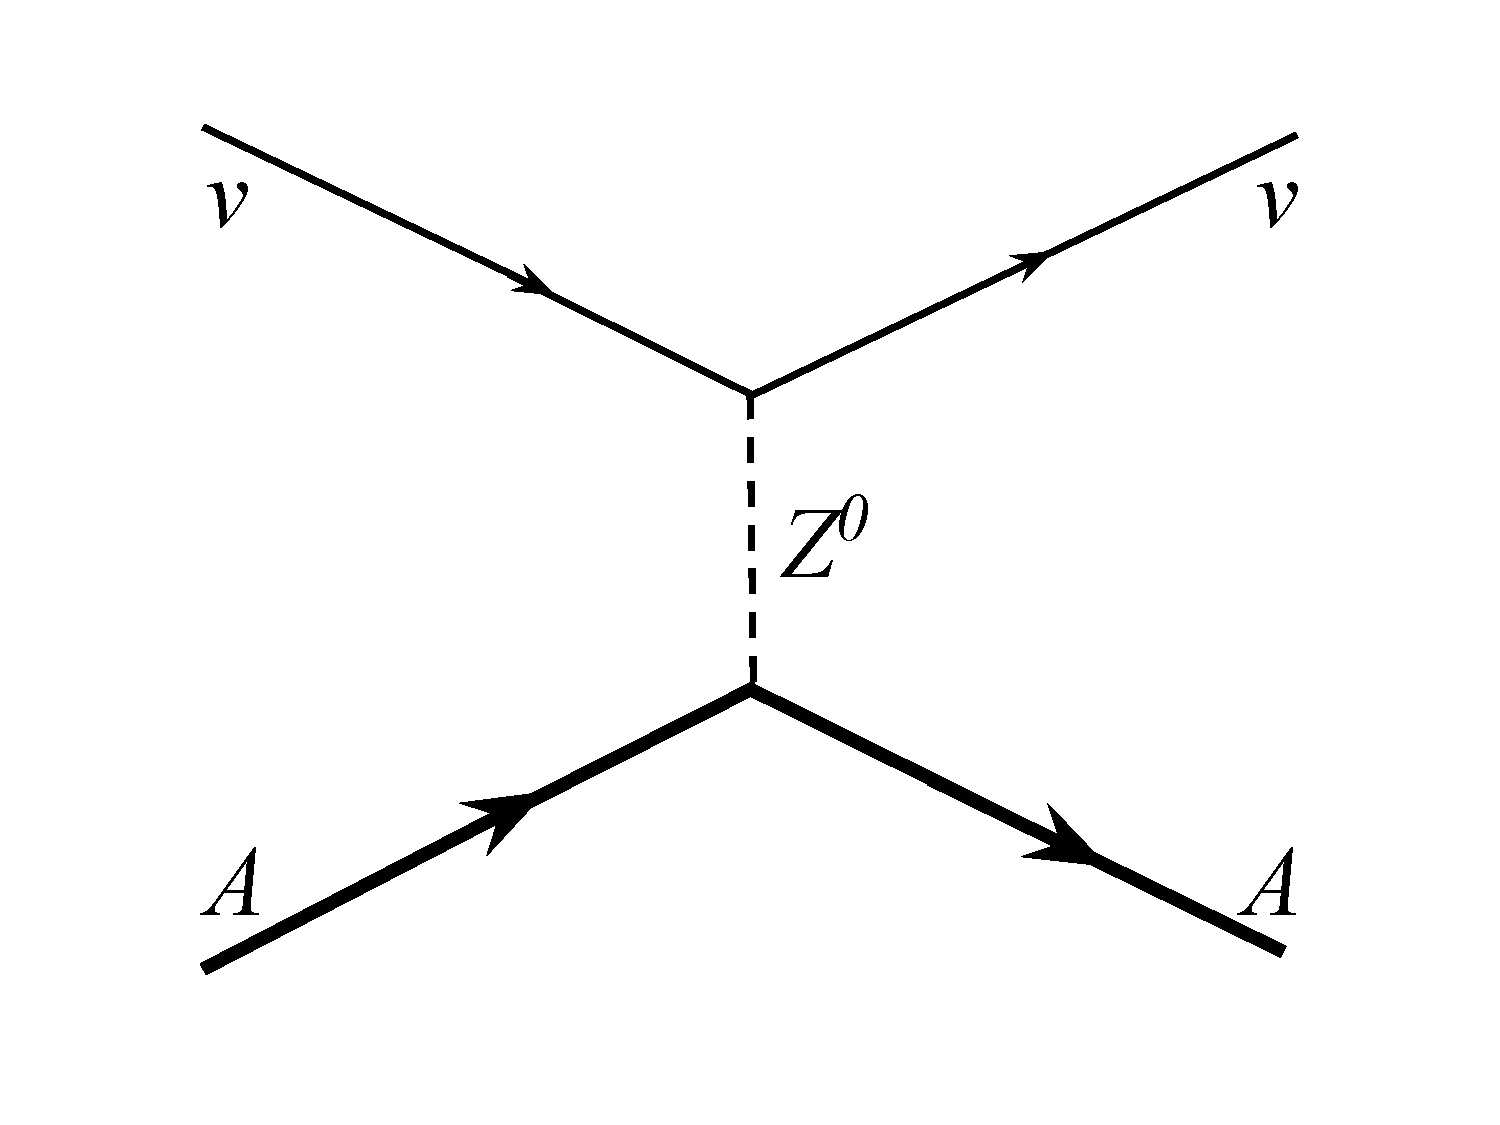
\includegraphics[width=0.6\linewidth]{images/cevns.pdf}}
	\caption{Схема когерентного рассеяния нейтрино на ядре}
	\label{ris:cevns}
\end{figure}
\par Дифференциальное сечение процесса представляется формулой \cite{cevns1, Lindner2017}:
	
\begin{equation}
\frac{d\sigma}{dE_r} = \frac{G_f^2}{4\pi} Q_w^2M\left(1-\frac{ME_r}{2E_\nu}\right)F^2(Q^2),
\end{equation}\\
	
	где $G_f$ --- константа Ферми;
	$Q_w=N-(1-4\sin^{2}\theta_w)Z$ --- слабый заряд для ядра с числом нуклонов $N$ и зарядом ядра $Z$;
	$F(Q^2)$ --- форм-фактор;
	$\theta_w$ --- угол смешивания слабого взаимодействия (угол Вайнберга).
	Используя значение угла можно показать, что сечение взаимодействия
	 $\sim N^2$:\\
	 
	$\sin^2(Q_w)\approx 0.22$ $\to Q_w\sim N \to \sigma \sim N^2$\\
	
	Полное сечение процесса приближённо равно:\\
	
	$\sigma \approx 0.4\cdot10^{-44}  N^2$(E$_\nu^2)$см$^{2}$/МэВ. \\
	\par
	Процесс УКРН имеет место при энергии нейтрино менее 50 МэВ, когда длина волны де Бройля для нейтрино не превосходит размеры ядра, и взаимодействие идет когерентно.
	Отметим, максимальная энергия ядра отдачи равна
\begin{equation}
    T_{max} = \frac{2E_{\nu}^{2}}{M+2E_{\nu}},
    \label{Tmax}
\end{equation}
то есть для большинства элементов энергия ядра отдачи очень мала --- порядка единиц-десятков кэВ на ядро. Таким образом возникают серьезные экспериментальные трудности при регистрации подобных процессов.
\subsection{Эксперименты по исследованию УКРН}
\label{subsect1_1_2}
Долгое время, несмотря на наличие теоретического предсказания, эксперименты по исследованию упругого когерентного рассеяния нейтрино не проводились. Это связано с экстремально низкой, как следует из формулы \ref{Tmax} (единицы-десятки кэВ) энергией ядра отдачи, что предъявляет серьезные требования к экспериментам, уровням шумов электроники и внешних фонов. В последние годы прогресс в области низкофоновых экспериментов сильно шагнул вперед во многом благодаря возросшему интересу к темной материи. 
\par Впервые процесс УКРН был зарегистрирован коллаборацией COHERENT в 2017 году на детекторе CsI[Na]~\cite{COHERENT:2017ipa}. Эксперимент коллаборации COHERENT был поставлен на ускорителе SNS в Окриджской Национальной Лаборатории в США. %Молекулы Cs и I имеют очень близкие атомные номера (78 и 74), что приводит к тому, что эффективный атомный номер позволяет сделать достоверные выводы о зависимости сечения от характер данного процесса от атомного номера по полученным данным. 
Через несколько лет успех коллаборации был повторен и УКРН было зарегистрировано на ядрах аргона \cite{PhysRevLett.126.012002}, что позволяет сделать достоверные выводы о зависимости сечения от характер данного процесса от атомного номера по полученным данным. На данный момент в мире существует более 10 экспериментов по исследованию УКРН. Среди них есть эксперименты как на ускорителях \cite{COHERENT:2018gft}, так и на реакторах \cite{Belov_2015, Aguilar-Arevalo_2016, ricochet, Buck_2020, Singh:2016glu, Strauss_2020, Chaudhuri:2022pqk}. 

\section{Двухфазный метод регистрации частиц} 
\label{sect1_2} 
\subsection{История создания и основной принцип работы}
\label{sect1_2_1}
Детекторы на сжиженных благородных газах разной сложности использовались в экспериментальной физике для регистрации частиц много лет \cite{Chepel_2013}. Благородные газы, такие как аргон и ксенон отличаются рядом преимуществ, которые позволяют масштабировать детекторы до большого (вплоть до нескольких тонн рабочего вещества) объема, регистрировать события малой (единицы-десятки кэВ) энергии. Кроме того, они легко поддаются очистке за счет своей инертности.  В 1970 году Б.А. Долгошеиным был предложен~\cite{Dolgoshein} метод, основанный на использовании двух фаз рабочего вещества. Схема работы метода изображена на рисунке \ref{img:twophase}.

\begin{figure}[h]
	\center{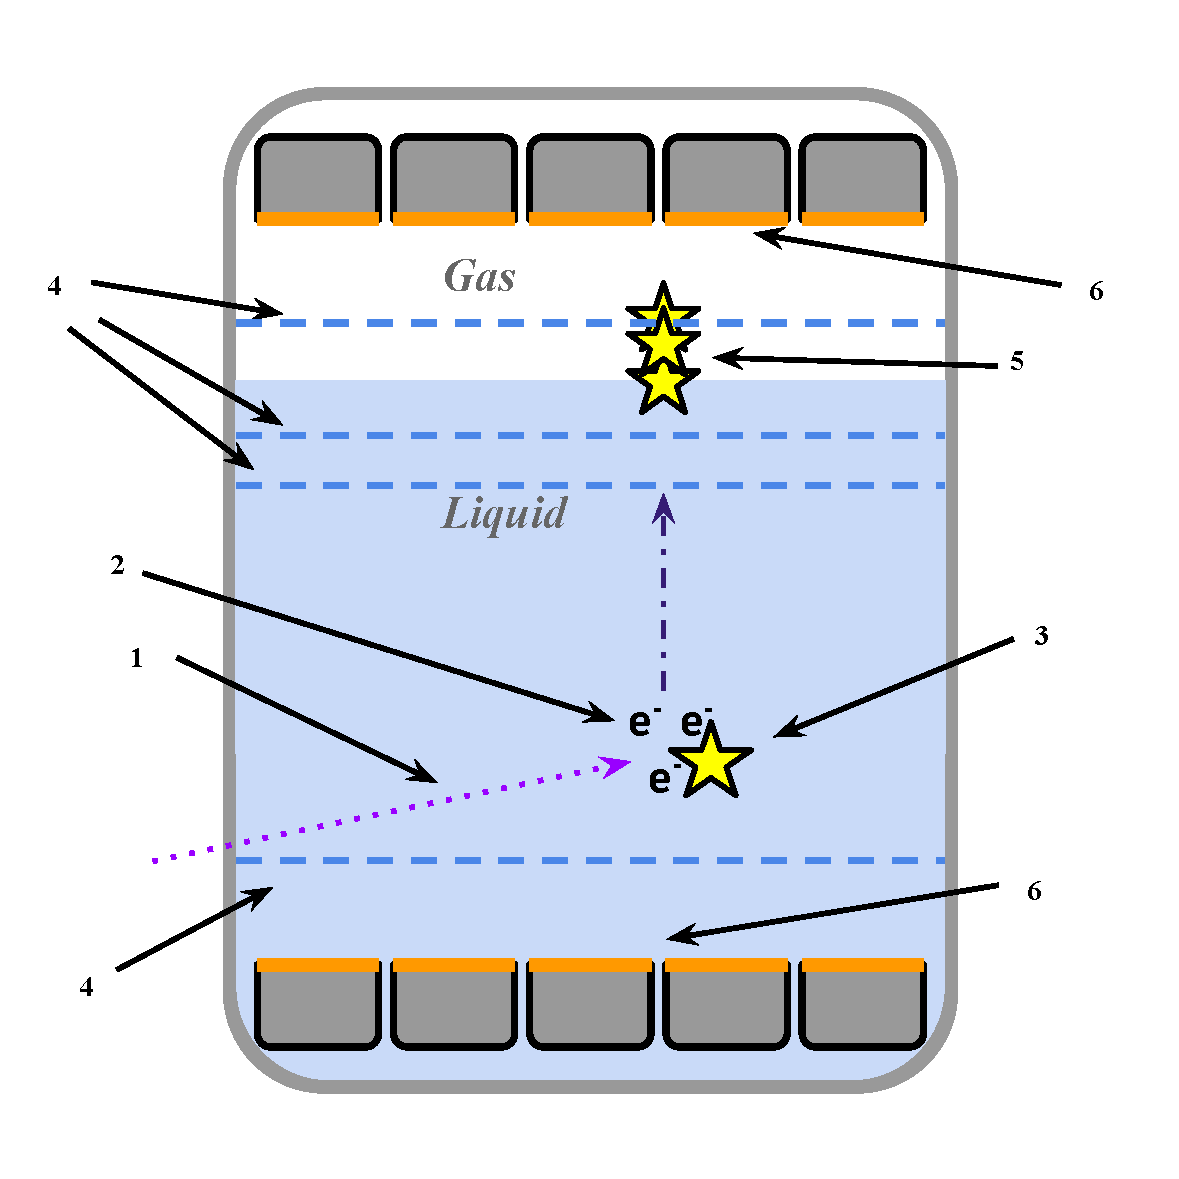
\includegraphics[width=0.7\linewidth]{images/twophasedetector.pdf}}
	\caption[Схема работы двухфазного детектора.] {1 -- трек ионизирующей частицы; 2 -- электроны ионизации, возникшие в результате взаимодействия; 3 -- вспышка сцинтилляции (S1), возникшая в результате взаимодействия; 4 -- электроды-сетки, создающие напряжение; 5 -- электролюминесценция (S2) в электролюминесцентном зазоре; 6 -- матрицы из фотоумножителей}
	\label{img:twophase}
\end{figure}

При взаимодействии элементарной частицы с ксеноном испускаются фотоны сцинтилляции (S1) и электроны ионизации.  Электроны ионизации под действием приложенного электрического поля дрейфуют к границе раздела фаз. После выхода в газовую газе электроны возбуждают атомы ксенона с излучением вторичной сцинтилляции (S2), также называемой электролюминесценцией. Следует подчеркнуть, что размножение электронов отсутствует, следовательно количество фотонов пропорционально количеству электронов. Регистрация сцинтилляции и электролюминесценции происходит за счет фотоумножителей, расположенных сверху и снизу от рабочего объема. Временной промежуток между S1 и S2 вкупе с информацией о скорости дрейфа электронов позволяют рассчитать глубину произошедшего события, а распределение света по матрицам фотоумножителей — координаты в горизонтальной плоскости и полную энергию события. Трехмерная реконструкция событий позволяет создавать так называемые детекторы  "без стенок"\, выделяя внутри детектора отдельный рабочий объем (FV - fiducial volume), содержащий малое количество событий из внешнего фона, что особенно важно если речь идет о поиске редких событий с низкой энергией.

\subsection{Двухфазные детекторы в современной экспериментальной физике}
\label{sect1_2_2}
Двухфазные детекторы нашли широкое применение в низкофоновой физике. В основном это эксперименты по исследованию темной материи~\cite{BOLOZDYNYA2015405}. Первым двухфазным детектором "без стенок" был XENON10, содержащий 5 кг жидкого ксенона в FV. Этот детектор послежил прототипом проектов XENON100~\cite{Xenon10} и XENON1T~\cite{Xenon100}, содержащих 100 и 1100 кг жидкого ксенона в FV, соответственно. Также ксенон в качестве рабочего вещества используется в детекторах экспериментов LUX, Zeplin, LZ~\cite{LZ} и Panda-X~\cite{Xiao:2017vys}. Жидкий аргон используется в экспериментах DarkSide~\cite{DarkSide:2014llq}, DUNE~\cite{Chardonnet_2020}.
\par Отличительной чертой всех экспериментов по исследованию темной материи явлется расположение глубоко под землей. Толща породы обеспечивала естественное экранирование от космических лучей. Детектор РЭД-100 раполагался на поверхности Земли, что потребовало модификации двухфазного метода регистрации с учетом повышенного фона от космических мюонов.            % Глава 1
\chapter{Эксперимент РЭД-100} 
\label{chapt2}
В 2021-22 гг. на реакторе четвертого энергоблока Калининской АЭС был поставлен эксперимент РЭД-100 по исследованию УКРН ~\cite{The_RED100_Experiment}. Это один из немногих экспериментов, поставленных на промышленном реакторе. РЭД-100 был создан прицельно для измерения УКРН. Постановке эксперимента на Калининской АЭС предшествовал длительный подготовительный процесс в ЛЭЯФ НИЯУ МИФИ, включавший в себя наладку оборудования и инженерные запуски. 
\section{Детектор РЭД-100}
\label{sect2_1}
\subsection{Устройство детектора РЭД-100}
\label{subsect2_1_1}
Детектор РЭД-100 представляет собой двухфазный эмиссионный детектор. Рабочим веществом данного детектора является ксенон, однако данный детектор может быть модифицирован для работы и с другими благородными газами. Схема детектора РЭД-100 приведена на рисунке \ref{img:detscheme}. Общий вес ксенона в системе РЭД-100 составляет около 200 кг, при этом вес непосредственно рабочего объема, участвующего в регистрации частиц -- 130 кг. 
\begin{figure}[H]	\center{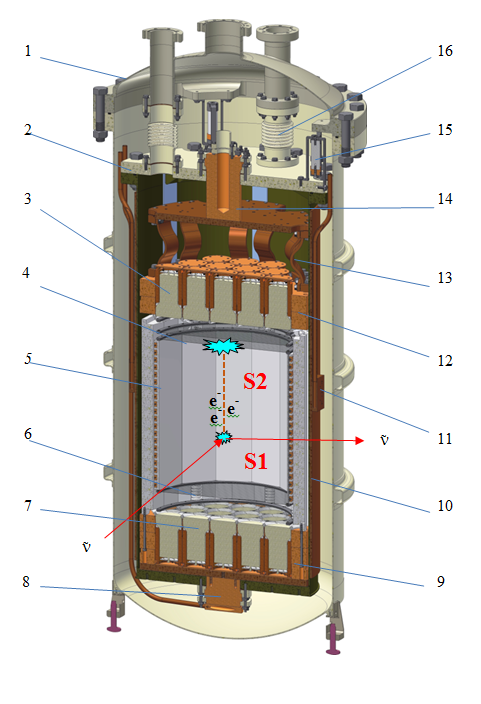
\includegraphics[width=0.5\linewidth]{images/red100.png}}
	\caption[Принцип работы и устройство детектора РЭД-100] {[Принцип работы и устройство детектора РЭД-100. 1 --- внешний сосуд титанового криостата, 2 --- внутренний сосуд титанового криостата, 3 --- верхняя матрица из девятнадцати ФЭУ типа Hamamatsu R11410-20, 4 --- сетчатый анод и электронный затвор, 5 --- рабочий объем, окруженный тефлоновым отражателем со встроенными полезадающими электродами, 6 --- сетчатый катод, 7 --- нижняя матрица из девятнадцати ФЭУ, 8 --- нижний центральный теплосъемник с термосифоном, 9 --- медная обойма для нижней матрицы ФЭУ, 10 --- медный кожух холодного сосуда криостата, 11 --- один из двух боковых теплосъемников с термосифонами, 12 --- медная обойма верхней матрицы ФЭУ, 13 --- гибкий тепловой мост, 14 --- верхний центральный теплосъемник с медным диском, на котором конденсируется ксенон, 15 --- теплоизолирующий подвес, 16 --- сильфонная тепловая развязка для вывода кабелей; $e^-$ --- электроны ионизации, $\overline{\nu}$ --- антинейтрино, передающее энергию ядру отдачи, S1 --- сцинтилляционная вспышка, S2 --- электролюминесцентная вспышка.}
	\label{img:detscheme}
\end{figure}

\par Внутренний объем криостата (2) содержит электродную структуру, необходимую для создания электрических полей в детекторе. Основная электродная структура состоит из сетчатых электродов катода (6), расположенного снизу, гейта и анода (4) для создания однородного сильного электрического поля в газовой фазе над поверхностью жидкости, а также системы полезадающих колец. Сетчатые электроды представляют из себя плоские травленые сетки из нержавеющей стали с гексагональными ячейками, обладающие коэффициентом оптической прозрачности около 80\%. Они обеспечивают небольшое дрейфовое поле в жидкости; поле, вытягивающее электроны из жидкости в газ, а также сильное поле в газе, в котором происходит электролюминесценция. Система полезадающих колец состоит из 20 кольцевых (12-гранных) эквидистантных электродов, создающих равномерно распределенный электрический потенциал по высоте дрейфового объема. 
\par Рабочий объем детектора заключён внутри электродной системы и просматривается фотоэлектронными умножителями (ФЭУ) Hamamatsu R11410-20, размещенными в виде двух матриц – верхней (3) и нижней (7), по 19 ФЭУ в каждой. Этот тип ФЭУ специально разработан японской фирмой Hamamatsu для низкофоновых эмиссионных детекторов на жидком ксеноне. Фотоумножители предназначены для работы при криогенных температурах (-100°С) и чувствительны к длине волны 175 нм с эффективностью регистрации квантовой эффективностью порядка 30\%. Каждый из установленных в детекторе ФЭУ прошел предварительную процедуру характеризации при комнатной температуре, включающую измерение одно-фотоэлектронных характеристик, темнового счета, временных спектров следования после-импульсов и ряда других параметров\cite{Akimov2017}. Характеризация ФЭУ показала, что они имеют хорошее одно-фотоэлектронное разрешение и достаточно высокое внутреннее усиление ($\sim 5\cdot10^6$) сигнала при средних величинах напряжения питания $\sim 1500$ В. 
\par Рабочий объем представляет собой 12-гранную призму с боковыми гранями, выполненными из светоотражающих тефлоновых пластин. Пространство между полезадающими кольцами и стенками внутреннего корпуса криостата заполнено тефлоном, играющим роль вытеснителя ксенона. Фотоумножители располагаются в специальных медных обоймах (9) и (12), которые находятся в тепловом контакте с верхним (14) и нижним (8) термосифонными теплосъёмноками. Тепловой контакт с верхним теплосъёмником осуществляется при помощи гибкого теплового моста, изготовленного из многослойной медной фольги (13). Боковая поверхность внутреннего сосуда криостата снаружи покрыта медным кожухом для выравнивания температурных градиентов. На медном кожухе установлены боковые термосифонные теплосъемники (11).
\par
\begin{figure}[ht]
  \begin{minipage}[ht]{0.64\linewidth}    \center{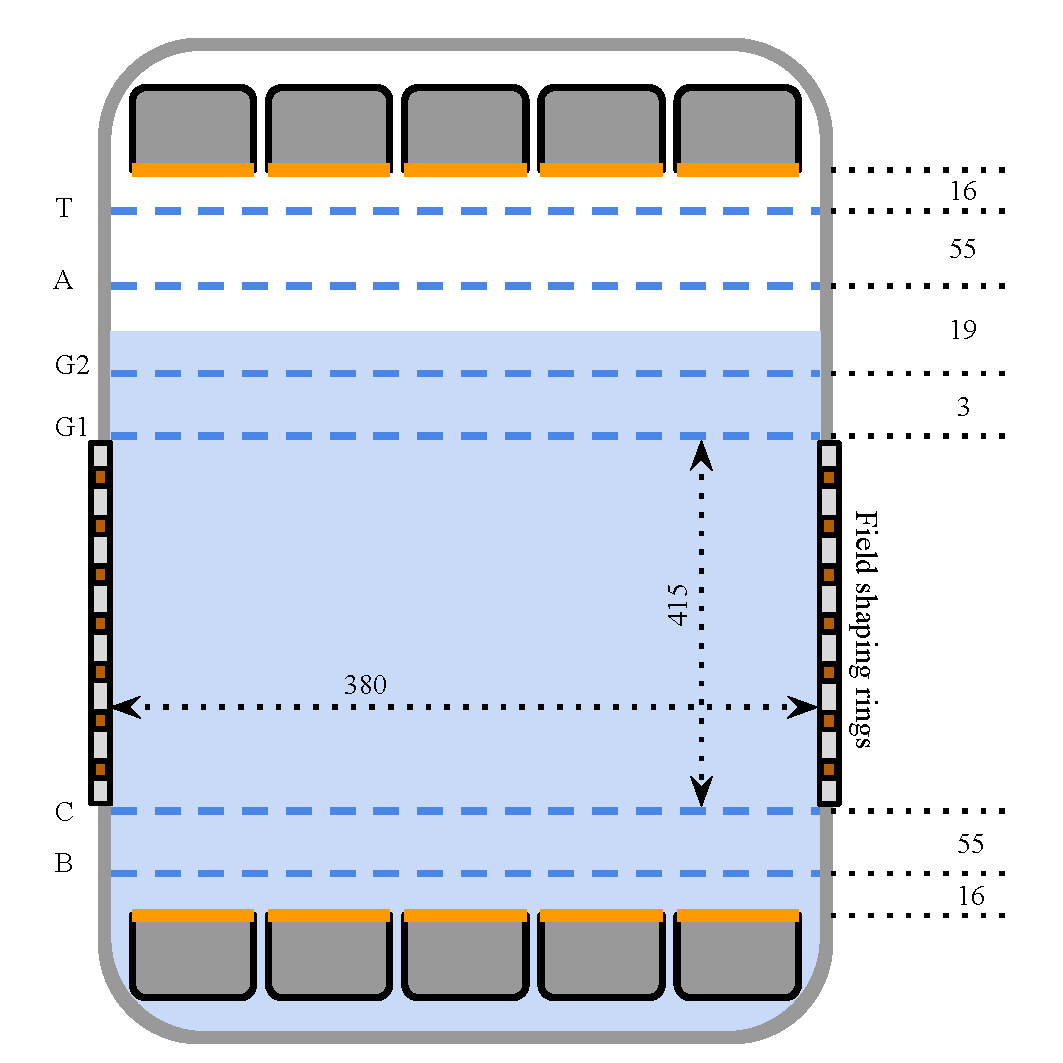
\includegraphics[width=1.0\linewidth]{images/red100grids.pdf} \\ а)}
  \end{minipage}
  \hfill
  \begin{minipage}[ht]{0.34\linewidth}  \center{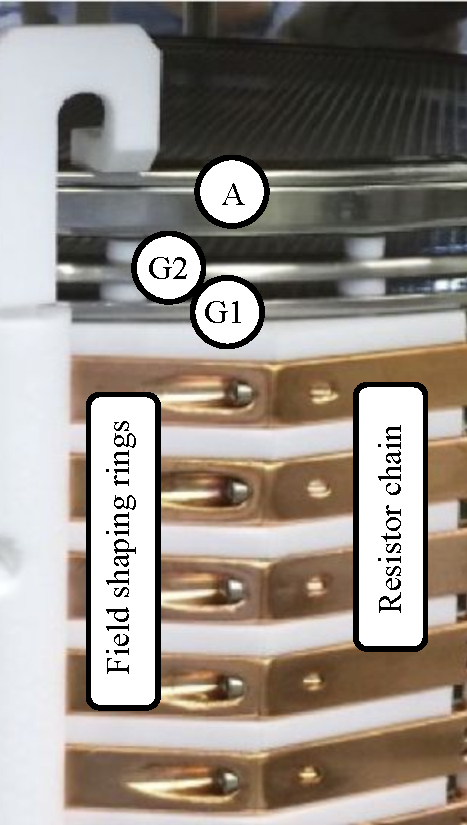
\includegraphics[width=1.0\linewidth]{images/red100electrodes.pdf} \\ б)}
  \end{minipage}
  \caption[Схема и фото электродной системы детектора РЭД-100] {Схема (а) и фото (б) электродной системы детектора РЭД-100. А – сетчатый анод; С – сетчатый катод; В и Т – экранирующие сетчатые электроды под земляным потенциалом; G1 и G2 – сетчатые электроды электронного затвора; Field shaping rings – медные полезадающие электроды;  Resistor chain – цепочка резисторов между полезадающими электродами для создания между ними разности потенциалов. Все размеры приведены в мм.}
  \label{img:red100electrodes}  
\end{figure}

\begin{figure}[ht]	\center{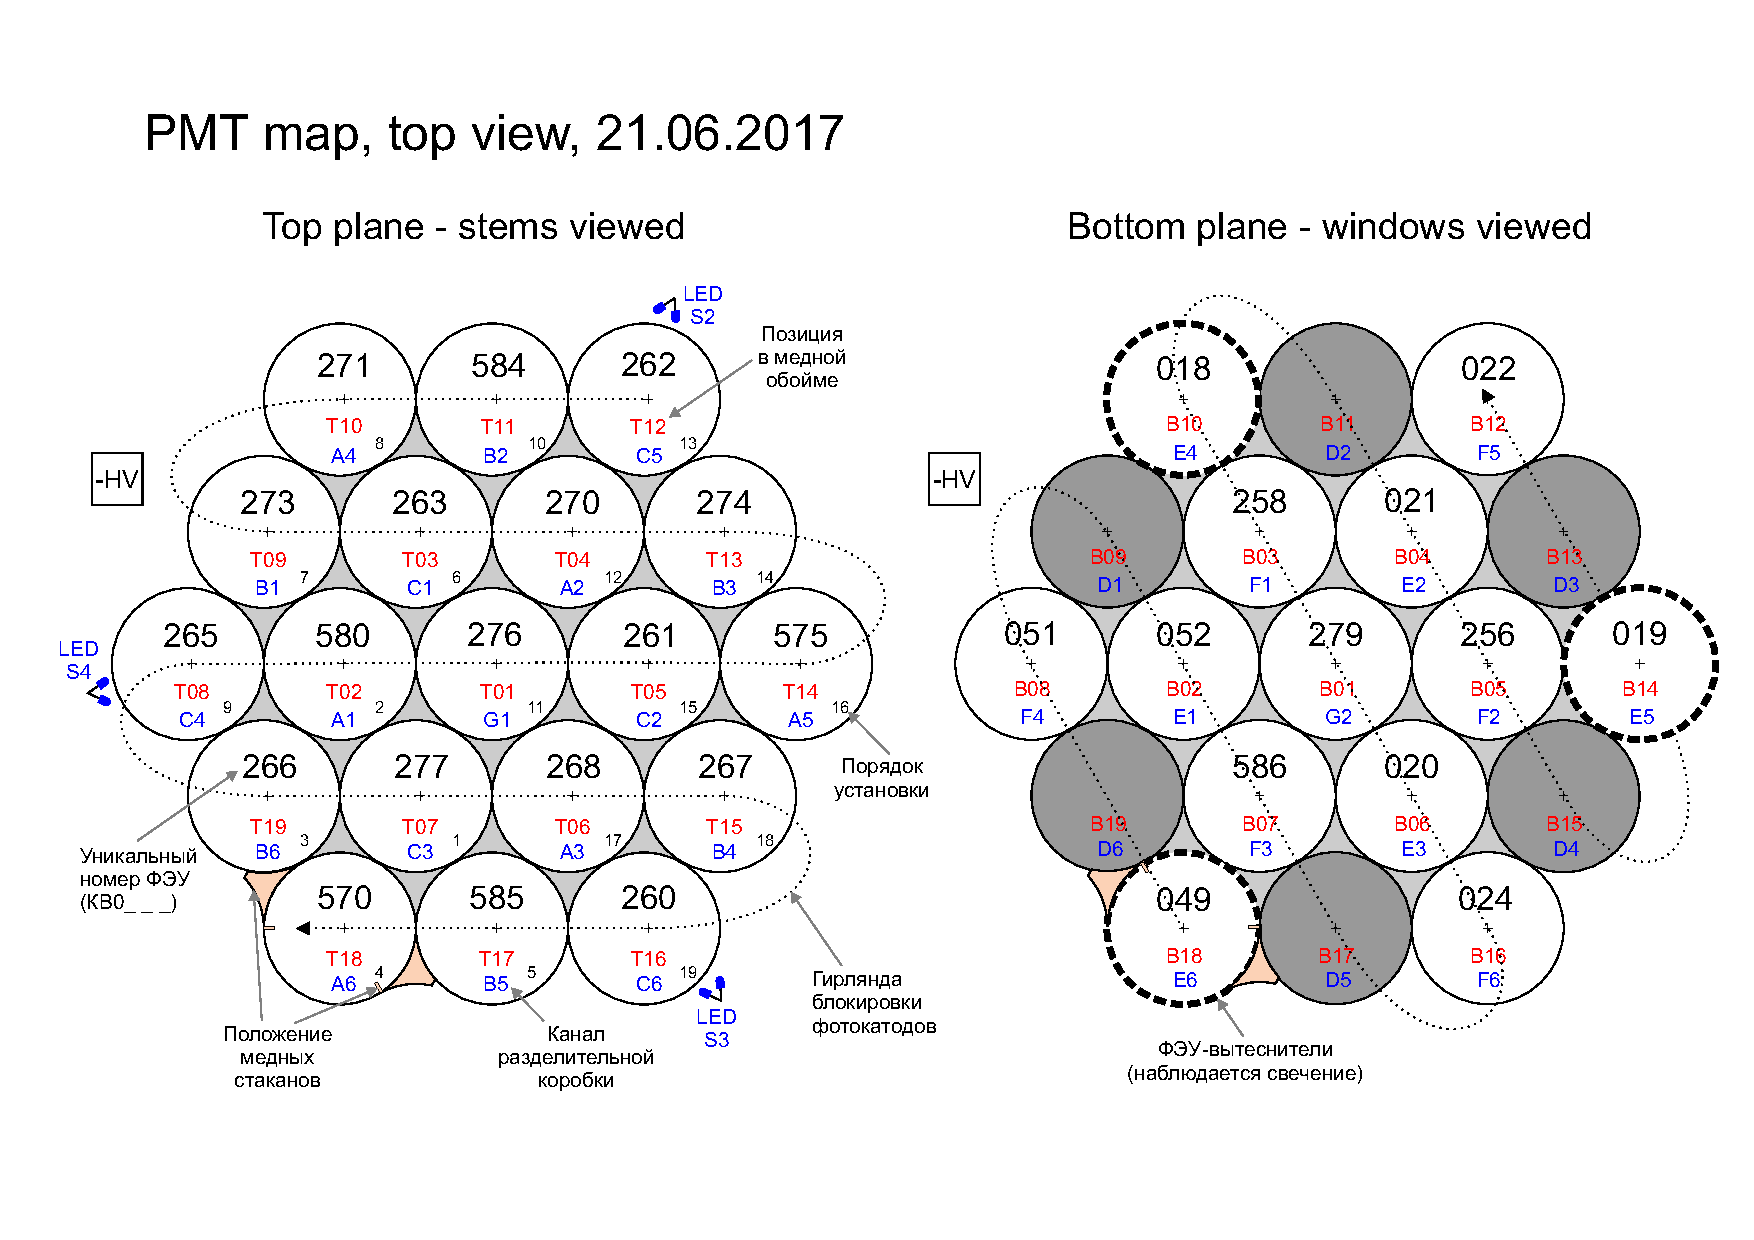
\includegraphics[width=0.9\linewidth]{images/PMT_map_21.06.2017 (1).pdf}}
	\caption[Расположение фотоумножителей в матрице считывания.] {Cлева – в верхней, справа – в нижней; в обоих случаях показан вид сверху; значком -HV показана ориентация матриц относительно катодного высоковольтного кабеля; LED – положения светодиодов вблизи верхней матрицы}
	\label{img:pmtscheme}
\end{figure}

\par Детальное устройство детектирующей части, состоящей из электродной структуры и двух матриц фотоэлектронных умножителей, показано на рисунке \ref{img:red100electrodes} (а). Схема расположения ФЭУ показана на рисунке \ref{img:pmtscheme}. Электродная система включает T - экранирующий электрод верхней матрицы фотоумножителей, находящийся постоянно под земляным потенциалом; А – анод, на который подается положительный потенциал порядка +5 кВ; G2 – подповерхностный электрод, обеспечивающий сильное электрическое поле в газовой фазе детектора, на который подается потенциал порядка -5 кВ; G1 – электрод, обеспечивающий блокировку прохождения электронов к поверхности в случае, когда в детекторе произошло событие с очень большим энерговыделением (описание работы затвора см. ниже), потенциал на нем в режиме пропускания электронов поддерживается равным потенциалу электрода G1, в режиме блокировки потенциал смещается на +300 В; С – катод, потенциал которого -12 кВ; B – экранирующий электрод нижней матрицы, находящийся постоянно под земляным потенциалом. Для создания равномерного электрического поля в дрейфовой области в тефлоне между электродами G1 и C размещены круговые полезадающие электроды. Потенциал на этих электродах задается равномерным делителем собранным между электродами G1 и C при помощи резисторов с сопротивлением 1 ГОм (рисунок \ref{img:red100electrodes} (б)). Полное сопротивление делителя 18 ГОм.
\par Все сетки в детекторе электрополированные и изготовлены из фольги из нержавеющей стали толщиной 0.2 мм с электролитически сформированными гексагональными открытыми ячейками (оптический коэффициент прозрачности ~0.8). Внутренний размер шестиугольного отверстия ячейки - 3.5 мм, ширина перемычки между соседними ячейками 0.2 мм. Сетки в натянутом состоянии приварены точечной контактной сваркой к кольцам из нержавеющей стали.
\parТакже в РЭД-100 были реализованы технологии электронного затвора и блокировки ФЭУ с целью недопущения непреднамеренной регистрации больших сигналов от космических мюонов. 

	
Событие, соответствующее прохождению космического мюона через детектор, представляет собой практически непрерывное свечение, образованное выходом большого количества электронов с трека мюона в газовую фазу. Поскольку мюон  в среднем теряет в объеме детектора около 200 МэВ, сигнал электролюминесценции оказывается слишком большим для нормальной работы фотоумножителей, что при длительном воздействии такой сильной засветки на фотокатоды приводит к их деградации. Для предотвращения “выгорания” фотокатодов фотоумножителей производится выключение эмиссии фотоэлектронов с фотокатодов путем подачи на 1-ые диноды (одновременно всех фотоумножителей) положительного смещения величиной около 300 В (равной характерной разности потенциалов между фотокатодом и первым динодом). Этот сигнал вырабатывается триггерным модулем по приходу сцинтилляционного сигнала, превышающего соответствующий амплитудный порог. Данный сигнал также подается на электронный затвор (на электрод G2) для предотвращения прохождения электронов от мюона в область электролюминесценции. Предотвращение прохождения электронов к поверхности жидкого ксенона при большом энерговыделении в рабочем объеме позволяет снизить шум одиночных электронов за счет минимизации компоненты, вызванной спонтанным выходом с поверхности электронов, находящихся там в потенциальной яме. Более подробно данные технологии, а также устройство детектора РЭД-100 описано в диссертации А. В. Хромова \cite{Khromov_thesis}.

\subsection{Система циркуляции и очистки}
\label{subsect2_1_2}
%+более общие слова, что мы меряем ионизационный сигнал и нам не нужно его терять
\parОсновным источником измеряемого сигнала в детекторе РЭД-100 является электролюминесценция, производимая электронами ионизации. При дрейфе электронов к границе раздела фаз происходят потери, связанные с захватом дрейфующих электронов электроотрицательными примесями. Для минимизации этих потерь требуется тщательная подготовка рабочего вещества. В процессе хранения и транспортировки чистота рабочего вещества деградирует и требуется дополнительная циркуляция через очищающие геттеры, так как детекторы, подобные РЭД-100 требуют особо высокой чистоты рабочего вещества. Для измерения чистоты ксенона мы опираемся на производное выражение в виде среднего времени жизни свободных электронов в жидком ксеноне. 
%спросить у акимова, что со связью концентрации и времени жизни
%TODO подумать про то как модифицировать текст этого абзаца
\parСистема газообеспечения (система хранения и очистки газа и система вакуумной откачки) установки РЭД-100 включает в себя стандартные газовые элементы, такие как баллоны высокого давления для хранения ксенона, безмасляные вакуумные насосы, элементы газовых коммуникаций, циркуляционный насос, манометры и вакуумметры с металлическими уплотнениями, электронные элементы контроля давления газа и вакуума, горячий металлический геттер SAES MonoTorr. Система позволяет осуществлять циркуляционную очистку ксенона по замкнутому контуру и поддерживать необходимый уровень чистоты ксенона. Газовая система детектора РЭД-100 является системой закрытого типа, то есть не имеющей контакта с атмосферой. При неработающем детекторе РЭД-100 ксенон хранится в алюминиевых баллонах Luxfer под давлением 50 атмосфер. 
\parДетектор соединён с газовой системой через интерфейсный блок при помощи трех сильфонных металлорукавов внутренним диаметром 68 мм и длиной 4 м. Один из этих металлорукавов содержит высоковольтные кабеля, другой - сигнальные кабеля, третий - сильфонный теплообменник для минимизации теплопритока при циркуляции ксенона через систему очистки ксенона. При работе детектора металлорукава продуваются постоянным потоком газообразного ксенона, поступающего из системы очистки с потоком порядка 1 л/мин. На входе в газовую систему каждый канал циркуляции оборудован контрольным расходомером MKS1479D.  Поток газа в каждой линии устанавливается и регулируется программным образом. После прохождения газообразного ксенона через геттер газообразный ксенон возвращается в детектор по замкнутому контуру, конденсируется и в жидком виде поступает в детектор. 

\subsection{Система термостабилизации}
\parДля охлаждения детектора RED-100 и поддержания его при температуре жидкого ксенона используется криогенная система, основанная на термосифонной технологии (гравитационная тепловая труба)~\cite{red100cryo}. Эта технология имеет ряд преимуществ по сравнению с другими известными системами охлаждения и термостабилизации: уменьшенное количество радиоактивных элементов вблизи активного объема детектора, значительно более низкий уровень механических колебаний, низкий расход хладагента и способность работать без электроэнергии. Термосифон криогенной системы RED-100 представляет собой вертикально ориентированную закрытую трубку, которая может быть функционально разделена на следующие три части: сверху - конденсатор, погруженный в сосуд Дьюара со свободно кипящим жидким азотом; внизу испаритель (охлаждающая головка), термически контактирующий с детектором, и пассивная адиабатическая часть между этими двумя частями. Трубка заполнена газообразным азотом. Эффективный отвод тепла от детектора достигается фазовым переходом азота внутри термосифона. Газ конденсируется в конденсаторе и стекает в испаритель. Там он закипает от тепла, отводимого от детектора, и поднимается вверх к конденсатору, и таким образом, процесс непрерывно циклически повторяется. Теплопроводность термосифонов может достигать очень высоких значений, порядка нескольких десятков кВт/К·м, что сопоставимо с теплопроводностью углеродных нанотрубок. Термостабилизация детектора RED-100 осуществляется путем изменения тепловой проводимости термосифона (охлаждающей способности), что, в свою очередь, осуществляется путем изменения количества газообразного азота внутри трубки, соединяющим теплосъёмник, установленным в месте поглощения тепловой энергии, с конденсором, установленным внутри термосифонного сосуда Дьюара, в котором происходит ожижение азота. В детекторе RED-100 имеются четыре термосифона с общей мощностью охлаждения до $\sim$ 400 Вт.
\parТермосифонная криогенная система обеспечивает конденсацию около 200 кг жидкого ксенона в течение порядка суток (до 10 л/мин газа при н.у., или 60 г/мин) и позволяет поддерживать жидкий ксенон внутри детектора RED-100 при постоянной температуре в диапазоне от 165 до 175 К с точностью <0,2 К, а также обеспечивать вертикальный градиент температуры <1 К/м, чтобы минимизировать конвекционные потоки жидкого ксенона внутри чувствительного объема, которые могут повлиять на характеристики детектора.

\subsection{Система сбора данных}
\label{subsect2_1_3}
Сбор данных осуществляется с помощью специализированной системы и заключается в приеме сигналов из детектора, усилении/формировании этих сигналов, генерации триггера и сохранении оцифрованных данных на диск. Эти действия производятся модулями электроники и компьютером data acquisition (DAQ). Система является централизованной. 
\par В рамках эксперимента РЭД-100 требуются надежные идентификация и измерение одиночных фотоэлектронов ФЭУ в рамках окна записи больше максимального времени дрейфа в электролюминесцентном зазоре, поэтому производится запись полных форм сигналов. 
\parПосле регистрации фотонов ФЭУ формируют электрические сигналы, выведенные из детектора через интерфейсный модуль. Сигналы усиливаются быстрыми малошумящими усилителями Phillips Scientific 777. Усилители имеют полосу пропускания от 0 до 200 МГц и регулируемый коэффициент усиления в диапазоне 2x–50x, что обеспечивает дополнительную свободу для выравнивания усиления ФЭУ. Сигнал с усилителей отправляется непосредственно на АЦП, а также на линейный разветвитель Phillips Scientific 748 для формирования триггера. Для записи форм сигналов используются модули аналого-цифрового преобразования (АЦП) прямого преобразования CAEN V1730. Модули обеспечивают оцифровку форм сигналов с частотой 500 млн. отсчетов/с и разрешением 14 бит, память модуля позволяет хранить 5 млн. отсчетов для каждого канала. В режиме максимальной чувствительности модуль обеспечивает шаг бинирования 0.03 мВ и 2 нс, что вполне достаточно для надежной регистрации одиночных фотоэлектронов. В основном режиме работы детектора ФЭУ работают в режиме, обеспечивающем амплитуду одно-фотоэлектронных импульсов $\sim$ 1 мВ.

\textbf{Триггер}
\parБольшие различия основных режимов работы накладывают повышенные требования на схему формирования триггера, как в части нижнего порога, так в отношении динамического диапазона. Для решения всех возложенных задач триггерная схема реализована на базе цифрового модуля программируемой логики CAEN V1495. Общая схема триггера приведена на рисунке \ref{img:trigger}. Режим наибольшей чувствительности оптимизирован на отбор событий с сигналами от 1 до 10 электронов ионизации. Его работа построена на пересчёте количества срабатываний поканальных дискриминаторов (CAEN V895), настроенных на порог $\sim$1/3 от амплитуды однофотонных импульсов, в бегущем окне длиной 2 мкс, что соответствует длине электролюминесцентного сигнала. Подсчет ведется независимо по верхним и нижним плоскостям ФЭУ, срабатывание происходит если количество импульсов укладывается в выбранный диапазон, что позволяет отбрасывать случайные совпадения и большие сигналы.
\begin{figure}[H]
	\center{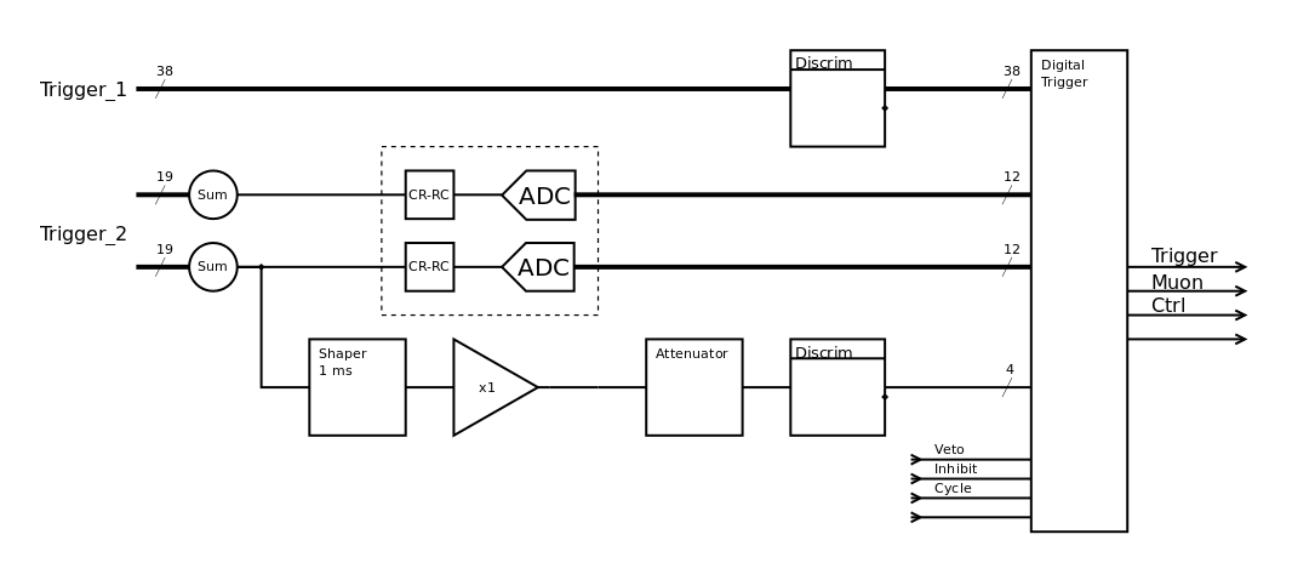
\includegraphics[width=1.0\linewidth]{images/trigger.png}}
	\caption{Блок-схема триггера}
	\label{img:trigger}
\end{figure}
\parДля отбора гамма-квантов производится суммарный сигнал по верхней и нижней плоскостям ФЭУ, получаемый с помощью линейных сумматоров CAEN N625. Эти сигналы отправляются на дополнительные АЦП, которые отправляют результат непосредственно в триггерный модуль. В модуле производится цифровая обработка формы сигналов, что позволяет отбирать события с совпадениями сцинтилляционных и электролюминесцентных сигналов в пределах времени полного дрейфа. Отбор мюонов осуществляется по совпадению сигналов с дискриминаторов с большим порогом (~1В) в нескольких ФЭУ. Триггерный модуль формирует сигналы на блокировку ФЭУ и затвора. Дополнительно триггерный модуль используется для мониторинга состояния детектора путём определения частоты различных событий.


\subsection{Методы калибровки детектора РЭД-100}
\label{subsect2_1_4}
РЭД-100 является крайне сложным и чувствительным прибором. Для детального понимания процессов внутри детектора требуется измерение следующих значений:
\begin{itemize}
    \item площади однофотоэлектронных импульсов SPE (single photo electron) для каждого канала
    \item параметры сигнала (светосбор, длительность) от одного электрона ионизации
    \item параметры эффективности светосбора в детекторе
    \item время жизни электронов при дрейфе в жидкой фазе
    \item ионизационный выход (количество электронов ионизации на единицу энерговыделения в рабочей среде детектора)
    \item коэффициент экстракции электронов при переходе границы раздела фаз
\end{itemize}
\par Для определения указанных параметров необходима комплексная калибровка систем детектора. 
	\parК калибровочным данным можно отнести light emitting diod (LED) калибровку, данные с одноэлектронными (SE -- single electron) сигналами, мюонные данные и гамма калибровочные данные. С некоторыми отличиями, приведенные калибровочные типы данных набирались как при инженерных запусках детектора, так и при постановке эксперимента на Калининской АЭС.
 \begin{enumerate}
     \item\textbf{LED калибровка}
    \parПри наборе данного типа данных триггер запускался от генератора одновременно со светодиодом, расположенного как показано на рисунке \ref{img:pmtscheme}. Это позволяло набрать данные с SPE импульсами и определить параметры однофотоэлектронных импульсов для каждого ФЭУ.
	 \item\textbf{SE-данные}
	\par Цель набора данного типа калибровок -- получение информации о одноэлектронных сигналах с нулевым порогом регистрации. Был использован внешний триггер не зависящий от сигнала внутри детектора. Реализация данного триггера была различной при различных запусках детектора и описана в соответствующих разделах (\ref{subsect2_2_1}, \ref{subsect2_2_2}). Также этот метод позволяет измерить частоту сигналов SE-фона.
	 \item\textbf{Мюонные данные}
	\parНабор мюонных данных используется для определения времени жизни электронов при дрейфе в жидком ксеноне и контроля степени очистки, описанной в разделе \ref{subsect2_1_2}. Для набора данных от космических мюонов детектор переводился в специальный режим, характеризующийся отключением электронного затвора, а также пониженным (до 0.1 мВ на SPE) напряжением на ФЭУ. Отбор мюонов осуществляется по совпадению сигналов с дискриминаторов с большим порогом ($\sim$1В) в нескольких ФЭУ. 
	 \item\textbf{Измерения с гамма-источниками}
	\parБыли использованы гамма-источники $^{60}$Co, $^{22}$Na и $^{137}$Cs. Триггер в данном случае запускался от сцинтилляции. Измерения с гамма-источниками необходимы для энергетической калибровки отклика детектора, измерения энергетического разрешения, а также для построения так называемых функций эффективности светосбора (light response functions -- LRF). Более подробно про LRF и процедуры пространственного восстановления см. \ref{sect3_2}
\end{enumerate}

\subsection{Основные источники фона в детекторе}
\label{subsect2_1_5}
Как и любой детектор, РЭД-100 подвержен воздействию различного типа фонов. Источники фона в РЭД-100 можно разделить на две большие группы:
\begin{enumerate}
    \item Внешние источники фона. К внешним источникам фона относится гамма и нейтронный фон различной природы от окружающих материалов. Также фон от космических мюонов, которые дают гигантский ионизационный сигнал. 
    \item Внутренние источники фона. К внутренним источникам фона относятся, во-первых распады радиоактивных элементов в рабочем веществе детектора, а во-вторых, так называемый фон спонтанной эмиссии, зарегистрированный также и на других детекторах такого типа~\cite{se_akimov, Santos:2011ju}, включающий в себя несколько компонент. Первая компонента вызвана спонтанным выходом электронов с поверхности жидкости, находящихся там в потенциальной яме. Оставшаяся компонента шума представляет собой электроны, вышедшие с трека с задержкой, либо захваченные и с задержкой высвобожденные электроотрицательными примесями (в настоящее время природа данной компоненты остается до конца не выясненной). Наложение подобных задержанных сигналов от многих последовательно приходящих мюонных сигналов образует перманентный фон. Совпадение двух или больше таких сигналов по времени формирует неточечные события, составляющие существенную часть фона. Более подробно об алгоритмах подавления данных событий см. \ref{sect4_2}.
\end{enumerate}

\subsection{Программный пакет REDOffline}
\label{subsect2_1_6}
Для первичной обработки форм сигналов с различных детекторов в ЛЭЯФ НИЯУ МИФИ был разработан программный пакет REDOffline. Несмотря на скрупулезный подход к сбору электроники детектора, на сырых формах сигнала имеются электрические наводки, не всегда известной природы. В программном пакете REDOffline реализована полиномиальная коррекция наводок. 

Следующим этапом обработки, необходимым для всех данных в виде форм сигналов является поиск нулевой линии. Для данной процедуры создается амплитудная гистограмма для каждого канала, среднее значение на которой принимается за нулевую линию.

Завершающий этап первичной обработки -- распознавание и параметризация импульсов на форме сигналов. В REDOffline поиск импульсов реализован с использованием амплитудного порога, зависящего от стандартного отклонения шумовой дорожки.

\parКак правило, перед любыми процедурами анализа данные детектора РЭД-100 проходили обработку пакетом REDOffline, что существенно ускоряло и упрощало дальнейшую работу с данными.


\section{Конфигурация установки при различных наборах данных}
\label{sect2_2}
\subsection{Инженерный запуск в ЛЭЯФ НИЯУ МИФИ 2019 г.}
\label{subsect2_2_1}
\begin{figure}[H]
	\center{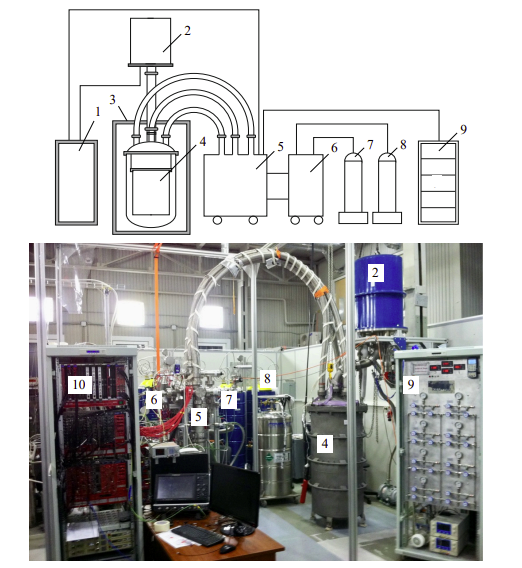
\includegraphics[width=0.8\linewidth]{images/red100_2019setup.png}}
	\caption[Схема установки при инженерном запуске в МИФИ.] {1 -- сосуд Дьюара с жидким азотом, 2 -- криостат термосифонной криогенной системы, 3 -- пассивная защита, 4 -- детектор РЭД-100, 5 -- интерфейсный модуль, 6 -- система очистки ксенона, 7-8 -- хранилище для ксенона, 9 -- система управления термосифонами, 10 -- система сбора данных}
	\label{img:2019scheme}
\end{figure}
В 2019 с помощью детектора был проведен инженерный сеанс установки РЭД-100. Основными целями данного теста являлись проверка различных систем установки, измерения фона и калибровка детектора гамма-источниками. Более подробная информация про данный сеанс и его результаты находится в статье \cite{RED100_2019}. %Конфигурация установки представлена на рисунке \ref{img:2019scheme}. 
\par В рамках данного теста набирались калибровочные данные:
 \begin{enumerate}
     \item LED-калибровка
     \item Мюонные данные
     \item SE-данные. Набор данных производился следующим образом: сохранялись 300 мкс, предшествовавшие срабатыванию триггера на гамма-кванты.
     \item Гамма-калибровки. Для калибровки использовались источники $^{60}$Co и $^{22}$Na. Источник $^{60}$Co был сколлимирован, а при наборе данных с $^{22}$Na была задействована схема совпадений с детектором NaI. 
 \end{enumerate}

\subsection{Эксперимент на Калининской АЭС 2021-22 гг.}
\label{subsect2_2_2}
Калининская АЭС расположена недалеко от города Удомля Тверской области. Состоит из четырех энергоблоков общей мощностью 4000~МВт. 
\begin{figure}[H]
	\center{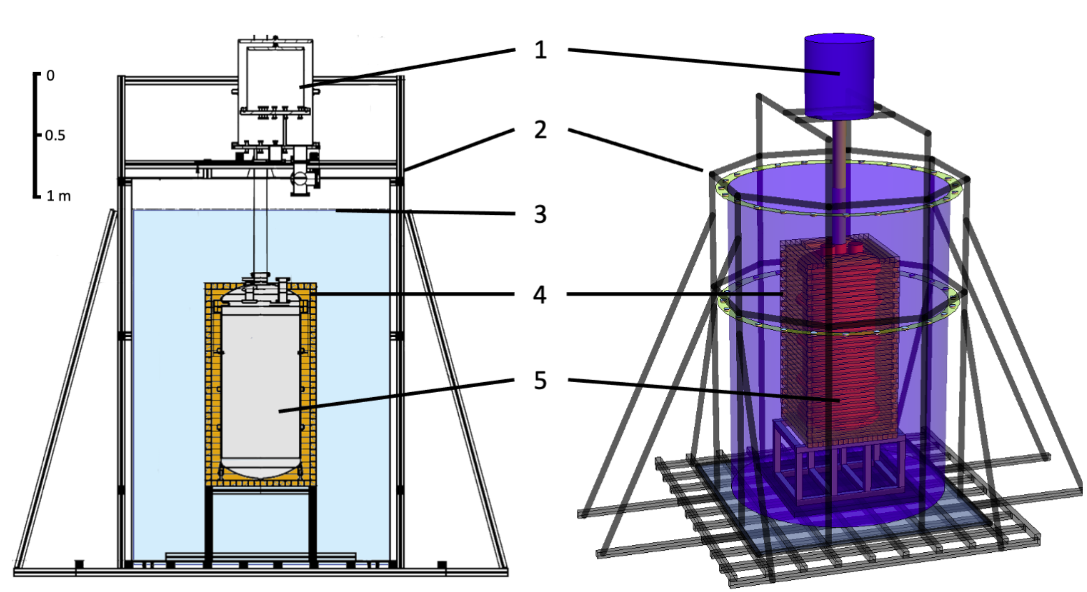
\includegraphics[width=1.0\linewidth]{images/kaes_red100_scheme.jpg}}
	\caption[Схема установки на Калининской АЭС] {Схема установки на Калининской АЭС. 1 -- бак термосифонной системы, 2 -- поддерживающая бак конструкция, 3 -- водный бак, 4 -- медная защита}
	\label{img:kaesscheme}
\end{figure}

\begin{figure}[H]
  \begin{minipage}[ht]{0.49\linewidth}
    \center{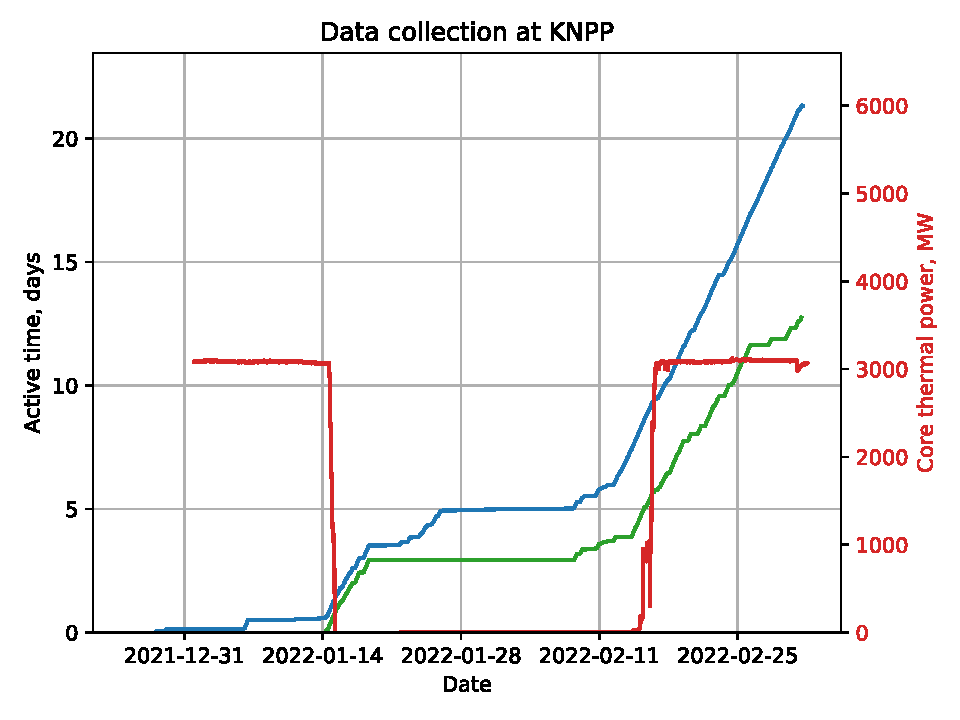
\includegraphics[width=1.0\linewidth]{images/cumulative-time-power.pdf} \\ а)}
  \end{minipage}
  \hfill
  \begin{minipage}[ht]{0.49\linewidth}
    \center{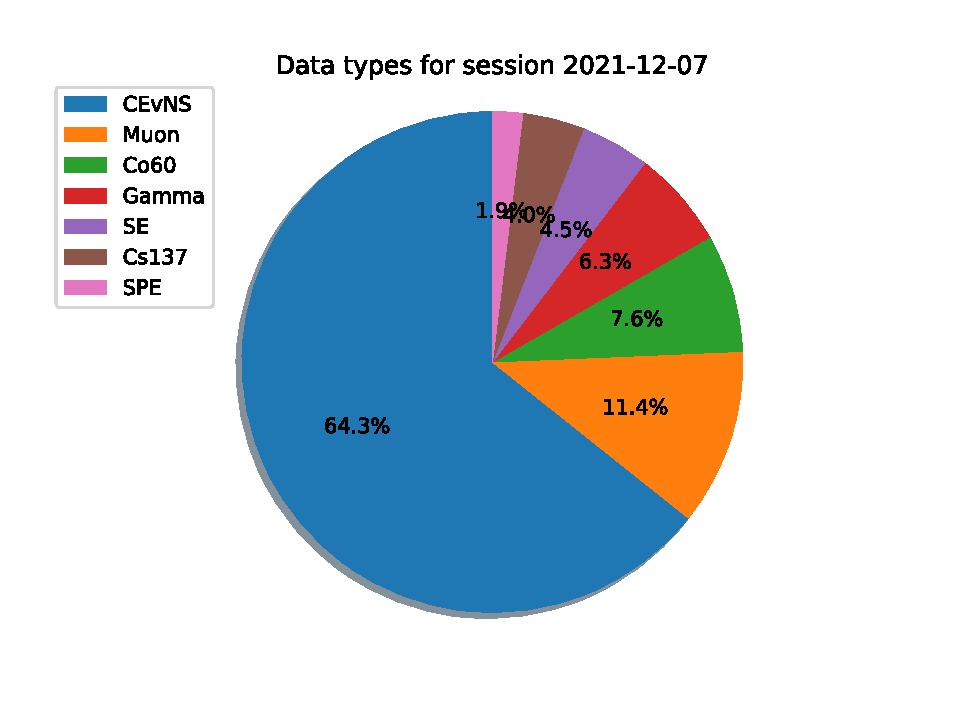
\includegraphics[width=1.0\linewidth]{images/type-pie.pdf} \\ б)}
  \end{minipage}
	\caption[Соотношение набранных типов данных и мощности реактора]{Соотношение набранных типов данных и мощности реактора. Слева -- график мощности реактора (красная линия) и объем набираемых данных различных типов (синяя линия -- все данные, зеленая -- УКРН-подобные данные), справа -- круговая диаграмма показывающая соотношение количества набранных данных различных типов}
	\label{img:datadiagram}
\end{figure}
Детектор РЭД-100 располагался в 19 метрах снизу от реактора 4 энергоблока. В в качестве основной пассивной защиты от космических мюонов выступали бетонные перекрытия здания энергоблока. Далее конструкция детектора была помещена в мягкий бак из ПВХ диаметром 5 м, наполненный водой, что обеспечивало пассивную защиту от нейтронов толщиной 60 см. Для защиты от гамма фона вокруг детектора была выстроена конструкция из медных брусков толщиной 5 см. Схема пассивной защиты детектора РЭД-100 приведена на рисунке \ref{img:kaesscheme}. Более подробная информация о пассивной защите детектора РЭД-100 находится в статье \cite{shielding}.
Мощность реактора в процессе набора данных менялась, ее график приведен на рисунке \ref{img:datadiagram}.  Данные набирались в периоды как с включенным, так и с выключенным реактором для сравнения спектров. 
	Всего набирались шесть основных типов данных:
 \begin{enumerate}
     \item LED-калибровки
     \item Мюонные данные
     \item SE-данные
     \item Гамма-фон
     \item Гамма-калибровки
     \item УКРН-подобные данные
 \end{enumerate}
Соотношение объемов набранных данных различных типов приведено на круговой диаграмме на рисунке \ref{img:datadiagram}.
\parПомимо измерений основным детектором РЭД-100, непрерывно проводились измерения с использованием вспомогательных детекторов, которые были необходимы для понимания фоновых условий эксперимента. К вспомогательным детекторам относятся сцинтилляционные детекторы NaI[Tl] и Bicron, а также два датчика уровня радона Radex.
\parНа протяжении набора данных проводились измерения внешнего гамма-фона, которые показали что фон однороден за исключением нескольких отдельных областей~\cite{The_RED100_Experiment}. Измеренный гамма-фон в помещении на КАЭС приблизительно в 5 раз больше, чем в ЛЭЯФ НИЯУ МИФИ. Это связано с толстыми бетонными стенами, потолком и полом в здании реактора.  На протяжении сеанса набора данных на КАЭС вспомогательный детектор NaI[Tl] был расположен как показано на рисунке \ref{img:kaesscheme}. На рисунке \ref{img:gammaneutronbckg} (а) показан график изменения гамма-фона на протяжении сеанса набора данных. Резкие изменения в начале и в конце набора данных связаны с заполенением бака водной защиты и его осушением, соответственно.
\par Результаты мониторинга нейтронного фона при постановке эксперимента на КАЭС показаны на рисунке \ref{img:gammaneutronbckg} (б). Заметной разницы между нейтронным фоном при включенном и при выключенном реакторе не наблюдалось. 
\par Фон от космических мюонов измерялся непосредственно детектором РЭД-100, так как мюонные данные были необходимы для измерения времени жизни электронов в жидком ксеноне. Мюонный фон также был стабилен во время постановки эксперимента. 

\begin{figure}[H]
  \begin{minipage}[ht]{0.49\linewidth}
    \center{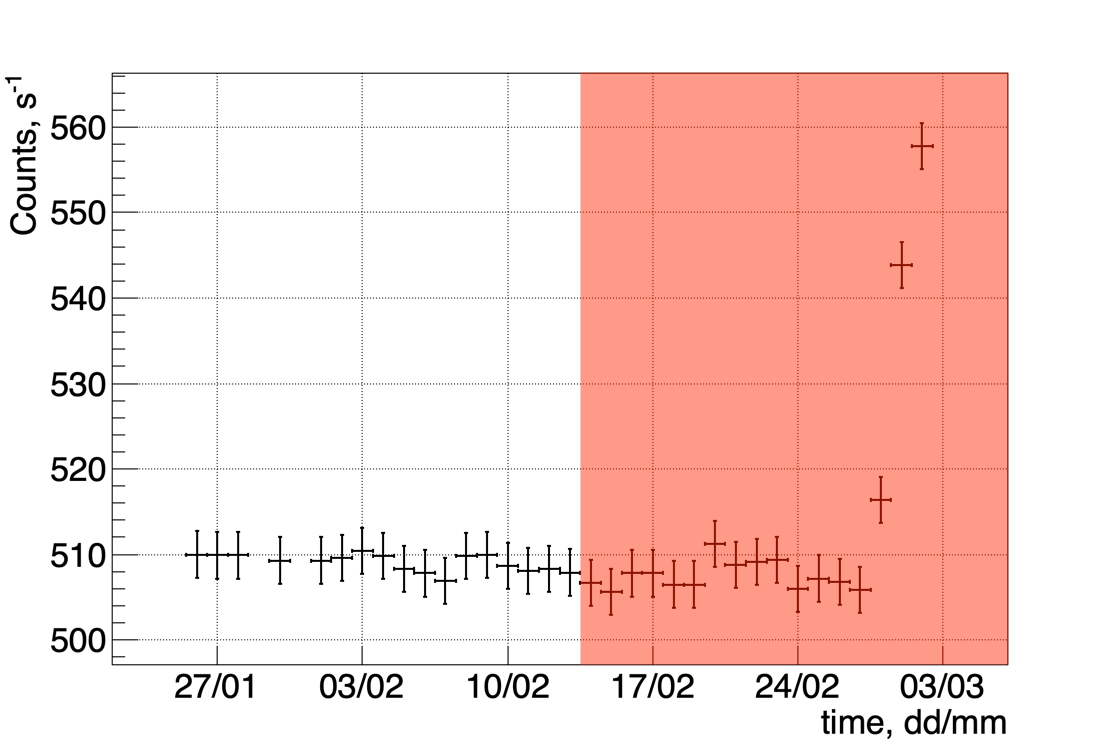
\includegraphics[width=1.0\linewidth]{images/NaI_count_rate_monitoring.png} \\ а)}
  \end{minipage}
  \hfill
  \begin{minipage}[ht]{0.49\linewidth}
    \center{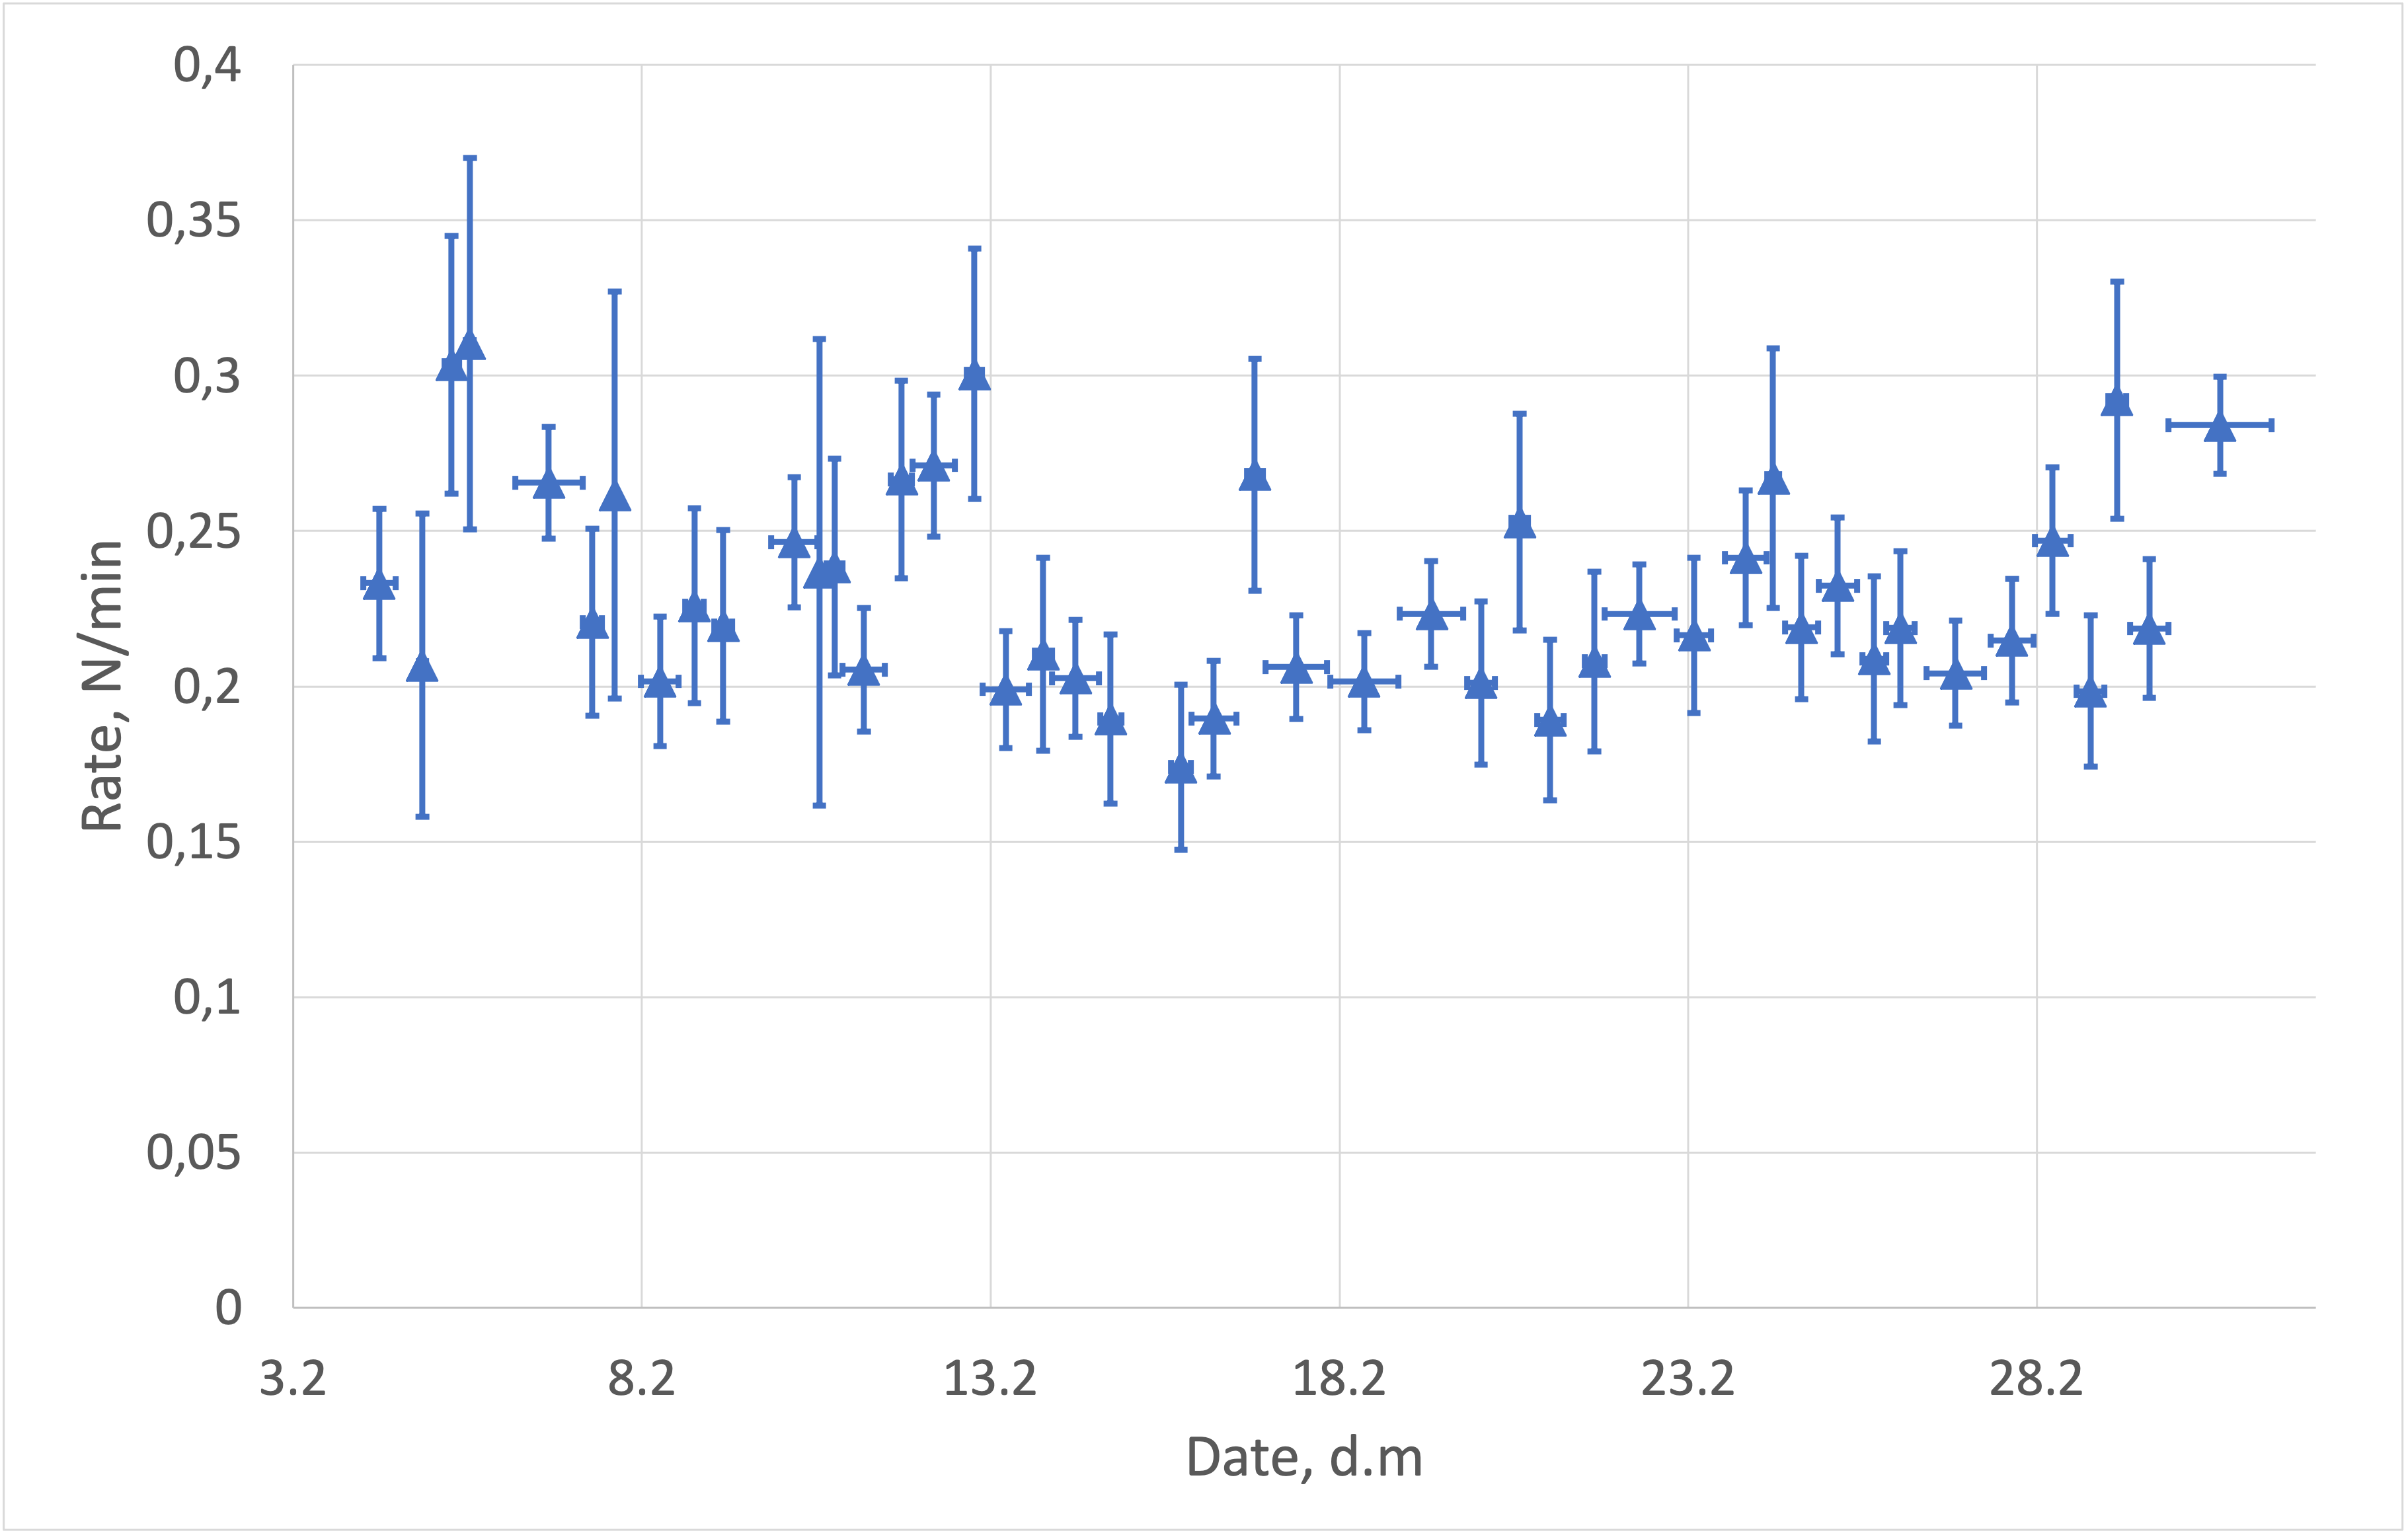
\includegraphics[width=1.0\linewidth]{images/neutrons_rate.png} \\ б)}
  \end{minipage}
  \caption[Графики изменения гамма и нейтронного фонов.]{а) График изменения гамма-фона (измерения суммировались за каждые 3 часа набора данных). б) График изменения нейтронного фона}
  \label{img:gammaneutronbckg}  
\end{figure}

\section{Моделирование отклика детектора РЭД-100}
\label{sect2_3}
Для понимания отклика детектора на различные взаимодействия необходимо детальное моделирование. На данный момент не существует программных пакетов, позволяющих моделировать полную цепь происходящих в детекторе процессов, поэтому было произведено последовательное моделирование в трех различных пакетах. Кроме того, был написан собственный модуль для моделирования временных разверток сигналов.
\subsection{Модель РЭД-100 в различных программных пакетах}
\label{subsect2_3_1}
\textbf{Модель РЭД-100 в GEANT4}
\parРезультат описывающегося теоретическими моделями взаимодействия ионизирующих частиц с веществом моделируется в GEANT4 при помощи методов Монте-Карло~\cite{ALLISON2016186}. GEANT4 — широко используемый в экспериментальной физике программный пакет. GEANT4 предоставляет возможность создания моделей детекторов, состоящих
из различных материалов и использующих различные электрические поля и симулирует поведение частиц в различных частях детектора (например, предоставляя возможность оценить процент отсечения фона защитой). Так же GEANT4 позволяет отслеживать не только конечные частицы, но и промежуточные процессы и их параметры.
\par GEANT4-модель детектора РЭД-100 представляет собой практически полную модель реального детектора. В данном программном пакете происходит моделирование только первичных взаимодействий частицы с рабочим веществом, которое происходит в жидкой фазе. Последующий дрейф электронов в жидкости и газе, а также оптические процессы моделируются с использованием других инструментов.

\par\textbf{Модель РЭД-100 в NEST}
%\label{subsect2_3_2}
\parОсновная функция GEANT — моделирование процессов взаимодействия частиц с материалами, энергопотерь и т.д. Отдельная задача — понимание и моделирование сцинтилляции, ионизации и электролюминесценции. Модуль GEANT-scintillation хоть и позволяет приблизительно оценить численные характеристики данных процессов, но для детального моделирования требуется большая проработанность теоретических моделей и экспериментальных данных. Эту нишу в области моделирования процессов в детекторах на жидких благородных газах занимает NEST. NEST представляет собой программный модуль для предсказания процессов энерговыделения в жидких благородных газах, основанный на совмещении полуэмпирических моделей и экспериментальных данных с разных экспериментов. Более подробно про NEST изложено в кандидатской диссертации Е. Козловой \cite{Kate_thesis}. 
Характеристики детектора РЭД-100, полученные с использованием модели РЭД-100 в NEST:
\begin{enumerate}
    \item Отношение ионизации к сцинтилляции
    \item Количество фотонов электролюминесценции от одного электрона ионизации
    \item Скорость дрейфа электронов в жидкости
\end{enumerate}

\par\textbf{Модель РЭД-100 в ANTS2}
%\label{subsect2_3_3}

ANTS-2 — программный пакет, разработанный для моделирования оптических процессов и обработки данных позиционно-чувствительных детекторов \cite{Morozov_2016}. Также ANTS-2 позволяет задавать оптические свойства материалов и границ между ними, после чего моделировать распространение фотонов от сцинтилляции и электролюминесценции. Плюсом данного пакета является возможность проследить путь каждого фотона от момента возникновения до попадания на фотокатод ФЭУ. 
Кроме того, в данном программном пакете реализованы алгоритмы пространственного восстановления с использованием light response functions (LRFs).
\parВ данном программном пакете была создана детальная оптическая модель детектора РЭД-100, включающая титановый криостат, тефлоновый отражатель, электроды-сетки и кольца-держатели. Данная оптическая модель позволяет проследить путь каждого фотона от рождения до поглощения материалами или регистрацией ФЭУ. 
\subsection{Модель временных разверток}
\label{subsect2_3_2}
Для изучения сигналов в несколько электронов ионизации требуется моделирование временных разверток сигналов электролюминесценции, которые представляют собой раскладку по времени и каналам регистрации для всех зарегистрированных фотонов. 
\parЭлектроны ионизации после возникновения дрейфуют к границе раздела фаз, при это подвергаясь диффузии как по оси Z, так и в плоскости XY. Диффузия описывается следующим образом \cite{EXO-200:2016qyl}:
\begin{equation}
n(\vec{x}, t)=\frac{N}{4 \pi D_T t \sqrt{4 \pi D_L t}} \exp \left[\frac{-\left(x^2+y^2\right)}{4 D_T t}\right] \times \exp \left[\frac{-\left(z-v_d t\right)^2}{4 D_L t}\right]
\label{diffusion}
\end{equation}
\par Параметр $D_L$ в данном случае был принят равным $25 см^2$/c \cite{Njoya:2019ldm}.
Диффузия в плоскости XY не учитывалась, так при прохождении через электроды-сетки электроны концентрируются в центрах ячеек, размер которых сильно превышает масштаб диффузии на рассматриваемой глубине.
\par Сигнал от одиночного электрона ионизации моделируется следующим образом:
\begin{enumerate}
    \item Для точек, расположенных в центрах ячеек электрода-сетки рассчитывается относительная вероятность для каждого ФЭУ зарегистрировать фотон, испущенный из этой точки. В данном случае используется приближение о том, что все фотоны электролюминесценции испускаются из одной точки. 
    \item Для каждого фотона в соответствии с равномерным разыгрывается координата испускания внутри электролюминесцентного зазора.
    \item Количество фотонов разыгрывается в соответствии с распределением Гаусса, парметры которого подбираются таким образом чтобы (в конце концов все сошлось) среднее значение которого рассчитывается исходя из экспериментального распределения суммарного светосбора в центре детектора и отношения суммарной относительной вероятности в конкретной точке к соответствуеющему значению в центре детектора. (с учетом положения). Среднеквадратичное отклонение складывается из Пуассоновского размытия и дополнительной компоненты неизвестной природы.
    \item Истинная длительность события (непосредственно время дрейфа электрона через электролюминесцентный зазор) разыгрывается в соответствии с распределением Гаусса с параметрами, подобранными экспериментально. 
    \item Исходя из истинной длительности события, координаты испускания фотонов, полученные на шаге 2, пересчитываются во времена испускания. Так как скорость света на данных масштабах расстояний можно считать достаточно большой, времена испускания соответствуют временам регистрации фотонов.
\end{enumerate}

Для создания сигналов от нескольких электронов ионизации требуется скомбинировать несколько событий от одного электрона ионизации. При этом время начала электролюминесценции для каждого SE размывается в соответствии с формулой \ref{diffusion} и скоростью дрейфа в жидкости, рассчитанной при помощи пакета NEST. Реализация описанной в данном разделе симуляции написана автором на языке python 3.8. Пример визуализации смоделированного описанным выше способом события представлен на рисунке~\ref{img:simulationevent}

\begin{figure}[H]
  \center{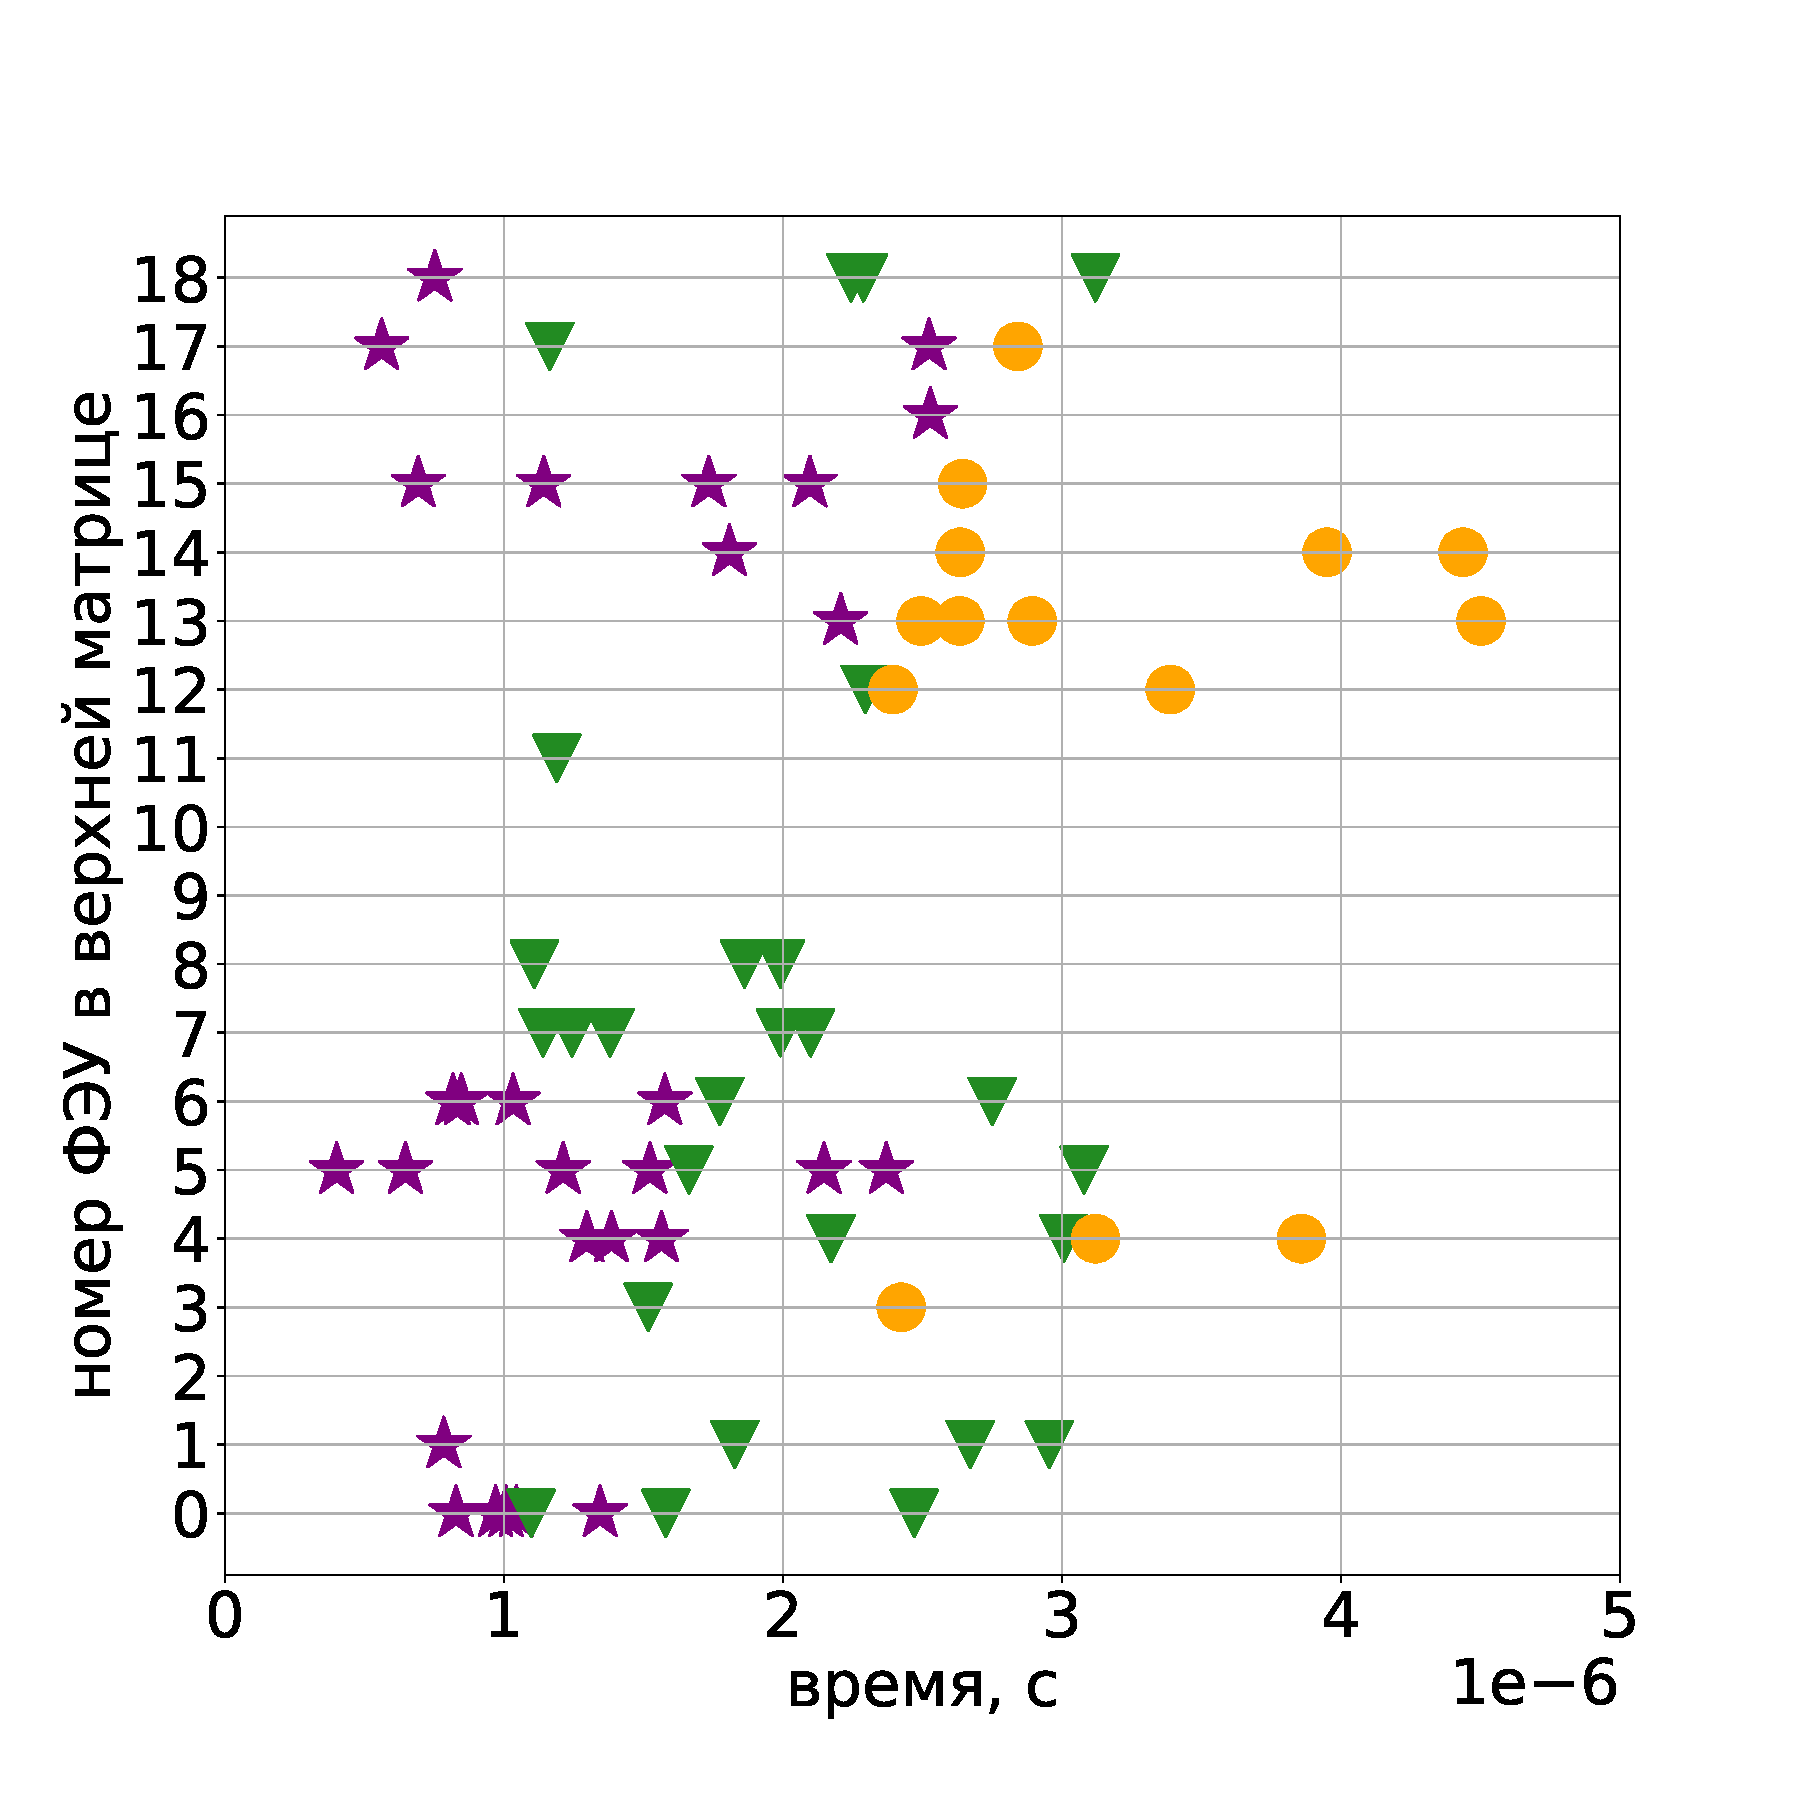
\includegraphics[width=0.6\linewidth]{images/simulation_event_example.pdf}}
  \caption[Пример смоделированного с использованием LRF из оптической модели события в 3 SE.] {Пример смоделированного с использованием LRF из оптической модели события в 3 SE. Различными цветами (значками) обозначены фотоны, возникшие от разных электронов ионизации.}
  \label{img:simulationevent}  
\end{figure}           % Глава 2
\chapter{Анализ калибровочных данных РЭД-100} 
\label{chapt3}

\section{Калибровка мюонами}
\label{sect3_1}
Как уже было сказано ранее, при дрейфе в ксеноне электроны ионизации претерпевают потери, связанные с захватом их примесями. Как известно, процесс таких потерь описывается экспоненциальной функцией. Для измерения времени жизни мюонные сигналы, записанные в специальном режиме работы детектора (см.~\ref{muons}), фитировались функцией $ f(t) = A\cdot exp(-\frac{t}{\tau})$, где $\tau$ -- среднее времени
жизни электронов до захвата $\tau$, за которое количество дрейфующих электронов ионизации уменьшается в e раз. Пример усредненного сигнала и его фитирования приведен на рисунке \ref{img:muonsignal}. Усреднение сигнала проводилось путем суммирования большого количества одиночных сигналов.
\begin{figure}[H]	\center{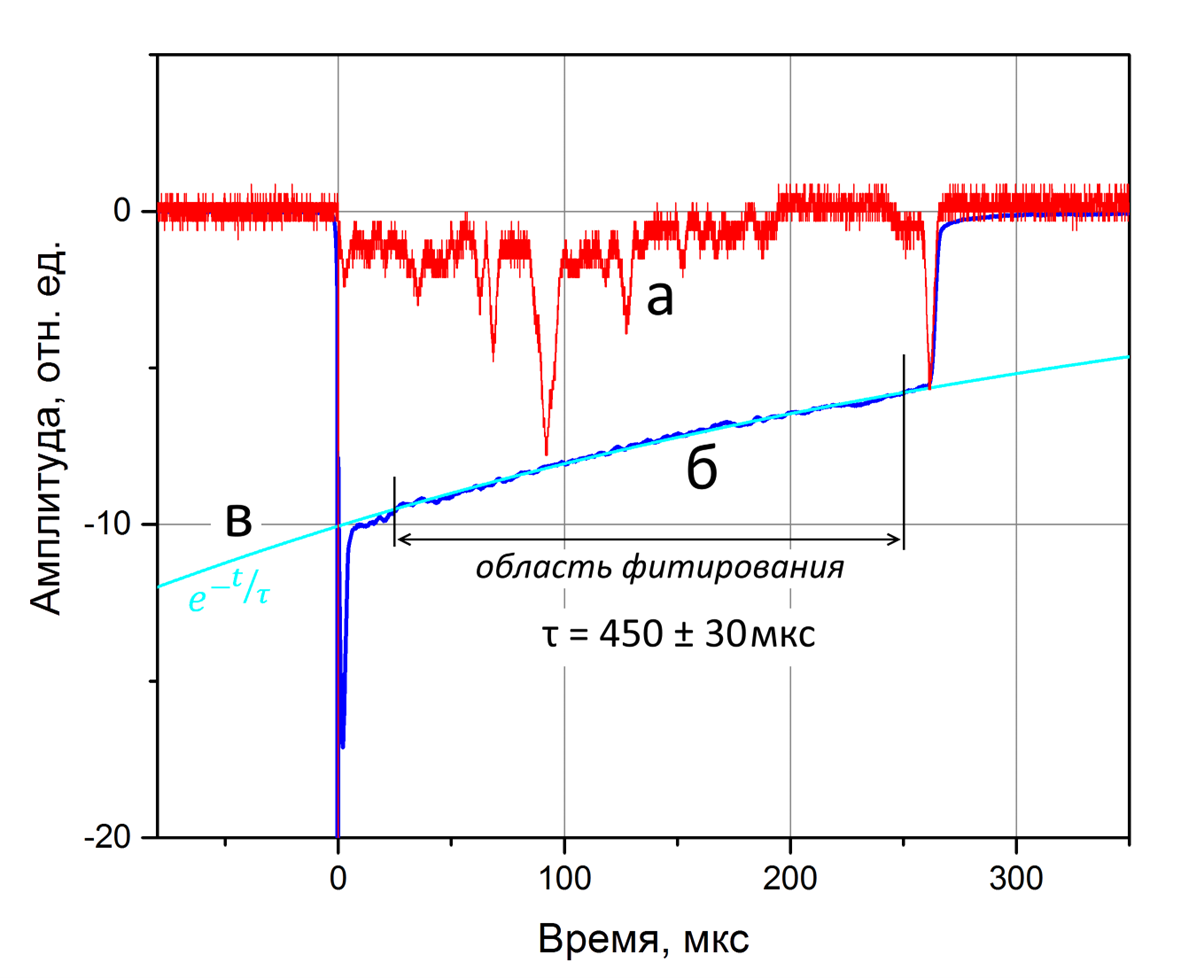
\includegraphics[width=0.8\linewidth]{images/Graph41_labels.png}}
	\caption[Пример определения времени жизни электронов ионизации до захвата электроотрицательными примесями в жидком ксеноне.]{а) — типичный мюонный сигнал, б) — сигнал, усреднённый по 10 000 событий, в — экспоненциально спадающая функция, аппроксимирующая «ступеньку» усреднённого сигнала.}
	\label{img:muonsignal}
\end{figure}

Эволюция времени жизни в течение сеанса показана
на рисунках \ref{img:lt2019}, \ref{img:lt2022}

\begin{figure}[H]	\center{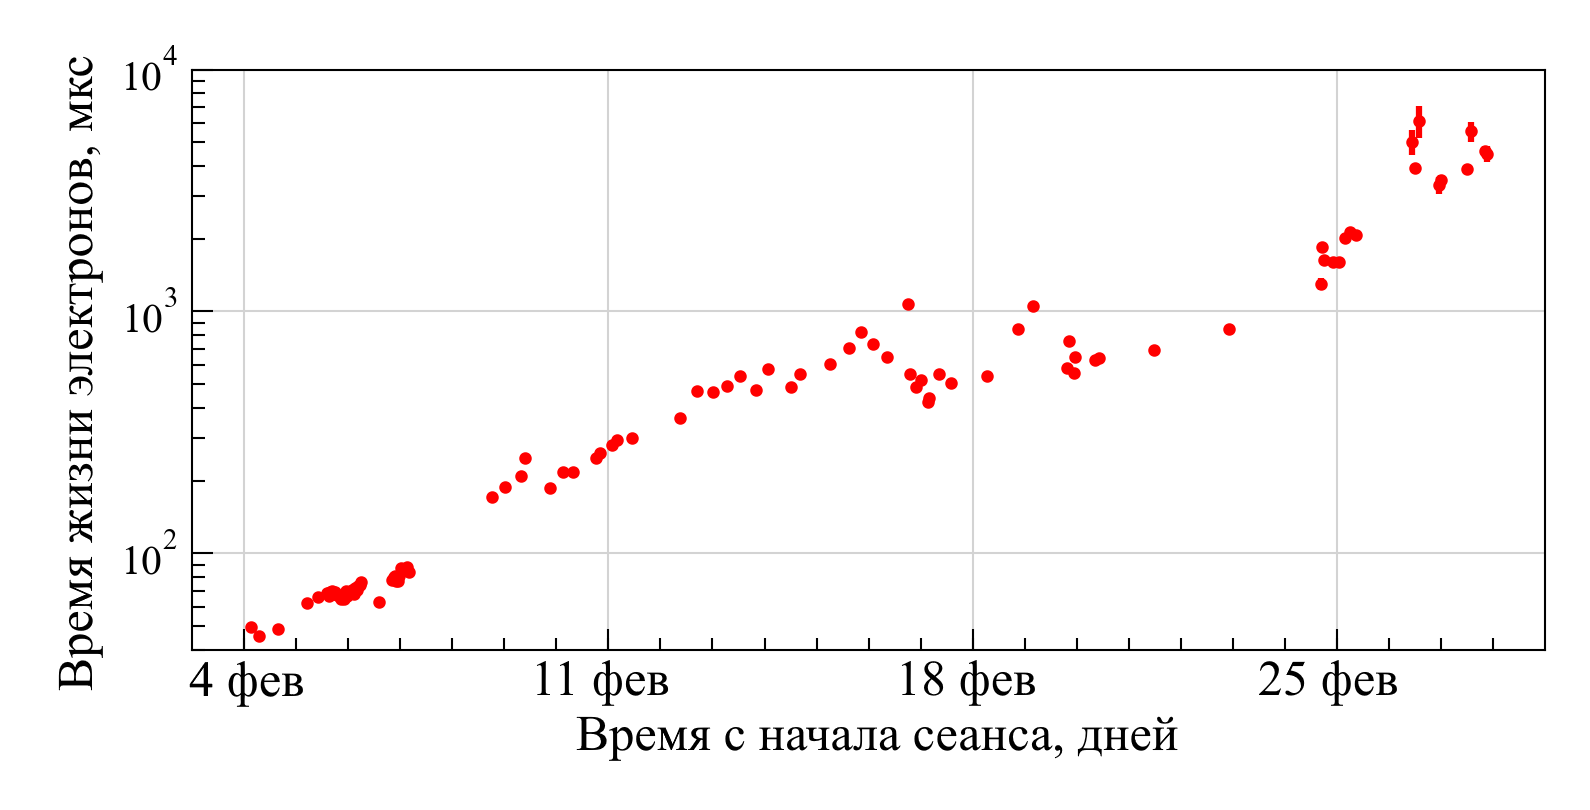
\includegraphics[width=0.8\linewidth]{images/RED100. Graph. e_lifetime_2019_published_RU.png}}
	\caption{Динамика изменения времени жизни электронов в детекторе РЭД-100 в течение инженерного сеанса 2019 года}
	\label{img:lt2019}
\end{figure}

\begin{figure}[H]	\center{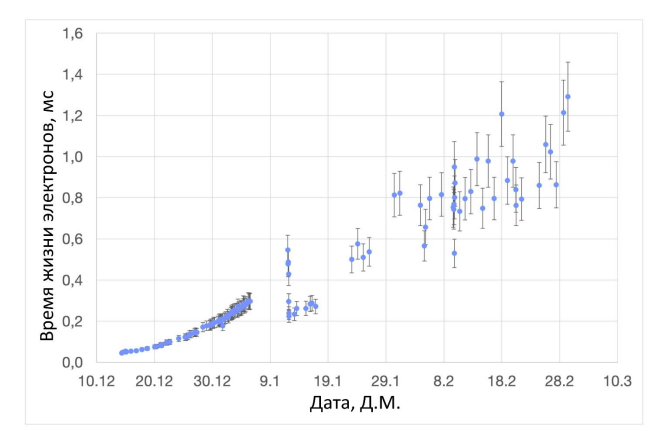
\includegraphics[width=0.8\linewidth]{images/lifetime2022.png}}
	\caption{Динамика изменения времени жизни электронов в детекторе РЭД-100 в течение сеанса на КАЭС 2022 года}
	\label{img:lt2022}
\end{figure}

%Как вы можете видеть, достигнута хорошая чистота, которая соответствует на полной длине дрейфа не больше чем ... (процент от сигнала).
%+ мб про концентрацию? (Леше задать вопрос)

\section{LED-калибровка}
\label{sect3_2}
После обработки данных пакетом REDOffline, из обнаруженных импульсов отбирались импульсы с амплитудой и длительностью больше пороговых, которые представлены в таблице \ref{tab:spethresholds}.
\begin{table}[hbt]
    \centering
        \caption{Пороговые значения для отбора импульсов с целью получения спектров SPE сигналов.}
\begin{tabular}{|c|c|c|}
\hline
    Сеанс & Амплитуда & Длительность\\
    \hline
    2019 & 1.5 мВ & 4 нс\\
    \hline
    2021-22 & 2 мВ & 4 нс\\
    \hline
\end{tabular}
    \label{tab:spethresholds}
\end{table}

Характерные значения зарядов однофотоэлектронных сигналов ФЭУ были получены на основе фитирования спектров площадей отобранных импульсов следующей функцией:
%переназвать N ()
\begin{equation}
N=\exp (a+k Q)+c \cdot \exp \left(-\frac{\left(Q-Q_0\right)^2}{2 \sigma^2}\right)
\label{spefitfunc}
\end{equation}
\par В данной формуле $Q$ - площадь (заряд) импульса ФЭУ,  Экспоненциальное слагаемое в данном случае соответствует шумовой части спектра, а распределение Гаусса -- непосредственно спектру однофотоэлектронных сигналов. Результат 2019 года показал, что интересующий нас сигнал отстоит достаточно далеко от шумов электроники, поэтому при анализе данных, набранных на КАЭС фитирование производилось только распределением Гаусса. Примеры фитированных спектров представлены на рисунке \ref{img:spe2019} для 2019 года и на рисунке \ref{img:spe2022} для 2021-22. 

\begin{figure}[H]
	\center{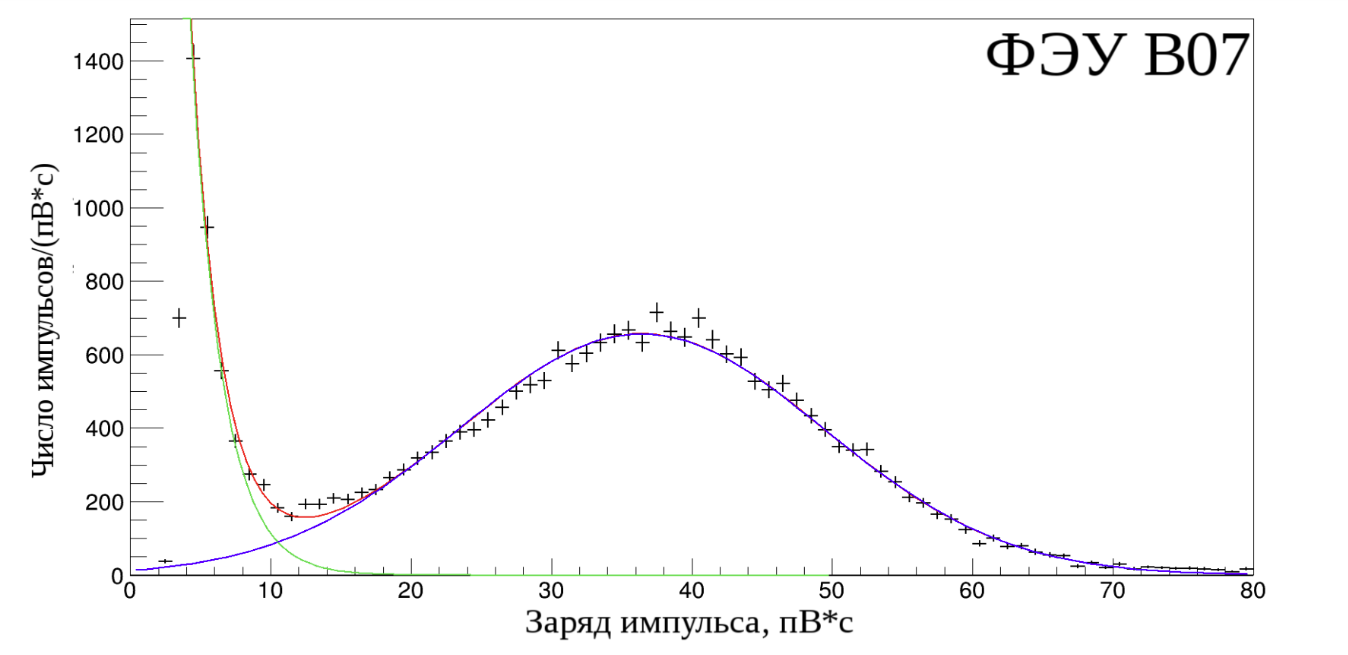
\includegraphics[width=0.8\linewidth]{images/SPE_spectrum.png}}
	\caption[Спектр площадей импульсов для ФЭУ В07(из нижней матрицы) и результат его фитирования функцией \ref{spefitfunc}) для инженерного запуска РЭД-100.] {Спектр площадей импульсов для ФЭУ В07(из нижней матрицы) и результат его фитирования функцией \ref{spefitfunc}) для инженерного запуска РЭД-100. Синим обозначена часть, соответствующая нормальному распределению, зеленым -- часть, соответствующая экспоненциальной функции, красным -- их сумма.}
	\label{img:spe2019}
\end{figure}

\begin{figure}[H]
	\center{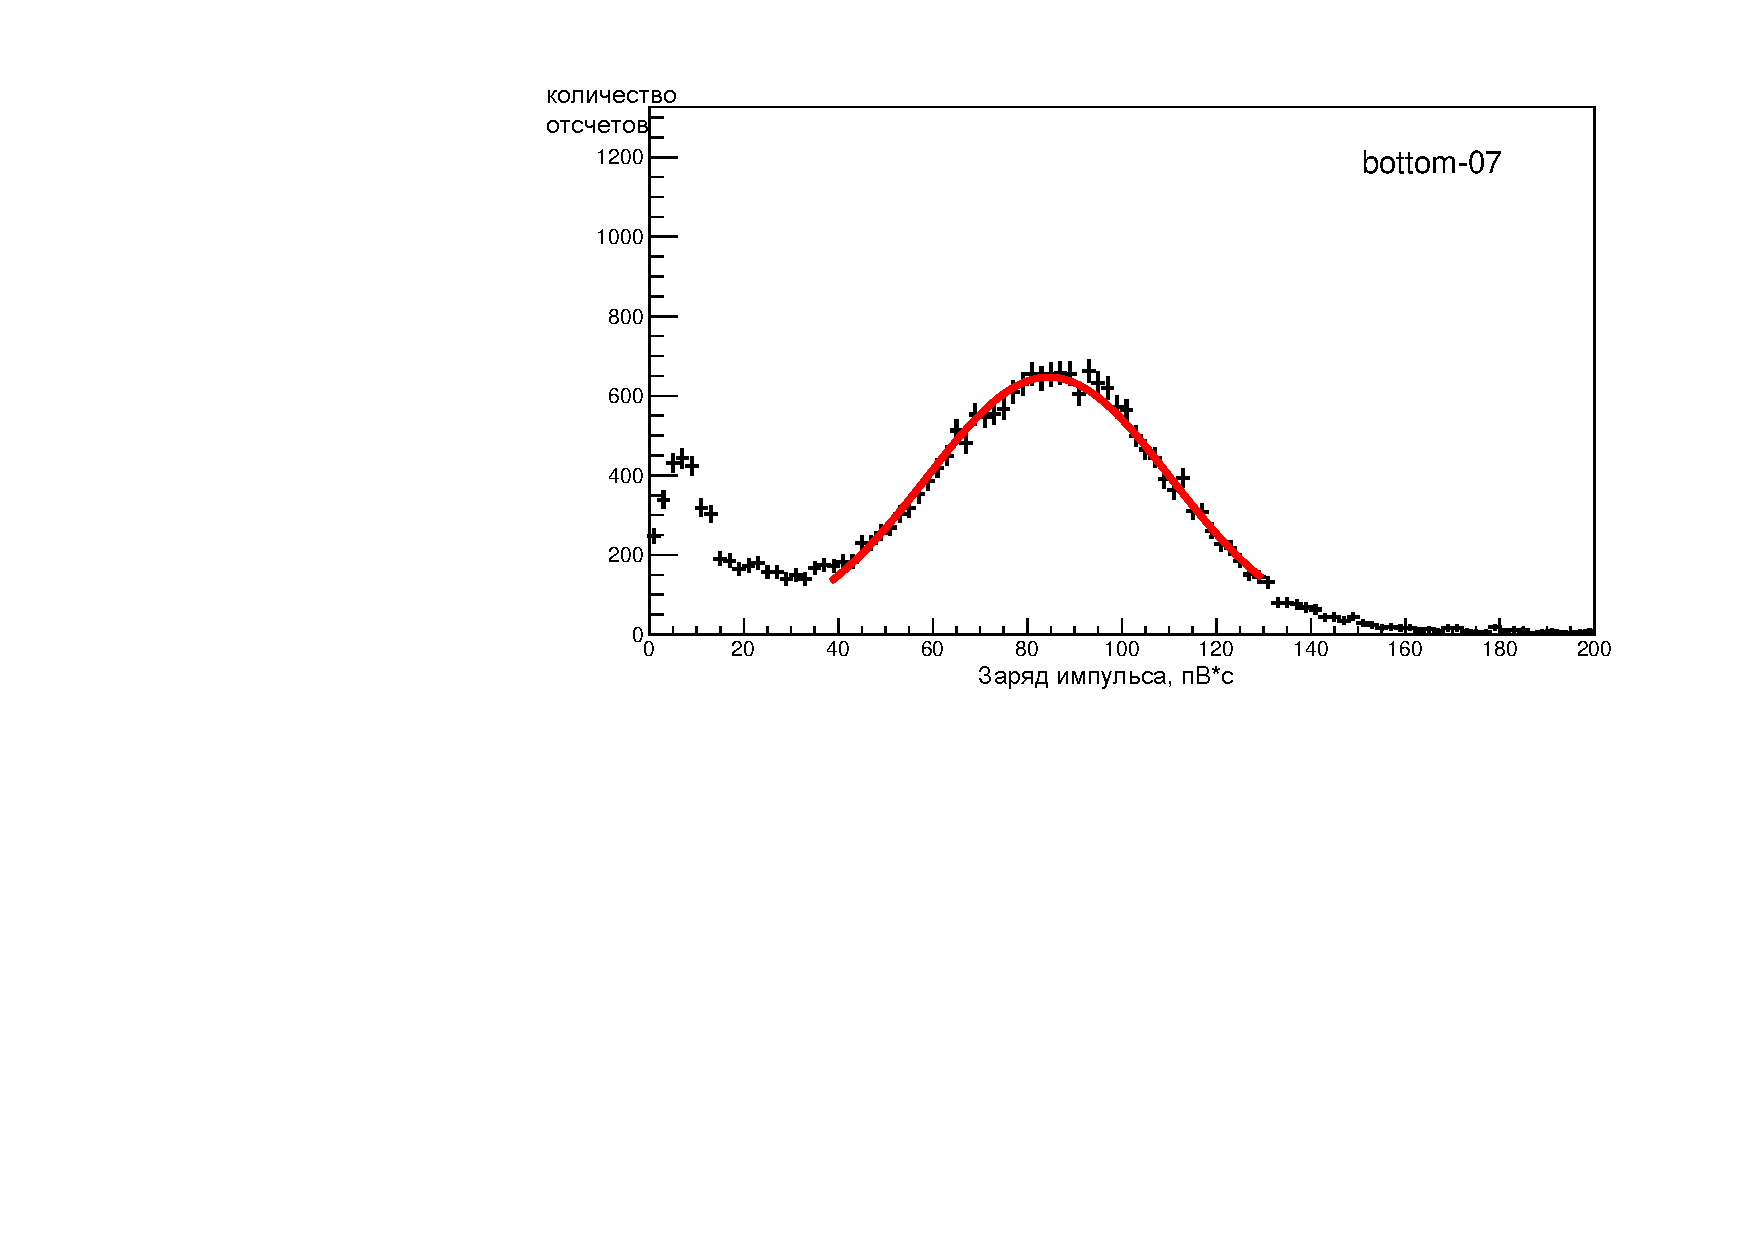
\includegraphics[width=0.8\linewidth]{images/ledspectrum2022.pdf}}
	\caption[Спектр площадей импульсов для ФЭУ В07(из нижней матрицы) и результат его фитирования распределением Гаусса для эксперимента на КАЭС.]{Спектр площадей импульсов для нескольких ФЭУ и результат фитирования распределением Гаусса для эксперимента на КАЭС. Красной линией обозначен результат фитирования.}
	\label{img:spe2022}
\end{figure}

Результаты SPE-калибровок с использованием светодиода для инженерного сеанса и сеанса на КАЭС для всех ФЭУ приведены в таблицах в~\ref{AppendixA1}. Существенное (более чем в два раза) отличие характерных зарядов SPE для двух сеансов связано с изменением рабочего напряжения на ФЭУ. 

Сеанс набора данных на КАЭС был существенно дольше, чем инженерный ран в МИФИ, поэтому требовался более тщательный анализ SPE-калибровок. Для дополнительной проверки помимо импульсов из данных, набранных со светодиодом, были отобраны одиночные импульсы на формах сигналов от SE-калибровок, а также на формах сигналов с УКРН-подобными событиями. Пример сравнения полученных положений SPE пика представлен на рисунке \ref{img:spevstime2022}. 

\begin{figure}[H]
	\center{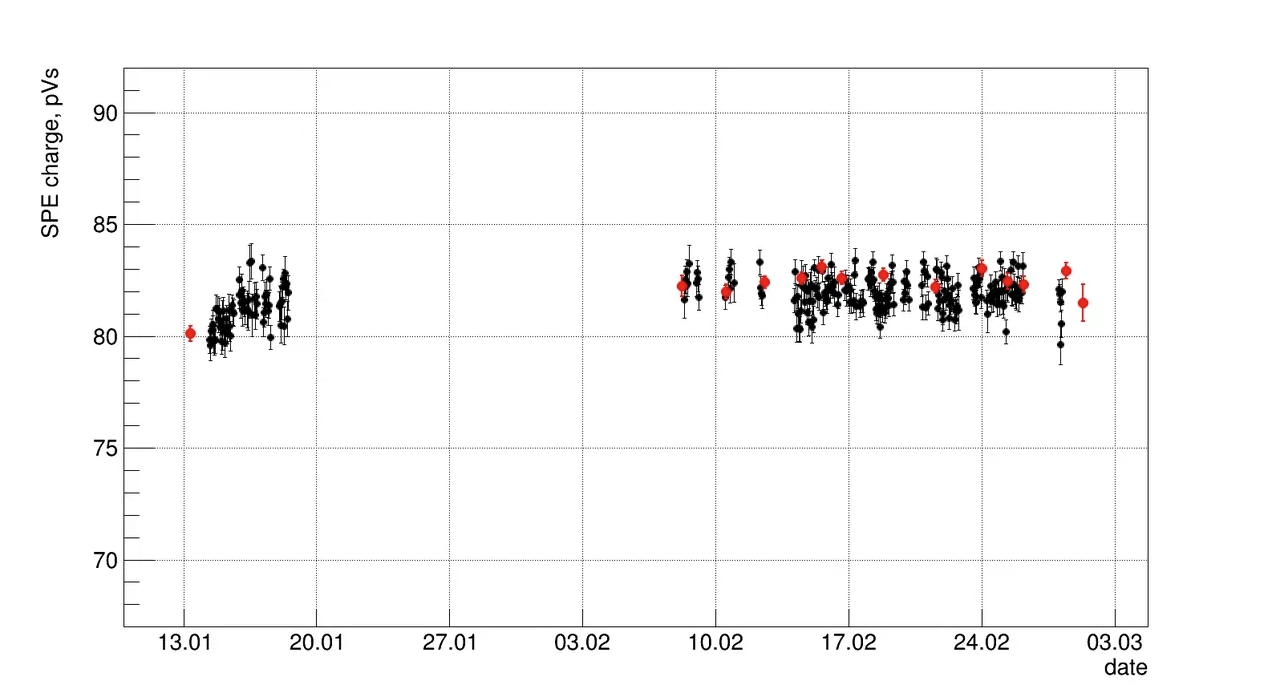
\includegraphics[width=0.8\linewidth]{images/spevstime2022.png}}
	\caption[Пример зависимости положения SPE-пика, полученного разными способами, от времени.] {Пример зависимости положения SPE-пика, полученного разными способами, от времени. Черным обозначены измерения при помощи SE калибровок, красным -- при помощи LED калибровок. Промежуток в наборе данных связан с техническими неполадками.}
	\label{img:spevstime2022}
\end{figure}

Кроме того, так как сеанс набора данных был длительный, была обнаружена слабая зависимость величины SPE импульсов от времени. Она связана с изменением параметров детектора и электроники. Так как измерения на КАЭС требовали повышенной точности, данная зависимость была учтена путем фитирования зависимости данных SPE-калибровок кусочно-линейной функцией. Пример такого фитирования показан на рисунке~\ref{img:spevstimefit}.

\begin{figure}[H]
	\center{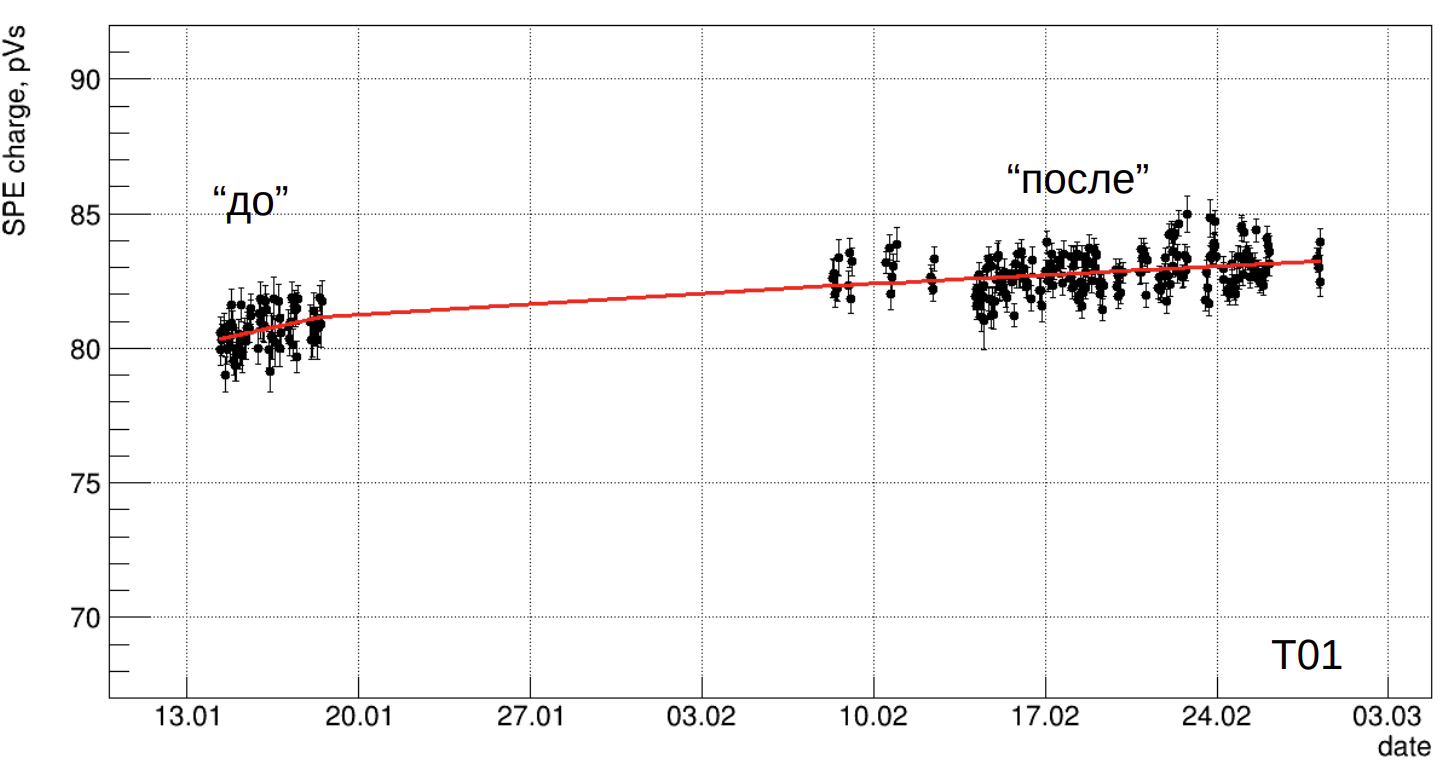
\includegraphics[width=0.8\linewidth]{images/spevstimefit.png}}
	\caption[Пример фитирования зависимости положения SPE пика от времени для ФЭУ Т01.] {Пример фитирования зависимости положения SPE пика от времени кусочно-линейной функцией для ФЭУ Т01. Промежуток в наборе данных связан с техническими неполадками.}
	\label{img:spevstimefit}
\end{figure}

\section{Калибровка гамма-источниками}
\label{sect3_3}
Обработка LED-калибровок предполагает анализ одиночных форм сигналов и выделение на них импульсов соответствующих определенным параметрам. Обработка измерений с гамма-источниками принципиально отличается, так как требует выделений событий, которые которые представляют собой совпадение по времени импульсов во многих каналах и анализа сигналов с разных каналов в комплексе. Для этой цели была разработана цепочка алгоритмов, изложенная в данном разделе.
\subsection{Кластеризация}
\label{subsect3_3_1}
Гамма-кванты дают световыход в детекторе, достаточно большой для того, чтобы в каждом ФЭУ был ощутимый световой сигнал. Поэтому для анализа применяется суммарная форма сигнала, в которой импульсы от физических сигналов в разных ФЭУ будут складываться, а совпадений случайных импульсов с таковыми в других ФЭУ не будет.

После обработки сырых форм сигналов при помощи RED-offline требовалось выделить на них кластеры -- группы импульсов, соответствующие сигналам от сцинтилляции и электролюминесценции. Для ускорения процесса обработки был реализован следующий алгоритм:
\begin{enumerate}
    \item Формировались прямоугольные импульсы, длительность которых была равна длительности оригинального импульса, а высота определялась как отношение площади оригинального импульса к его длительности
    \item Полученные прямоугольные импульсы со всех каналов складывались в одну суммарную псевдо-форму сигнала
    \item На полученной псевдо-форме сигнала проводился поиск импульсов, соответствующих S1 и S2 по следующим критериям:
    \begin{itemize}
        \item S1: длительность от 70 нс до 170 нс; амплитуда от 0.4e-6 В до 1.8e-6 В 
        \item S2: длительность больше 1800 нс; по амплитуде дополнительных отборов не применялось.
    \end{itemize}
\end{enumerate}
Из оригинальных импульсов, содержащихся в отобранных кластерах, формировались калибровочные события. Площадь каждого сигнала S2 была скорректирована в соответствии с временем жизни электронов в жидком ксеноне. Также площади, изначально определенные в В$\cdot$с, были поделены на площади единичного SPE для каждого ФЭУ. 
Также был произведен переход от измерения площадей в В$\cdot$с к измерению в единицых SPE, что позволило избавиться от эффектов зависимости SPE-калибровок от времени и номера канала.

Для дальнейшего анализа был применен дополнительный отбор на количество S1 и S2 -- каждое событие должно было содержать ровно одну вспышку S1 и одну S2. Данный отбор необходим для более чистого разделения событий и выделения калибровочных пиков.

\subsection{Пространственное восстановление}
\label{subsect3_3_2}
Наиболее простым способом получения координат событий является центроид, который состоит в том, что координата вспышки находится по формуле~\cite{6154607}:
\begin{equation}
    X_{event} = \frac{\sum\limits_{i}A_iX_i}{\sum\limits_{i}A_i},
\end{equation}
где $X_i$, $A_i$ --- координаты и сигналы ФЭУ в данном событии. Энергия в данном случае может быть восстановлена как простая сумма сигналов. Здесь и далее под сигналом ФЭУ понимается площадь импульсов. Однако, данный метод позволяет эффективно восстанавливать координаты событий только в непосредственной близости от центра детектора. События, которые произошли по краям рабочего объема, при восстановлении центроидом стягиваются ближе к центру (рисунок \ref{ris:basecen}), так как сигнал с центральных ФЭУ ничем не компенсируется для краевых событий. Несомненным плюсом восстановления методом центроида является отсутствие необходимости в каких-либо других данных и расчетах кроме откликов ФЭУ и их координат.
\begin{figure}[hbt]
	\center{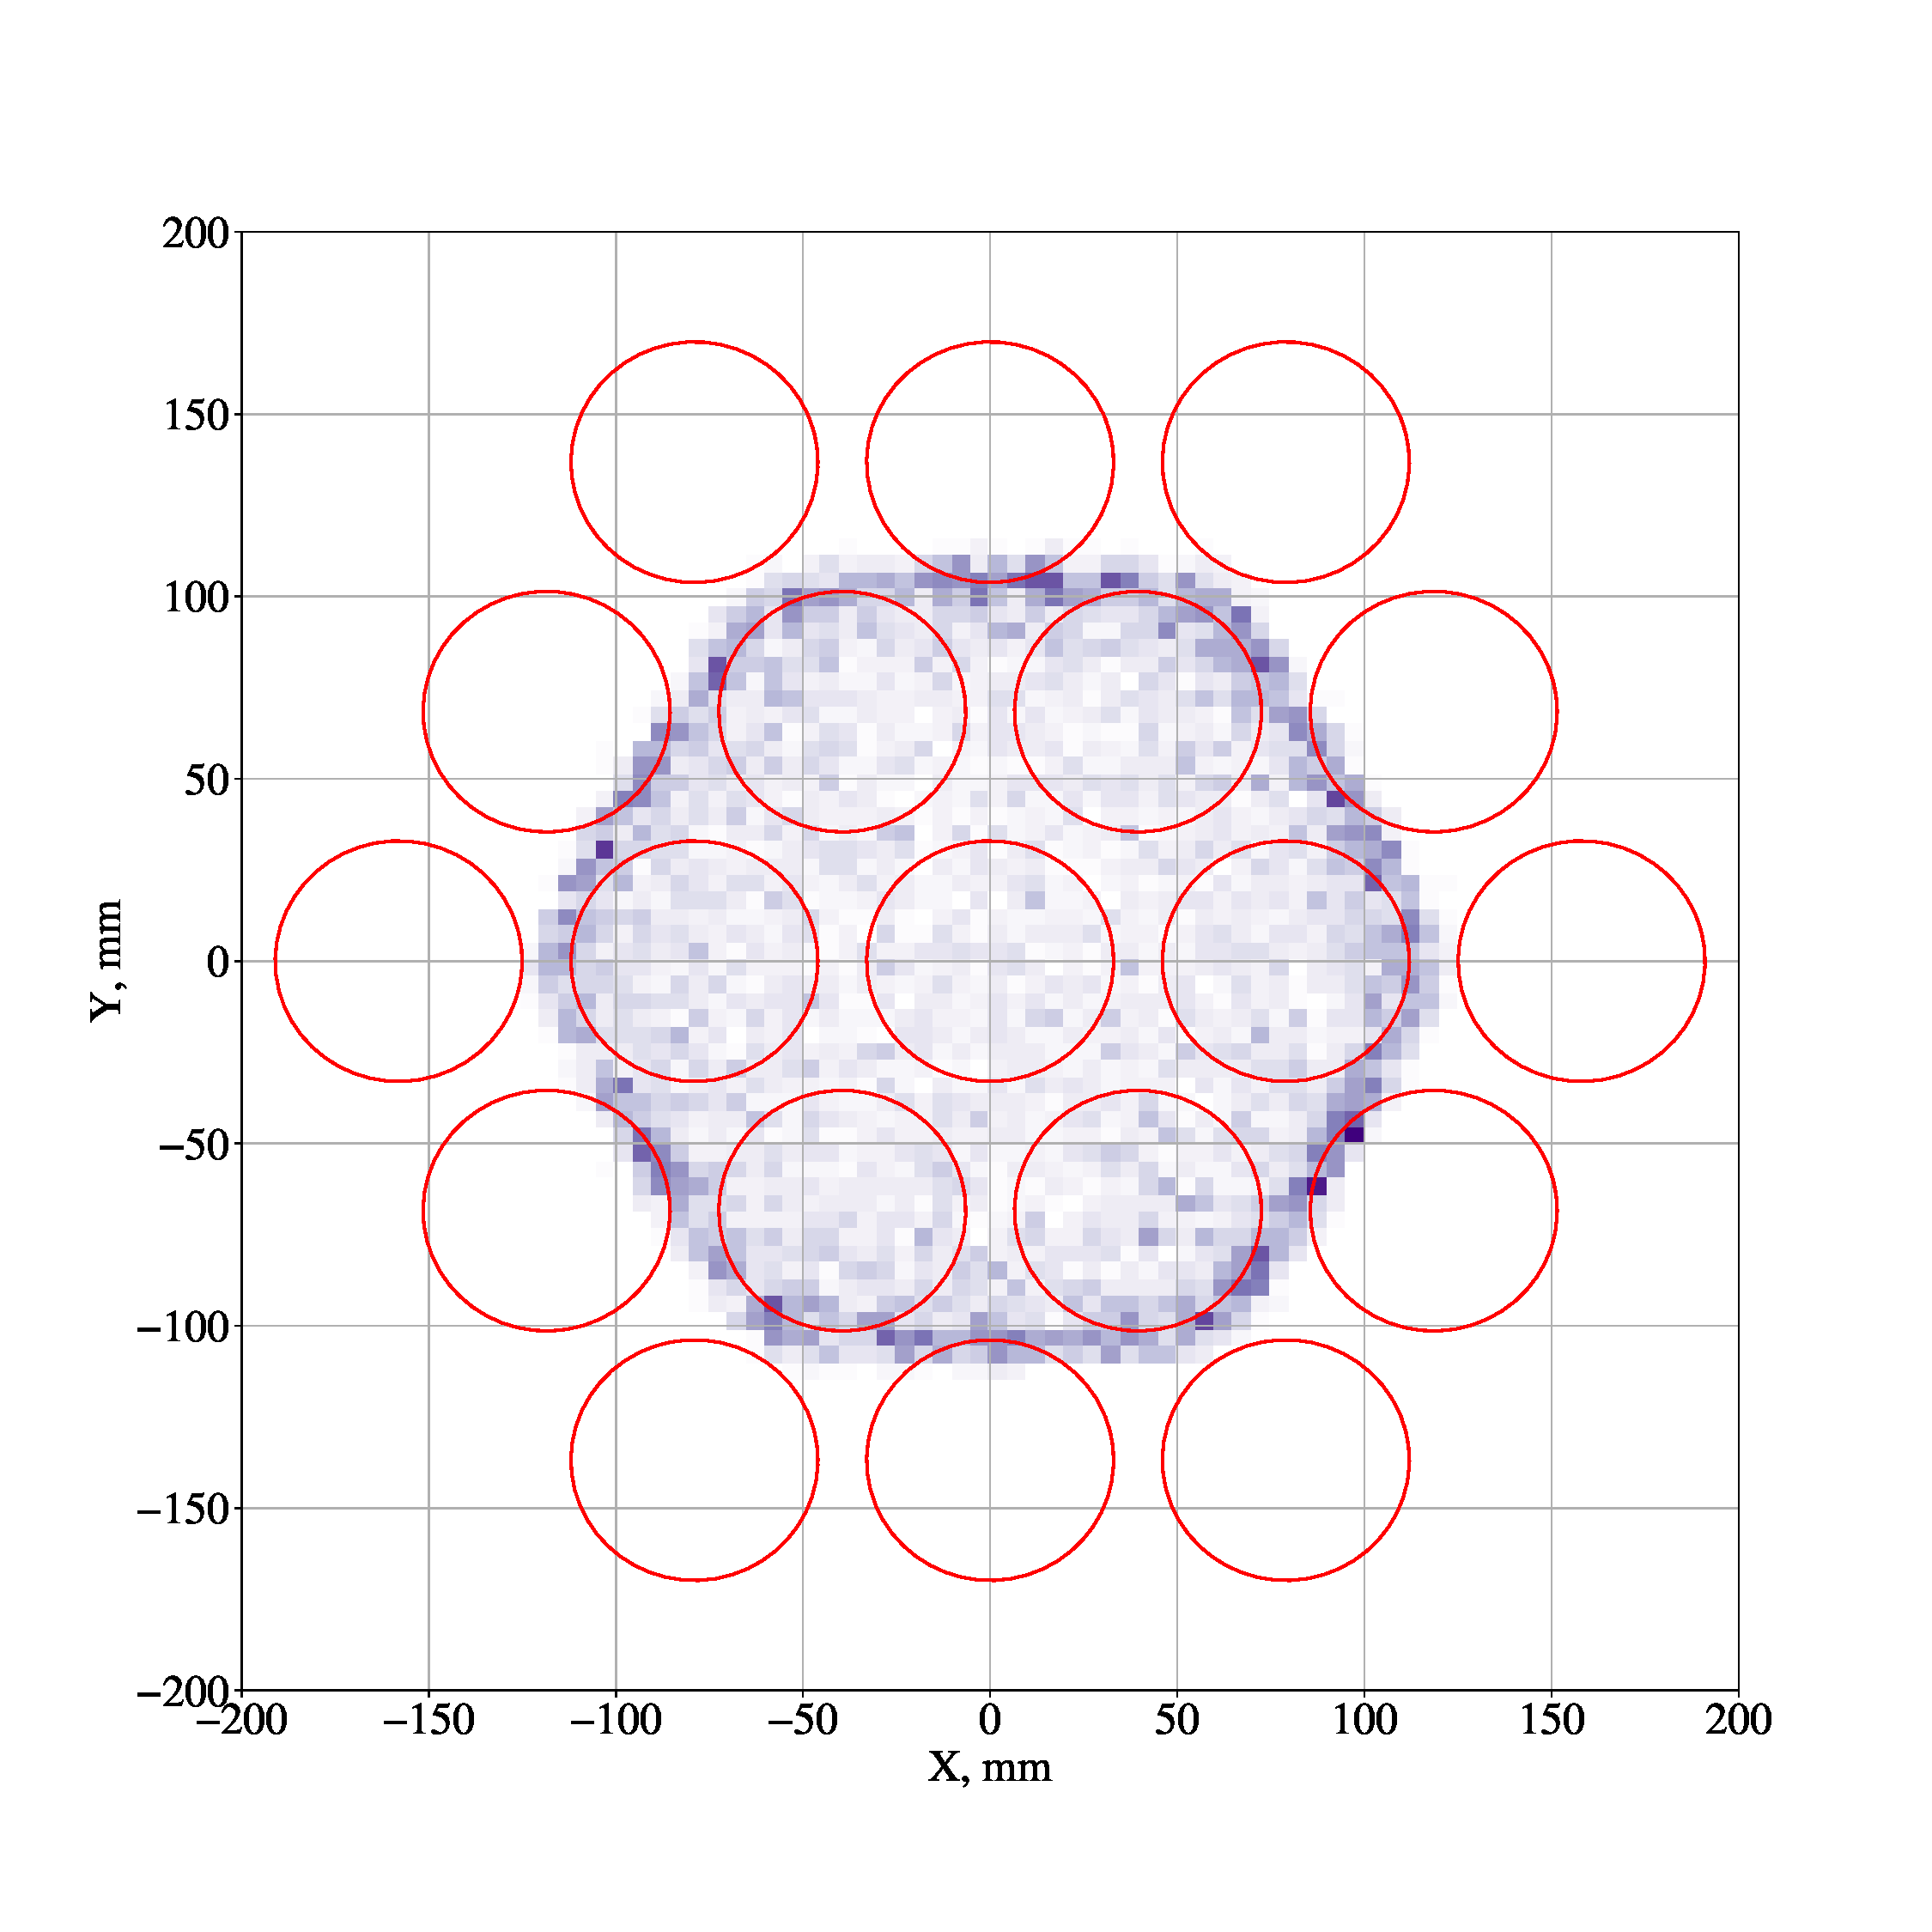
\includegraphics[width=0.8\linewidth]{images/basecentro.pdf}}
	\caption{Распределение восстановленных смоделированных событий методом нескорректированного центроида. Красными окружностями обозначены ФЭУ.}
	\label{ris:basecen}
\end{figure}
%развернуть этот график
\begin{figure}[hbt]
	\center{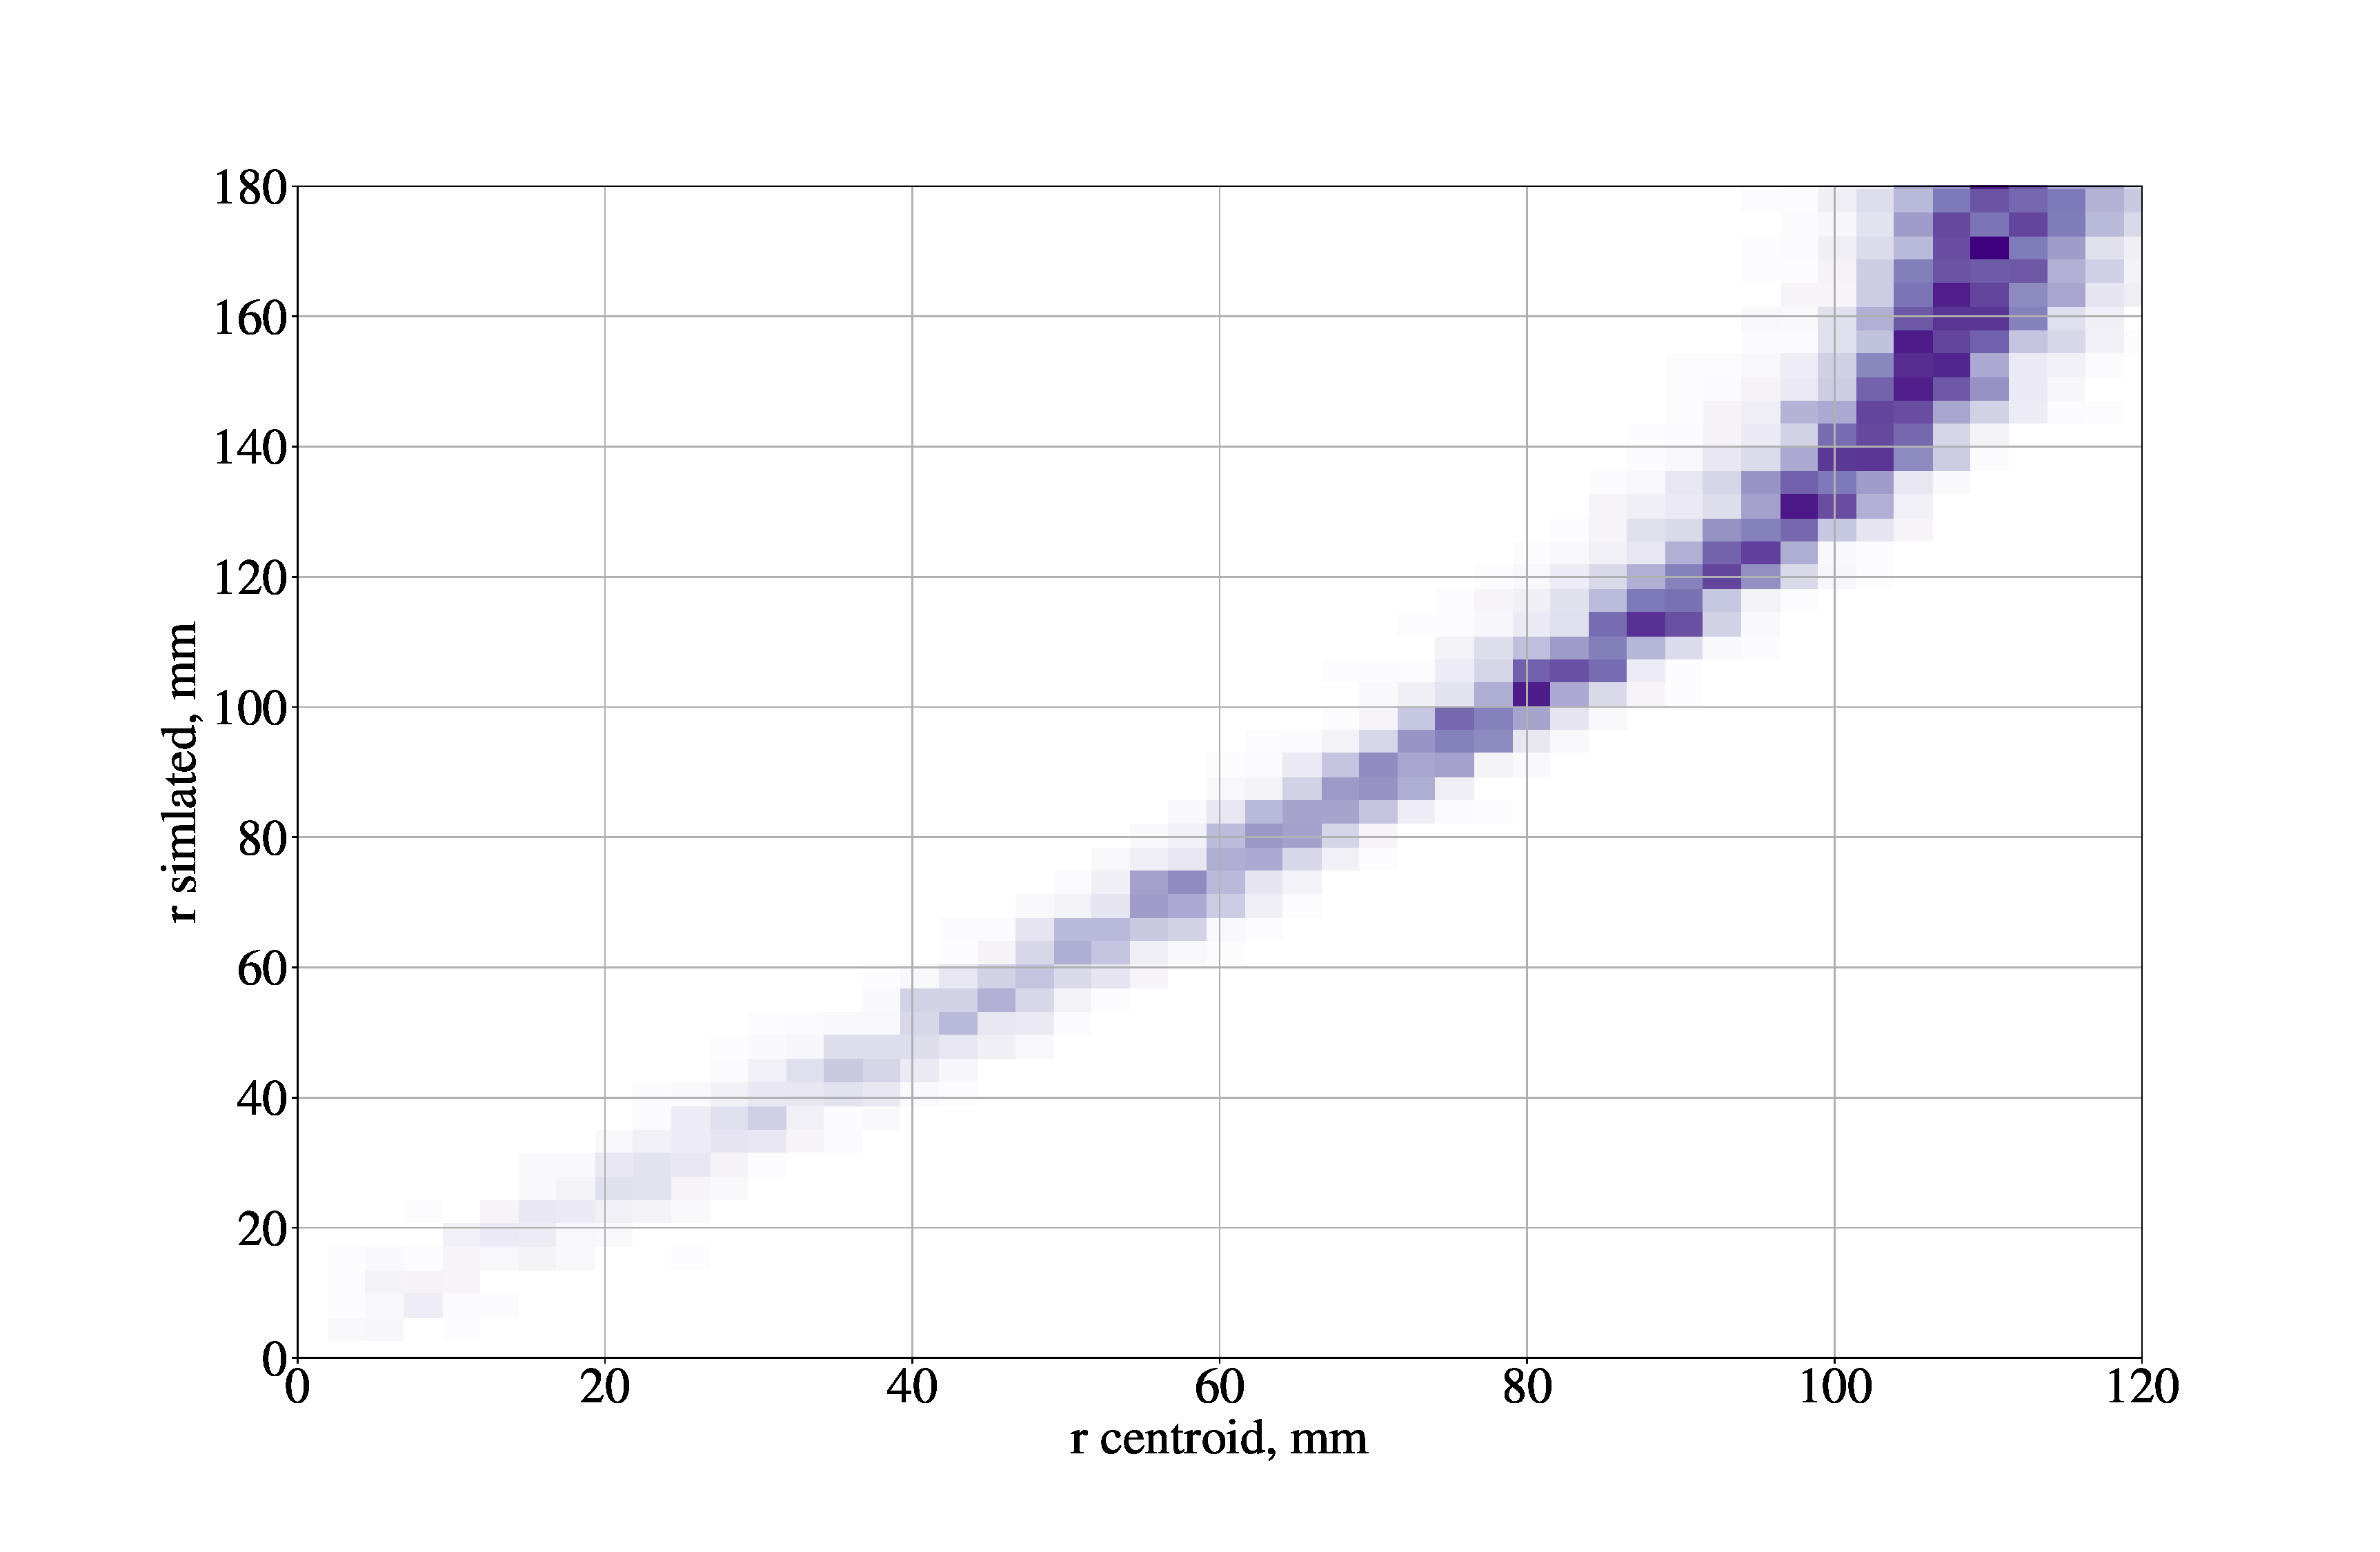
\includegraphics[width=1\linewidth]{images/rvsr.pdf}}
	\caption{Зависимость радиуса для смоделированных событий от радиуса, полученного в результате восстановления методом центроида}
	\label{ris:rvsr}
\end{figure}
\parИдея многих других методов пространственного восстановления заключается в построении функций эффективности светосбора (light response functions --- LRF) для каждого ФЭУ, которая представляет собой зависимость отклика ФЭУ от положения источника света. Эти методы опираются на предположение, что форма LRF не зависит от количества света, что с высокой степенью надежности выполняется в большинстве случаев. Формы LRF могут быть получены разными способами, как аналитическим расчетом, так и в результате моделирования или анализа экспериментальных данных, а также комбинацией этих способов. Наиболее простой метод, основанный на использовании LRF --- скорректированный центроид. В данном случае удобнее использовать полярные координаты $r$ и $\varphi$. На рисунке~\ref{ris:rvsr} приведена зависимость полярного радиуса для некоторых смоделированных событий от радиуса, полученного в результате восстановления координат этих событий методом центроида. С использованием данной зависимости производится поиск функции $r_{corrcentr} = f(r_{centr}, \varphi)$, где $r_{corrcentr}$, $r_{centr}$ --- скорректированный и нескорректированный радиус.  Искажения полярного угла $\varphi$ обычно малы и его коррекция может не производиться. Для детектора РЭД-100 один из вариантов вида функции $f$, определенный эмпирическим путем, выглядит следующим образом:
\begin{equation}
   f(r_{centr}, \varphi) = \Big(A\cdot r_{centr}^2+B\cdot r_{centr}\Big)\cdot\Big( 1-C\cdot \exp(D\cdot r_{centr})\cdot(\cos 6\varphi)\Big),
\end{equation}
где $A, B, C, D$ --- параметры, вычисляемые исходя из имеющихся LRF. Данный метод не обеспечивает высокой точности восстановления, однако отличается своей быстротой и простотой применения.
\par Более сложными и затратными, но одновременно и более точными являются метод максимального правдоподобия с учетом LRF и статистики фотонов~\cite{6154607}, который и был использован в данной работе. Минимизация проводилась методом сжимающихся сеток~\cite{grids}, описанным далее. Область вокруг некоторой стартовой координаты разбивается на сетку с определенным шагом. В каждом узле рассчитывается правдоподобие между ожидаемым и наблюдаемым откликом ФЭУ в данной точке. Ищется узел с максимальным значение функции правдоподобием. Данный узел на следующей итерации принимается за стартовое положение, вокруг которого строится сетка уже с меньшим шагом. 
Визуализация данного метода представлена на рисунке~\ref{ris:grids}.
\begin{figure}[hbt]
	\center{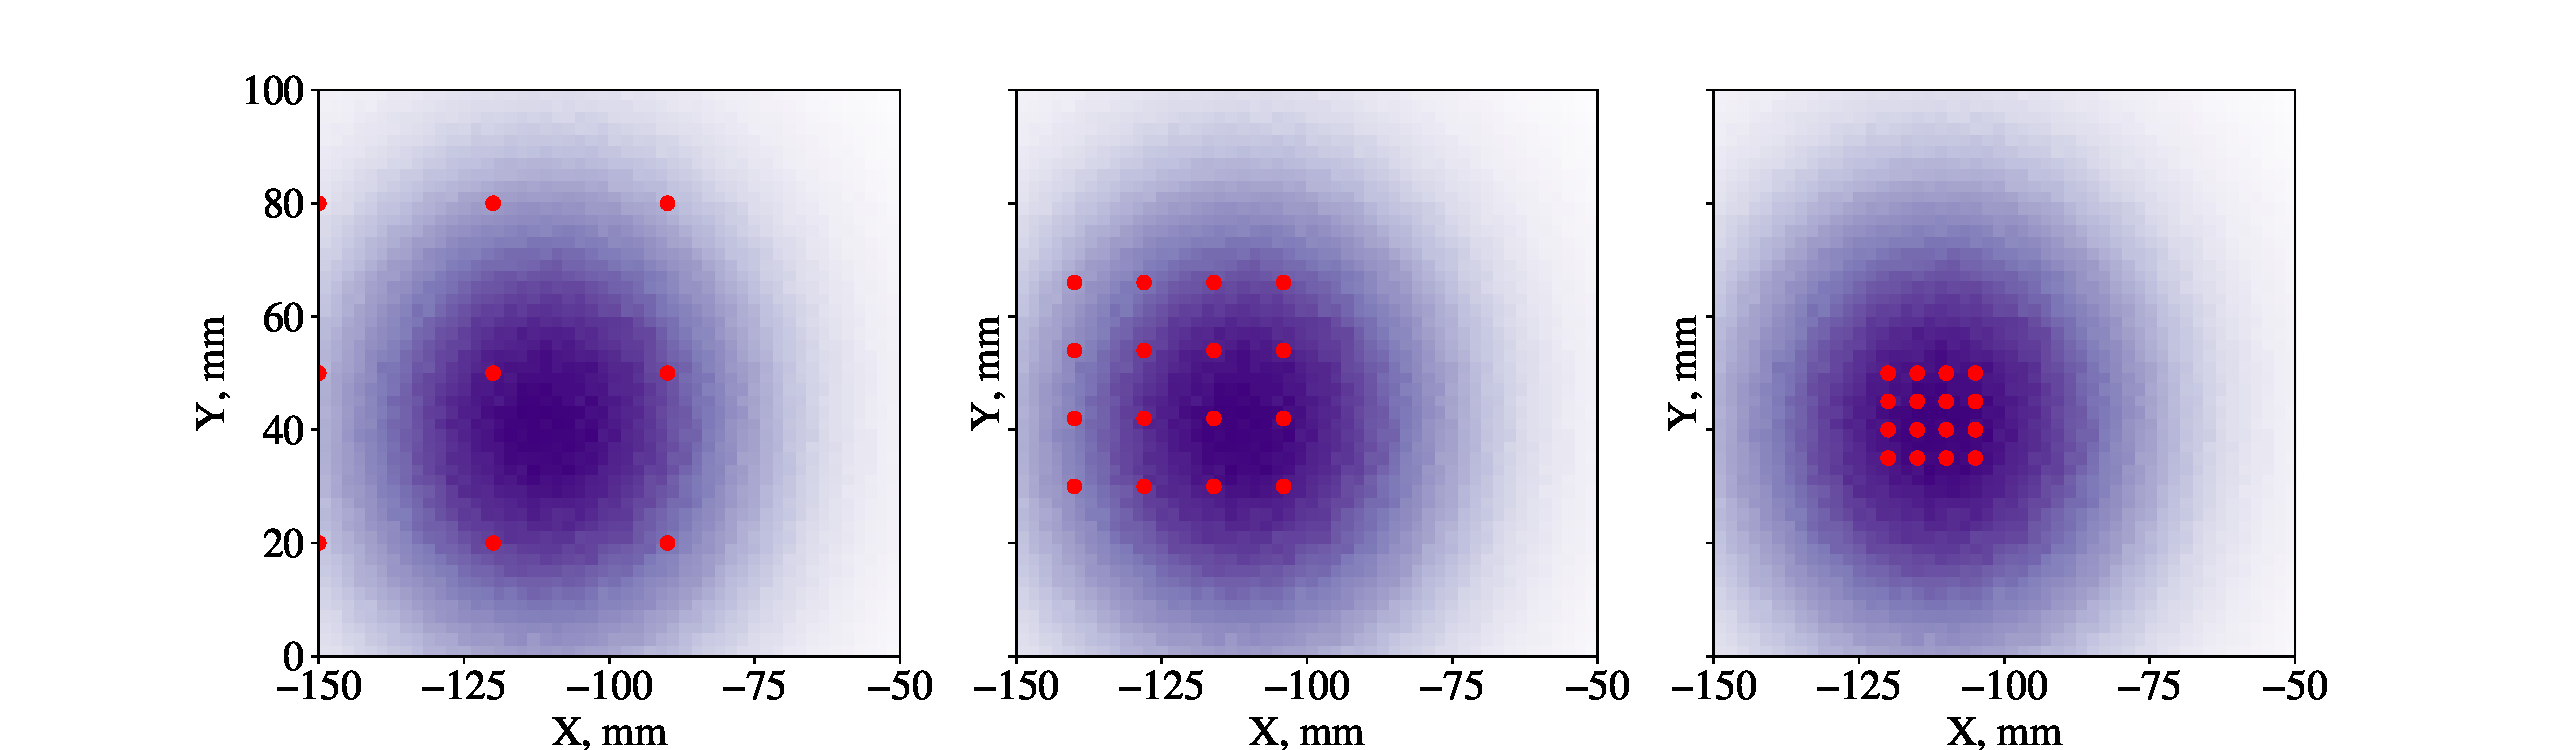
\includegraphics[width=1\linewidth]{images/grids.pdf}}
	\caption{Визуализация метода сжимающихся сеток}
	\label{ris:grids}
\end{figure}
На каждой итерации при минимизации производится восстановление энергии. Энергия определялась как отношение суммы сигналов со всех ФЭУ и суммы значений LRF в точке с восстановленными координатами.
\\
\par\textbf{Использование калибровочных данных для восстановления формы LRF}
\par
Как уже упоминалось, гамма-кванты, излучаемые использованными калибровочными источниками, имеют большую энергию, достаточную для засвечивания всей верхней матрицы детектора. Это позволяет определять LRF по калибровочным данным и использовать их в дальнейшем при обработке,  в том числе для событий с существенно меньшей энергией. Построение LRF производилось итеративно в соответствии с методикой из~\cite{6154607}  описанным далее способом (схема алгоритма приведена на рисунке~\ref{ris:lrfscheme}). 
\begin{figure}[hbt]
	\center{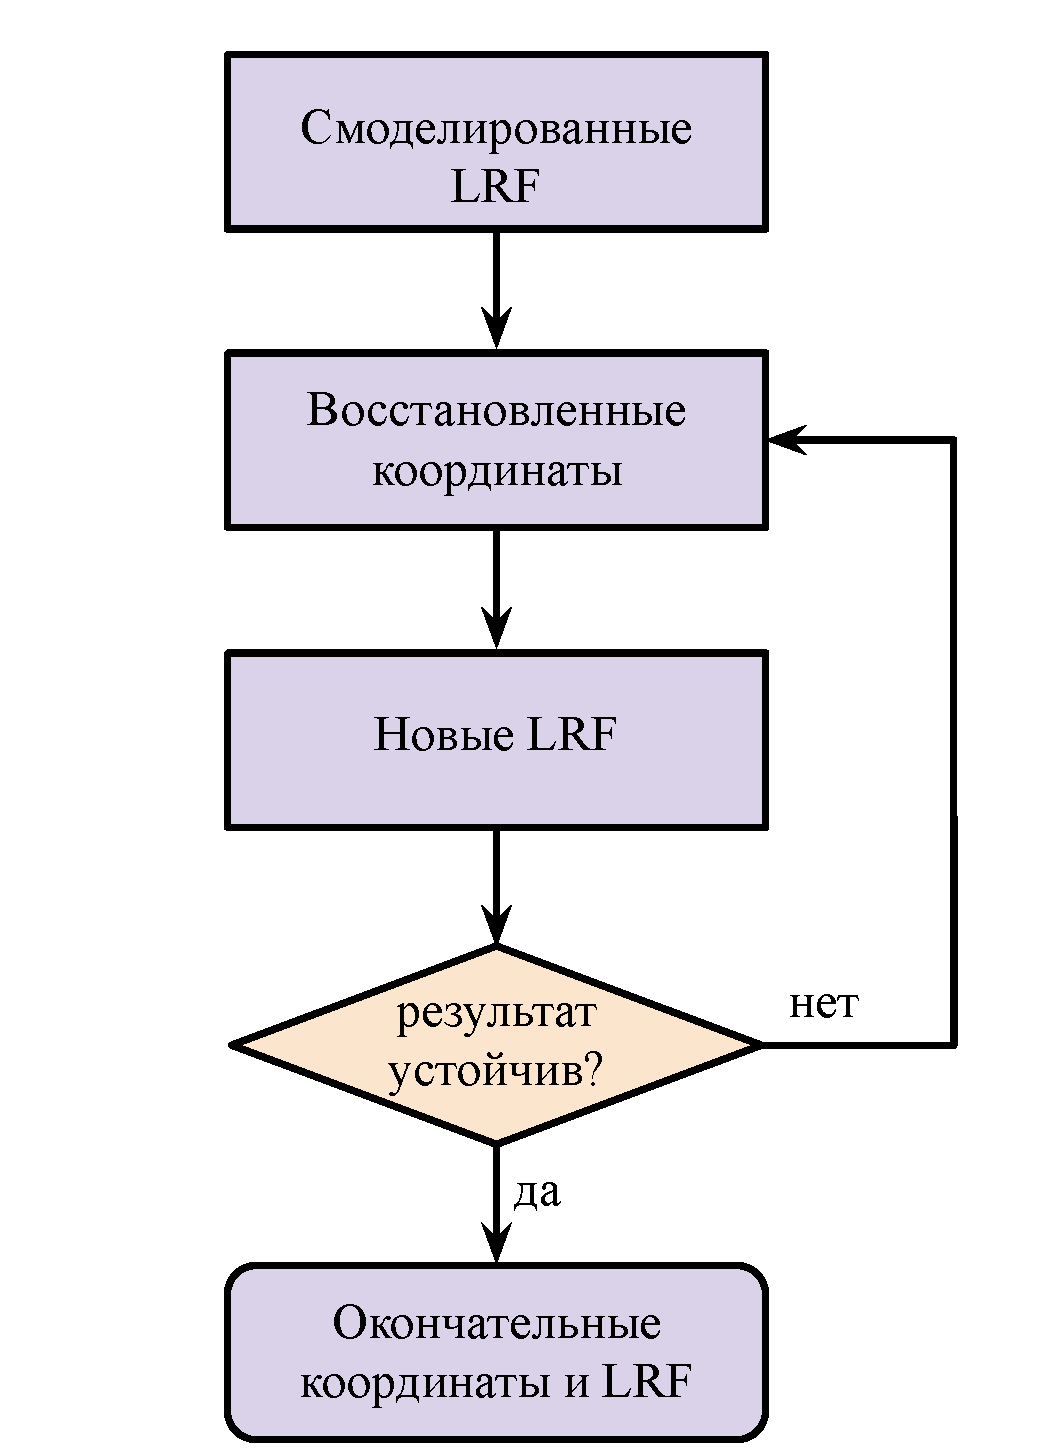
\includegraphics[width=0.6\linewidth]{scheme.pdf}}
	\caption{Алгоритм восстановления координат и LRF}
	\label{ris:lrfscheme}
\end{figure}
Производилось восстановление событий по имеющимся LRF, при этом в качестве начального приближения использовались LRF, построенные в результате моделирования. На основании полученных положений событий и энергии строились новые LRF, а затем новые положения. В качестве стартовых координат при минимизации были выбраны координаты ФЭУ с максимальным откликом в данном событии. При построении LRF не учитывались события, при восстановлении оказавшиеся за пределами детектора. Кроме того, На LRF накладывались следующие ограничения из физических соображений:
\begin{itemize}
    \item функция должна была монотонно убывать с увеличением r;
    \itemв точке $r = 0$ требовалось равенство нулю первой производной по $r$; 
    \itemфункция должна была быть неотрицательна.
\end{itemize}
\parКроме того, для построения LRF ФЭУ группировались в зависимости от расстояния до центра детектора.
Далее опять производилось восстановление координат. Процесс повторялся итеративно до достижения устойчивого результата, что означает, что последующие итерации не приводят к заметным изменениям в восстановленных координатах.

\subsection{Калибровки гамма-источниками во время инженерного сеанса}
\label{subsect3_3_4}
В рамках физических тестов детектора РЭД-100 в ЛЭЯФ НИЯУ МИФИ в 2019 году были набраны данные с использованием калибровочных радиоактивных источников $^{60}$Co и $^{22}$Na. В процессе распада данные элементы излучают гамма-кванты с энергиями 511 кэВ ($^{22}$Na), 1173 кэВ и 1333 кэВ ($^{60}$Co). При наборе данных источники находились на определеной высоте с одной стороны детектора, источник $^{60}$Co был коллимирован, а для набора данных с источником $^{22}$Na была задействована схема совпадений с детектором NaI[Tl] После процедур поиска импульсов и кластеризации для получения LRF были использованы события от $^{60}$Co, на которые были наложены отборы, позволившие отобрать события из пика.
\begin{figure}[hbt]
	\center{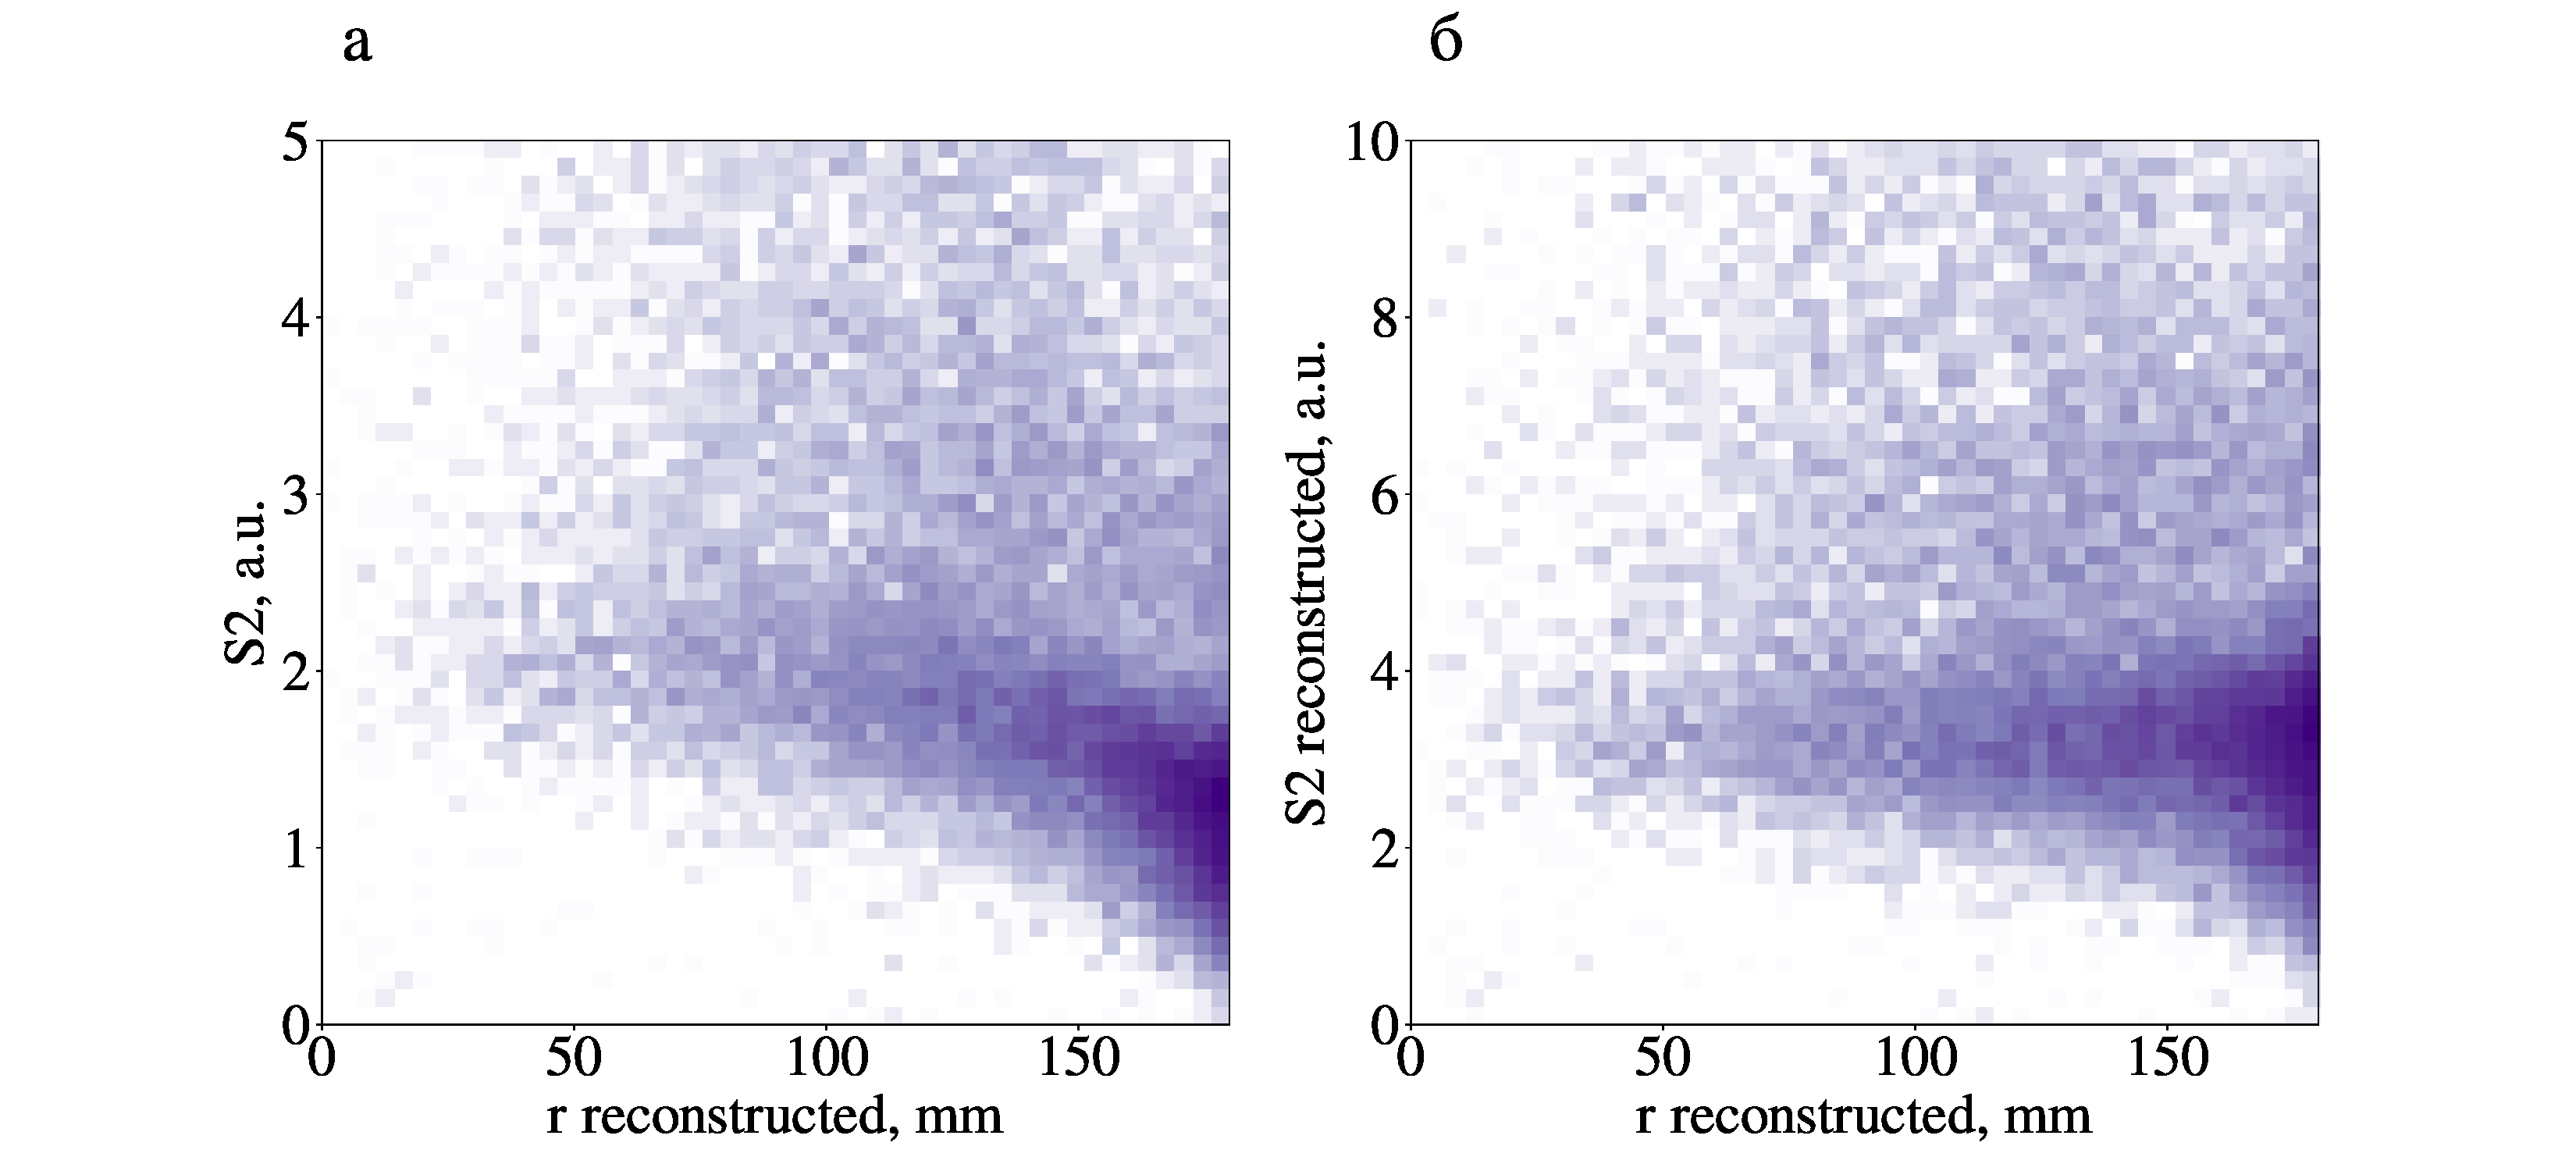
\includegraphics[width=1\linewidth]{energyvsr.pdf}}
	\caption{Зависимость суммарного сигнала(а) и восстановленной энергии S2(б) от восстановленного радиуса}
	\label{img:s2vsR2019}
\end{figure}
\parНа рисунке \ref{img:s2vsR2019}(a) представлена зависимость суммарного (не скорректированного) сигнала от восстановленного радиуса. События ближе к краю детектора дают меньший отклик, чем события в центре за счет краевых эффектов. Энергия, восстановленная при помощи описанного выше алгоритма, не падает с увеличением расстояния от центра детектора (рисунок \ref{img:s2vsR2019}(б)), что косвенно указывает корректность проведенной процедуры восстановления. 

С использование полученных LRF было произведено восстановление координат и энергии для событий от $^{22}$Na. Пространственное распределение событий от источников представлено на рисунке~\ref{img:xyplot2019}.
Распределение событий по S1 и S2 до и после коррекции представлено на рисункax~\ref{img:s1s2na},~\ref{img:s1s2co}. Видно, что после коррекции на распределении для $^{60}$Co становятся различимы линии 1173 кэВ и 1333 кэВ, а для $^{22}$Na --- линия 511 кэВ становится более четкой. Для увеличения соотношения сигнал/шум при построении энергетического спектра на события накладывались ограничения на глубину исходя из известного положения источника, восстановленный полярный угол ($\pi/4$, направленный на источник) и расстояние от центра детектора (<175~мм). На рисунках~\ref{img:s1s2co},~\ref{img:s1s2na} видно, как улучшается разрешение для пика от $^{22}$Na и разрешаются пики от $^{60}$Co после восстановления энергии. Экспериментальный энергетический спектр фитировался одним распределением Гаусса в случае $^{22}$Na и суммой двух распределений Гаусса в случае $^{60}$Co.

Полученный калибровочный график и зависимость энергетического разрешения от энергии представлены на рисунке~\ref{img:calibplot2019}. Линейность калибровочного графика свидетельствует о правильности работы детектора и произведенной обработки данных. Значения положений пиков и энергетического разрешения (отношения среднеквадратичного отклонения ($\sigma$) и ширины на полувысоте (FWHM) к положению пиков) также приведены в таблице~\ref{tab:resolution2019}. 

\begin{figure}[H]
	\center{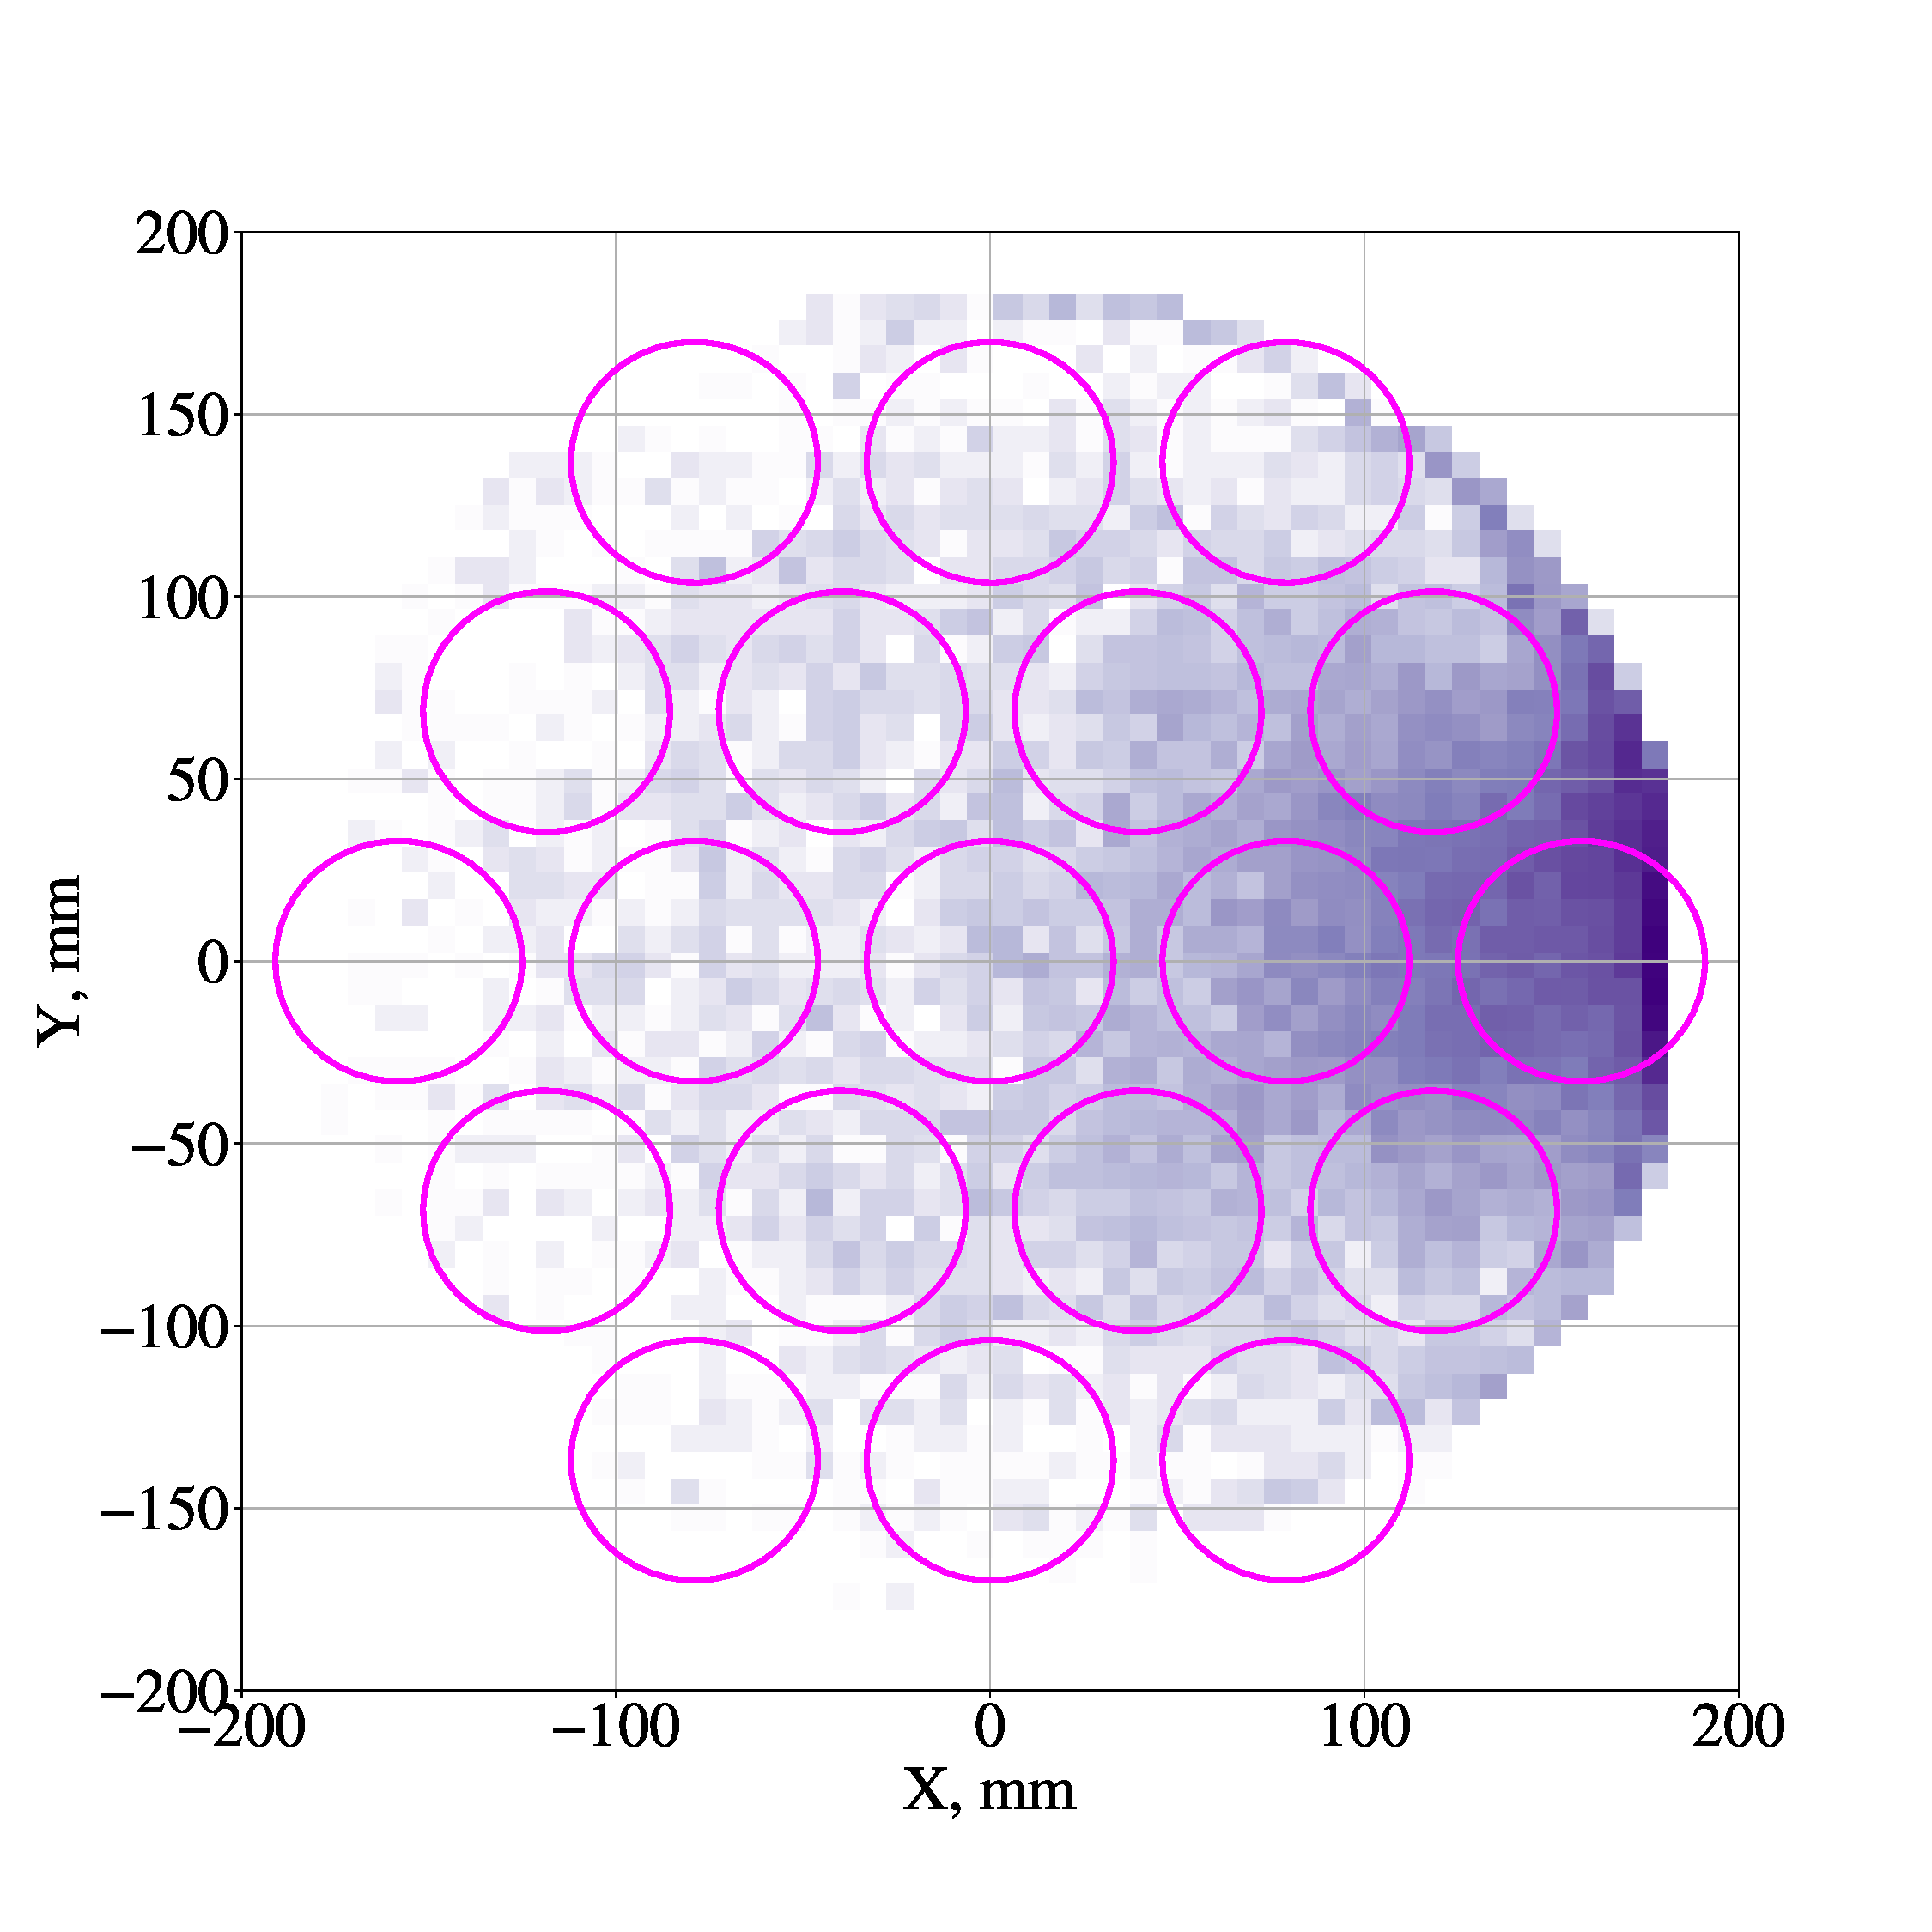
\includegraphics[width=0.6\linewidth]{images/NaXY.pdf}}
	\caption{Распределение по плоскости событий от $^{22}$Na во время инженерного сеанса}
	\label{img:xyplot2019}
\end{figure}

\begin{figure}[H]
	\center{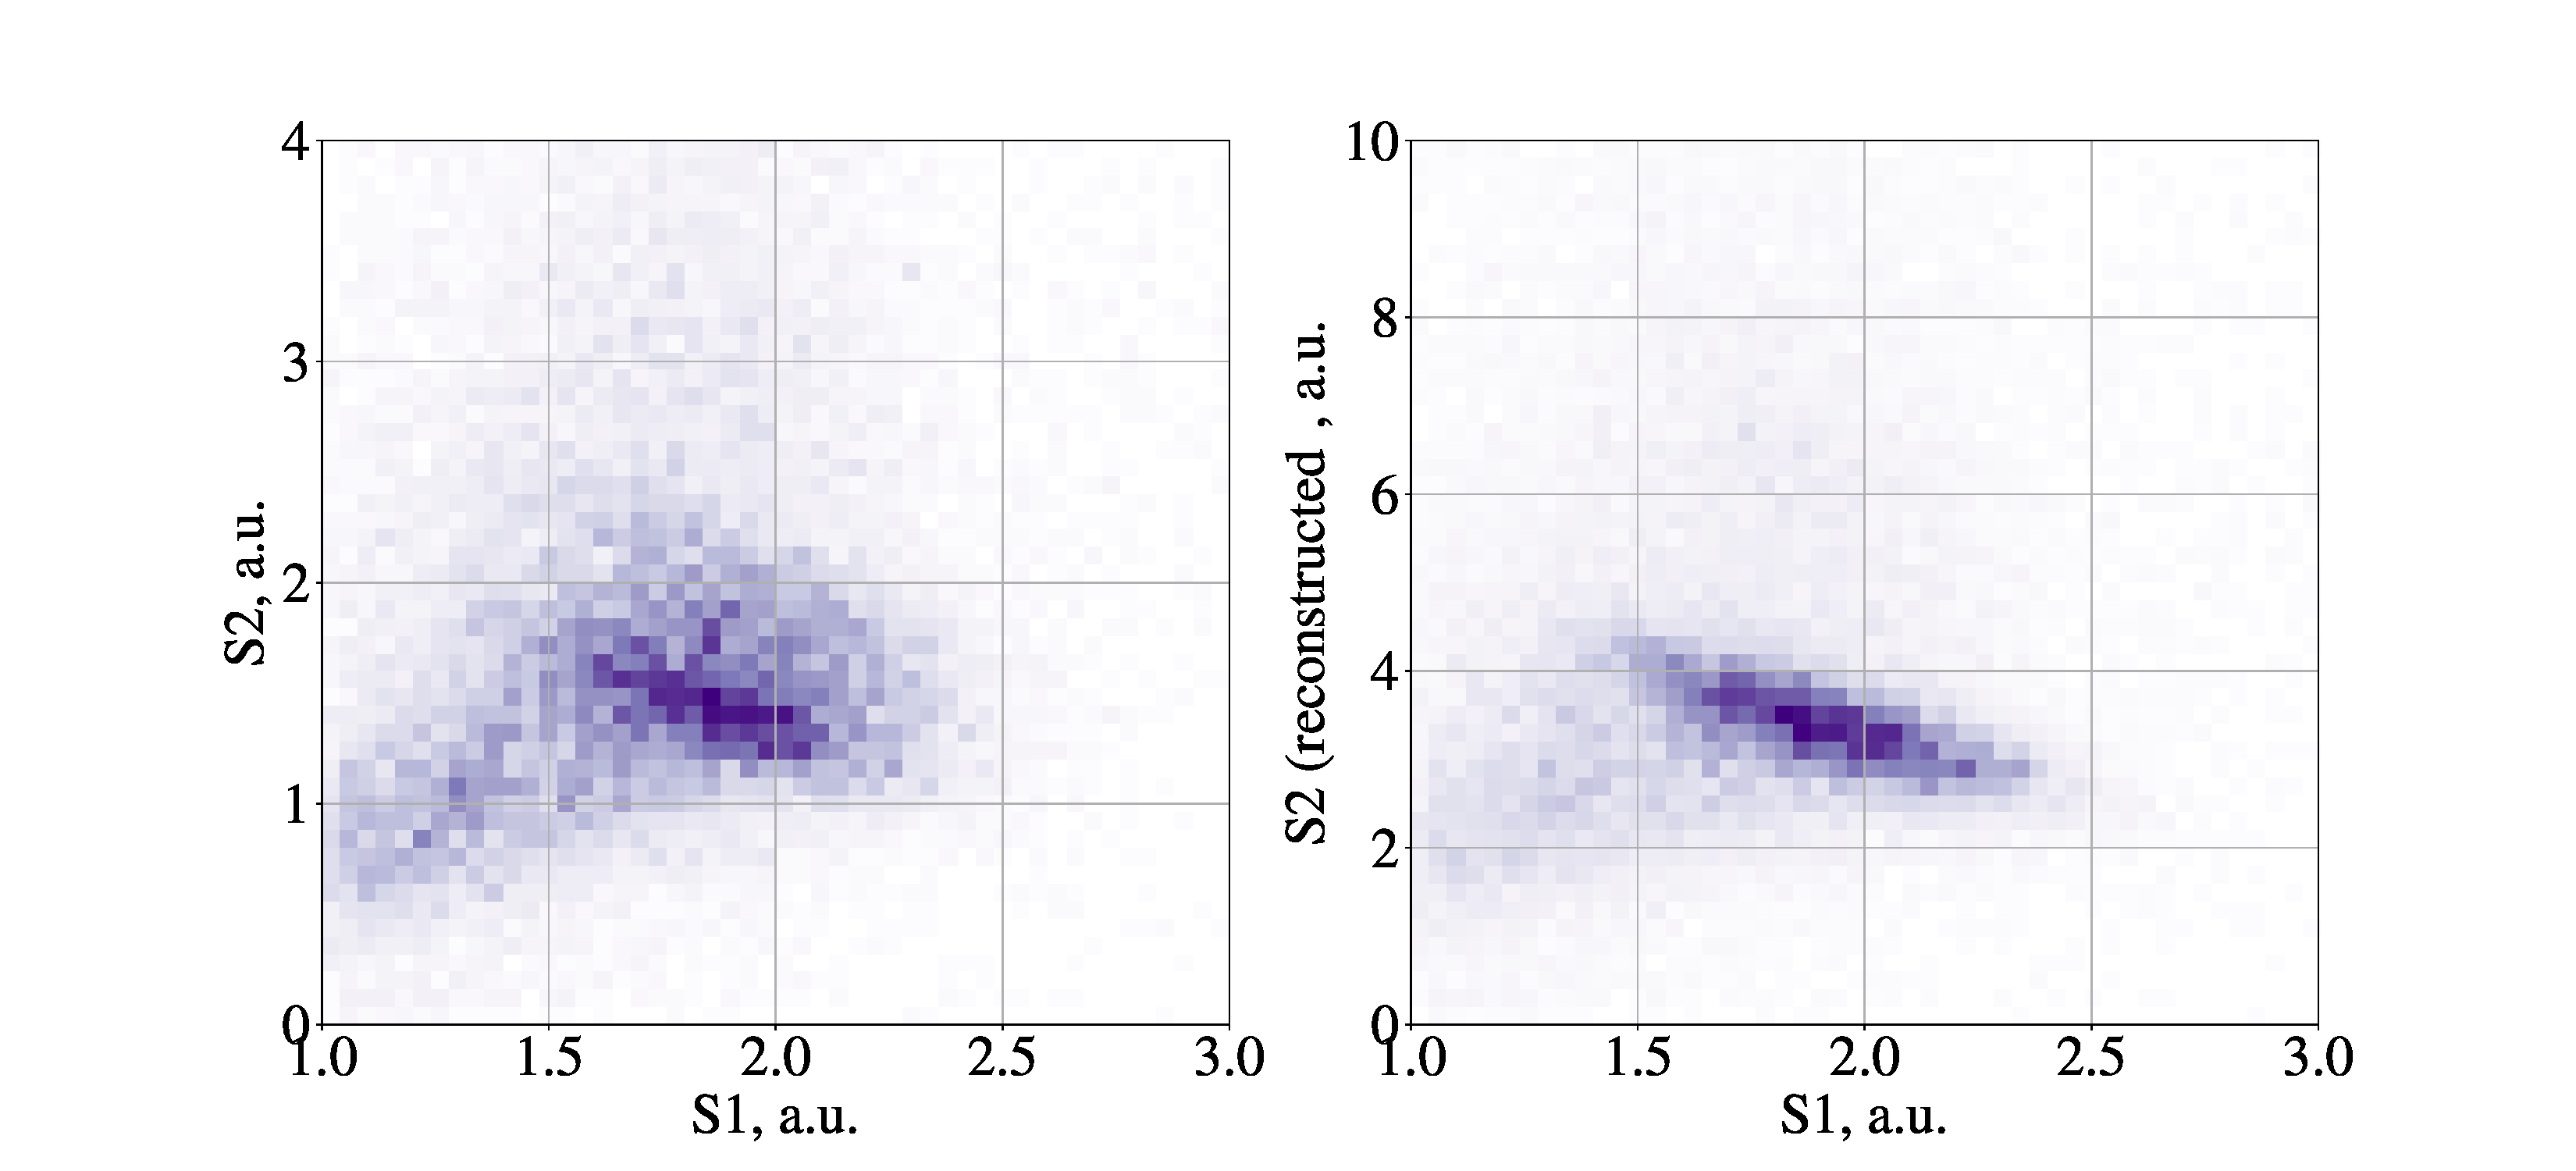
\includegraphics[width=1\linewidth]{images/Nas1s2.pdf}}
	\caption{Распределение событий по S1 и S2 для $^{22}$Na до(слева) и после(справа) восстановления}
  \label{img:s1s2na}  
\end{figure}

\begin{figure}[H]
	\center{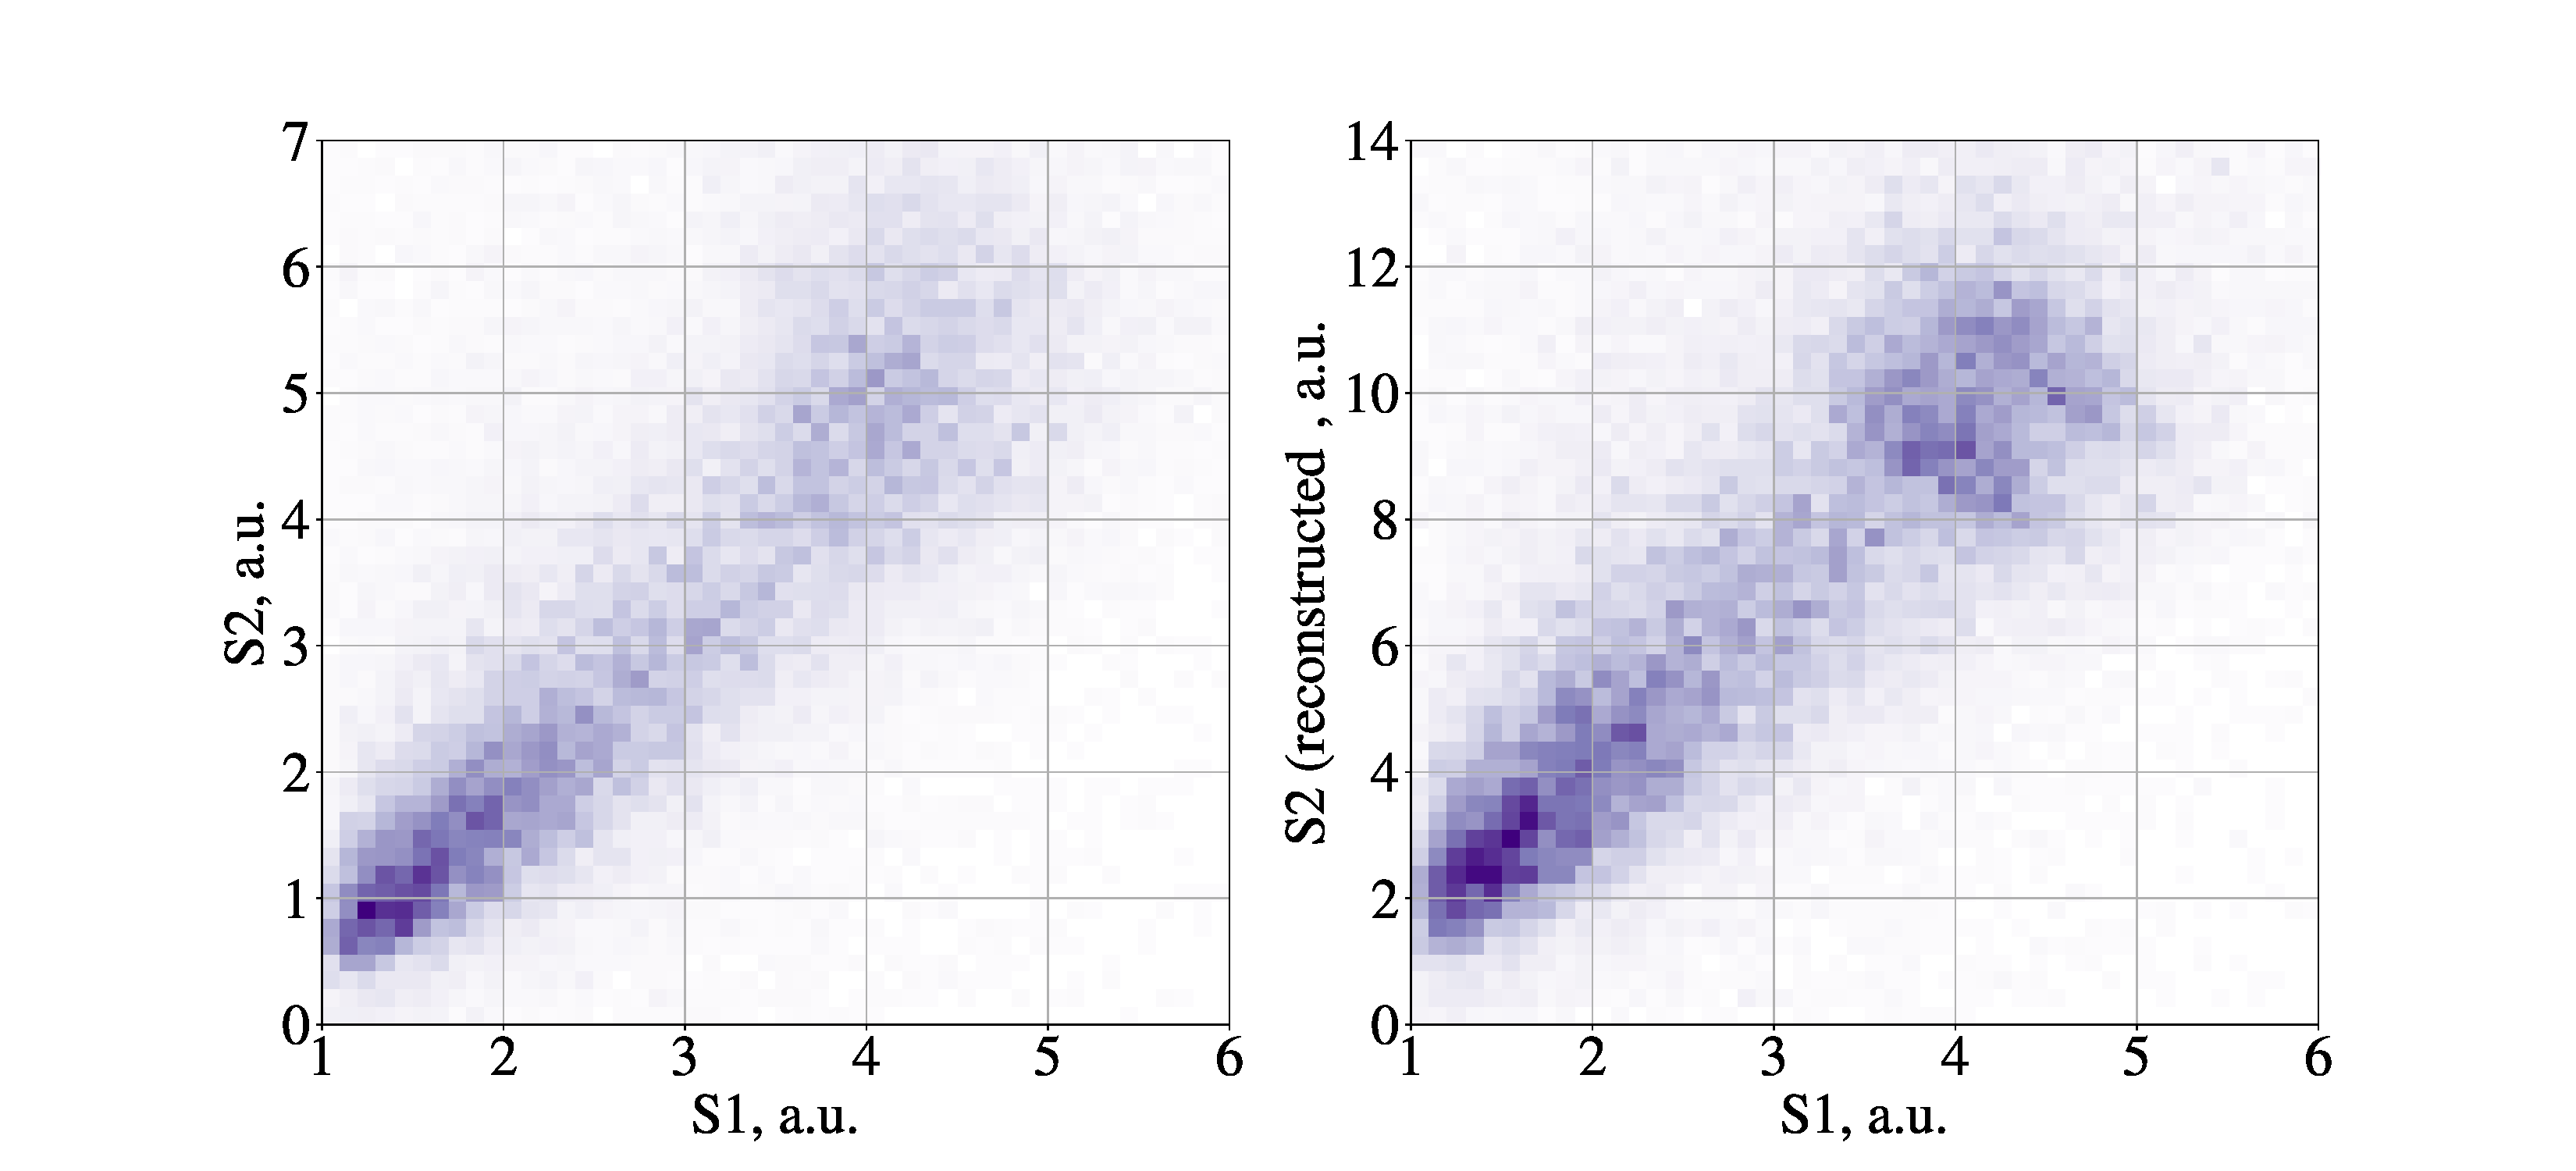
\includegraphics[width=1\linewidth]{images/Cos1s2.pdf}}
	\caption{Распределение событий по S1 и S2 для $^{60}$Co до(слева) и после(справа) восстановления}
  \label{img:s1s2co}  
\end{figure}

\begin{figure}[H]
\center{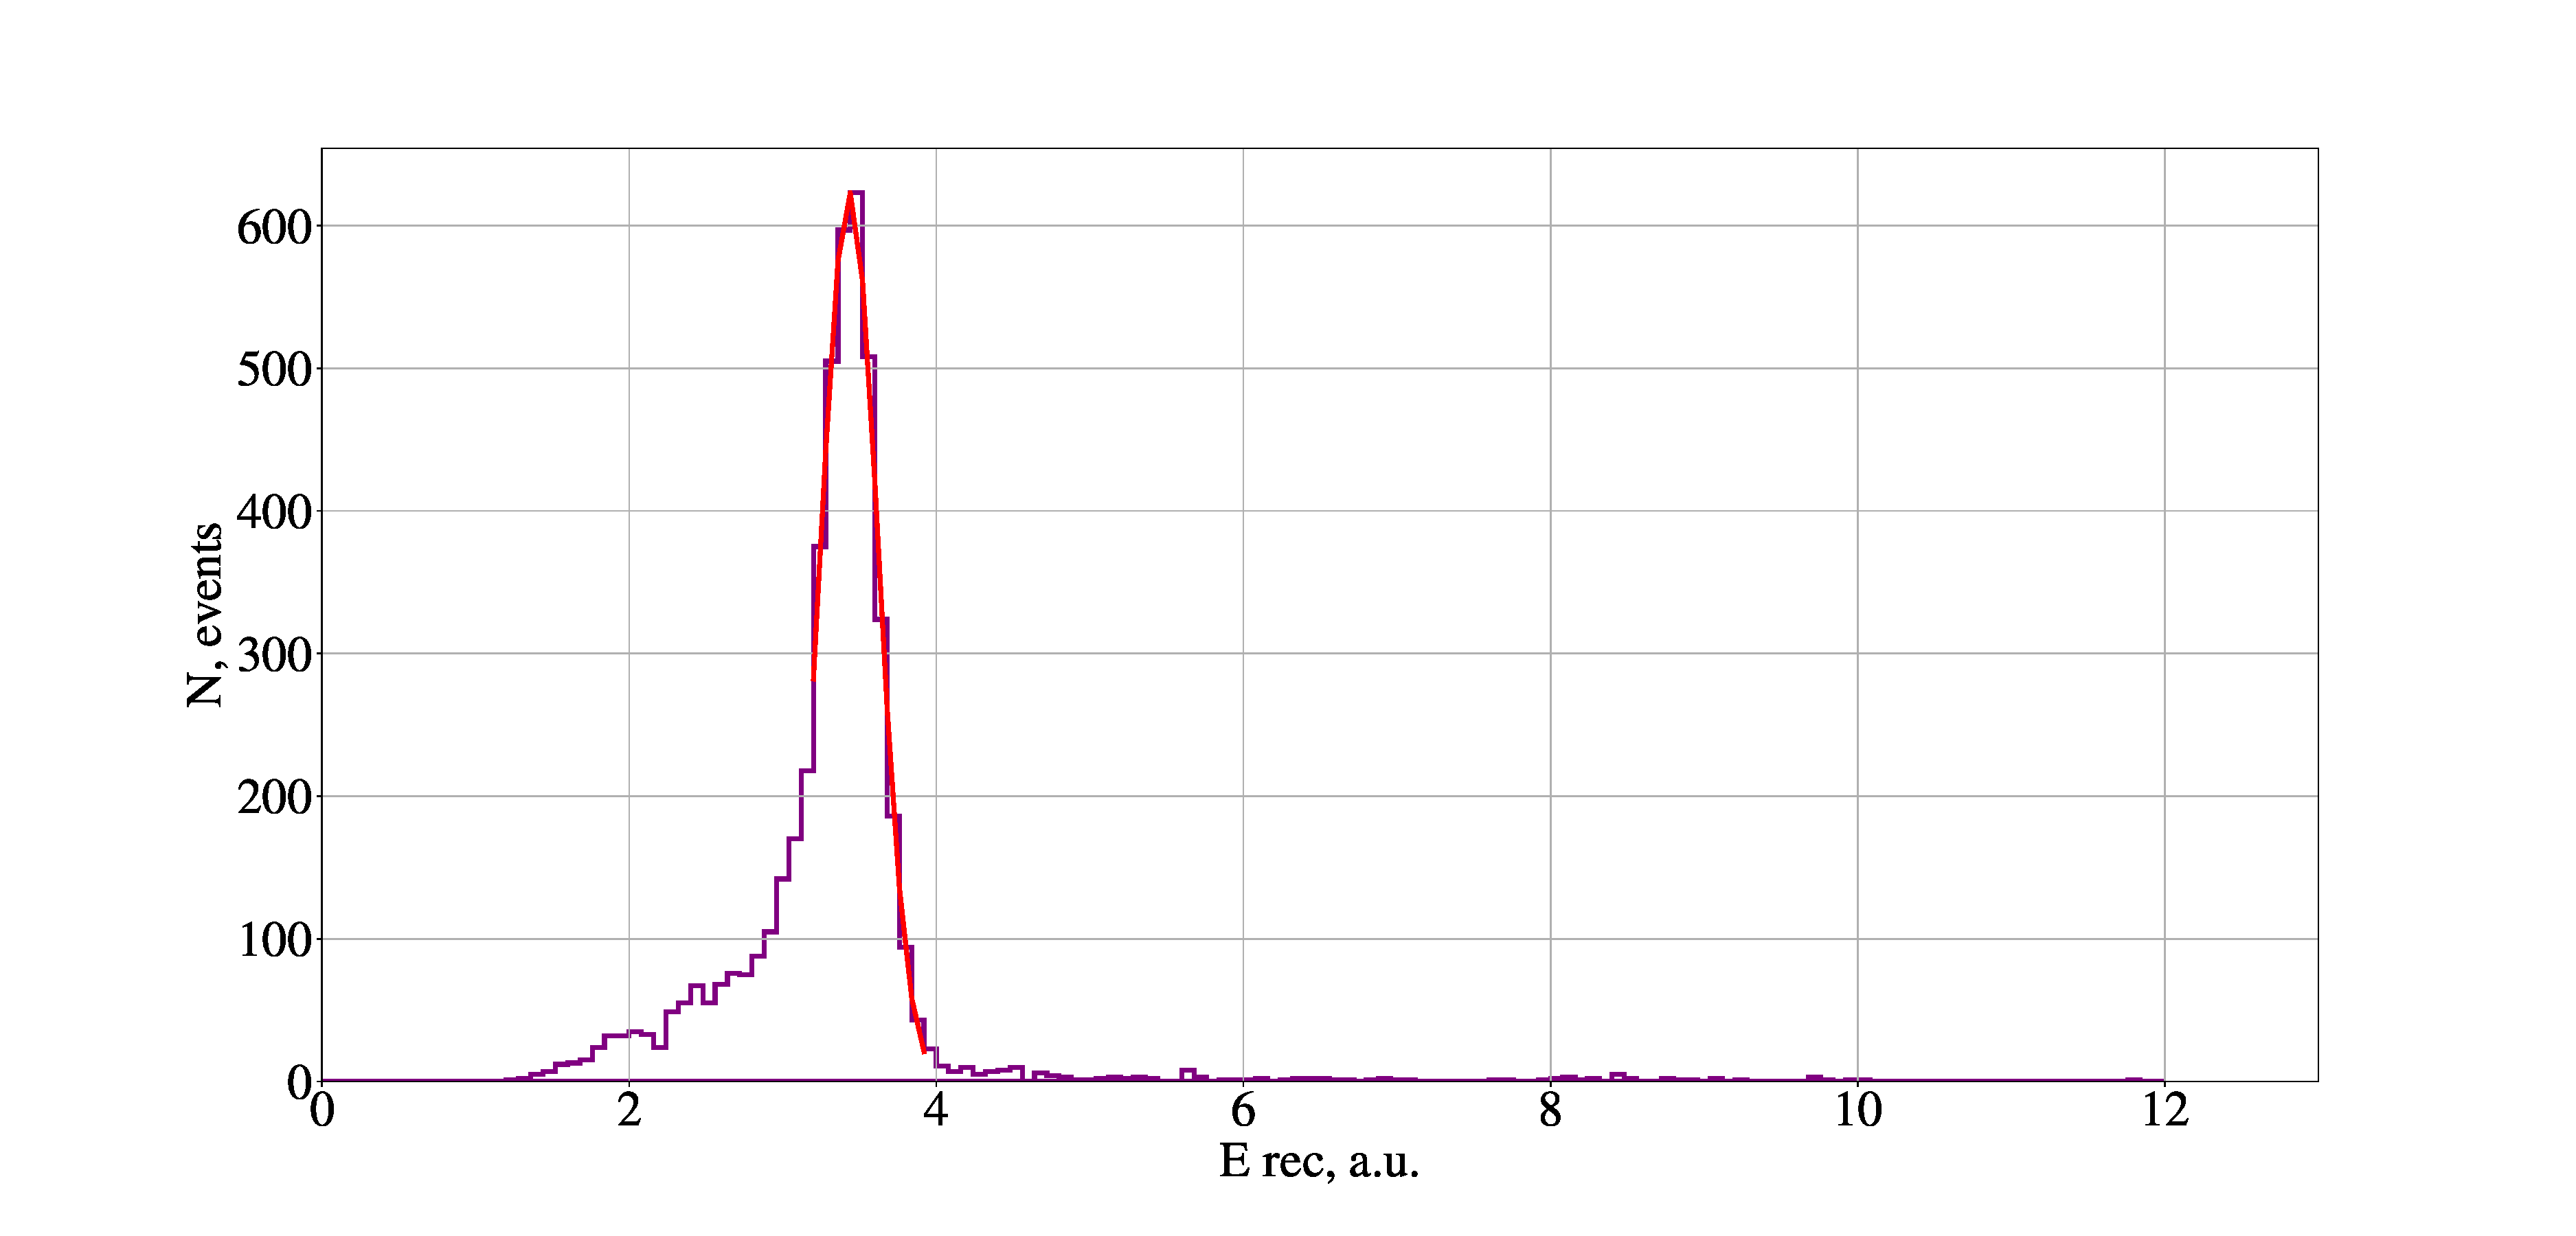
\includegraphics[width=1\linewidth]{images/linecomNa.pdf}}
  \caption{Энергетический спектр от источника $^{22}$Na после восстановления и его фитирование распределением Гаусса}
  \label{img:spectrNa}  
\end{figure}

\begin{figure}[H]
\center{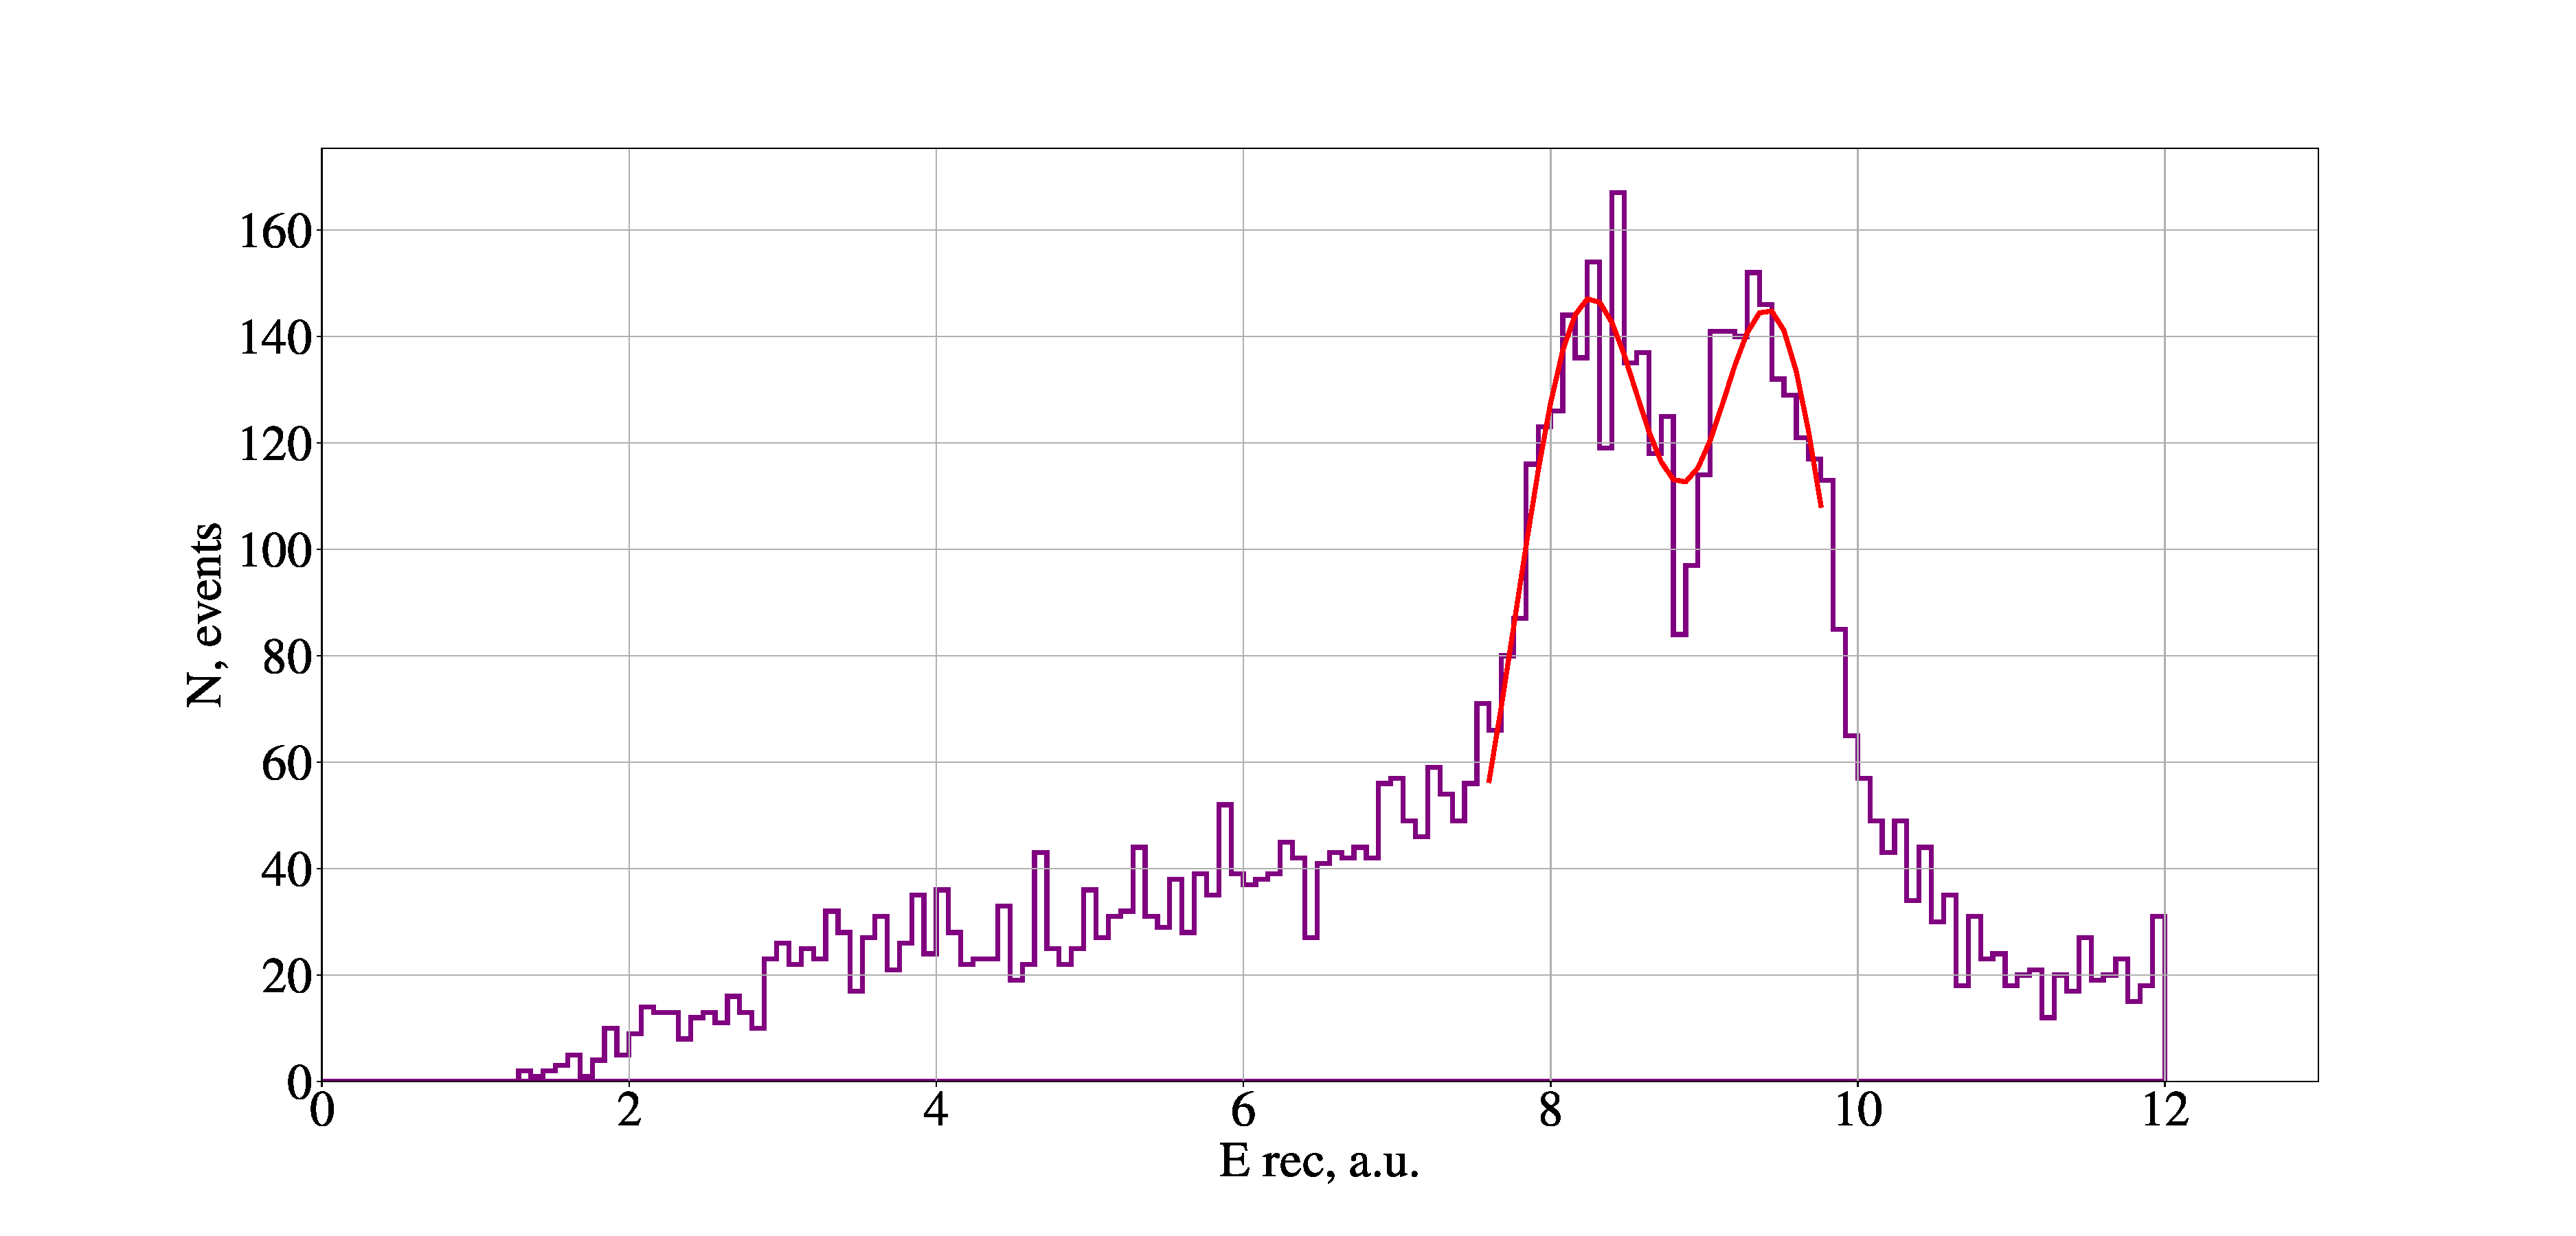
\includegraphics[width=1\linewidth]{images/linecomCo.pdf}}
  \caption{Энергетический спектр от источника $^{60}$Co после восстановления и его фитирование суммой двух распределений Гаусса}
  \label{img:spectrCo}  
\end{figure}

\begin{figure}[H]
\center{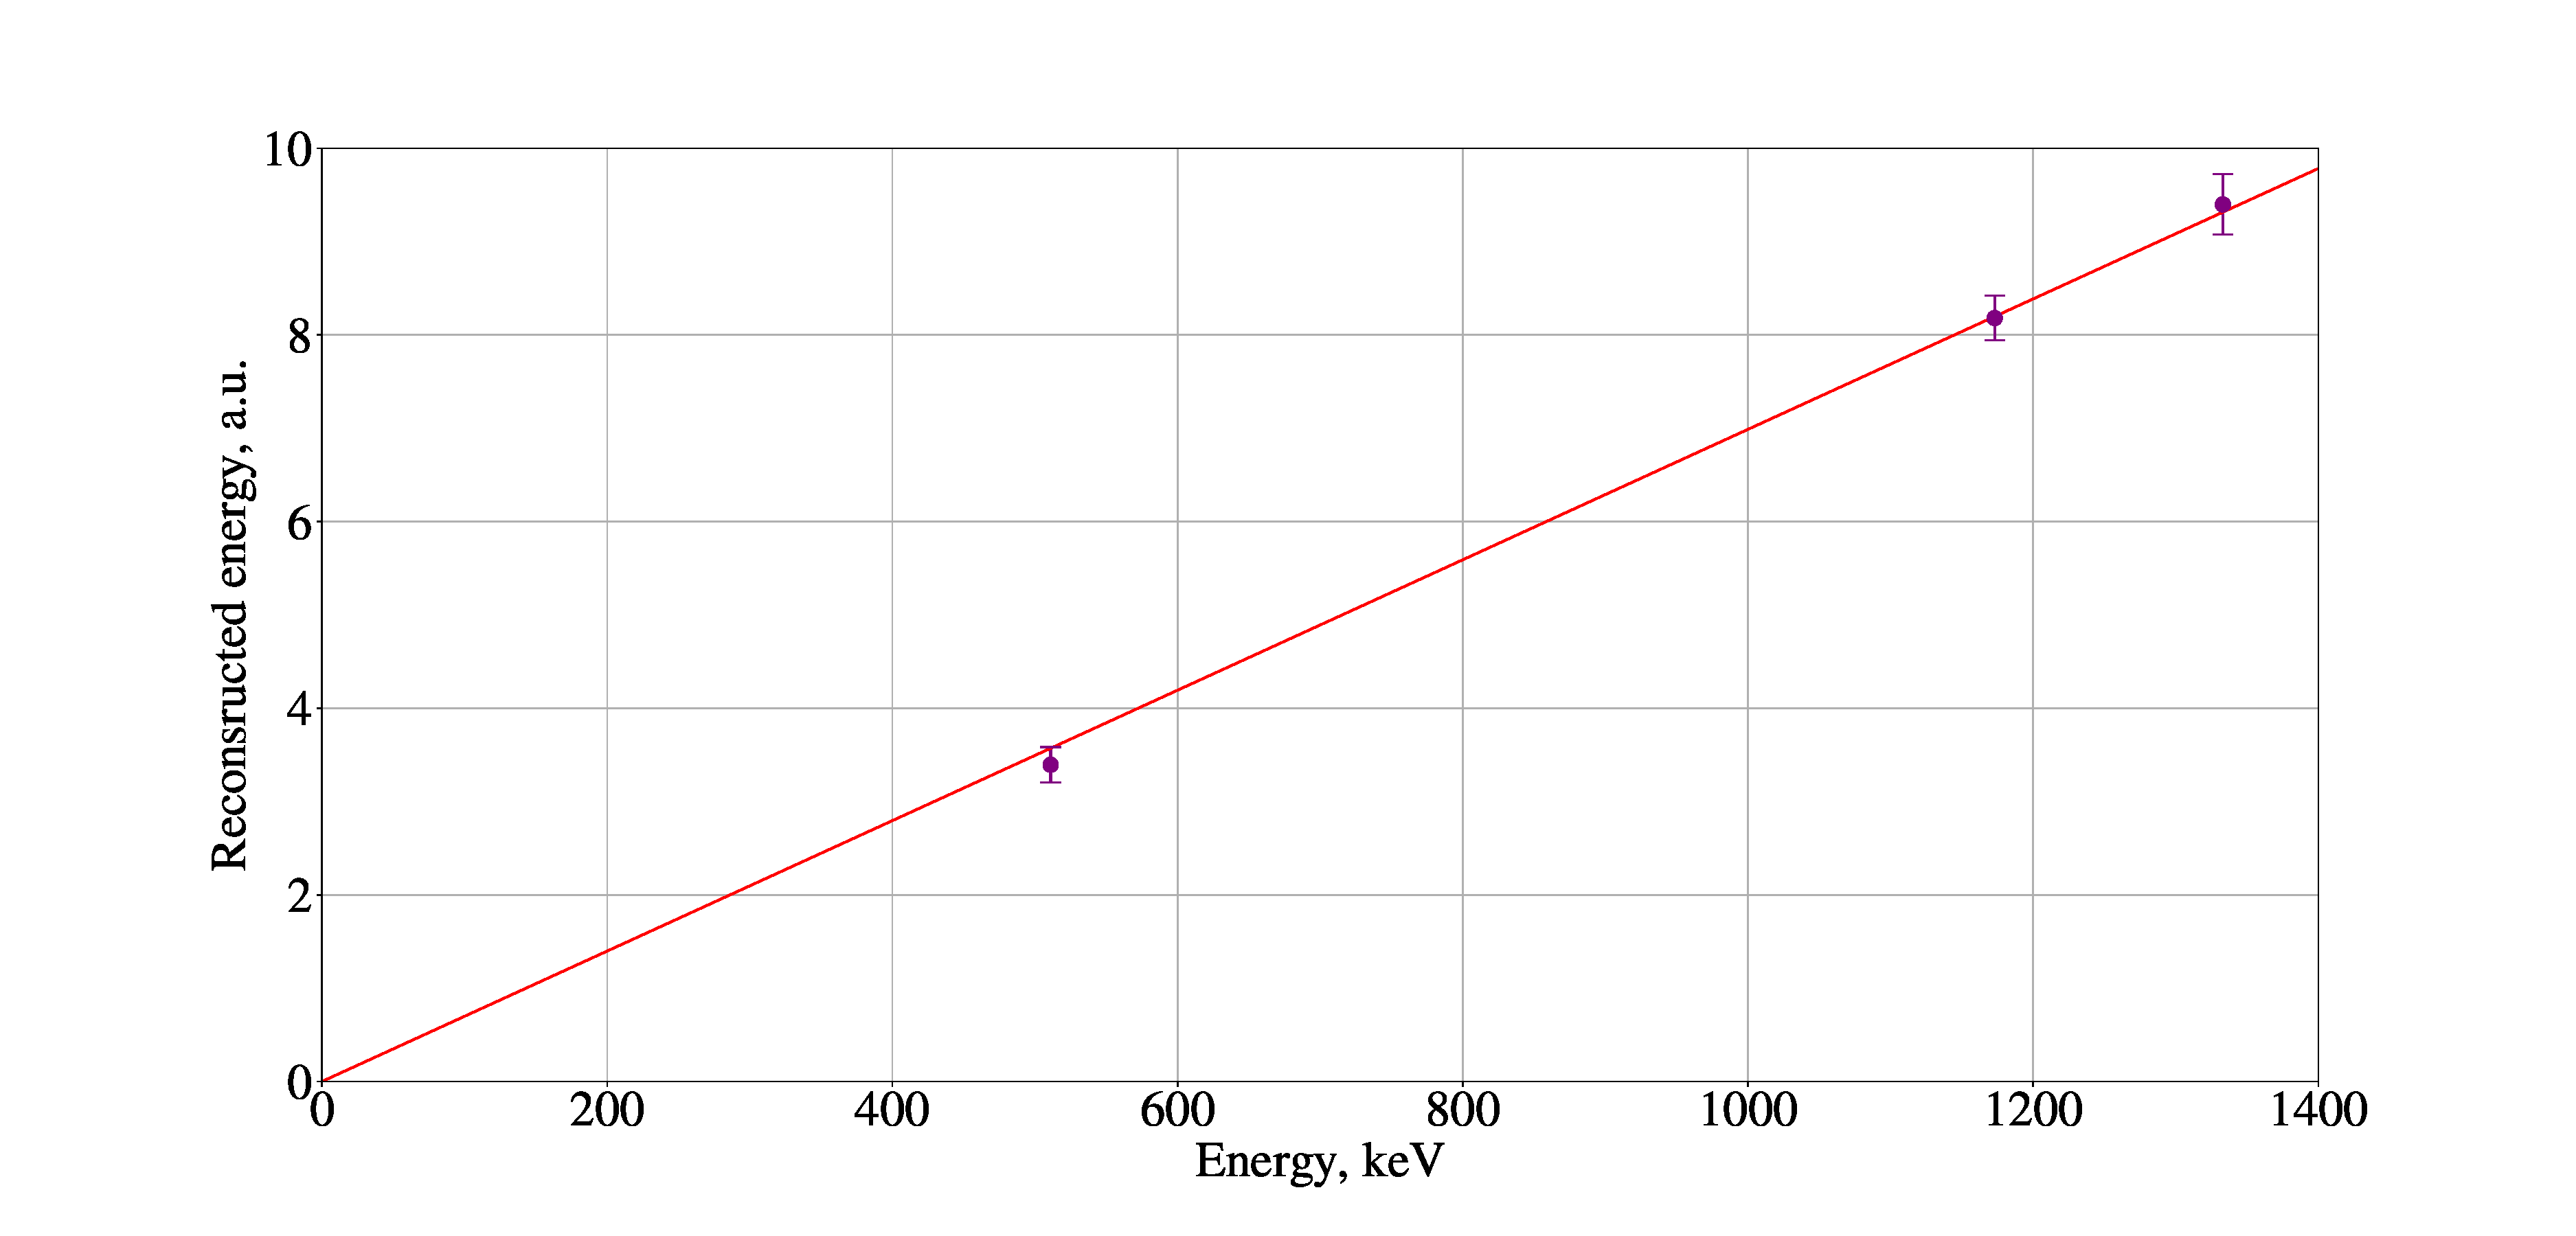
\includegraphics[width=1\linewidth]{images/calibr.pdf}}
  \caption{Калибровочный график для инженерного сеанса 2019 года.}
  \label{img:calibplot2019}  
\end{figure}

\begin{table}[hbt]
    \centering
        \caption{Положения пиков и энергетическое разрешение}
\begin{tabular}{|c|c|c|c|}
\hline
    Энергия, кэВ & Положение пика, кэВ & ($\sigma/E$), \% & FWHM/E,  \%\\
    \hline
    511 & 486$\pm$29 & 5.5$\pm$0.1 & 12.9$\pm$0.2\\
    \hline
    1173 & 1171$\pm$34 & 5.4$\pm$0.1 & 12.7$\pm$0.3\\
    \hline
    1333 & 1345$\pm$46 & 4.8$\pm$0.2 & 11.3$\pm$0.4\\
    \hline
\end{tabular}
    \label{tab:resolution2019}
\end{table}

\subsection{Калибровки гамма-источниками во время сеанса на Калининской АЭС}
\label{subsect3_3_5}

 
\parК сожалению, измерения с гамма-источниками при постановке эксперимента на КАЭС заведомо имели меньшую точность, чем измерения во время инженерного сеанса. Это связано с невозможность коллимирования источников, набора достаточно хорошей статистики и использования схемы совпадений. Кроме того, конструкция установки с учетом пассивной защиты не позволяла расположить источники достаточно близко к криостату детектора.
\parАлгоритмы анализа данных принципиально не отличались, однако были скорректированы параметры отборов. Так, для улучшения соотношения сигнал/фон, отбирались события, находящиеся внутри радиуса 130 мм, аналогичный отбор по радусу в дальнейшем применялся для всех остальных данных, для которых производилось восстановление.
\parНа рисунке~\ref{img:s1s2Co2022} представлены двумерные распределения S1 и S2 до и после восстановления. На рисунке~\ref{img:spectrCo2022} представлен энергетический спектр от источника $^{60}$Co после восстановления и его фитирование суммой двух распределений Гаусса и функции ошибок, описывающей фон. В таблице~\ref{tab:resolution2022} представлены результаты калибровки гамма-источниками, а на рисунке~\ref{img:calibr2022} -- калибровочный график. Видно, что несмотря на худшую статистику энергетическое разрешение для кобальта улучшилось по сравнению с инженерным сеансом. Это связано с существенно более жестким отбором по радиусу (130 мм вместо 175 мм во время инженерного сеанса), а также введением дополнительно функции ошибок для описания фона.
\begin{figure}[H]
\center{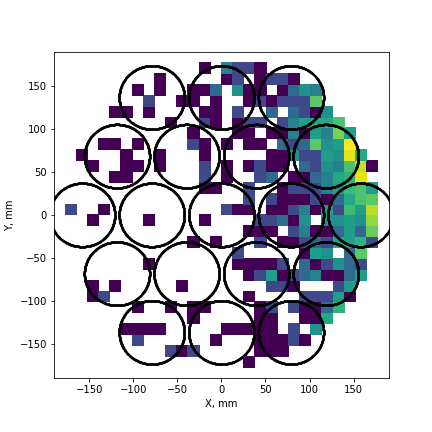
\includegraphics[width=0.5\linewidth]{images/xy_distr.png}}
  \caption{Распределение по плоскости событий от источника $^{60}$Co во время сеанса на КАЭС}
  \label{img:xyCo2022}  
\end{figure}

\begin{figure}[ht]
  \begin{minipage}[ht]{0.49\linewidth}    \center{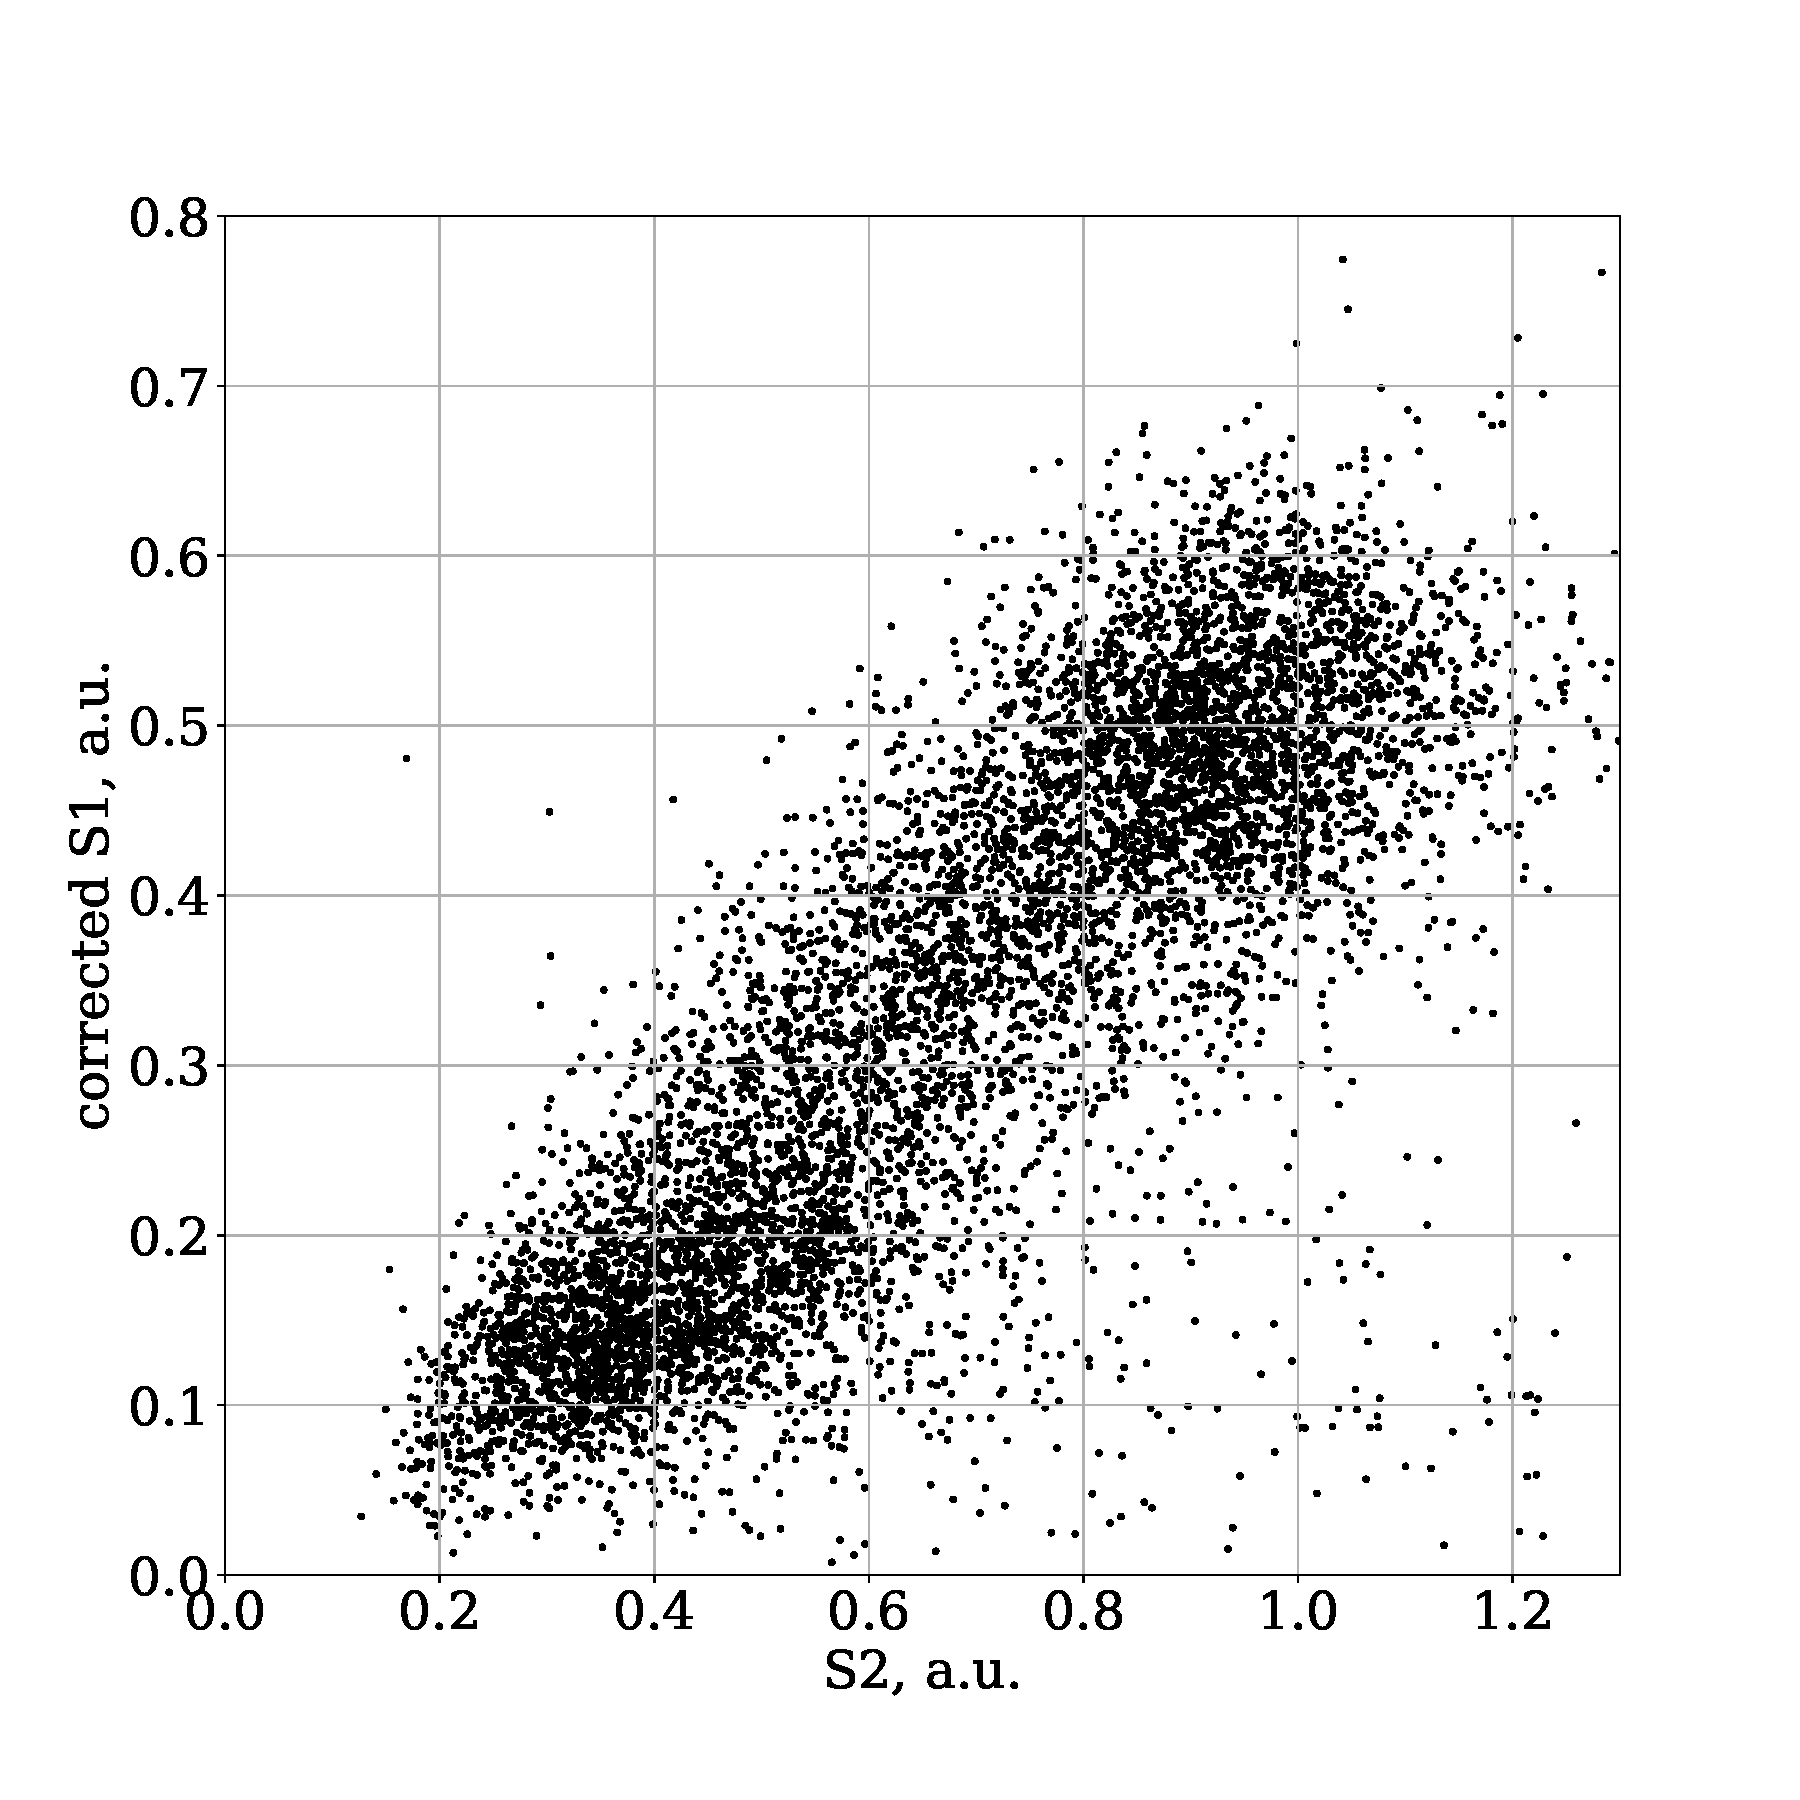
\includegraphics[width=1.0\linewidth]{images/2dspectrum.pdf} \\ а)}
  \end{minipage}
  \hfill
  \begin{minipage}[ht]{0.49\linewidth}  \center{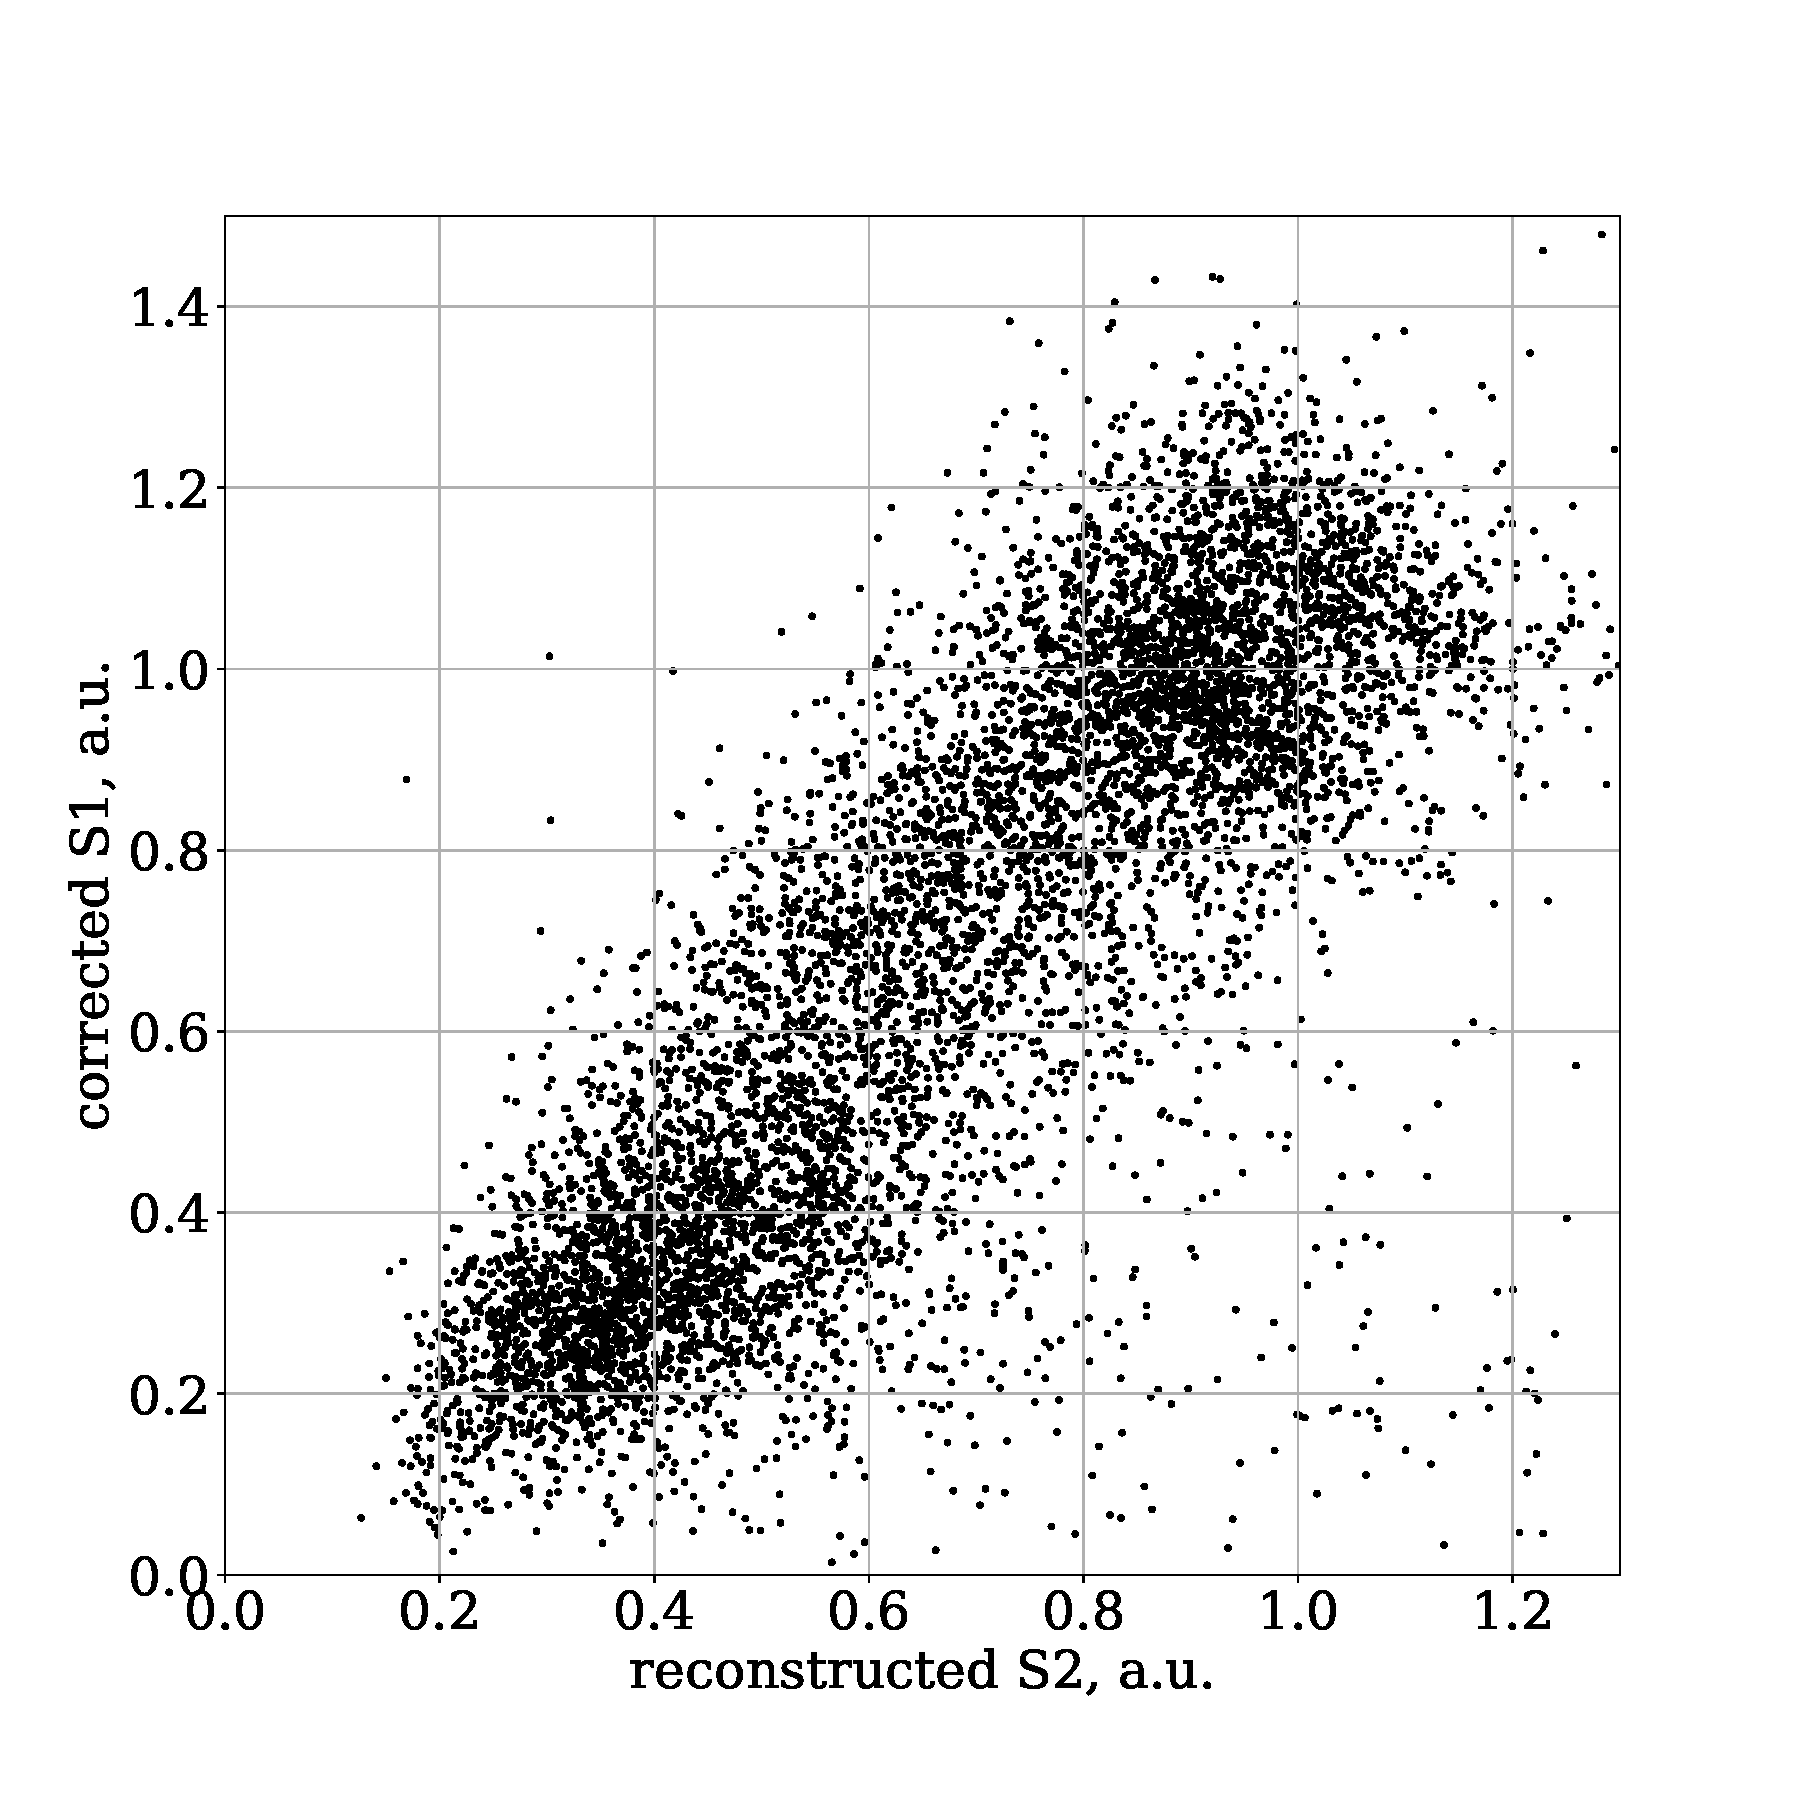
\includegraphics[width=1.0\linewidth]{images/2dspectrum_corr.pdf} \\ б)}
  \end{minipage}
  \caption{Распределение событий по S1 и S2 для $^{60}$Co до(слева) и после(справа) восстановления (сеанс на КАЭС)}
  \label{img:s1s2Co2022}  
\end{figure}

\begin{figure}[H]
\center{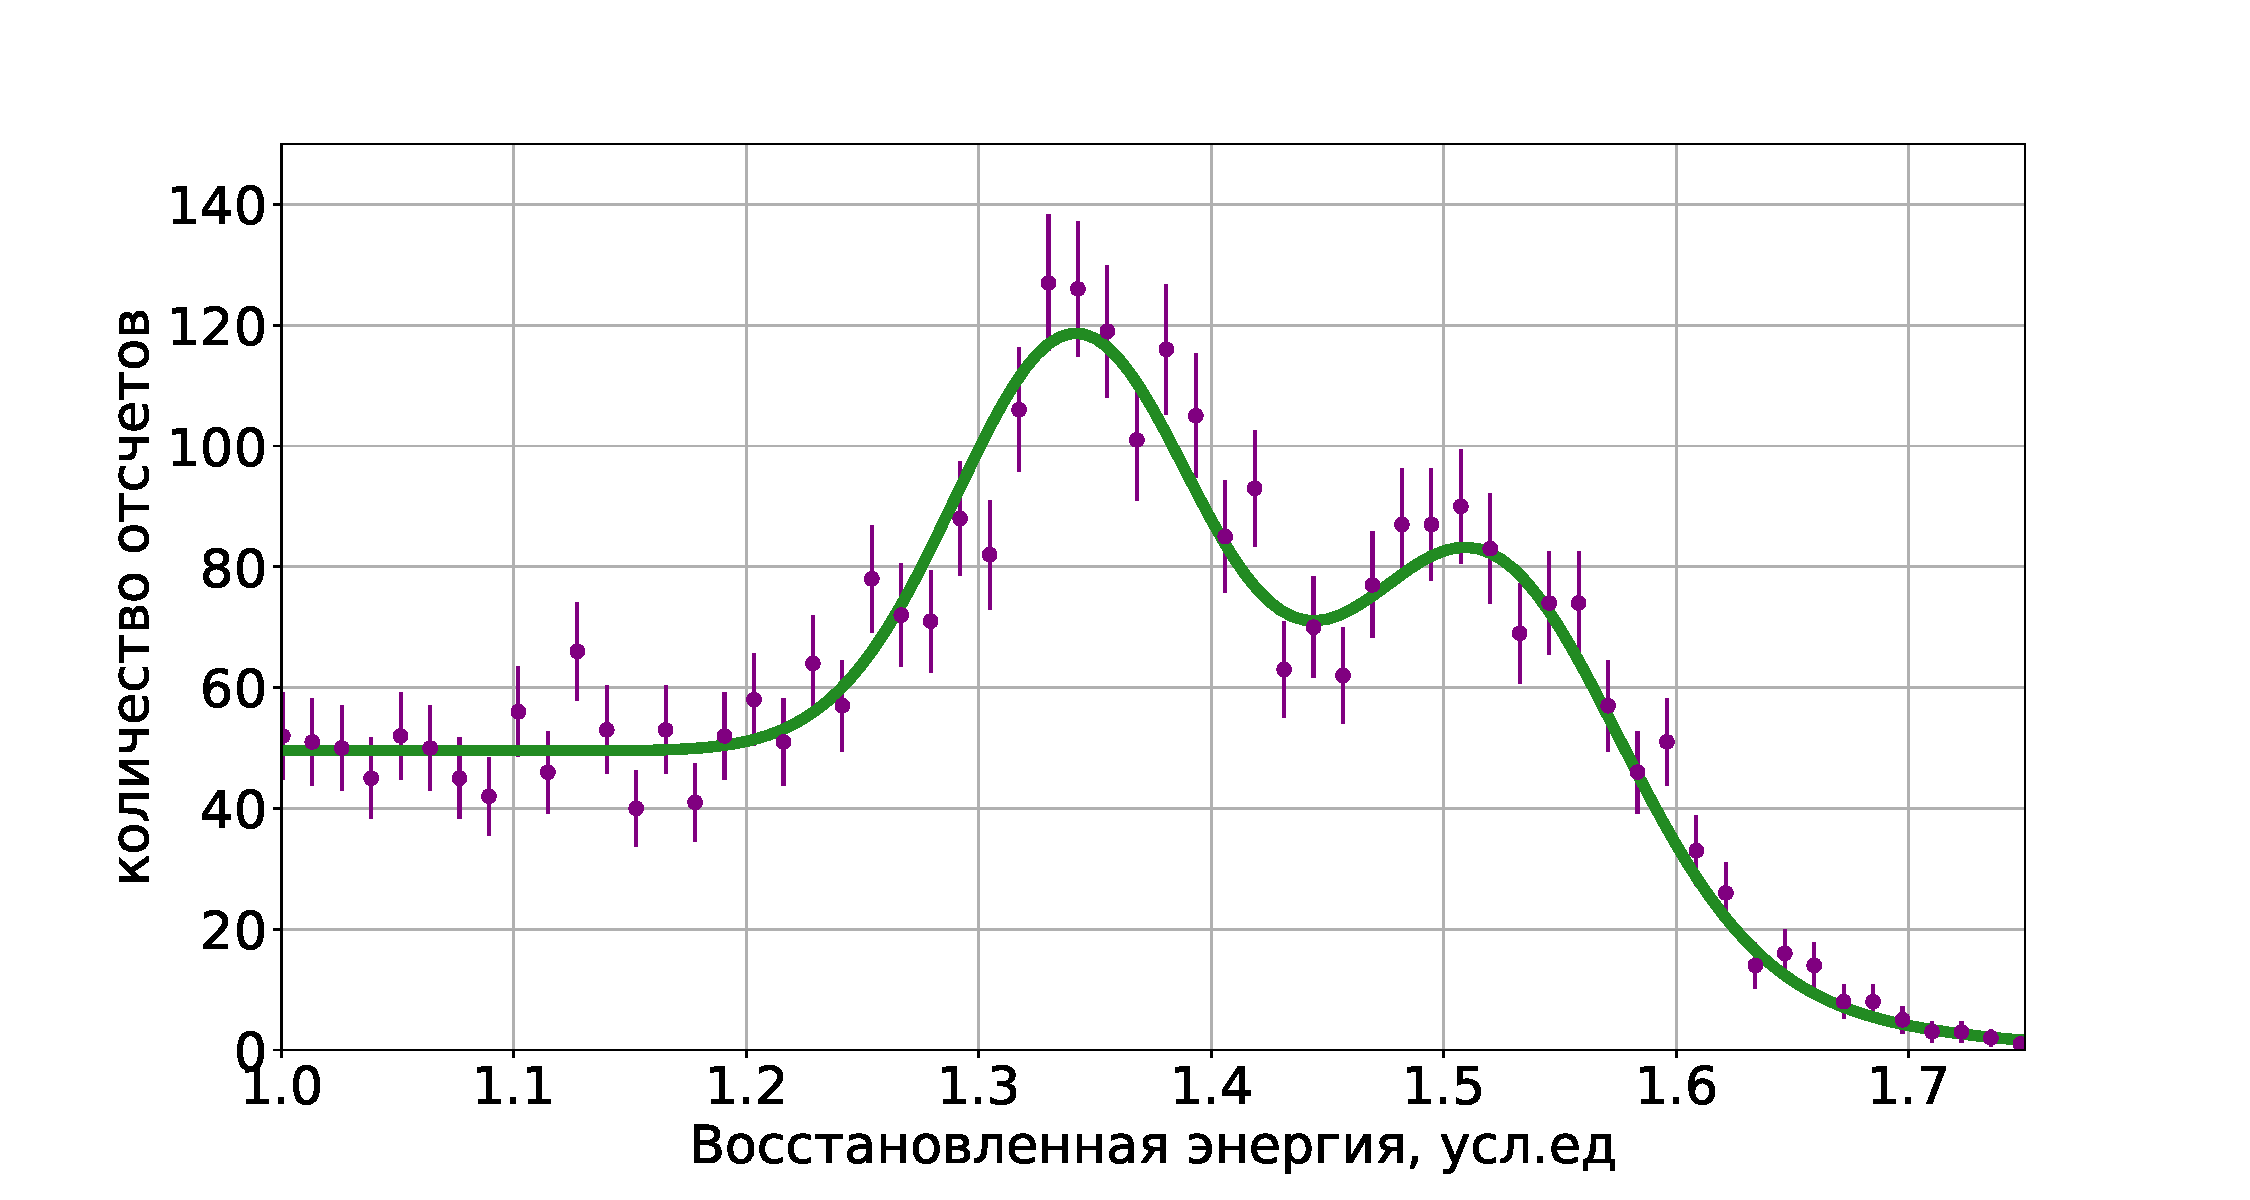
\includegraphics[width=1\linewidth]{images/spectrco2022.pdf}}
  \caption{Энергетический спектр от источника $^{60}$Co после восстановления и его фитирование суммой двух распределений Гаусса и функции ошибок, описывающей фон}
  \label{img:spectrCo2022}  
\end{figure}

\begin{figure}[H]
\center{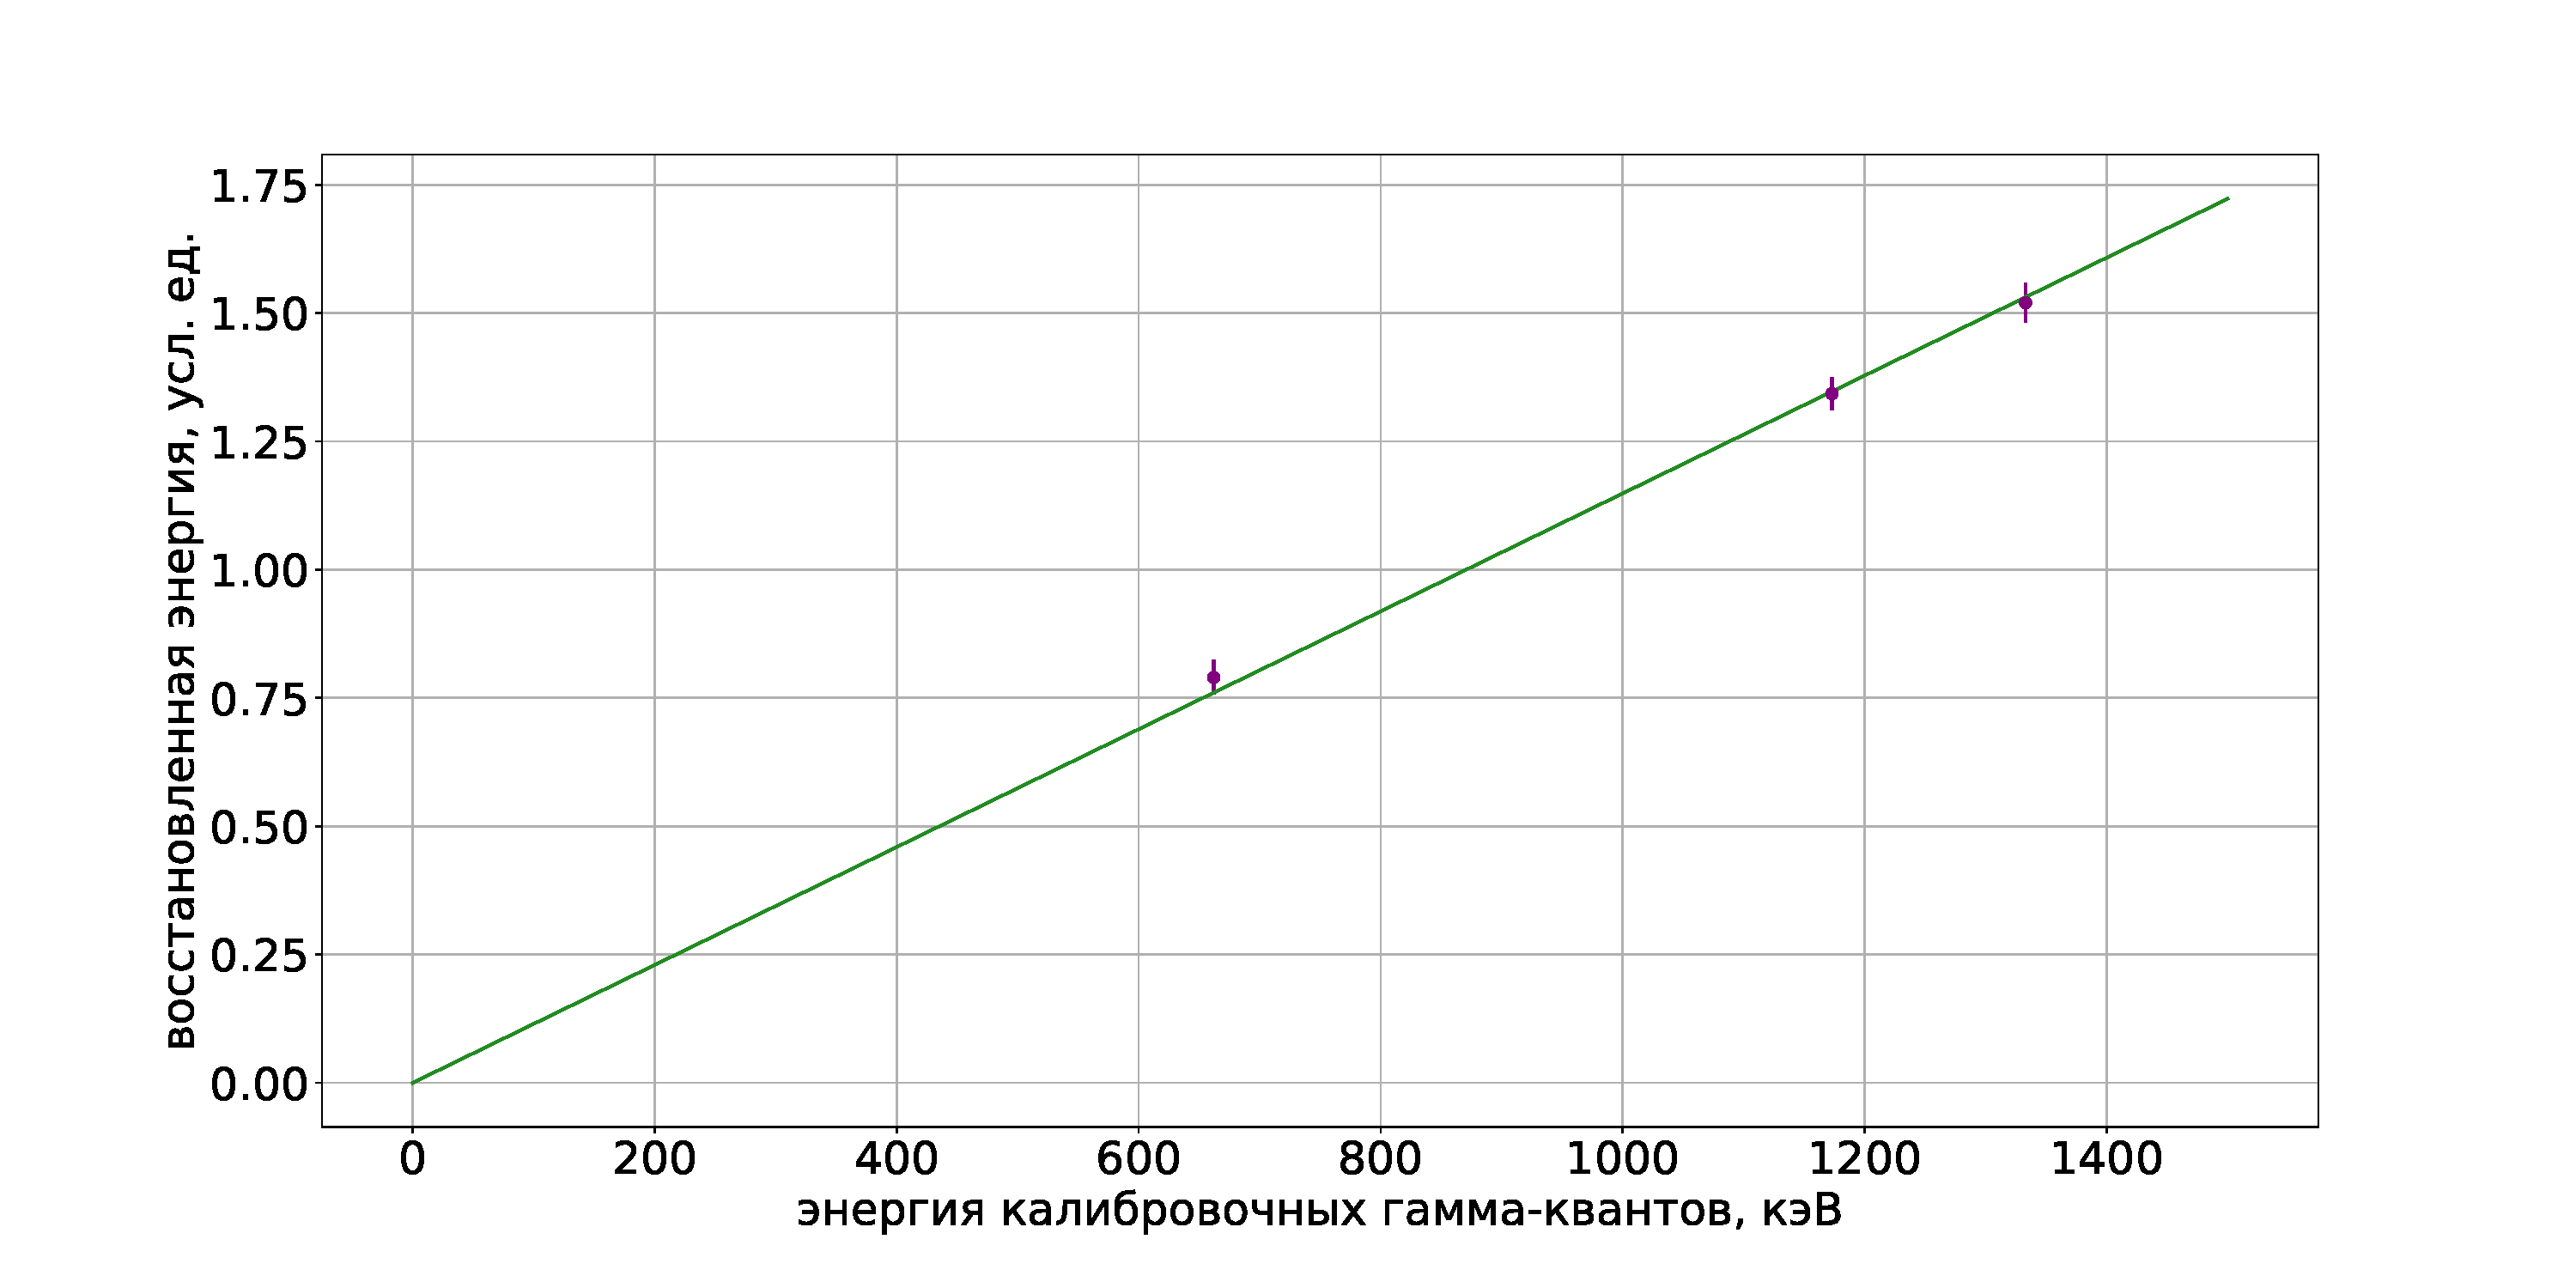
\includegraphics[width=1\linewidth]{images/calibr2022.pdf}}
  \caption{Калибровочный график для сеанса на КАЭС}
  \label{img:calibr2022}  
\end{figure}

\begin{table}[hbt]
    \centering
        \caption{Положения пиков и энергетическое разрешение (сеанс на КАЭС)}
\begin{tabular}{|c|c|c|c|}
\hline
    Энергия, кэВ & Положение пика, кэВ & ($\sigma/E$), \% & FWHM/E,  \%\\
    \hline
    662 & 688$\pm$29 & 8.4 & 19.6\\
    \hline
    1173 & 1169$\pm$27 & 3.7 & 8.7\\
    \hline
    1333 & 1323$\pm$33 & 3.9 & 9.2\\
    \hline
\end{tabular}    
\label{tab:resolution2022}
\end{table}


\section{SE-калибровки}
\label{sect3_4}

Сигналы от одиночных электронов ионизации представляют собой кластеры из равномерно распределенных по времени внутри кластера однофотоэлектронных импульсов. Как уже было упомянуто, SE-данные предсталяют собой формы сигналов в случайные моменты времени. Данные формы сигналов могут содержать как и искомые сигналы, так и совершенно разные события, а также случайные импульсы. Для отбора кластеров импульсов, соответствующих сигналам от одиночных электронов ионизации был применен следующий алгоритм:
\begin{enumerate}
    \itemОтбирались импульсы с амплитудой больше пороговой. Таблица с пороговыми значениями для сеанса на Калининской АЭС приведена в~\ref{AppendixA2}. Пороговые значения вычислялись как $\mu-2\sigma$, где $\mu$ и $\sigma$ -- параметры фита однофотоэлектронного спектра в соответствующем канале.
    \itemОтбирались такие последовательности импульсов, чтобы между любыми двумя из них расстояние было не больше $\Delta T$=500~нс. Величина $\Delta T$ подбиралась экспериментально исходя из знания о том, что длительность кластера, соответствующего электролюминесценции, составляет~$\approx$2~мкс. 
\end{enumerate}

Распределение SE-событий по длительности представлено на рисунке~\ref{img:seduration}. Как и во время сеанса на КАЭС, так и во время инженерного сеанса наблюдались события длительностью существенно меньшей, чем средняя длительность электролюминесценции. Данные события на графиках, представленных на рисунке~\ref{img:seduration}, составляют пик слева от основного. Такие "короткие" события возникают, если электролюминесценция происходит с самого края детектора, где электролюминесцентный зазор ограничен кольцом-держателем сетки. Для дальнейшего анализа данные события были отброшены. Границы отбора по длительности показаны на рисунке~\ref{img:seduration} красными линиями. Распределения суммарного светосбора по данным верхней матрицы для SE-данных представлены на рисунке~\ref{img:sespesp}.
\begin{figure}[H]
  \begin{minipage}[ht]{0.49\linewidth}    \center{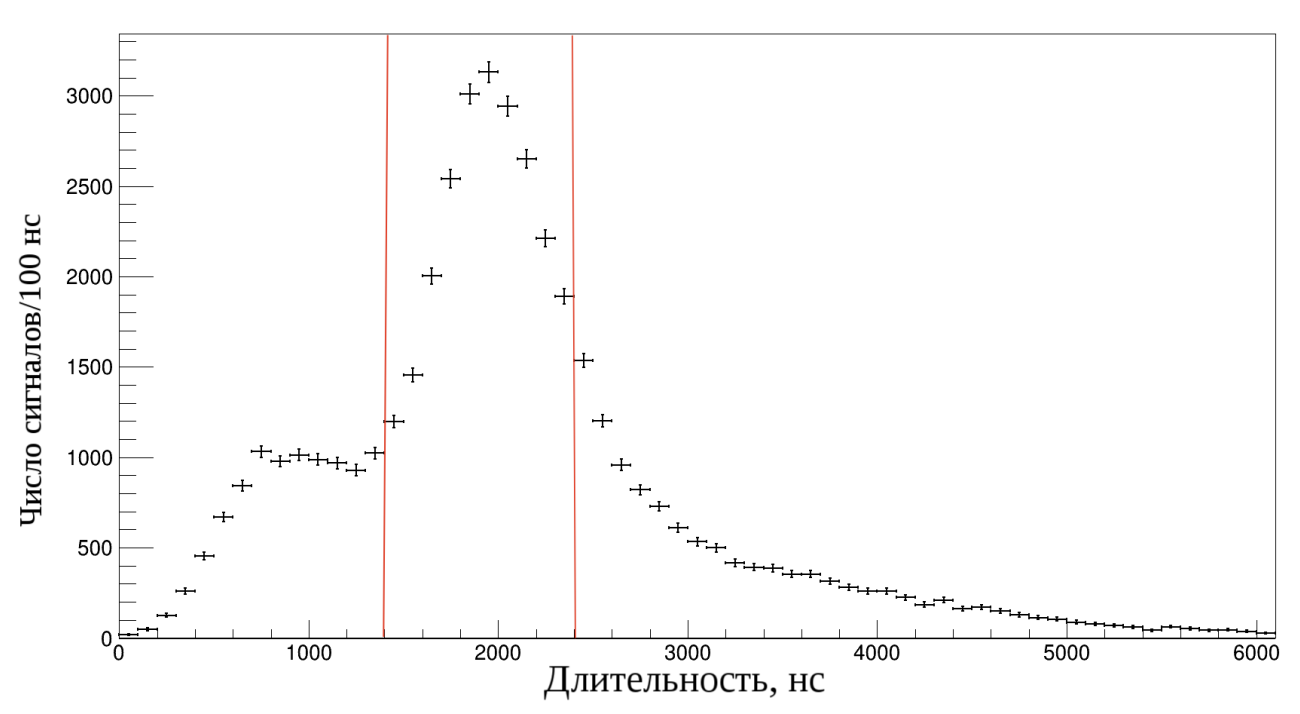
\includegraphics[width=1.0\linewidth]{images/seduration2019.png} \\ а)}
  \end{minipage}
  \hfill
  \begin{minipage}[ht]{0.49\linewidth}  \center{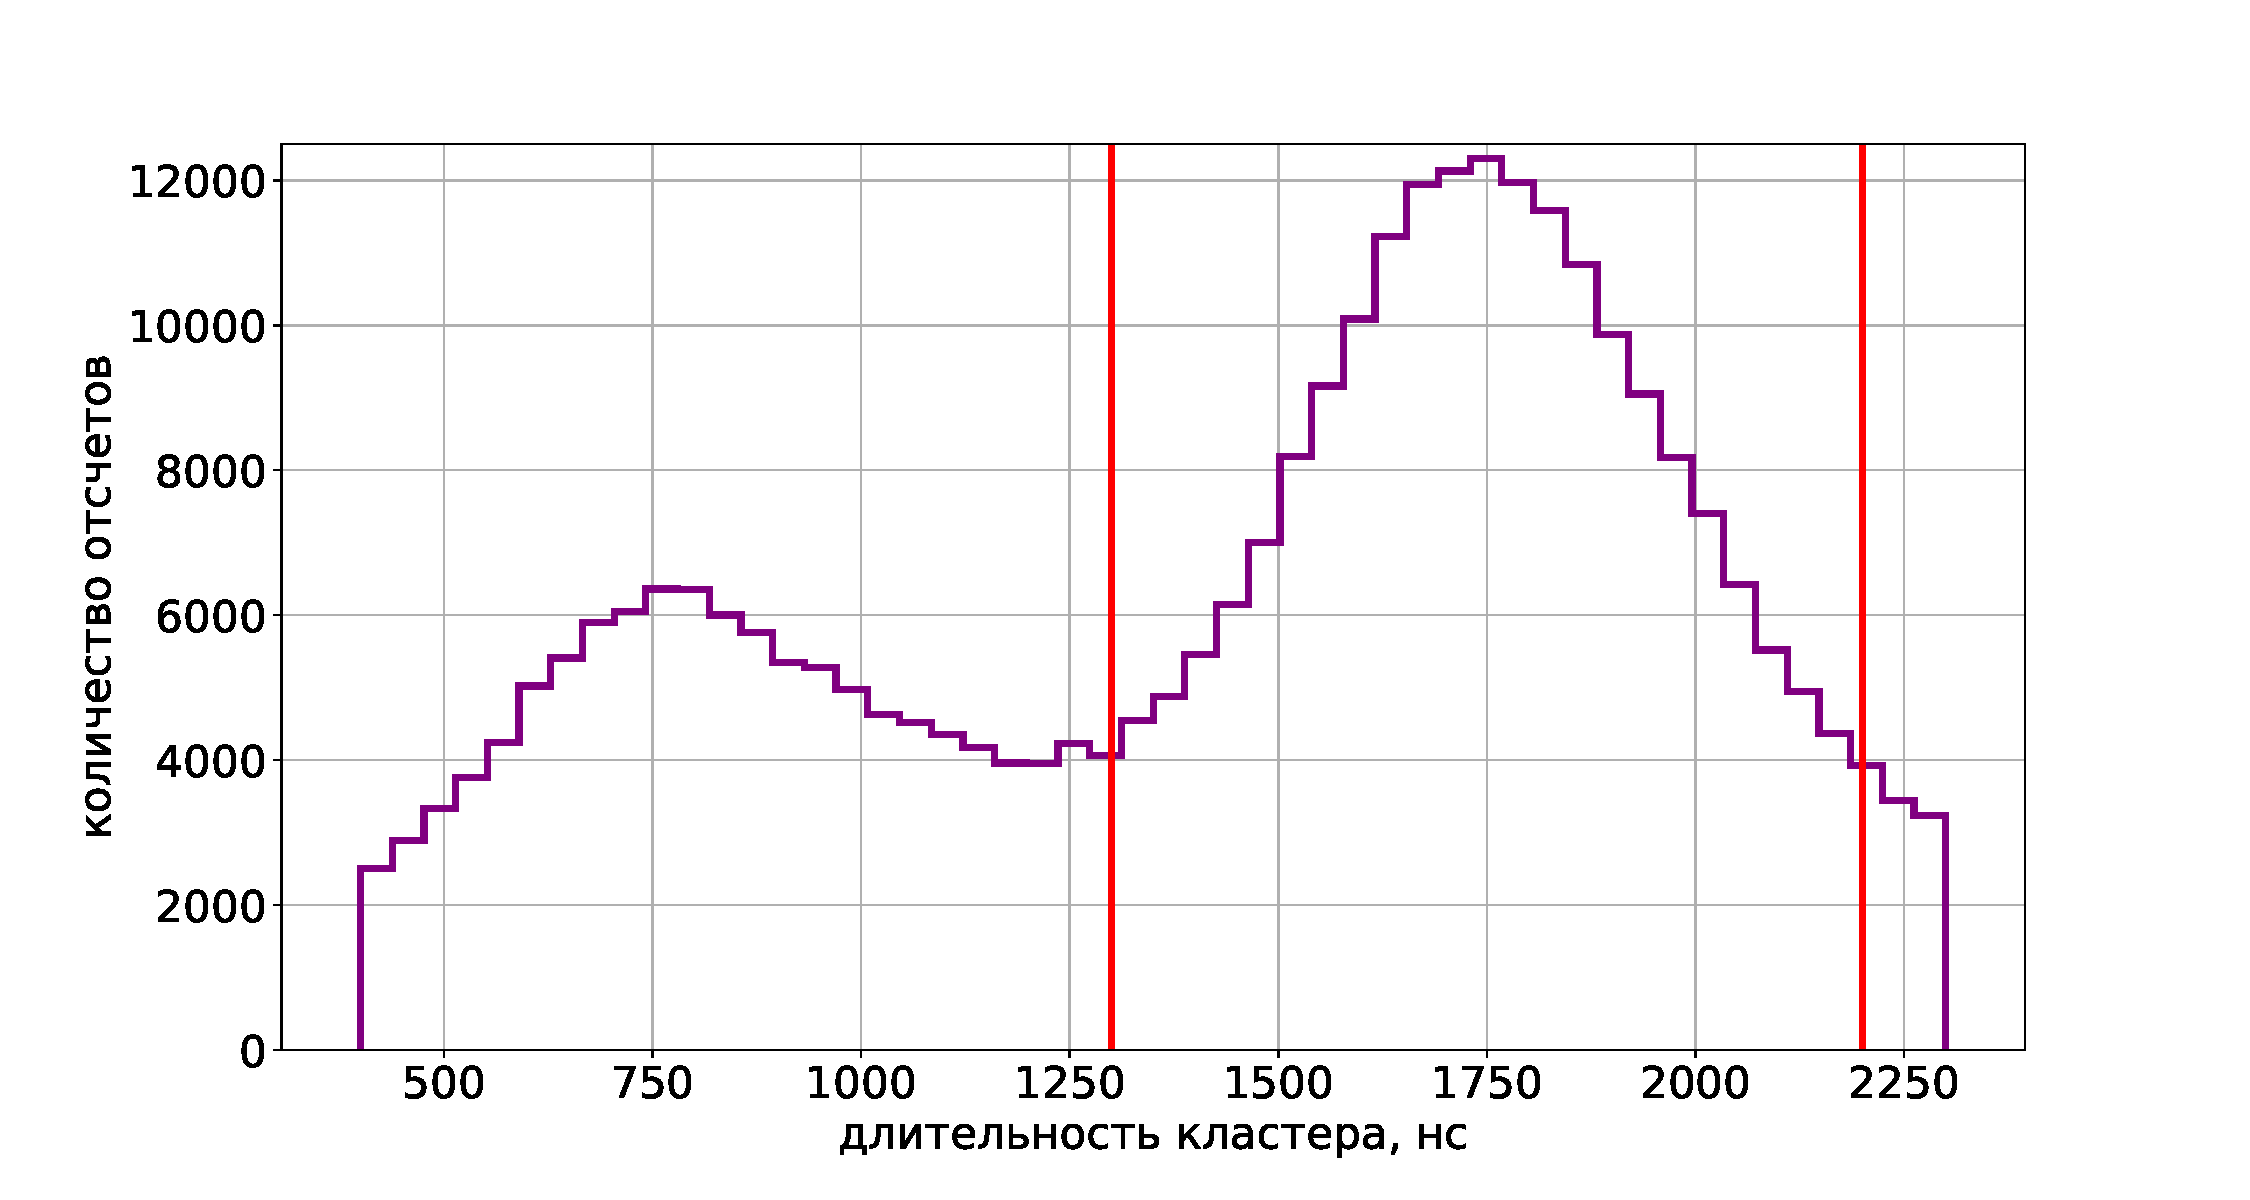
\includegraphics[width=1.0\linewidth]{images/seduration2022.pdf} \\ б)}
  \end{minipage}
  \caption{Распределение событий по длительности для инженерного сеанса (слева) и сеанса на КАЭС (справа)}
  \label{img:seduration}  
\end{figure}

\begin{figure}[H]
  \begin{minipage}[ht]{0.49\linewidth}    \center{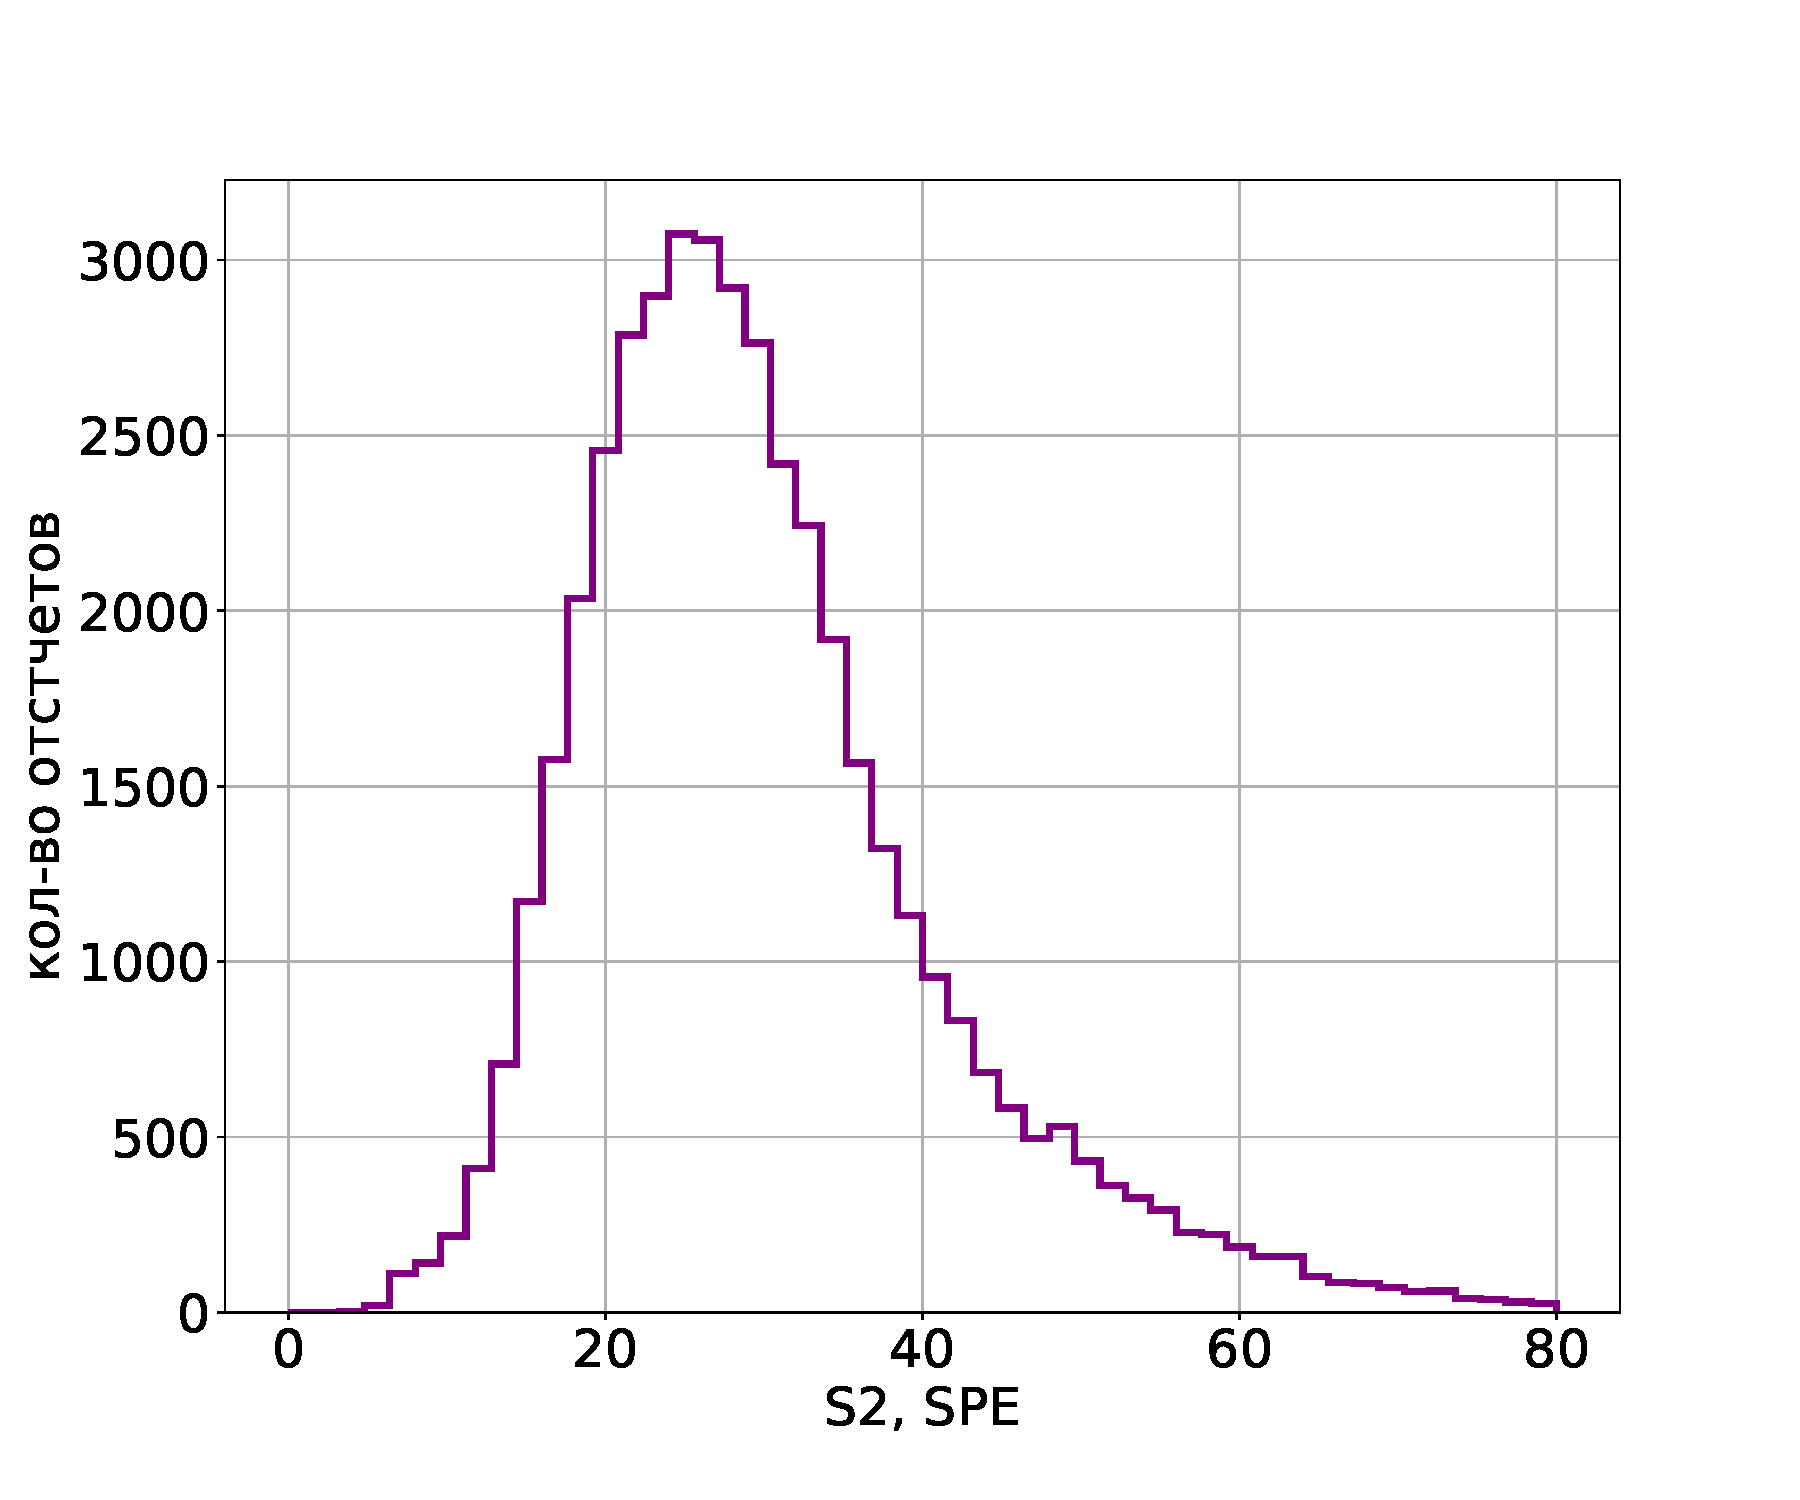
\includegraphics[width=1.0\linewidth]{images/se2019sp.pdf} \\ а)}
  \end{minipage}
  \hfill
  \begin{minipage}[ht]{0.49\linewidth}  \center{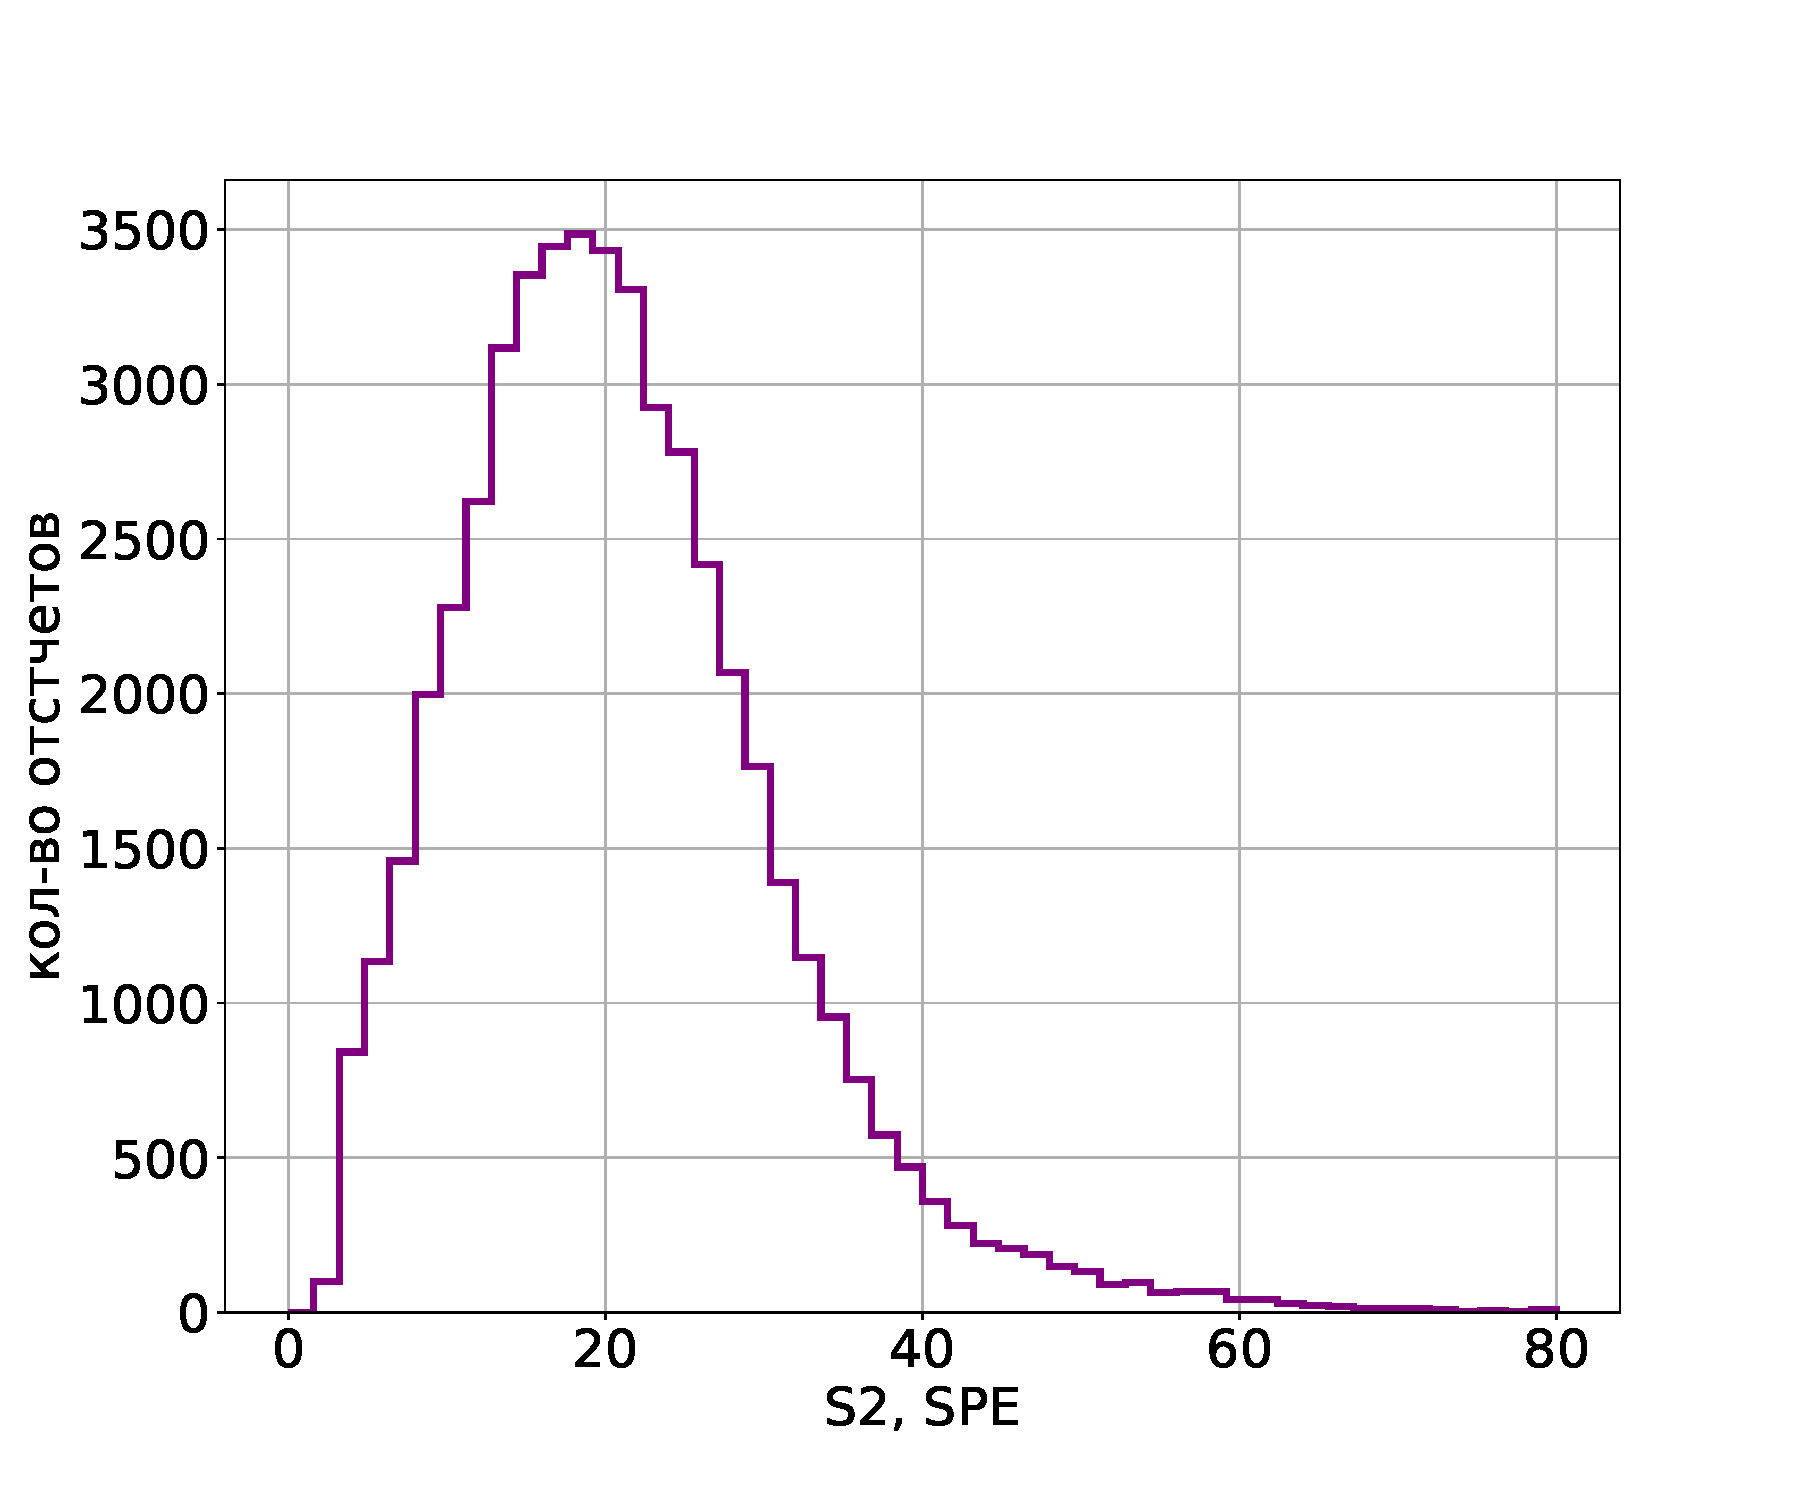
\includegraphics[width=1.0\linewidth]{images/se2022sp.pdf} \\ б)}
  \end{minipage}
  \caption{Распределения S2 в единицах SPE для SE-данных для инженерного сеанса (слева) и сеанса на КАЭС (справа)}
  \label{img:sespesp}  
\end{figure}

\section{Расчет ионизационного выхода и коэффициента экстракции электронов}
\label{sect3_5}
%Для расчета ионизационного выхода требуется величина сигнала от калибровочных гамм в единицах электронов ионизации.
Расчет ионизационного выхода (ionization yield -- IY) производился путем сравнения величины сигнала электролюминесценции от калибровочных гамма-источников и от одиночных электронов ионизации. Соответственно, для данной процедуры требуется выделение одиночного пика калибровочного гамма-источника. Так как разделение пиков $^{60}$Co возможно только в режиме антикорреляции, был использован пик меньшей энергии и данные SE сигналов. Значение ионизационного выхода рассчитывается по формуле:
%мб вместо IY использовать большую фигурную Q
\begin{equation}
    IY = \frac{A_{gamma\:source}}{A_{SE}\cdot E} \qquad \left[ \frac{e^-}{\text{кэВ}} \right]
    \label{formula:IY_calc},
\end{equation} где $A_{gamma\:source}$ и $A_{SE}$ -- положения пиков в фотоэлектронах после процедуры пространственного и энергетического восстановления, a $E$ -- энергия гамма-квантов соответствующего калибровочного источника. Однако, для малых сигналов требуется дополнительная коррекция площади SPE.
%для одиночных SPE для SPE формирующих большую электролюминесценцию имеются различия.
Дело в том, что в импульсах имеется низкоамплитудный хвост, который плохо учитывается в SE-данных, однако, очевидно, вносит вклад при расчете площади событий от калибровочных гамма-источников. Соответственно, требуется коррекция. Форма сигнала SPE для инженерного сеанса и сеанса на КАЭС совпадает, сравнение приведено на рисунке~\ref{img:spe_eff} а).

 Зависимость эффективности вычисления площади SE в зависимости от числа SPE в пачке приведена на рисунке~\ref{img:spe_eff} б). Для данного рассчета моделировались пачки фотоэлектронов с известным количество SPE в каждой и полученной в результате обработки значение количества SPE сравнивалось с изначальным. В связи с этим значение ионизационного выхода, рассчитанное по формуле ~\ref{formula:IY_calc} требуется умножить на соответствующий поправочный коэффициент:
\begin{equation}
    IY = k\cdot  \frac{A_{gamma\:source}}{A_{SE}\cdot E} \qquad \left[ \frac{e^-}{keV} \right]
    \label{formula:IY_calc_corr}
\end{equation}

Значения поправочного коэффициента: %как объяснить разницу если форма одинаковая? оффлайн менялся, и т.д.
\begin{itemize}
    \item ЛЭЯФ: $k = 0.80\pm 0.04$
    \item КАЭС: $k = 0.85\pm 0.03$
\end{itemize}

Значения отличаются для инженерного сеанса и для сеанса на КАЭС, так как были произведены некоторые изменения в параметрах отбора и интегрирования малых импульсов REDOffline.
\begin{figure}[ht]
  \begin{minipage}[ht]{0.49\linewidth}
    \center{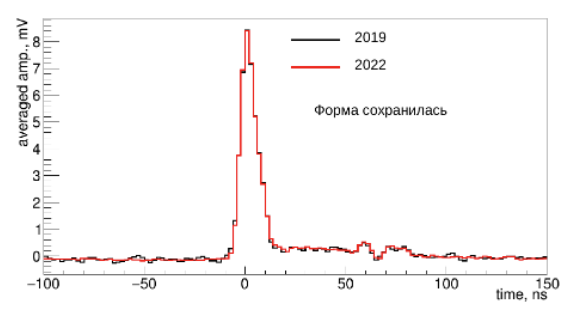
\includegraphics[width=1.0\linewidth]{images/SPE_shape.png} \\ а)}
  \end{minipage}
  \hfill
  \begin{minipage}[ht]{0.49\linewidth}
    \center{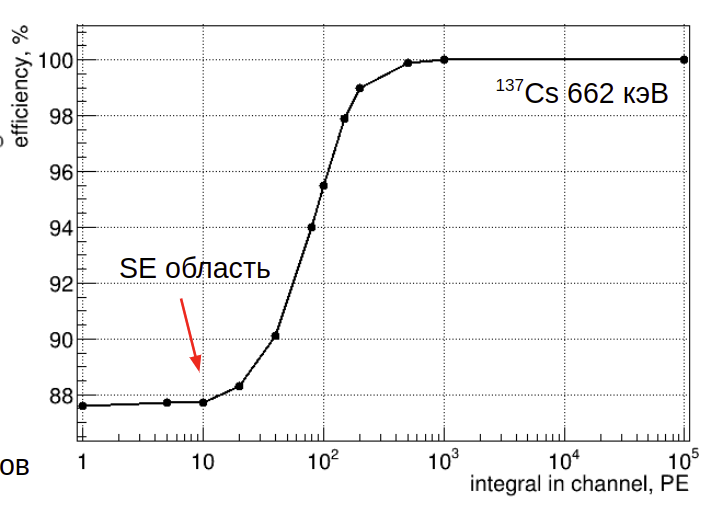
\includegraphics[width=1.0\linewidth]{images/SPE_efficiency.png} \\ б)}
  \end{minipage}
  \caption{а) Сравнение формы сигналов SPE для сеансов 2019 и 2022 гг. б) Зависимость эффективности вычисления площади импульса от количества SPE в импульсе.}
  \label{img:spe_eff}  
\end{figure}

В качестве калибровочного источника, пик от которого присутствует в расчетах, в ЛЭЯФ был использован $^{22}$Na c энергией гамма-квантов 511 кэВ, а при постановке эксперимента на КАЭС -- $^{137}$Cs с энергией гамма-квантов 662 кэВ. Так как расчет коэффициента экстракции электронов важен для предсказания спектра УКРН в детектор, на события был наложен дополнительный отбор на радиус от центра детектора (155 мм для инженерного сеанса и 130 мм для сеанса на КАЭС). Отбор событий, набранных во время сеанса на КАЭС совпадает с отбором, применявшимся для анализа УКРН-событий. Спектры S2 для гамма-калибровочных событий и для SE событий фитировались распределениями Гаусса для получения положений пиков. Калибровочные спектры на рисунке~\ref{img:NaCsfit}. SE спектры приведено на рисунке~\ref{img:SEfit}.

\begin{figure}[H]
  \begin{minipage}[ht]{0.49\linewidth}
    \center{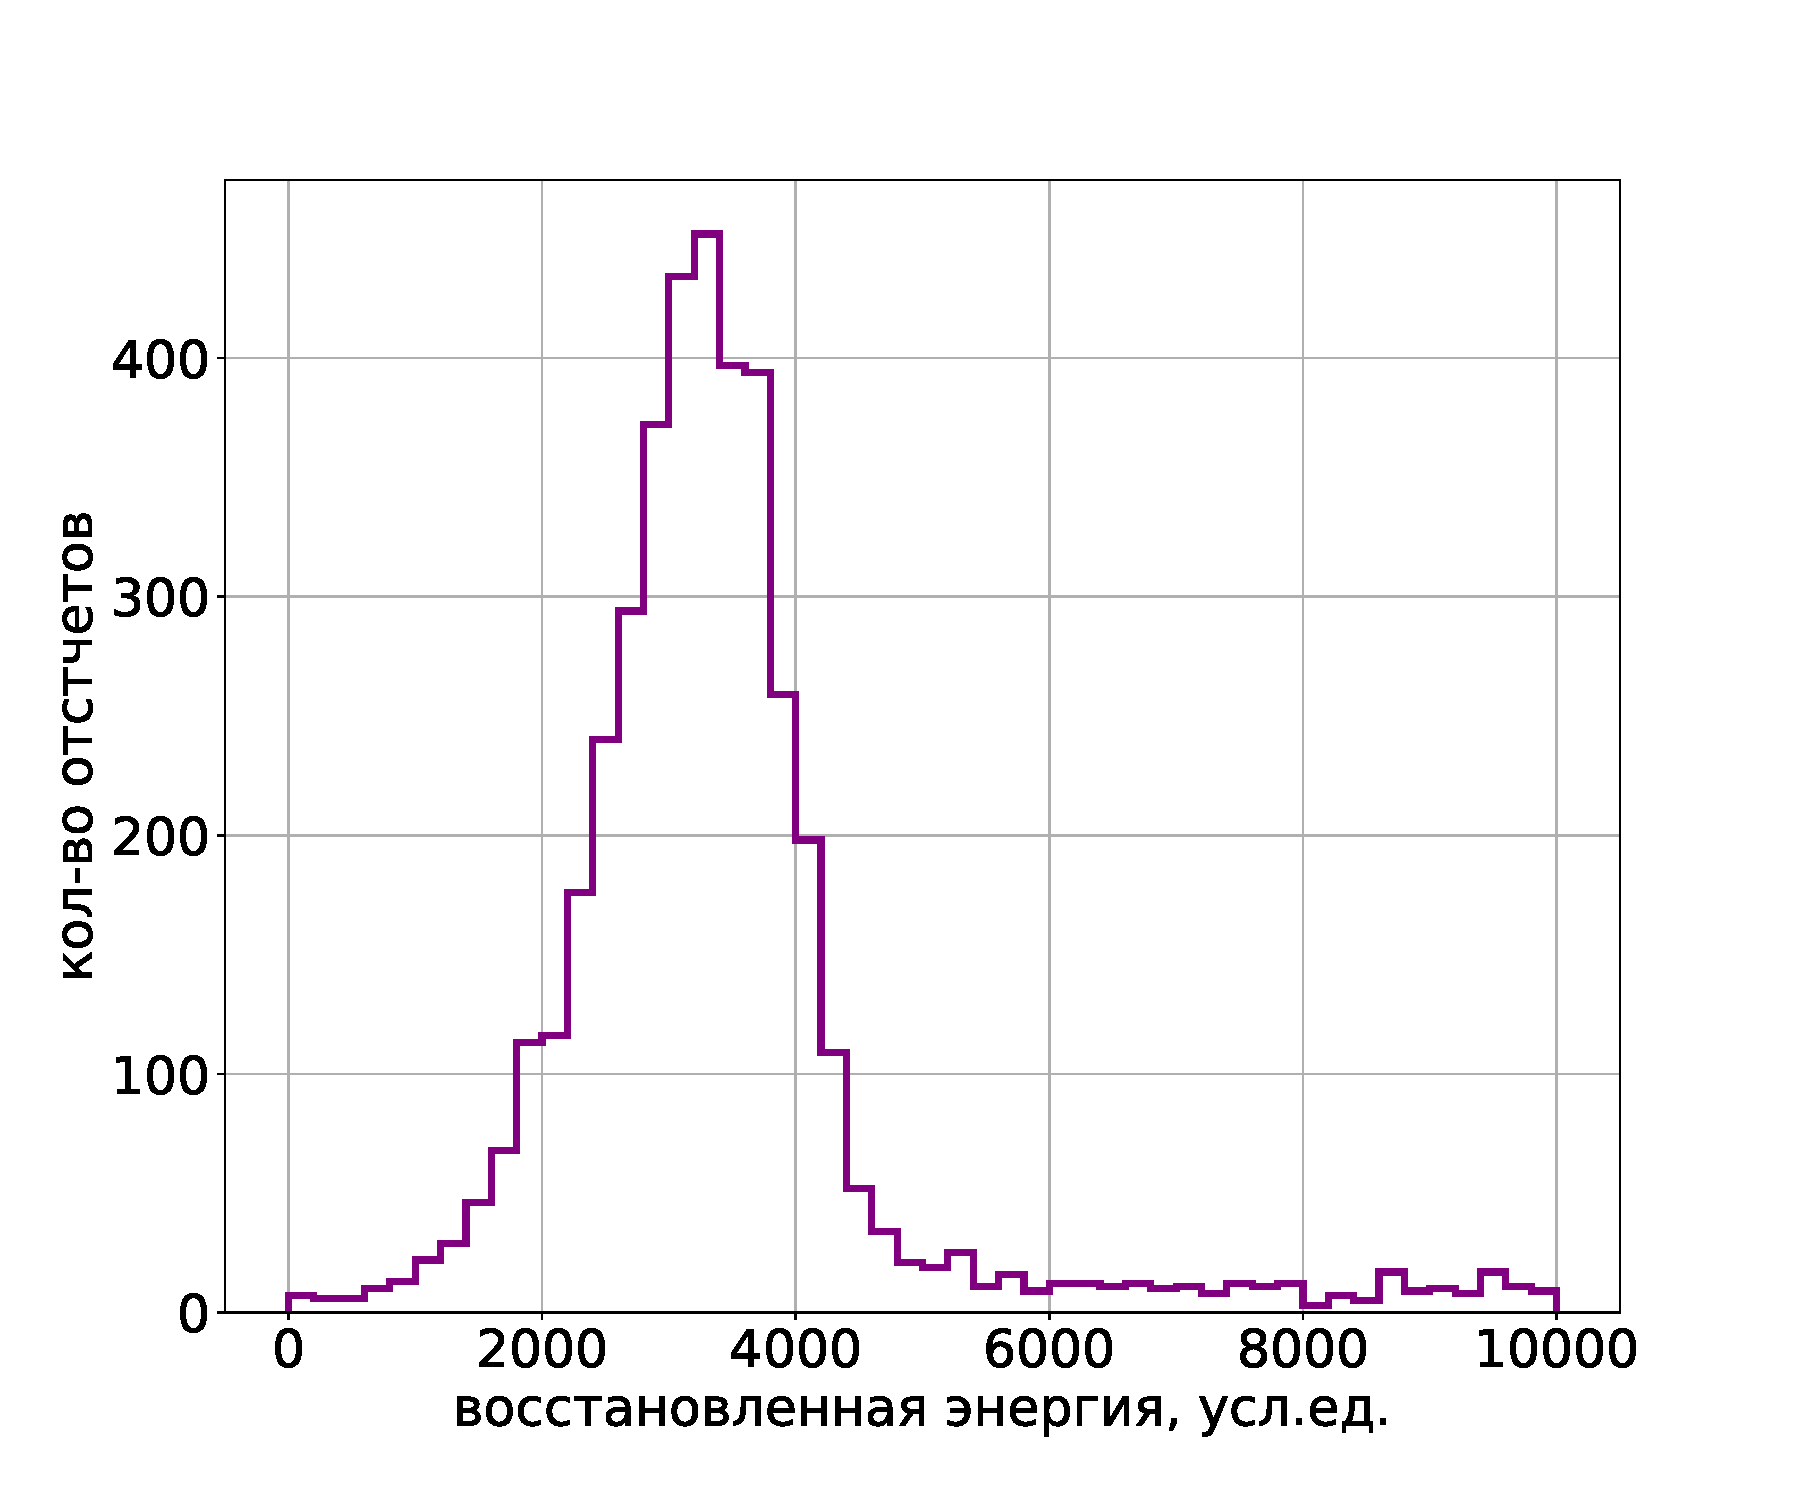
\includegraphics[width=1.0\linewidth]{images/na2019recsp.pdf} \\ а)}
  \end{minipage}
  \hfill
  \begin{minipage}[ht]{0.49\linewidth}
    \center{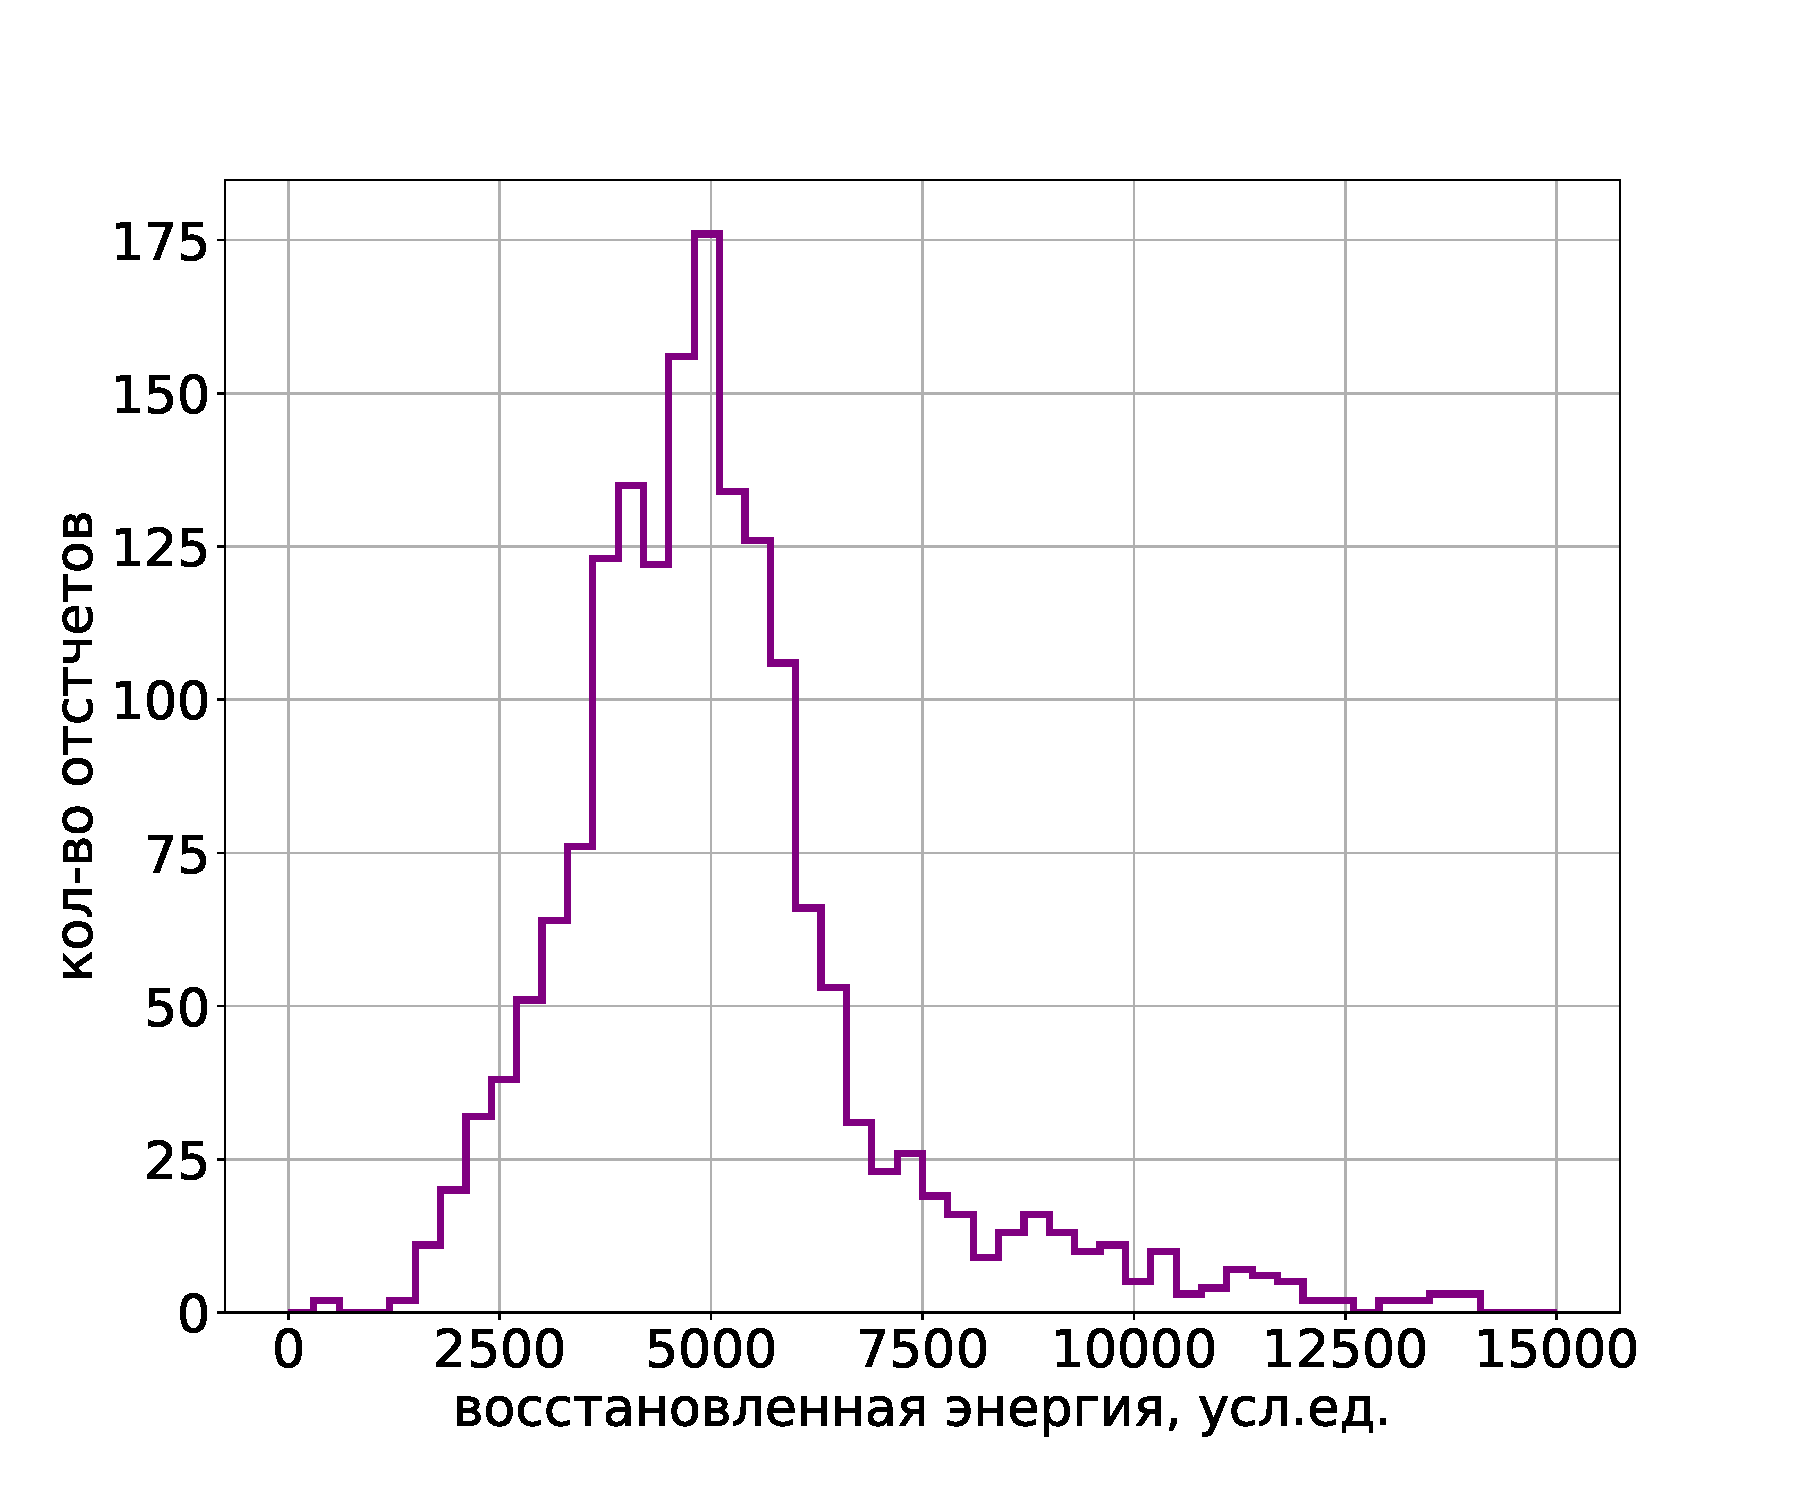
\includegraphics[width=1.0\linewidth]{images/cs2022recsp.pdf} \\ б)}
  \end{minipage}
  \caption[Спектры восстановленной энергии S2 для калибровочных источников]{а) Спектр восстановленной энергии S2 для $^{22}$Na (инженерный сеанс) б) Спектр восстановленной энергии S2 для $^{137}$Cs (сеанс на КАЭС)}
  \label{img:NaCsfit}  
\end{figure}

\begin{figure}[H]
  \begin{minipage}[ht]{0.49\linewidth}
    \center{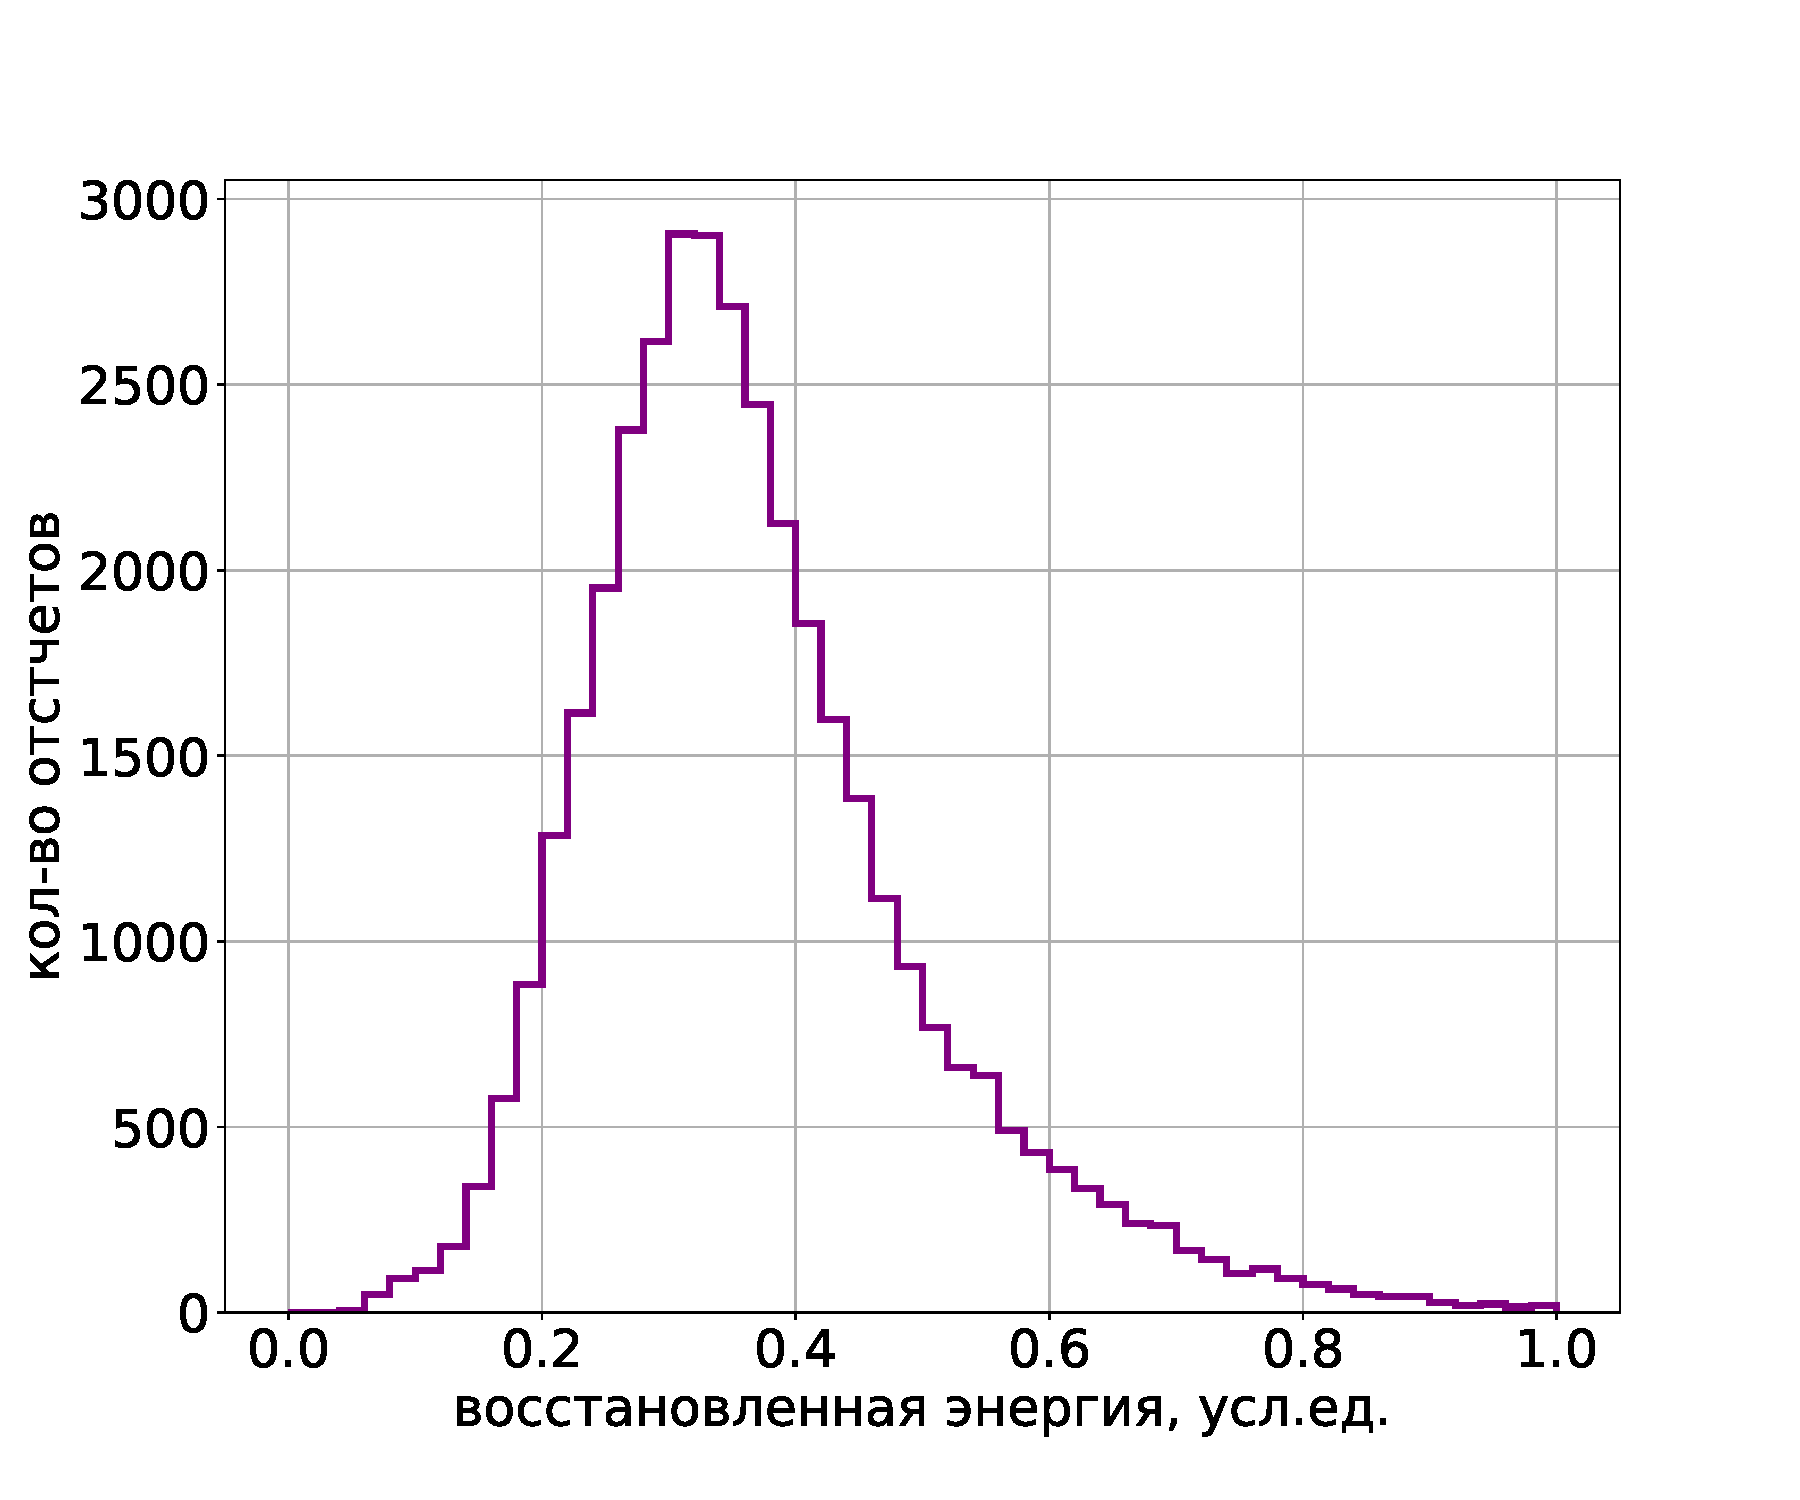
\includegraphics[width=1.0\linewidth]{images/se2019recsp.pdf} \\ а)}
  \end{minipage}
  \hfill
  \begin{minipage}[ht]{0.49\linewidth}
    \center{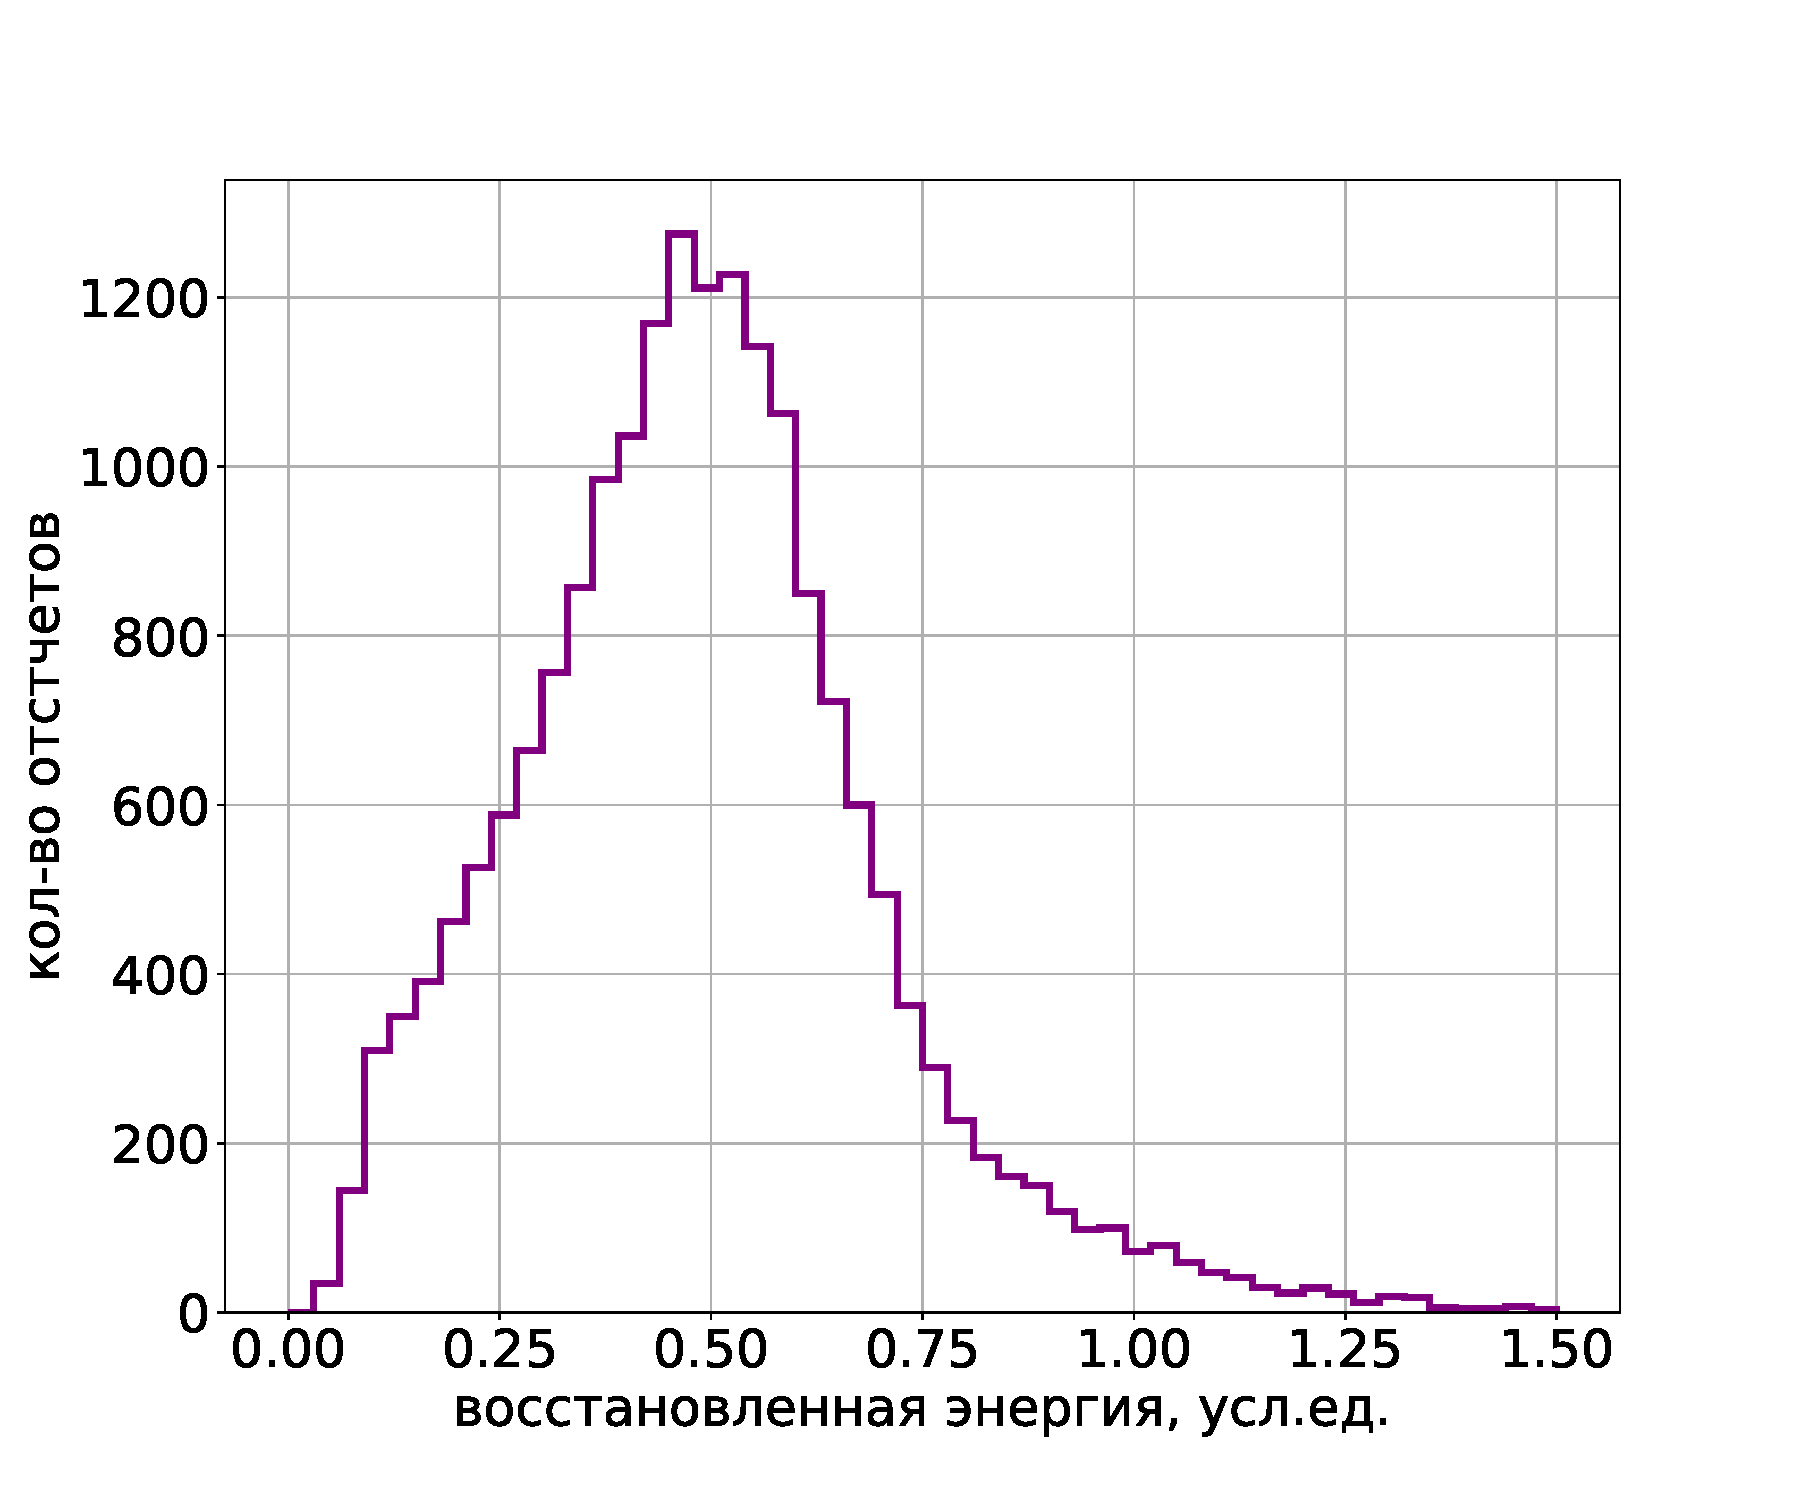
\includegraphics[width=1.0\linewidth]{images/se2022recsp.pdf} \\ б)}
  \end{minipage}
  \caption[спектры восстановленной энергии S2 для SE-данных]{а) Спектр восстановленной энергии S2 для SE (инженерный сеанс) б) Спектр восстановленной энергии S2 для SE (сеанс на КАЭС)}
  \label{img:SEfit}  
\end{figure}

\parОсновная идея рассчета коэффициента экстракции электронов состоит в сравнении количества рожденных электронов в месте взаимодействия гамма-кванта с веществом и количества зарегистрированных электронов ионизации по S2. 
Значения величин ионизации для соответствующих энергий, были рассчитаны с использованием программного пакета NEST %версия?. 
\parПолученные значения ионизационного выхода и коэффициента экстракции электронов:
\begin{itemize}
    \item 2019: IY = 15.6$\pm$0.7 e/keV, EEE = 38$\pm$6.1\%
    \item 2022: IY = 12.9$\pm$0.7 e/keV, EEE = 34$\pm$5.9\%
\end{itemize}

Было произведено сравнение полученных значений с измерениями других коллабораций~\cite{Gouschin1978,AprileEEE_2014,Edwards_2018,PhysRevD.99.103024}. Результаты представлены на рисунке \ref{img:EEEworld}. Также на данном рисунке представлен расчет с использованием программного пакета NEST. Результаты, полученные в эксперименте РЭД-100 имеют тенденцию к отличию в большую сторону от общемировых значений. Вероятно, это связано с недостаточной точностью при расчете электрических полей в электролюминесцентном зазоре.

\begin{figure}[H]
\center{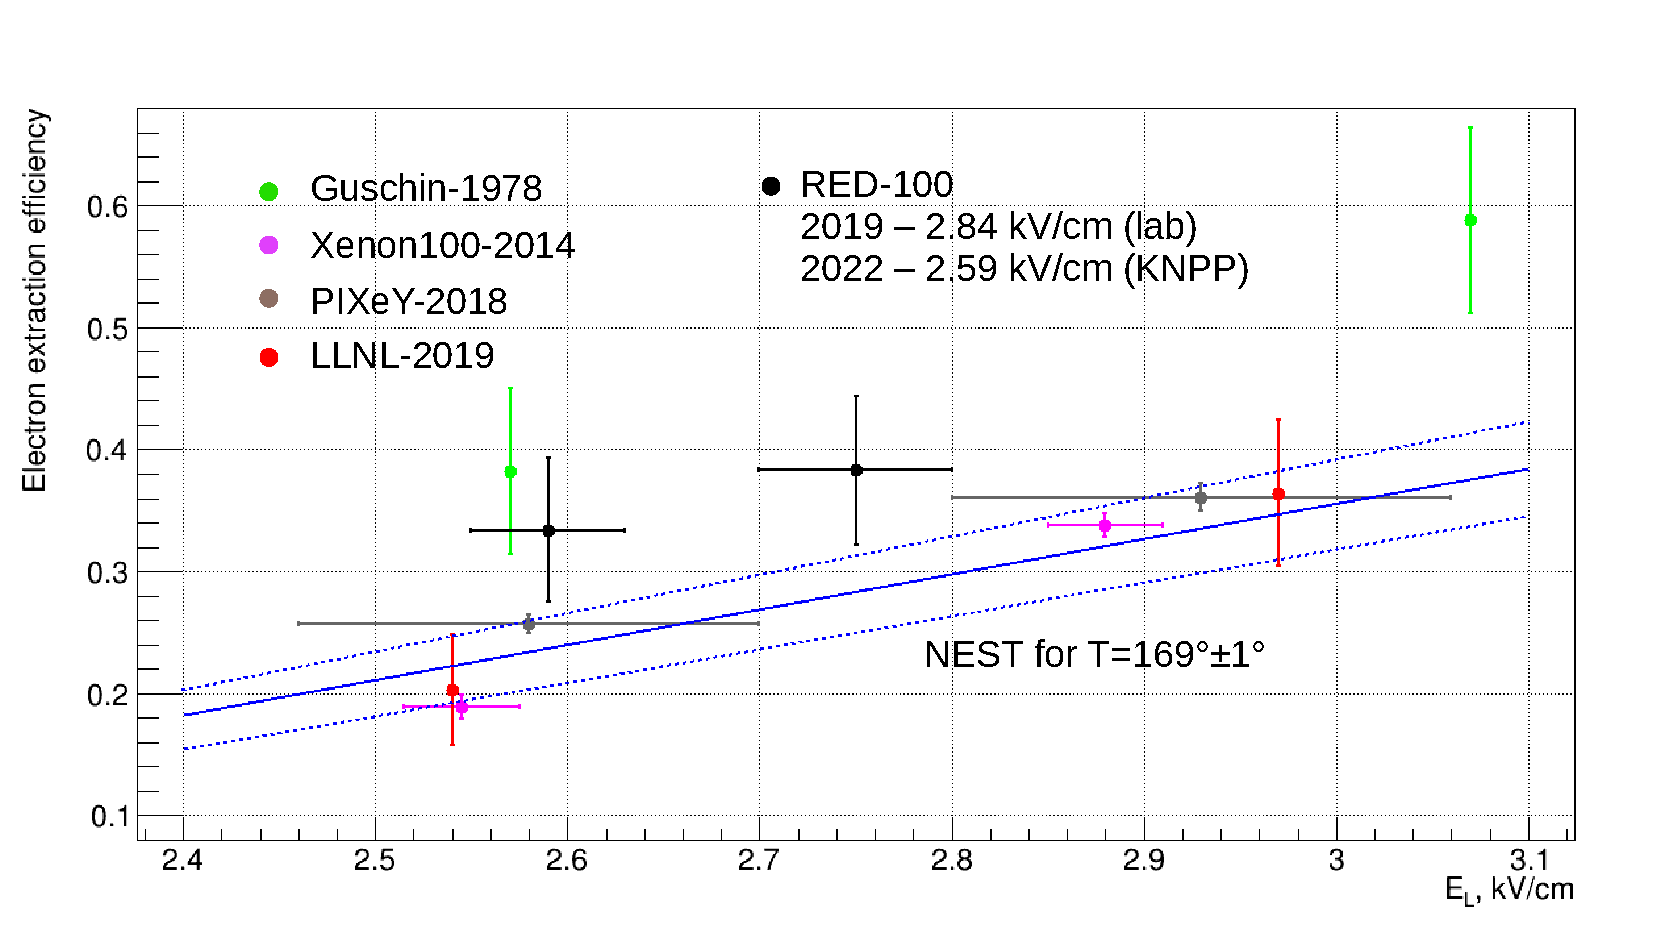
\includegraphics[width=1\linewidth]{images/RED_EEE_With_legend.pdf}}
  \caption{Сравнение результатов измерения ЕЕЕ в эксперименте РЭД-100 и другими коллаборациями, а также резульаты расчета данного коэффициента с использованием программного пакета NEST.}
  \label{img:EEEworld}  
\end{figure}           % Глава 3
\chapter{Анализ физических данных эксперимента РЭД-100 на Калининской АЭС} 
\label{chapt4}
Для увеличения достоверности результатов, проводился так называемый слепой анализ. Все методы обработки и анализа в данном случае отрабатываются на фоновых данных (набранных при выключенном реакторе), и только после полного понимания всех процедур допускается их применение к данным, набранным со включенным реактором без изменений.
\section{Моделирование УКРН событий}
\label{sect4_1}
Важным этапом при анализе данных эксперимента является детальное понимание отклика детектора на сигнальные события. Для эксперимента РЭД-100 на КАЭС сигнальными событиями являются события от УКРН. 

Учитывая известную мощность реактора моделировался энергетический спектр ядер отдачи в GEANT-модели детектора, который далее пересчитывался в спектр, выраженный в электронах ионизации. При дрейфе и экстракции с поверхности электроны ионизации претерпевают потери, которые были рассчитаны с использованием полученных в \ref{sect3_1} и \ref{sect3_5} значений времени жизни электронов в жидком ксеноне и коэффициента экстракции, соответственно. Спектр до и после данных потерь представлен на рисунке \ref{img:cevnscpectrum}.
\begin{figure}[H]	
\center{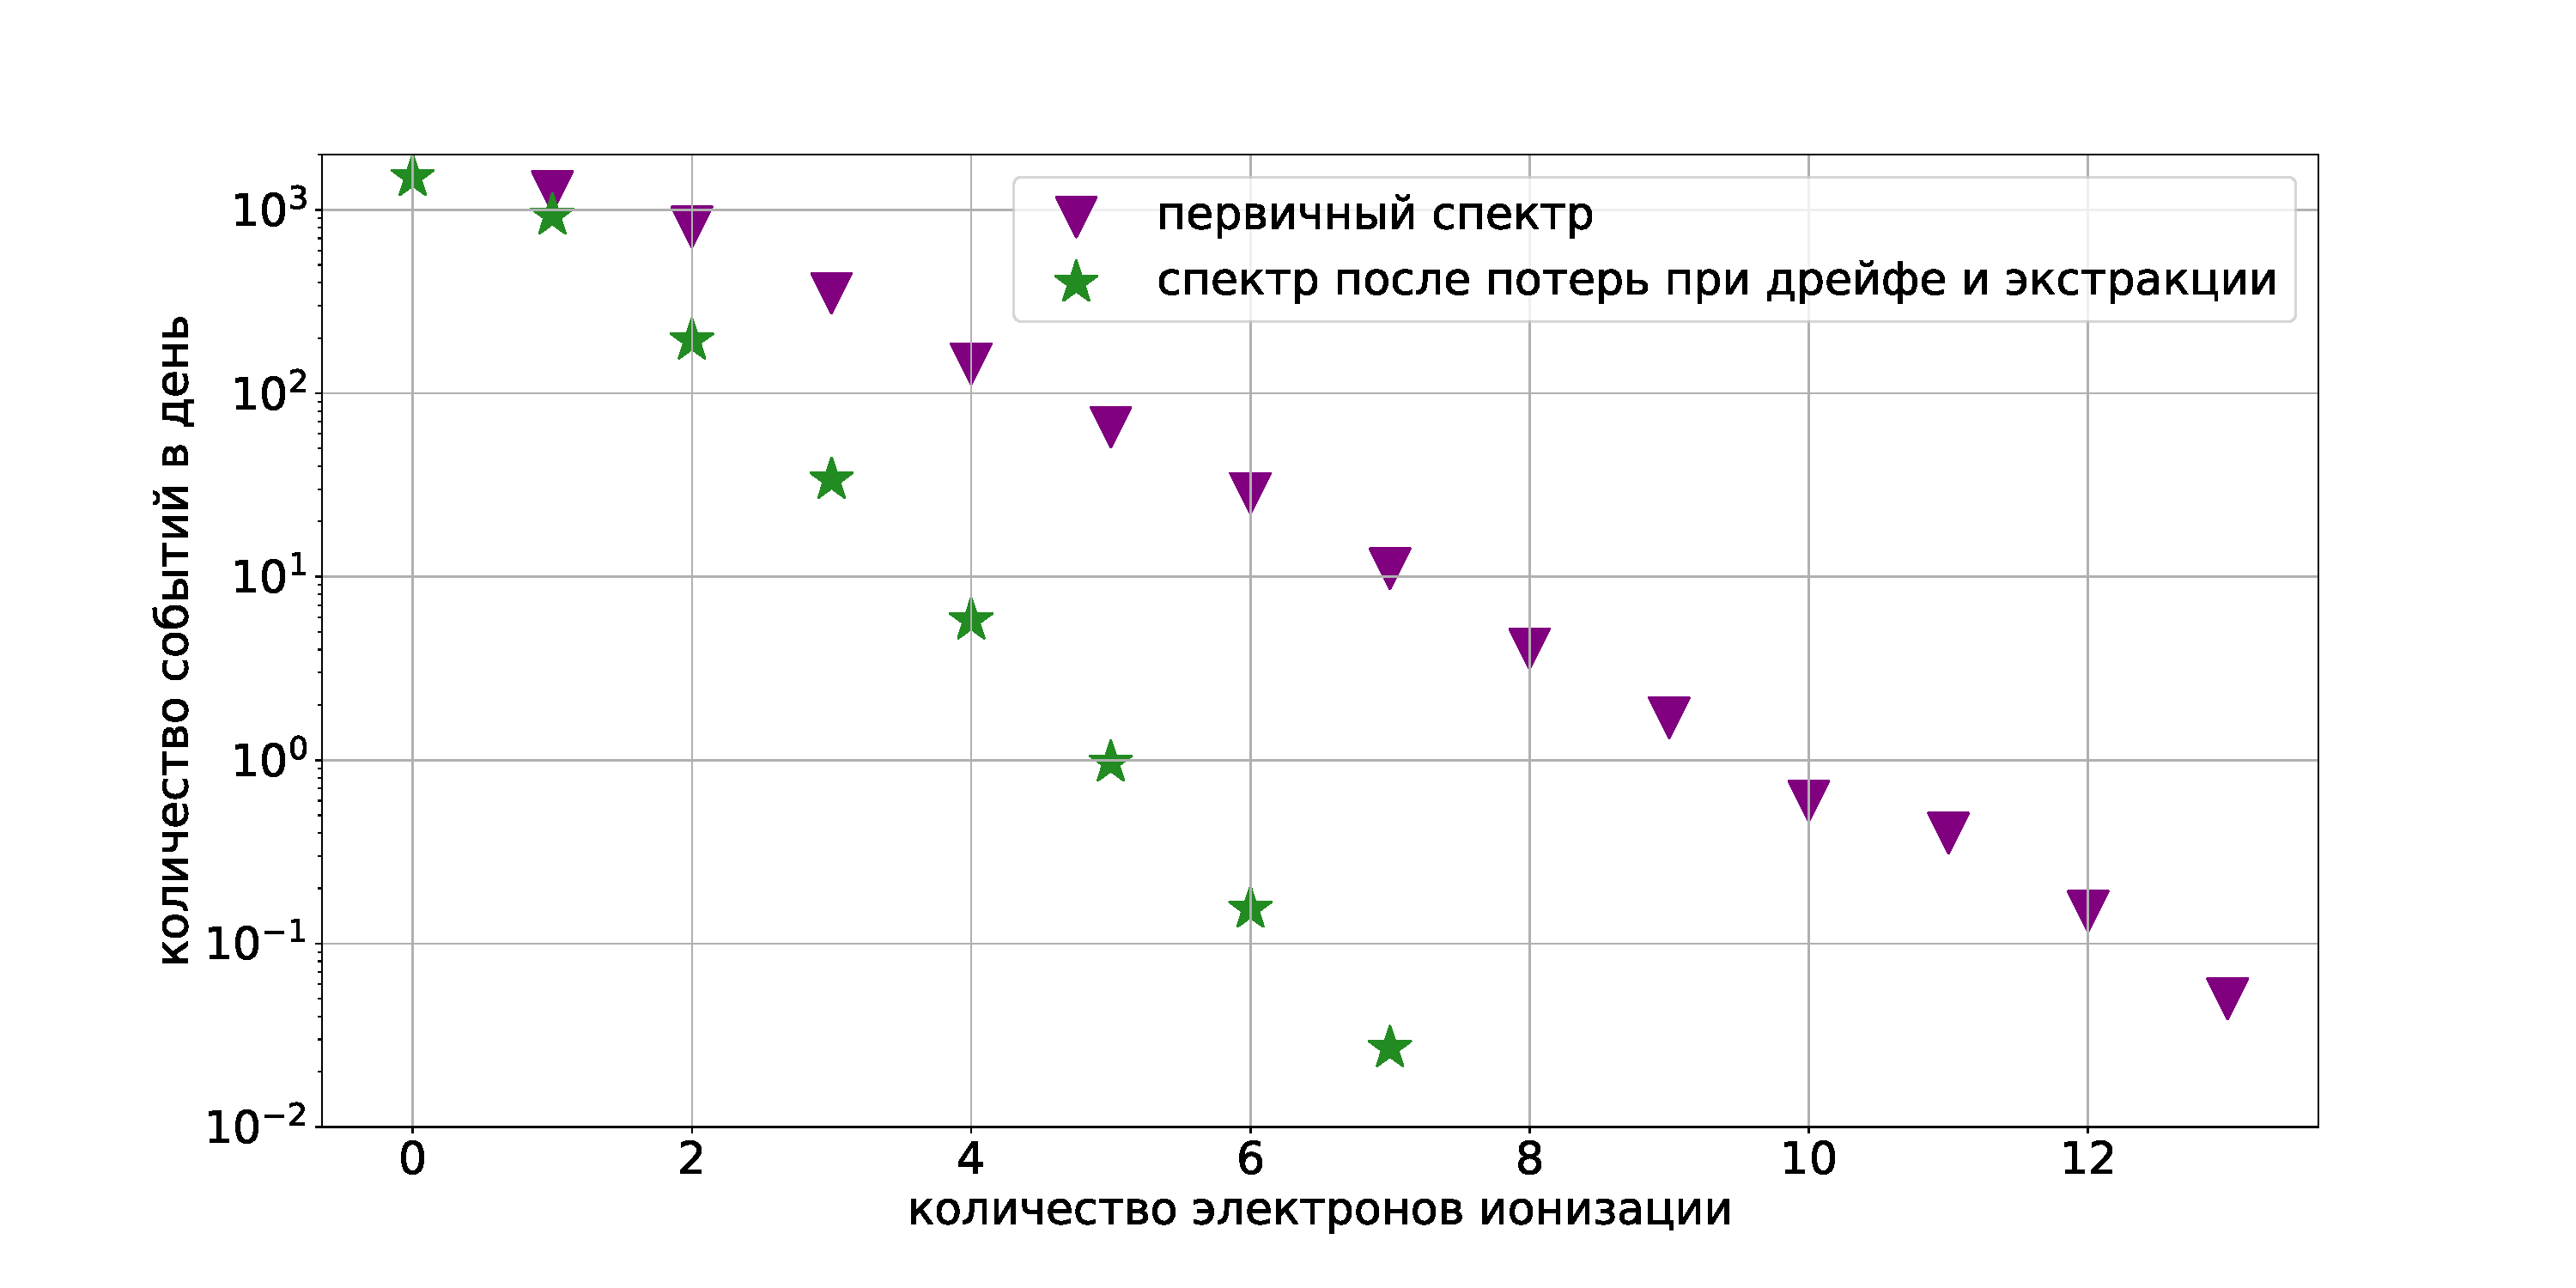
\includegraphics[width=1.0\linewidth]{images/cevnsspectrumSE.pdf}}
	\caption{Смоделированный спектр УКРН-событий, выраженный в электронах ионизации, до и после потерь при дрейфе и экстракции.}
	\label{img:cevnscpectrum}
\end{figure}

Далее, в соответствии с описанной в \ref{subsect2_3_2} процедурой были смоделированы события в несколько электронов ионизации согласно полученному спектру. При моделировании использовались LRF, полученные при анализе измерений с гамма-источниками. Также была проведена процедура реконструкции координат и энергии данных событий. Для улучшения соотношения сигнал/шум при дальнейшем анализе к событиям были применены дополнительные отборы по длительности (<5 мкс) и радиусу (<130 мм), совпадающие с отборами для экспериментальных данных. Результирующий спектр восстановленной энергии смоделированных УКРН-событий представлен на рисунке \ref{img:cevnscpectrumspe}. 
\begin{figure}[H]
\center{\includegraphics[width=1.0\linewidth]{images/cevnsspectrumSPE.pdf}}
	\caption{Спектр восстановленной энергии смоделирванных УКРН-событий.}
	\label{img:cevnscpectrumspe}
\end{figure}


\section{Кластеризация и отбор экспериментальных данных}
\label{sect4_2}
При наборе ME-данных использовался триггер, описанный в~\ref{subsect2_1_3}, позволяющий записывать события в несколько электронов ионизации. На записанных формах сигнала выделялись следующие диапазоны:
\begin{itemize}
    \itemОбласть перед триггером: от 0 до 15 мкс
    \itemОбласть триггера: от 17.5 до 20.5 мкс
    \itemОбласть после триггера: от 22 мкс до 30 мкс
\end{itemize}

Первичный отбор кластеров событий в несколько электронов ионизации (ME -- Multiple Electrons) аналогичен соответствующей процедуре для SE-событий (см~\ref{sect3_4}). Отличие заключалось в выборе пороговых значений для отбора импульсов, связанное с изменением SPE-калибровки. Таблица с пороговыми значениями представлена в~\ref{AppendixA3}. Кроме того, на события были наложены дополнительные отборы, учитывающие форму сигнала:
\begin{itemize}
    \item нет отсчетов, отклоняющихся в противоположную сигналу сторону более чем на 10~мВ (данный отбор обеспечивает защиту от так называемого "звона" в каналах)
    \item в кластере присутствует не менее 20 импульсов
    \item начало кластера находится в области триггера или начало находится до области триггера, а конец -- после
    \item для каждого импульса отношение характерного заряда SPE в соответствующем канале к амплитуде импульса больше порогового значения в 2.0 (данный отбор обеспечивает защиту от наличия высокоамплитудных одиночных импульсов, которые могут возникать как от сцинтилляции, так и от черенковского излучения)
    \item отношение суммарной площади импульсов в окрестности ([-20,+180]~нс) самого большого импульса кластере к полной сумме всех импульсов кластера меньше порогового значения 0.4 (цель данного отбора аналогична цели предыдущего)
    \item отношение площади импульсов внутри интервала длительностью 1 мкс, находящегося внутри кластера и дающего максимальный вклад в суммарную площадь, к общей площади импульсов кластера меньше порогового значения 0.84 (данный отбор позволяет бороться с событиями, внутри которых наблюдается существенное отклонение от равномерности распределения импульсов по времени внутри кластера)
    \item длительность кластера составляет от 1.6 до 5.0 мкс
    \item в области перед триггером находится менее 50 импульсов
    \item в области после триггера находится менее 35 импульсов
    \item восстановленный при помощи LRF радиус меньше 130~мм
\end{itemize}

Пример суммарной формы сигнала события, прошедшего все отборы, представлен на рисунке~\ref{img:event_example}.
\begin{figure}[H]
\center{\includegraphics[width=0.8\linewidth]{images/pic_run0520_file0002_ev1049.png}}
	\caption{Пример суммарной формы сигнала события, прошедшего все отборы.}
	\label{img:event_example}
\end{figure}

Как уже упоминалось в \ref{subsect2_1_5}, существенную часть фона составляет совпадающие по времени сигналы от одного или нескольких спонтанно возникших электронов ионизации, как показано на рисунке~\ref{img:overlap}.
\begin{figure}[H]
\center{\includegraphics[width=0.5\linewidth]{images/randomoverlap.png}}
	\caption{Иллюстрация механизма возникновения событий совпадения.}
	\label{img:overlap}
\end{figure}

Для борьбы с такими событиями можно использовать идею о том, что точечные события не могут давать множественные вершины на плоскости XY. С целью подавления данной компоненты фона были применены технологии машинного обучения, а именно были разработаны две нейронные сети. Обучение сетей производилось на смоделированных событиях.
Точечные события для обучения нейронных сетей моделировались по такому же принципу, как и события УКРН. События совпадения конструировались из двух или более точечных событий, произошедших в одно время, но в разных местах на плоскости XY.

Первая нейронная сеть представляет собой полносвязный перцептрон~\cite{perceptron}, который в качестве входных данных использует только распределение света по верхней матрице ФЭУ, без учета времени возникновения сигналов.

Вторая нейронная сеть помимо полносвязных слоев имеет в своем составе сверточные~\cite{INDOLIA2018679} и принимает на вход псевдо-изображение 19х19 пикселей, где по вертикальной откладывался номер ФЭУ, а по горизонтальной оси -- время регистрации фотонов. Числовое значение в каждом пикселе соответствовало количеству зарегистрированных фотонов в конкретном канале в конкретный бин по времени. Примеры описанных выше изображений приведены на рисунке~\ref{img:cevnsbckgevents}. Анализ подобных псевдо-изображений применялся для восстановления координат и энергии в работе~\cite{Delaquis_2018}. 

Результаты отбора УКРН событий и подавления фона, расчитанные по смоделированным данным приведены в таблицах~\ref{NNeffcevns}~и~\ref{NNeffbckg}. Для дальнейшего анализа отбирались события, идентифицированные обеими сетями как точечные.

\begin{figure}[ht]
  \begin{minipage}[ht]{0.49\linewidth}    \center{\includegraphics[width=1.0\linewidth]{images/cevns_event_6SE_1206_0.pdf} \\ а)}
  \end{minipage}
  \hfill
  \begin{minipage}[ht]{0.49\linewidth}  \center{\includegraphics[width=1.0\linewidth]{images/bckg_event_6SE_1206_5.pdf} \\ б)}
  \end{minipage}
  \caption[Пример временных разверток смоделированных событий, применявшихся для тренировки нейросетей для отбора по точечности.]{Пример временных разверток смоделированных событий, применявшихся для тренировки нейросетей для отбора по точечности. a) -- точечное событие в 6 электронов ионизации, б) -- "неточечное" событие, состоящее из нескольних отдельных событий, в сумме дающих 6 электронов ионизации}
  \label{img:cevnsbckgevents}  
\end{figure}

\begin{table}[H]
    \centering
    \caption{Эффективности прохождения УКРН-событий для каждой из сетей, расчитанные по смоделированным данным.}  
\begin{tabular}{|c|c|c|c|c|}
\hline Количество SE & 3 & 4 & 5 & 6 \\
\hline сверточная сеть & $0.93$ & $0.96$ & $0.97$ & $0.98$ \\
\hline перцептрон & $0.88$ & $0.91$ & $0.93$ & $0.94$ \\
\hline
\end{tabular}
\label{NNeffcevns}
\end{table}

\begin{table}[H]
    \centering
    \caption{Эффективности подавления фоновых событий для каждой из сетей, расчитанные по смоделированным данным.}  
\begin{tabular}{|c|c|c|c|c|}
\hline Количество SE & 3 & 4 & 5 & 6 \\
\hline сверточная сеть & $0.87$ & $0.87$ & $0.93$ & $0.95$ \\
\hline перцептрон & $0.92$ & $0.93$ & $0.97$ & $0.98$ \\
\hline
\end{tabular}
\label{NNeffbckg}
\end{table}

Энергетический спектр фоновых событий до отборов по радиусу и точечности и после представлен на рисунке~\ref{img:bckgspecrtum}.
\begin{figure}[H]
\center{\includegraphics[width=0.8\linewidth]{images/cutsillustration.pdf}}
	\caption{Энергетический спектр фоновых событий до и после отборов по радиусу и точечности}
	\label{img:bckgspecrtum}
\end{figure}

%показать результирующий спектр
%заявить где-нибудь здесь живое время

\section{Анализ чувствительности}
\label{sect4_4}
Анализ чувствительности эксперимента РЭД-100 предполагает определение возможности обнаружения УКРН-событий с учетом фонового сигнала. При этом для улучшения результата проводится анализ не только количества событий, но и формы спектра. Также учитывается живое время набора данных с выключенным ($\sim$22 часа) и включенным ($\sim$73 часа) реактором.
Процедура, примененная для анализа чувствительности в данной работе, описана в~\cite{Matt_thesis}. Для анализа был использован трехмерный спектр, где по трем осям были отложены восстановленная энергия, длительность и восстановленный радиус. Общая идея метода состоит в определении количества событий УКРН, которые с определенной пороговой вероятностью не могут быть имитированы случайными флуктуациями фона.

%на основе экспериментального спектра
Для реализации данного метода на основе экспериментального спектра были сгенегированы 10000 наборов данных без сигнала, и для каждого набора данных было определено отношение правдоподобий:

\begin{equation}
   \Delta(-2 \ln L)_{N u l l} \equiv(-2 \ln L)_{N u l l}-(-2 \ln L)_{B F}
\label{likelihoodratio1}
\end{equation}

В данной формуле $(-2 \ln L)_{N u l l}$ -- значение логарифма функции правдоподобия в предположении нулевого количества событий, а $(-2 \ln L)_{B F}$ -- значение логарифма функции правдоподобия для наилучшего фитирования спектра физическим сигналом. 

Далее было определено значение $\chi^2_{c}$, как такое $\Delta(-2 \ln L)_{N u l l}$, для которого $x\%$ сгенерированных наборов данных имеют меньшее значение $\Delta(-2 \ln L)_{N u l l}$. В нашем случае значение $x\%$ было выбрано равным 90\%. Распределение $\Delta(-2 \ln L)_{N u l l}$ и значение $\chi^2_{c}$ показано на рисунке \ref{img:deltaloglikelihood}
%сказать что-нибудь на тему того, почему мы так лихо переходим от правдоподобия к хи-квадрат

\begin{figure}[H]
\center{\includegraphics[width=0.8\linewidth]{images/deltaloglikelihood.pdf}}
	\caption{Спектр $\Delta(-2 \ln L)_{N u l l}$ для сгенерированных наборов данных. Красная линия показывает значение $\chi^2_{c}$.}
	\label{img:deltaloglikelihood}
\end{figure}

Далее для определения непосредственно чувствительности, были сгенерированы 3000 наборов данных, соответствующих определенному (варьируемому) количеству УКРН-событий в спектре. Для каждого уровня сигнала УКРН была определена доля ($\eta$) наборов данных с $(-2 \ln L)_{N u l l} > \chi^2_{c}$. Чувствительность определялась как количество УКРН событий, соответствующее набору с $\eta = 50\%$. Доля событий с $(-2 \ln L)_{N u l l} > \chi^2_{c}$ в зависимости от количества событий в день в области 5-6 электронов ионизации показана на рисунке \ref{img:rejectedsim}. 
%мб последнее предложение совместить с "для каждого..."
\begin{figure}[H]
\center{\includegraphics[width=0.8\linewidth]{images/rejected_simulations.pdf}}
	\caption{Доля событий с $(-2 \ln L)_{N u l l} > \chi^2_{c}$ в зависимости от количества событий в день в области 5-6 электронов ионизации. Красная линия показывает 50\%.}
	\label{img:rejectedsim}
\end{figure}

Полученное значение чувствительности ($\approx$37 событий УКРН в день) в $\approx$33 раз превышает предполагаемый уровень сигнала. Ожидаемое количество событий фона и сигнала приведено в таблице \ref{cevnscount}.

\begin{table}[hbt]
    \centering
    \caption{Ожидаемые скорости счета фона и сигнала (в день).}
    
\begin{tabular}{|c|c|c|c|c|}
\hline N e- & 3 & 4 & 5 & 6 \\
\hline bckg & $103 \mathrm{k}$ & $13.6 \mathrm{k}$ & 1268 & 150 \\
\hline CEvNS & $22.7$ & $4.7$ & $0.93$ & $0.19$ \\
\hline
\end{tabular}
\label{cevnscount}
\end{table}
           % Глава 3
\chapter*{Заключение}						% Заголовок
\addcontentsline{toc}{chapter}{Заключение}	% Добавляем его в оглавление

%% Согласно ГОСТ Р 7.0.11-2011:
%% 5.3.3 В заключении диссертации излагают итоги выполненного исследования, рекомендации, перспективы дальнейшей разработки темы.
%% 9.2.3 В заключении автореферата диссертации излагают итоги данного исследования, рекомендации и перспективы дальнейшей разработки темы.
%% Поэтому имеет смысл сделать эту часть общей и загрузить из одного файла в автореферат и в диссертацию:

%Основные результаты работы заключаются в следующем.
%% Согласно ГОСТ Р 7.0.11-2011:
%% 5.3.3 В заключении диссертации излагают итоги выполненного исследования, рекомендации, перспективы дальнейшей разработки темы.
%% 9.2.3 В заключении автореферата диссертации излагают итоги данного исследования, рекомендации и перспективы дальнейшей разработки темы.
Основные результаты данной работы заключаются в следующем:
\begin{enumerate}
  \item Построена детальная оптическая модель детектора РЭД-100. На ее основе построена система моделирования временных разверток сигналов в несколько электронов ионизации в детекторе РЭД-100.
  \item На основе итеративного подхода получены функции распределения светосбора в детекторе РЭД-100 с использованием калибровочных данных с сеансов 2019 и 2022 годов. 
  \item Проведено пространственное восстановление событий в детекторе РЭД-100, на основе результатов было:
  \begin{itemize}
      \item Получено энергетическое разрешение детектора РЭД-100
      \item Получено значение ионизационного выхода
      \item Рассчитан коэффициент экстракции электронов с поверхности жидкого ксенона
  \end{itemize}
  \item Разработаны метод подавления фона неточечных событий на основе нейронных сетей с учетом временных разверток сигналов.
  \item Полученно предсказание сигнала от УКРН в детекторе РЭД-100
  \item Рассчитана чувствительность детектора РЭД-100 к сигналу УКРН
\end{enumerate}
%И какая-нибудь заключающая фраза.
      % Заключение
\chapter*{Список сокращений и условных обозначений}             % Заголовок
\addcontentsline{toc}{chapter}{Список сокращений и условных обозначений}  % Добавляем его в оглавление
\textbf{УКРН} -- Упругое Когерентное Рассеяние Нейтрино

\textbf{СМ} -- Стандартная Модель

\textbf{WIMP} -- Weakly Interacting Massive Particle (слабовзаимодействующая массивная частица)

\textbf{РЭД} -- Российский Эмиссионный Детектор

\textbf{ЛЭЯФ} -- Лаборатория Экспериментальной Ядерной Физики

\textbf{АЭС} -- Атомная электростанция

\textbf{КАЭС} -- Калининская атомная электростанция

\textbf{S1} -- сцинтилляция

\textbf{S2} -- электролюминесценция (вторичная сцинтилляция)

\textbf{FV} -- Fiducial Volume, доверительный объем

\textbf{ФЭУ} -- Фотоэлектронный умножитель

\textbf{DAQ} -- Data Acquisition

\textbf{SPE} -- Single Photo Electron, одиночный фото-электрон

\textbf{LED} -- Light emitting diode (светодиод)
 
\textbf{SE} -- Single Electron, одиночный электрон (ионизации)

\textbf{LRF} -- Light Response Functions, функции распределения эффективности светосбора


        % Список сокращений и условных обозначений
%\chapter*{Словарь терминов}             % Заголовок
\addcontentsline{toc}{chapter}{Словарь терминов}  % Добавляем его в оглавление

\textbf{TeX} - Cистема компьютерной вёрстки, разработанная американским профессором информатики Дональдом Кнутом

\textbf{Панграмма} - Короткий текст, использующий все или почти все буквы алфавита
      % Словарь терминов
\clearpage                                  % В том числе гарантирует, что список литературы в оглавлении будет с правильным номером страницы
\phantomsection
\addcontentsline{toc}{chapter}{\bibname}	% Добавляем список литературы в оглавление
%\hypersetup{ urlcolor=black }               % Ссылки делаем чёрными
%\providecommand*{\BibDash}{}                % В стилях ugost2008 отключаем использование тире как разделителя 
\urlstyle{rm}                               % ссылки URL обычным шрифтом
\insertbibliofull                          % Подключаем Bib-базы
\urlstyle{tt}                               % возвращаем установки шрифта ссылок URL
%\hypersetup{ urlcolor={urlcolor} }          % Восстанавливаем цвет ссылок      % Список литературы
\clearpage
\phantomsection
\addcontentsline{toc}{chapter}{\listfigurename}
\listoffigures									% Список изображений


%%% Список таблиц %%%
% (ГОСТ Р 7.0.11-2011, 5.3.10)
\clearpage
\phantomsection
\addcontentsline{toc}{chapter}{\listtablename}
\listoftables									% Список таблиц
\newpage           % Списки таблиц и изображений (иллюстративный материал)
\appendix
%% Правка оформления ссылок на приложения:
%http://tex.stackexchange.com/questions/56839/chaptername-is-used-even-for-appendix-chapters-in-toc
%http://tex.stackexchange.com/questions/59349/table-of-contents-with-chapter-and-appendix
%% требует двойной компиляции
\addtocontents{toc}{\def\protect\cftchappresnum{\appendixname{} }%
\setlength{\cftchapnumwidth}{\widthof{\cftchapfont\appendixname~Ш\cftchapaftersnum}}%
}
%% Оформление заголовков приложений ближе к ГОСТ:
\sectionformat{\chapter}[display]{% Параметры заголовков разделов в тексте
    label=\chaptertitlename\ \thechapter,% (ГОСТ Р 2.105, 4.3.6)
    labelsep=20pt,
}
\renewcommand\thechapter{\Asbuk{chapter}} % Чтобы приложения русскими буквами нумеровались
   % Предварительные настройки для правильного подключения Приложений
\chapter{}
\label{AppendixA}
\section{Характерные SPE заряды ФЭУ измеренные в результате LED-калибровок} 
\label{AppendixA1}
\begin{table}[H]
    \centering
    \caption{Характерные SPE заряды ФЭУ измеренные в результате LED-калибровок во время инженерного сеанса 2019 года}
\begin{tabular}{|c|c|c|c|}
\hline ФЭУ & $S P E$ заряд, пВ$\cdot$с & ФЭУ & $S P E$ заряд, пВ$\cdot$с \\
\hline B01 & 29.5 & T09 & 26.5 \\
\hline B03 & 26.8 & T10 & 24.2 \\
\hline B05 & 32.5 & T11 & 30.5 \\
\hline B07 & 36.4 & T12 & 38.9 \\
\hline T01 & 30.3 & T13 & 24.6 \\
\hline T02 & 27.1 & T14 & 25.1 \\
\hline T03 & 39.4 & T15 & 31.5 \\
\hline T04 & 25.3 & T16 & 32.2 \\
\hline T05 & 32.9 & T17 & 33.6 \\
\hline T06 & 22.6 & T18 & 27.8 \\
\hline T07 & 27.0 & T19 & 31.0 \\
\hline T08 & 32.6 & . & . \\
\hline
\end{tabular}
\label{spetable2019}
\end{table}

\begin{table}[H]
    \centering
    \caption{Характерные SPE заряды ФЭУ измеренные в результате LED-калибровок во время сеанса на КАЭС}
\begin{tabular}{|c|c|c|c|}
\hline ФЭУ & $S P E$ заряд, пВ$\cdot$с & ФЭУ & $S P E$ заряд, пВ$\cdot$с \\
\hline B01 & 82 & T09 & 84 \\
\hline B03 & 79 & T10 & 77 \\
\hline B05 & 80 & T11 & 84 \\
\hline B07 & 86 & T12 & 88 \\
\hline T01 & 83 & T13 & 71 \\
\hline T02 & 82 & T14 & 69 \\
\hline T03 & 87 & T15 & 83 \\
\hline T04 & 85 & T16 & 87 \\
\hline T05 & 79 & T17 & 82 \\
\hline T06 & 74 & T18 & 82 \\
\hline T07 & 79 & T19 & 84 \\
\hline T08 & 86 & . & . \\
\hline
\end{tabular}
\label{spetable2022}
\end{table}

\section{Пороговые значения площади импульсов, отбираемых для формирования SE-сигналов} 
\label{AppendixA2}
\begin{table}[H]
    \centering
    \caption{Пороговые значения площади импульсов, отбираемых для формирования SE-сигналов во время сеанса на КАЭС}
\begin{tabular}{|c|c|c|c|}
\hline ФЭУ & пороговое значение, пВ$\cdot$с & ФЭУ & пороговое значение, пВ$\cdot$с \\
\hline B01 & 34 & T09 & 31 \\
\hline B03 & 33 & T10 & 31 \\
\hline B05 & 33 & T11 & 36 \\
\hline B07 & 35 & T12 & 38 \\
\hline T01 & 33 & T13 & 33 \\
\hline T02 & 29 & T14 & 32 \\
\hline T03 & 36 & T15 & 36 \\
\hline T04 & 35 & T16 & 38 \\
\hline T05 & 35 & T17 & 35 \\
\hline T06 & 32 & T18 & 35 \\
\hline T07 & 31 & T19 & 34 \\
\hline T08 & 37 & . & . \\
\hline
\end{tabular}
\label{spethresholds2022}
\end{table}

\section{Пороговые значения площади импульсов, отбираемых для формирования ME-сигналов} 
\label{AppendixA3}
\begin{table}[H]
    \centering
    \caption{Пороговые значения площади импульсов, отбираемых для формирования ME-сигналов во время сеанса на КАЭС}
\begin{tabular}{|c|c|c|c|}
\hline ФЭУ & $S P E$ пороговое значение, пВ$\cdot$с & ФЭУ & $S P E$ пороговое значение, пВ$\cdot$с \\
\hline B01 & 33 & T09 & 30 \\
\hline B03 & 33 & T10 & 32 \\
\hline B05 & 33 & T11 & 35 \\
\hline B07 & 34 & T12 & 38 \\
\hline T01 & 33 & T13 & 32 \\
\hline T02 & 30 & T14 & 31 \\
\hline T03 & 36 & T15 & 35 \\
\hline T04 & 35 & T16 & 38 \\
\hline T05 & 35 & T17 & 35 \\
\hline T06 & 32 & T18 & 34 \\
\hline T07 & 33 & T19 & 34 \\
\hline T08 & 37 & . & . \\
\hline
\end{tabular}
\label{spethresholds2022me}
\end{table}        % Приложения

\end{document}
